In  diesem  Versuch kommen  verschiedene  Bereiche  aus der  Physik  zusammen,
prim\"ar Fluid-Dynamik und Optik. Entsprechend ergibt sich auch die Gliederung
dieses Kapitels.

% ---------------------------------------------------------------------------- %
\subsection{Messprinzip}
\label{subsec:messprinzip}
% ---------------------------------------------------------------------------- %

Das Verfahren nutzt den optischen  Dopplereffekt, um die Geschwindigkeit eines
Teilchens in einem  Fluid zu detektieren. Trifft ein  Lichtstrahl der Frequenz
$f$ auf  ein bewegtes Objekt,  unterschheidet sich die vom  Objekt detektierte
Frequenz $f_1$ ein wenig von der vom Sender emittierten Frequenz $f_0$.

\begin{equation}
    \label{eq:doppler}
    f_1 = f_0 \cdot \left( 1 - \frac{\vec{e} \cdot \vec{v}}{c} \right)
        = f_0 \cdot \left( 1 + \frac{v}{c} \cdot \cos{\vartheta_1} \right)
\end{equation}

Wobei $c$  die Lichtgeschwindigkeit, $\vec{e}$ ein  Einheitsvektor in Richtung
des  Lichtstrahls  und  $\vec{v}$   der  Geschwindigkeitsvektor  des  bewegten
Objektes ist. Wird der Lichtstrahl am bewegten Objekt gestreut und anschliessend
von einem Empf\"anger detektiert, ergibt sich f\"ur diesen die Frequenz $f_2$:

\begin{equation}
    \label{eq:doppler:gestreut}
    f_2
        = f_1 \cdot \left( 1 + \frac{\vec{a} \cdot \vec{v}}{c} \right)
        = f_0 \cdot \left( 1 - \frac{\vec{e} \cdot \vec{v}}{c} \right)
              \cdot \left( 1 + \frac{\vec{a} \cdot \vec{v}}{c} \right)
        \approx
        f_0 \cdot
        \left(
            1
            -
            \frac{\vec{a} \cdot \vec{v}}{c}
            +
            \frac{\vec{e} \cdot \vec{v}}{c}
        \right)
\end{equation}

$\vec{a}$   ist    dabei   ein   Einheitsvektor   in    Ausfallsrichtung   des
gestreuten   Strahls. Die   Konfiguration   ist   schematisch   in   Abbildung
\ref{fig:dopplereffekt} dargestellt.

\begin{figure}[h!t]
    \centering
    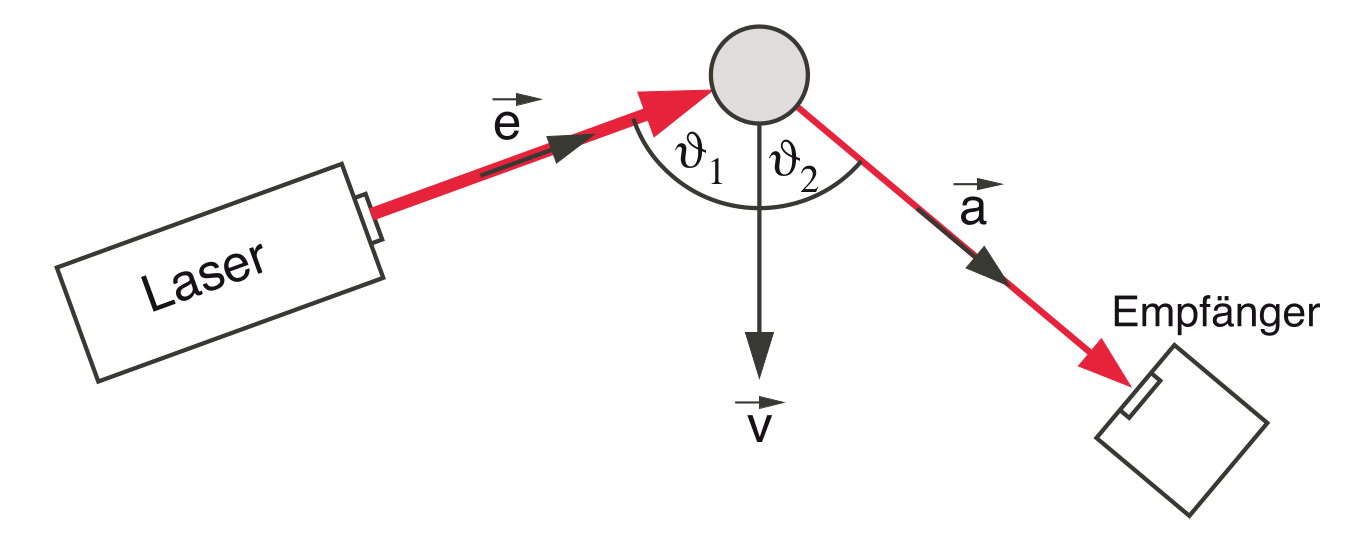
\includegraphics[width=0.67\textwidth]{images/doppler-effekt.png}
    \caption{%
        Dopplereffekt   mit  station\"arem   Sender,   bewegtem  Streuer   und
        station\"arem Detektor. \quelleVA
    }
    \label{fig:dopplereffekt}
\end{figure}

Da  bei  technischen  Geschwindigkeiten das  Verh\"altnis  $\frac{v}{c}$  sehr
klein   ist,  ergeben   sich  unter   solchen  Umst\"anden   lediglich  minime
Unterschide  in   den  Frequenzen  $f_4$,  $f_1$   und  $f_2$. Eine  pr\"azise
Messung  der  Frequenzunterschiede  ist  somit enorm  schwierig,  weshalb  man
sich  eines Zwei-Stral-Verfahrens  bedient. Da die  beiden Teilstrahlen  dabei
in  unterschiedlichen  Winkeln  $\vartheta_1$  (vgl. Formel  \ref{eq:doppler})
auf   das   streuende   Teilchen  treffen,   erfahren   sie   unterschiedliche
Doppler-Verschiebungen ihrer Frequenzen.

\"Uberlagert man  nun die beiden  Teilstrahlen in einem Detektor,  ergibt sich
eine  Schwebung, deren  Frequenz bedeutend  tiefer  als $f_0$  ist, und  somit
verh\"altnism\"assig gut detektiert werden kann.

Eine     h\"aufig     verwendete     Konfiguration    ist     in     Abbildung
\ref{fig:zweistrahl-anordnung} zu sehen.

\begin{figure}[h!t]
    \centering
    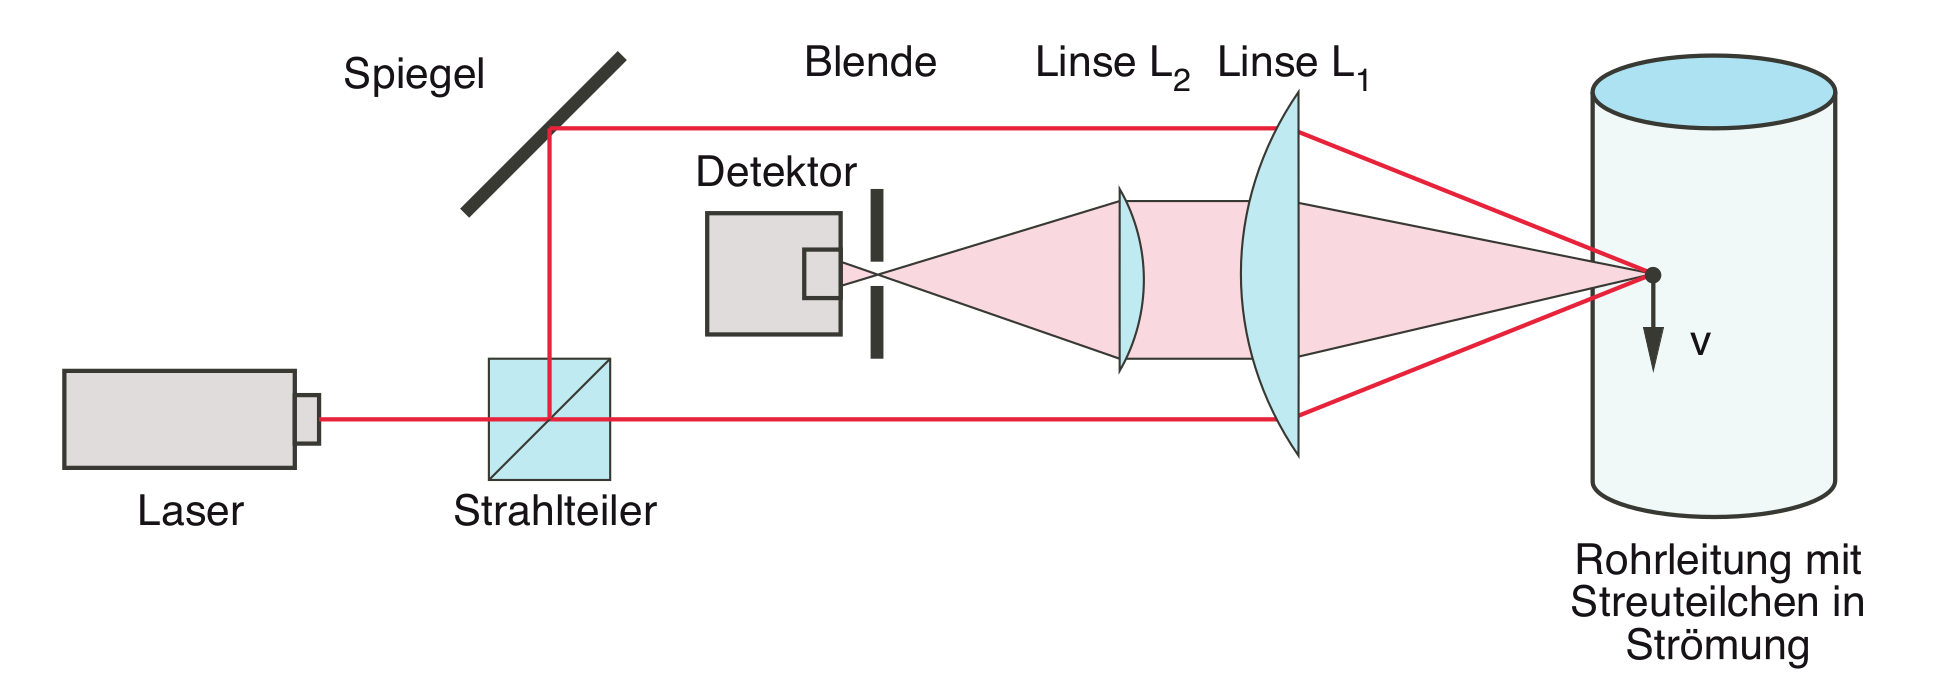
\includegraphics[width=0.67\textwidth]{images/zweistrahl-anordnung.png}
    \caption{%
        Zwei-Srahl-Anordnung. \quelleVA
    }
    \label{fig:zweistrahl-anordnung}
\end{figure}

Ein Strahlteiler teilt  den Laserstrahl auf zwei Strahlen auf  und ein Spiegel
sorgt daf\"ur, dass zwei parallele  Strahlen entstehen, die anschliessen durch
eine Linse $L_1$ mit Brennweite $f_1$ wieder zusammengef\"uhrt werden. Fliesst
ein Streuteilchen durch diesen Schnittpunkt, ergeben sich f\"ur die beiden Teilstrahlen
zwei unterschiedliche Frequenzen aufgrund des Dopplereffekts:

\begin{align}
    \label{eq:splitFreqs1}
        f_1 &= f_0 \cdot
            \left(
                1 + \frac{v}{c} \cdot \cos\left( \SI{90}{\degree} + \frac{\varphi}{2} \right)
            \right)
            =
            f_0 \cdot
            \left(
                1 - \frac{v}{c} \cdot \sin\left(\frac{\varphi}{2}\right)
            \right)
            \\
        \label{eq:splitFreqs2}
        f_2 &= f_0 \cdot
            \left(
                1 + \frac{v}{c} \cdot \cos\left( \SI{90}{\degree} - \frac{\varphi}{2} \right)
            \right)
            =
            f_0 \cdot
            \left(
                1 + \frac{v}{c} \cdot \sin\left(\frac{\varphi}{2}\right)
            \right)
            \\
        \label{eq:splitFreqsDelta}
        \Delta\,f &= f_2 - f_1 = f_0 \cdot \frac{2 \cdot v}{c} \cdot \sin\left( \frac{\varphi}{2}\right)
\end{align}

Die beiden  Wellenz\"uge werden  anschliessend in einem  einzelnen Empf\"anger
zusammengef\"uhrt. Die durch diese \"Uberlagerung erzeugte Schwebung errechnet
sich  nach  einigen  trigonometrischen  Umformungen zu  (beachte,  dass  beide
Signale die gleiche Amplitude haben, was die Sache etwas vereinfacht):

\begin{equation}
    \label{eq:schwebung}
    S(t) = A \cdot \cos(\omega_1 \cdot t) + A \cdot \cos(\omega_2 \cdot t)
         = 2 A \cdot
             \cos\left(
                 \frac{\omega_1 + \omega_2}{2} \cdot t
             \right)
             \cdot
             \cos\left(
                 \frac{\omega_1 - \omega_2}{2} \cdot t
             \right)
\end{equation}

Nun wird  in einem Detektor  jedoch nicht  die Schwebung selbst,  sondern ihre
Intensit\"at gemessen. Diese ist als das Quadrat der Schwebung definiert:

\begin{equation}
    \label{eq:intensity}
    \begin{split}
        I(t) &= S^2(t) \\
             &= A^2           \cdot \left( \cos^2(\omega_1 \cdot t) + \cos^2(\omega_2 \cdot t) + 2 \cdot \cos(\omega_1 \cdot t) \cdot \cos(\omega_2 \cdot t) \right) \\
             &= \frac{A^2}{2} \cdot \left( 1 + \cos(2\omega_1 \cdot t) + \cos(2\omega_2 \cdot t) + 4 \cdot \cos(\omega_1 \cdot t)\cos(\omega_2 \cdot t) \right) \\
             &= \frac{A^2}{2} \cdot \left( 2 + \cos(2\omega_1 \cdot t) + \cos(2\omega_2 \cdot t) + 2 \cdot \cos\left((\omega_1 + \omega_2) \cdot t \right) + 2 \cdot \cos\left( (\omega_1 - \omega_2) \cdot t \right) \right)
    \end{split}
\end{equation}

Der  Detektor ist  im Vergleich  zur Lichtfrequenz  ziemlich langsam  und kann
somit  die  Schwingungen  der h\"oheren  Frequenzen  $2\omega_1$,  $2\omega_2$
und  $\omega_1  +   \omega_2$  nicht  detektieren,  wohl   aber  die  langsame
Schwebungsfrequenz $\omega_1 - \omega_2$. Methematisch  kann man dies als eine
Mittelung \"uber  eine Zeit in  der Gr\"ossenordnung von  $\frac{1}{\abs{f_1 -
f_2}}$  betrachten.   In  diesem  Falle werden  die  schnelleren  Schwingungen
ausgemittelt  und verschwinden,  lediglich der  langsamste Anteil  bleibt noch
\"ubrig. Dies ergibt f\"ur das im Detektor ausgewertete Signal:

\begin{equation}
    \label{eq:schwebungResult}
    I^{*} = A^2 \cdot \bigg( 1 + \cos\Big((\omega_1 - \omega_2) \cdot t \Big) \bigg)
\end{equation}

\begin{figure}[h!t]
    \centering
    \resizebox{0.6\textwidth}{!}{%% Creator: Matplotlib, PGF backend
%%
%% To include the figure in your LaTeX document, write
%%   \input{<filename>.pgf}
%%
%% Make sure the required packages are loaded in your preamble
%%   \usepackage{pgf}
%%
%% Figures using additional raster images can only be included by \input if
%% they are in the same directory as the main LaTeX file. For loading figures
%% from other directories you can use the `import` package
%%   \usepackage{import}
%% and then include the figures with
%%   \import{<path to file>}{<filename>.pgf}
%%
%% Matplotlib used the following preamble
%%   \usepackage{fontspec}
%%   \setmainfont{Bitstream Vera Serif}
%%   \setsansfont{Bitstream Vera Sans}
%%   \setmonofont{Bitstream Vera Sans Mono}
%%
\begingroup%
\makeatletter%
\begin{pgfpicture}%
\pgfpathrectangle{\pgfpointorigin}{\pgfqpoint{10.000000in}{15.000000in}}%
\pgfusepath{use as bounding box, clip}%
\begin{pgfscope}%
\pgfsetbuttcap%
\pgfsetmiterjoin%
\definecolor{currentfill}{rgb}{1.000000,1.000000,1.000000}%
\pgfsetfillcolor{currentfill}%
\pgfsetlinewidth{0.000000pt}%
\definecolor{currentstroke}{rgb}{1.000000,1.000000,1.000000}%
\pgfsetstrokecolor{currentstroke}%
\pgfsetdash{}{0pt}%
\pgfpathmoveto{\pgfqpoint{0.000000in}{0.000000in}}%
\pgfpathlineto{\pgfqpoint{10.000000in}{0.000000in}}%
\pgfpathlineto{\pgfqpoint{10.000000in}{15.000000in}}%
\pgfpathlineto{\pgfqpoint{0.000000in}{15.000000in}}%
\pgfpathclose%
\pgfusepath{fill}%
\end{pgfscope}%
\begin{pgfscope}%
\pgfsetbuttcap%
\pgfsetmiterjoin%
\definecolor{currentfill}{rgb}{1.000000,1.000000,1.000000}%
\pgfsetfillcolor{currentfill}%
\pgfsetlinewidth{0.000000pt}%
\definecolor{currentstroke}{rgb}{0.000000,0.000000,0.000000}%
\pgfsetstrokecolor{currentstroke}%
\pgfsetstrokeopacity{0.000000}%
\pgfsetdash{}{0pt}%
\pgfpathmoveto{\pgfqpoint{0.500000in}{12.315517in}}%
\pgfpathlineto{\pgfqpoint{9.900000in}{12.315517in}}%
\pgfpathlineto{\pgfqpoint{9.900000in}{14.850000in}}%
\pgfpathlineto{\pgfqpoint{0.500000in}{14.850000in}}%
\pgfpathclose%
\pgfusepath{fill}%
\end{pgfscope}%
\begin{pgfscope}%
\pgfpathrectangle{\pgfqpoint{0.500000in}{12.315517in}}{\pgfqpoint{9.400000in}{2.534483in}} %
\pgfusepath{clip}%
\pgfsetrectcap%
\pgfsetroundjoin%
\pgfsetlinewidth{1.003750pt}%
\definecolor{currentstroke}{rgb}{0.000000,0.000000,1.000000}%
\pgfsetstrokecolor{currentstroke}%
\pgfsetdash{}{0pt}%
\pgfpathmoveto{\pgfqpoint{0.500000in}{14.850000in}}%
\pgfpathlineto{\pgfqpoint{0.509409in}{14.843593in}}%
\pgfpathlineto{\pgfqpoint{0.518819in}{14.824438in}}%
\pgfpathlineto{\pgfqpoint{0.528228in}{14.792729in}}%
\pgfpathlineto{\pgfqpoint{0.537638in}{14.748792in}}%
\pgfpathlineto{\pgfqpoint{0.547047in}{14.693074in}}%
\pgfpathlineto{\pgfqpoint{0.556456in}{14.626143in}}%
\pgfpathlineto{\pgfqpoint{0.565866in}{14.548683in}}%
\pgfpathlineto{\pgfqpoint{0.584685in}{14.365429in}}%
\pgfpathlineto{\pgfqpoint{0.603504in}{14.150757in}}%
\pgfpathlineto{\pgfqpoint{0.631732in}{13.789139in}}%
\pgfpathlineto{\pgfqpoint{0.688188in}{13.045728in}}%
\pgfpathlineto{\pgfqpoint{0.707007in}{12.828462in}}%
\pgfpathlineto{\pgfqpoint{0.725826in}{12.641500in}}%
\pgfpathlineto{\pgfqpoint{0.735235in}{12.561726in}}%
\pgfpathlineto{\pgfqpoint{0.744645in}{12.492152in}}%
\pgfpathlineto{\pgfqpoint{0.754054in}{12.433441in}}%
\pgfpathlineto{\pgfqpoint{0.763463in}{12.386145in}}%
\pgfpathlineto{\pgfqpoint{0.772873in}{12.350694in}}%
\pgfpathlineto{\pgfqpoint{0.782282in}{12.327396in}}%
\pgfpathlineto{\pgfqpoint{0.791692in}{12.316433in}}%
\pgfpathlineto{\pgfqpoint{0.801101in}{12.317860in}}%
\pgfpathlineto{\pgfqpoint{0.810511in}{12.331604in}}%
\pgfpathlineto{\pgfqpoint{0.819920in}{12.357463in}}%
\pgfpathlineto{\pgfqpoint{0.829329in}{12.395113in}}%
\pgfpathlineto{\pgfqpoint{0.838739in}{12.444111in}}%
\pgfpathlineto{\pgfqpoint{0.848148in}{12.503895in}}%
\pgfpathlineto{\pgfqpoint{0.857558in}{12.573796in}}%
\pgfpathlineto{\pgfqpoint{0.876376in}{12.740771in}}%
\pgfpathlineto{\pgfqpoint{0.895195in}{12.937800in}}%
\pgfpathlineto{\pgfqpoint{0.923423in}{13.271054in}}%
\pgfpathlineto{\pgfqpoint{0.970470in}{13.848168in}}%
\pgfpathlineto{\pgfqpoint{0.989289in}{14.058684in}}%
\pgfpathlineto{\pgfqpoint{1.008108in}{14.244303in}}%
\pgfpathlineto{\pgfqpoint{1.026927in}{14.397536in}}%
\pgfpathlineto{\pgfqpoint{1.036336in}{14.460042in}}%
\pgfpathlineto{\pgfqpoint{1.045746in}{14.512287in}}%
\pgfpathlineto{\pgfqpoint{1.055155in}{14.553768in}}%
\pgfpathlineto{\pgfqpoint{1.064565in}{14.584091in}}%
\pgfpathlineto{\pgfqpoint{1.073974in}{14.602981in}}%
\pgfpathlineto{\pgfqpoint{1.083383in}{14.610279in}}%
\pgfpathlineto{\pgfqpoint{1.092793in}{14.605947in}}%
\pgfpathlineto{\pgfqpoint{1.102202in}{14.590067in}}%
\pgfpathlineto{\pgfqpoint{1.111612in}{14.562835in}}%
\pgfpathlineto{\pgfqpoint{1.121021in}{14.524566in}}%
\pgfpathlineto{\pgfqpoint{1.130430in}{14.475683in}}%
\pgfpathlineto{\pgfqpoint{1.139840in}{14.416715in}}%
\pgfpathlineto{\pgfqpoint{1.149249in}{14.348292in}}%
\pgfpathlineto{\pgfqpoint{1.168068in}{14.186044in}}%
\pgfpathlineto{\pgfqpoint{1.186887in}{13.995664in}}%
\pgfpathlineto{\pgfqpoint{1.215115in}{13.674540in}}%
\pgfpathlineto{\pgfqpoint{1.271572in}{13.011439in}}%
\pgfpathlineto{\pgfqpoint{1.290390in}{12.815647in}}%
\pgfpathlineto{\pgfqpoint{1.309209in}{12.645180in}}%
\pgfpathlineto{\pgfqpoint{1.328028in}{12.506086in}}%
\pgfpathlineto{\pgfqpoint{1.337437in}{12.449816in}}%
\pgfpathlineto{\pgfqpoint{1.346847in}{12.403015in}}%
\pgfpathlineto{\pgfqpoint{1.356256in}{12.366018in}}%
\pgfpathlineto{\pgfqpoint{1.365666in}{12.339056in}}%
\pgfpathlineto{\pgfqpoint{1.375075in}{12.322256in}}%
\pgfpathlineto{\pgfqpoint{1.384484in}{12.315636in}}%
\pgfpathlineto{\pgfqpoint{1.393894in}{12.319111in}}%
\pgfpathlineto{\pgfqpoint{1.403303in}{12.332491in}}%
\pgfpathlineto{\pgfqpoint{1.412713in}{12.355486in}}%
\pgfpathlineto{\pgfqpoint{1.422122in}{12.387709in}}%
\pgfpathlineto{\pgfqpoint{1.431532in}{12.428683in}}%
\pgfpathlineto{\pgfqpoint{1.440941in}{12.477845in}}%
\pgfpathlineto{\pgfqpoint{1.450350in}{12.534552in}}%
\pgfpathlineto{\pgfqpoint{1.469169in}{12.667683in}}%
\pgfpathlineto{\pgfqpoint{1.487988in}{12.821666in}}%
\pgfpathlineto{\pgfqpoint{1.516216in}{13.076018in}}%
\pgfpathlineto{\pgfqpoint{1.553854in}{13.419062in}}%
\pgfpathlineto{\pgfqpoint{1.572673in}{13.575652in}}%
\pgfpathlineto{\pgfqpoint{1.591491in}{13.713415in}}%
\pgfpathlineto{\pgfqpoint{1.610310in}{13.826793in}}%
\pgfpathlineto{\pgfqpoint{1.619720in}{13.872906in}}%
\pgfpathlineto{\pgfqpoint{1.629129in}{13.911363in}}%
\pgfpathlineto{\pgfqpoint{1.638539in}{13.941814in}}%
\pgfpathlineto{\pgfqpoint{1.647948in}{13.963996in}}%
\pgfpathlineto{\pgfqpoint{1.657357in}{13.977734in}}%
\pgfpathlineto{\pgfqpoint{1.666767in}{13.982946in}}%
\pgfpathlineto{\pgfqpoint{1.676176in}{13.979636in}}%
\pgfpathlineto{\pgfqpoint{1.685586in}{13.967897in}}%
\pgfpathlineto{\pgfqpoint{1.694995in}{13.947908in}}%
\pgfpathlineto{\pgfqpoint{1.704404in}{13.919931in}}%
\pgfpathlineto{\pgfqpoint{1.713814in}{13.884306in}}%
\pgfpathlineto{\pgfqpoint{1.723223in}{13.841449in}}%
\pgfpathlineto{\pgfqpoint{1.732633in}{13.791844in}}%
\pgfpathlineto{\pgfqpoint{1.751451in}{13.674627in}}%
\pgfpathlineto{\pgfqpoint{1.770270in}{13.537660in}}%
\pgfpathlineto{\pgfqpoint{1.798498in}{13.307678in}}%
\pgfpathlineto{\pgfqpoint{1.854955in}{12.835072in}}%
\pgfpathlineto{\pgfqpoint{1.873774in}{12.695349in}}%
\pgfpathlineto{\pgfqpoint{1.892593in}{12.572964in}}%
\pgfpathlineto{\pgfqpoint{1.911411in}{12.471770in}}%
\pgfpathlineto{\pgfqpoint{1.920821in}{12.430049in}}%
\pgfpathlineto{\pgfqpoint{1.930230in}{12.394608in}}%
\pgfpathlineto{\pgfqpoint{1.939640in}{12.365629in}}%
\pgfpathlineto{\pgfqpoint{1.949049in}{12.343226in}}%
\pgfpathlineto{\pgfqpoint{1.958458in}{12.327440in}}%
\pgfpathlineto{\pgfqpoint{1.967868in}{12.318242in}}%
\pgfpathlineto{\pgfqpoint{1.977277in}{12.315536in}}%
\pgfpathlineto{\pgfqpoint{1.986687in}{12.319159in}}%
\pgfpathlineto{\pgfqpoint{1.996096in}{12.328884in}}%
\pgfpathlineto{\pgfqpoint{2.005506in}{12.344426in}}%
\pgfpathlineto{\pgfqpoint{2.014915in}{12.365442in}}%
\pgfpathlineto{\pgfqpoint{2.024324in}{12.391540in}}%
\pgfpathlineto{\pgfqpoint{2.033734in}{12.422284in}}%
\pgfpathlineto{\pgfqpoint{2.052553in}{12.495757in}}%
\pgfpathlineto{\pgfqpoint{2.071371in}{12.581668in}}%
\pgfpathlineto{\pgfqpoint{2.099600in}{12.723874in}}%
\pgfpathlineto{\pgfqpoint{2.137237in}{12.914028in}}%
\pgfpathlineto{\pgfqpoint{2.156056in}{12.999517in}}%
\pgfpathlineto{\pgfqpoint{2.174875in}{13.073582in}}%
\pgfpathlineto{\pgfqpoint{2.184284in}{13.105364in}}%
\pgfpathlineto{\pgfqpoint{2.193694in}{13.133222in}}%
\pgfpathlineto{\pgfqpoint{2.203103in}{13.156896in}}%
\pgfpathlineto{\pgfqpoint{2.212513in}{13.176180in}}%
\pgfpathlineto{\pgfqpoint{2.221922in}{13.190919in}}%
\pgfpathlineto{\pgfqpoint{2.231331in}{13.201011in}}%
\pgfpathlineto{\pgfqpoint{2.240741in}{13.206404in}}%
\pgfpathlineto{\pgfqpoint{2.250150in}{13.207100in}}%
\pgfpathlineto{\pgfqpoint{2.259560in}{13.203152in}}%
\pgfpathlineto{\pgfqpoint{2.268969in}{13.194658in}}%
\pgfpathlineto{\pgfqpoint{2.278378in}{13.181766in}}%
\pgfpathlineto{\pgfqpoint{2.287788in}{13.164667in}}%
\pgfpathlineto{\pgfqpoint{2.297197in}{13.143591in}}%
\pgfpathlineto{\pgfqpoint{2.306607in}{13.118805in}}%
\pgfpathlineto{\pgfqpoint{2.325425in}{13.059338in}}%
\pgfpathlineto{\pgfqpoint{2.344244in}{12.988994in}}%
\pgfpathlineto{\pgfqpoint{2.372472in}{12.869798in}}%
\pgfpathlineto{\pgfqpoint{2.428929in}{12.621807in}}%
\pgfpathlineto{\pgfqpoint{2.447748in}{12.547272in}}%
\pgfpathlineto{\pgfqpoint{2.466567in}{12.480940in}}%
\pgfpathlineto{\pgfqpoint{2.485385in}{12.424611in}}%
\pgfpathlineto{\pgfqpoint{2.504204in}{12.379546in}}%
\pgfpathlineto{\pgfqpoint{2.513614in}{12.361478in}}%
\pgfpathlineto{\pgfqpoint{2.523023in}{12.346444in}}%
\pgfpathlineto{\pgfqpoint{2.532432in}{12.334443in}}%
\pgfpathlineto{\pgfqpoint{2.541842in}{12.325443in}}%
\pgfpathlineto{\pgfqpoint{2.551251in}{12.319378in}}%
\pgfpathlineto{\pgfqpoint{2.560661in}{12.316151in}}%
\pgfpathlineto{\pgfqpoint{2.570070in}{12.315641in}}%
\pgfpathlineto{\pgfqpoint{2.579479in}{12.317697in}}%
\pgfpathlineto{\pgfqpoint{2.588889in}{12.322147in}}%
\pgfpathlineto{\pgfqpoint{2.598298in}{12.328799in}}%
\pgfpathlineto{\pgfqpoint{2.607708in}{12.337441in}}%
\pgfpathlineto{\pgfqpoint{2.626527in}{12.359790in}}%
\pgfpathlineto{\pgfqpoint{2.645345in}{12.387281in}}%
\pgfpathlineto{\pgfqpoint{2.673574in}{12.433803in}}%
\pgfpathlineto{\pgfqpoint{2.711211in}{12.495630in}}%
\pgfpathlineto{\pgfqpoint{2.730030in}{12.522646in}}%
\pgfpathlineto{\pgfqpoint{2.748849in}{12.545261in}}%
\pgfpathlineto{\pgfqpoint{2.767668in}{12.562514in}}%
\pgfpathlineto{\pgfqpoint{2.777077in}{12.568921in}}%
\pgfpathlineto{\pgfqpoint{2.786486in}{12.573780in}}%
\pgfpathlineto{\pgfqpoint{2.795896in}{12.577068in}}%
\pgfpathlineto{\pgfqpoint{2.805305in}{12.578780in}}%
\pgfpathlineto{\pgfqpoint{2.814715in}{12.578932in}}%
\pgfpathlineto{\pgfqpoint{2.824124in}{12.577559in}}%
\pgfpathlineto{\pgfqpoint{2.833534in}{12.574715in}}%
\pgfpathlineto{\pgfqpoint{2.842943in}{12.570466in}}%
\pgfpathlineto{\pgfqpoint{2.861762in}{12.558103in}}%
\pgfpathlineto{\pgfqpoint{2.880581in}{12.541279in}}%
\pgfpathlineto{\pgfqpoint{2.899399in}{12.520948in}}%
\pgfpathlineto{\pgfqpoint{2.927628in}{12.486163in}}%
\pgfpathlineto{\pgfqpoint{2.984084in}{12.413898in}}%
\pgfpathlineto{\pgfqpoint{3.012312in}{12.382326in}}%
\pgfpathlineto{\pgfqpoint{3.031131in}{12.364386in}}%
\pgfpathlineto{\pgfqpoint{3.049950in}{12.349315in}}%
\pgfpathlineto{\pgfqpoint{3.068769in}{12.337237in}}%
\pgfpathlineto{\pgfqpoint{3.087588in}{12.328106in}}%
\pgfpathlineto{\pgfqpoint{3.106406in}{12.321726in}}%
\pgfpathlineto{\pgfqpoint{3.125225in}{12.317784in}}%
\pgfpathlineto{\pgfqpoint{3.144044in}{12.315879in}}%
\pgfpathlineto{\pgfqpoint{3.172272in}{12.315850in}}%
\pgfpathlineto{\pgfqpoint{3.209910in}{12.318677in}}%
\pgfpathlineto{\pgfqpoint{3.266366in}{12.322946in}}%
\pgfpathlineto{\pgfqpoint{3.304004in}{12.323349in}}%
\pgfpathlineto{\pgfqpoint{3.351051in}{12.320987in}}%
\pgfpathlineto{\pgfqpoint{3.435736in}{12.315732in}}%
\pgfpathlineto{\pgfqpoint{3.473373in}{12.315809in}}%
\pgfpathlineto{\pgfqpoint{3.520420in}{12.318367in}}%
\pgfpathlineto{\pgfqpoint{3.595696in}{12.323185in}}%
\pgfpathlineto{\pgfqpoint{3.633333in}{12.323184in}}%
\pgfpathlineto{\pgfqpoint{3.670971in}{12.320949in}}%
\pgfpathlineto{\pgfqpoint{3.746246in}{12.315525in}}%
\pgfpathlineto{\pgfqpoint{3.765065in}{12.316059in}}%
\pgfpathlineto{\pgfqpoint{3.783884in}{12.318250in}}%
\pgfpathlineto{\pgfqpoint{3.802703in}{12.322545in}}%
\pgfpathlineto{\pgfqpoint{3.821522in}{12.329334in}}%
\pgfpathlineto{\pgfqpoint{3.840340in}{12.338912in}}%
\pgfpathlineto{\pgfqpoint{3.859159in}{12.351455in}}%
\pgfpathlineto{\pgfqpoint{3.877978in}{12.366983in}}%
\pgfpathlineto{\pgfqpoint{3.896797in}{12.385345in}}%
\pgfpathlineto{\pgfqpoint{3.915616in}{12.406207in}}%
\pgfpathlineto{\pgfqpoint{3.943844in}{12.441004in}}%
\pgfpathlineto{\pgfqpoint{4.000300in}{12.513306in}}%
\pgfpathlineto{\pgfqpoint{4.019119in}{12.534607in}}%
\pgfpathlineto{\pgfqpoint{4.037938in}{12.552755in}}%
\pgfpathlineto{\pgfqpoint{4.056757in}{12.566758in}}%
\pgfpathlineto{\pgfqpoint{4.066166in}{12.571928in}}%
\pgfpathlineto{\pgfqpoint{4.075576in}{12.575749in}}%
\pgfpathlineto{\pgfqpoint{4.084985in}{12.578145in}}%
\pgfpathlineto{\pgfqpoint{4.094394in}{12.579050in}}%
\pgfpathlineto{\pgfqpoint{4.103804in}{12.578417in}}%
\pgfpathlineto{\pgfqpoint{4.113213in}{12.576218in}}%
\pgfpathlineto{\pgfqpoint{4.122623in}{12.572442in}}%
\pgfpathlineto{\pgfqpoint{4.132032in}{12.567100in}}%
\pgfpathlineto{\pgfqpoint{4.141441in}{12.560222in}}%
\pgfpathlineto{\pgfqpoint{4.160260in}{12.542089in}}%
\pgfpathlineto{\pgfqpoint{4.179079in}{12.518720in}}%
\pgfpathlineto{\pgfqpoint{4.197898in}{12.491131in}}%
\pgfpathlineto{\pgfqpoint{4.226126in}{12.444810in}}%
\pgfpathlineto{\pgfqpoint{4.263764in}{12.382766in}}%
\pgfpathlineto{\pgfqpoint{4.282583in}{12.355942in}}%
\pgfpathlineto{\pgfqpoint{4.301401in}{12.334564in}}%
\pgfpathlineto{\pgfqpoint{4.310811in}{12.326515in}}%
\pgfpathlineto{\pgfqpoint{4.320220in}{12.320524in}}%
\pgfpathlineto{\pgfqpoint{4.329630in}{12.316796in}}%
\pgfpathlineto{\pgfqpoint{4.339039in}{12.315517in}}%
\pgfpathlineto{\pgfqpoint{4.348448in}{12.316854in}}%
\pgfpathlineto{\pgfqpoint{4.357858in}{12.320948in}}%
\pgfpathlineto{\pgfqpoint{4.367267in}{12.327914in}}%
\pgfpathlineto{\pgfqpoint{4.376677in}{12.337838in}}%
\pgfpathlineto{\pgfqpoint{4.386086in}{12.350776in}}%
\pgfpathlineto{\pgfqpoint{4.395495in}{12.366752in}}%
\pgfpathlineto{\pgfqpoint{4.404905in}{12.385755in}}%
\pgfpathlineto{\pgfqpoint{4.414314in}{12.407739in}}%
\pgfpathlineto{\pgfqpoint{4.433133in}{12.460295in}}%
\pgfpathlineto{\pgfqpoint{4.451952in}{12.523352in}}%
\pgfpathlineto{\pgfqpoint{4.470771in}{12.595291in}}%
\pgfpathlineto{\pgfqpoint{4.498999in}{12.715079in}}%
\pgfpathlineto{\pgfqpoint{4.555455in}{12.962739in}}%
\pgfpathlineto{\pgfqpoint{4.574274in}{13.036142in}}%
\pgfpathlineto{\pgfqpoint{4.593093in}{13.099690in}}%
\pgfpathlineto{\pgfqpoint{4.602503in}{13.126862in}}%
\pgfpathlineto{\pgfqpoint{4.611912in}{13.150530in}}%
\pgfpathlineto{\pgfqpoint{4.621321in}{13.170401in}}%
\pgfpathlineto{\pgfqpoint{4.630731in}{13.186220in}}%
\pgfpathlineto{\pgfqpoint{4.640140in}{13.197767in}}%
\pgfpathlineto{\pgfqpoint{4.649550in}{13.204867in}}%
\pgfpathlineto{\pgfqpoint{4.658959in}{13.207385in}}%
\pgfpathlineto{\pgfqpoint{4.668368in}{13.205237in}}%
\pgfpathlineto{\pgfqpoint{4.677778in}{13.198386in}}%
\pgfpathlineto{\pgfqpoint{4.687187in}{13.186847in}}%
\pgfpathlineto{\pgfqpoint{4.696597in}{13.170686in}}%
\pgfpathlineto{\pgfqpoint{4.706006in}{13.150023in}}%
\pgfpathlineto{\pgfqpoint{4.715415in}{13.125028in}}%
\pgfpathlineto{\pgfqpoint{4.724825in}{13.095925in}}%
\pgfpathlineto{\pgfqpoint{4.743644in}{13.026535in}}%
\pgfpathlineto{\pgfqpoint{4.762462in}{12.944606in}}%
\pgfpathlineto{\pgfqpoint{4.790691in}{12.805880in}}%
\pgfpathlineto{\pgfqpoint{4.837738in}{12.567727in}}%
\pgfpathlineto{\pgfqpoint{4.856557in}{12.483452in}}%
\pgfpathlineto{\pgfqpoint{4.875375in}{12.412291in}}%
\pgfpathlineto{\pgfqpoint{4.884785in}{12.382938in}}%
\pgfpathlineto{\pgfqpoint{4.894194in}{12.358369in}}%
\pgfpathlineto{\pgfqpoint{4.903604in}{12.339009in}}%
\pgfpathlineto{\pgfqpoint{4.913013in}{12.325235in}}%
\pgfpathlineto{\pgfqpoint{4.922422in}{12.317373in}}%
\pgfpathlineto{\pgfqpoint{4.931832in}{12.315689in}}%
\pgfpathlineto{\pgfqpoint{4.941241in}{12.320391in}}%
\pgfpathlineto{\pgfqpoint{4.950651in}{12.331623in}}%
\pgfpathlineto{\pgfqpoint{4.960060in}{12.349459in}}%
\pgfpathlineto{\pgfqpoint{4.969469in}{12.373907in}}%
\pgfpathlineto{\pgfqpoint{4.978879in}{12.404903in}}%
\pgfpathlineto{\pgfqpoint{4.988288in}{12.442313in}}%
\pgfpathlineto{\pgfqpoint{4.997698in}{12.485931in}}%
\pgfpathlineto{\pgfqpoint{5.016517in}{12.590620in}}%
\pgfpathlineto{\pgfqpoint{5.035335in}{12.715966in}}%
\pgfpathlineto{\pgfqpoint{5.054154in}{12.857972in}}%
\pgfpathlineto{\pgfqpoint{5.082382in}{13.091417in}}%
\pgfpathlineto{\pgfqpoint{5.129429in}{13.486820in}}%
\pgfpathlineto{\pgfqpoint{5.148248in}{13.629315in}}%
\pgfpathlineto{\pgfqpoint{5.167067in}{13.753952in}}%
\pgfpathlineto{\pgfqpoint{5.185886in}{13.855471in}}%
\pgfpathlineto{\pgfqpoint{5.195295in}{13.896137in}}%
\pgfpathlineto{\pgfqpoint{5.204705in}{13.929433in}}%
\pgfpathlineto{\pgfqpoint{5.214114in}{13.954968in}}%
\pgfpathlineto{\pgfqpoint{5.223524in}{13.972425in}}%
\pgfpathlineto{\pgfqpoint{5.232933in}{13.981568in}}%
\pgfpathlineto{\pgfqpoint{5.242342in}{13.982244in}}%
\pgfpathlineto{\pgfqpoint{5.251752in}{13.974388in}}%
\pgfpathlineto{\pgfqpoint{5.261161in}{13.958020in}}%
\pgfpathlineto{\pgfqpoint{5.270571in}{13.933254in}}%
\pgfpathlineto{\pgfqpoint{5.279980in}{13.900291in}}%
\pgfpathlineto{\pgfqpoint{5.289389in}{13.859421in}}%
\pgfpathlineto{\pgfqpoint{5.298799in}{13.811020in}}%
\pgfpathlineto{\pgfqpoint{5.317618in}{13.693544in}}%
\pgfpathlineto{\pgfqpoint{5.336436in}{13.552476in}}%
\pgfpathlineto{\pgfqpoint{5.355255in}{13.393530in}}%
\pgfpathlineto{\pgfqpoint{5.392893in}{13.049068in}}%
\pgfpathlineto{\pgfqpoint{5.421121in}{12.796731in}}%
\pgfpathlineto{\pgfqpoint{5.439940in}{12.645526in}}%
\pgfpathlineto{\pgfqpoint{5.458759in}{12.516220in}}%
\pgfpathlineto{\pgfqpoint{5.468168in}{12.461777in}}%
\pgfpathlineto{\pgfqpoint{5.477578in}{12.415087in}}%
\pgfpathlineto{\pgfqpoint{5.486987in}{12.376767in}}%
\pgfpathlineto{\pgfqpoint{5.496396in}{12.347356in}}%
\pgfpathlineto{\pgfqpoint{5.505806in}{12.327302in}}%
\pgfpathlineto{\pgfqpoint{5.515215in}{12.316965in}}%
\pgfpathlineto{\pgfqpoint{5.524625in}{12.316602in}}%
\pgfpathlineto{\pgfqpoint{5.534034in}{12.326371in}}%
\pgfpathlineto{\pgfqpoint{5.543443in}{12.346326in}}%
\pgfpathlineto{\pgfqpoint{5.552853in}{12.376415in}}%
\pgfpathlineto{\pgfqpoint{5.562262in}{12.416479in}}%
\pgfpathlineto{\pgfqpoint{5.571672in}{12.466254in}}%
\pgfpathlineto{\pgfqpoint{5.581081in}{12.525372in}}%
\pgfpathlineto{\pgfqpoint{5.590490in}{12.593366in}}%
\pgfpathlineto{\pgfqpoint{5.609309in}{12.753623in}}%
\pgfpathlineto{\pgfqpoint{5.628128in}{12.941436in}}%
\pgfpathlineto{\pgfqpoint{5.656356in}{13.259584in}}%
\pgfpathlineto{\pgfqpoint{5.712813in}{13.924818in}}%
\pgfpathlineto{\pgfqpoint{5.731632in}{14.123147in}}%
\pgfpathlineto{\pgfqpoint{5.750450in}{14.295923in}}%
\pgfpathlineto{\pgfqpoint{5.759860in}{14.370458in}}%
\pgfpathlineto{\pgfqpoint{5.769269in}{14.436025in}}%
\pgfpathlineto{\pgfqpoint{5.778679in}{14.491931in}}%
\pgfpathlineto{\pgfqpoint{5.788088in}{14.537578in}}%
\pgfpathlineto{\pgfqpoint{5.797497in}{14.572468in}}%
\pgfpathlineto{\pgfqpoint{5.806907in}{14.596211in}}%
\pgfpathlineto{\pgfqpoint{5.816316in}{14.608530in}}%
\pgfpathlineto{\pgfqpoint{5.825726in}{14.609262in}}%
\pgfpathlineto{\pgfqpoint{5.835135in}{14.598363in}}%
\pgfpathlineto{\pgfqpoint{5.844545in}{14.575909in}}%
\pgfpathlineto{\pgfqpoint{5.853954in}{14.542095in}}%
\pgfpathlineto{\pgfqpoint{5.863363in}{14.497232in}}%
\pgfpathlineto{\pgfqpoint{5.872773in}{14.441748in}}%
\pgfpathlineto{\pgfqpoint{5.882182in}{14.376184in}}%
\pgfpathlineto{\pgfqpoint{5.901001in}{14.217498in}}%
\pgfpathlineto{\pgfqpoint{5.919820in}{14.027500in}}%
\pgfpathlineto{\pgfqpoint{5.938639in}{13.813873in}}%
\pgfpathlineto{\pgfqpoint{5.976276in}{13.351324in}}%
\pgfpathlineto{\pgfqpoint{6.004505in}{13.011274in}}%
\pgfpathlineto{\pgfqpoint{6.023323in}{12.805776in}}%
\pgfpathlineto{\pgfqpoint{6.042142in}{12.627544in}}%
\pgfpathlineto{\pgfqpoint{6.051552in}{12.551104in}}%
\pgfpathlineto{\pgfqpoint{6.060961in}{12.484259in}}%
\pgfpathlineto{\pgfqpoint{6.070370in}{12.427750in}}%
\pgfpathlineto{\pgfqpoint{6.079780in}{12.382213in}}%
\pgfpathlineto{\pgfqpoint{6.089189in}{12.348174in}}%
\pgfpathlineto{\pgfqpoint{6.098599in}{12.326039in}}%
\pgfpathlineto{\pgfqpoint{6.108008in}{12.316096in}}%
\pgfpathlineto{\pgfqpoint{6.117417in}{12.318505in}}%
\pgfpathlineto{\pgfqpoint{6.126827in}{12.333301in}}%
\pgfpathlineto{\pgfqpoint{6.136236in}{12.360389in}}%
\pgfpathlineto{\pgfqpoint{6.145646in}{12.399548in}}%
\pgfpathlineto{\pgfqpoint{6.155055in}{12.450432in}}%
\pgfpathlineto{\pgfqpoint{6.164464in}{12.512573in}}%
\pgfpathlineto{\pgfqpoint{6.173874in}{12.585383in}}%
\pgfpathlineto{\pgfqpoint{6.192693in}{12.760115in}}%
\pgfpathlineto{\pgfqpoint{6.211512in}{12.967836in}}%
\pgfpathlineto{\pgfqpoint{6.230330in}{13.200359in}}%
\pgfpathlineto{\pgfqpoint{6.277377in}{13.827900in}}%
\pgfpathlineto{\pgfqpoint{6.305606in}{14.185726in}}%
\pgfpathlineto{\pgfqpoint{6.324424in}{14.396074in}}%
\pgfpathlineto{\pgfqpoint{6.343243in}{14.573759in}}%
\pgfpathlineto{\pgfqpoint{6.352653in}{14.648037in}}%
\pgfpathlineto{\pgfqpoint{6.362062in}{14.711562in}}%
\pgfpathlineto{\pgfqpoint{6.371471in}{14.763686in}}%
\pgfpathlineto{\pgfqpoint{6.380881in}{14.803877in}}%
\pgfpathlineto{\pgfqpoint{6.390290in}{14.831726in}}%
\pgfpathlineto{\pgfqpoint{6.399700in}{14.846946in}}%
\pgfpathlineto{\pgfqpoint{6.409109in}{14.849385in}}%
\pgfpathlineto{\pgfqpoint{6.418519in}{14.839015in}}%
\pgfpathlineto{\pgfqpoint{6.427928in}{14.815944in}}%
\pgfpathlineto{\pgfqpoint{6.437337in}{14.780407in}}%
\pgfpathlineto{\pgfqpoint{6.446747in}{14.732766in}}%
\pgfpathlineto{\pgfqpoint{6.456156in}{14.673509in}}%
\pgfpathlineto{\pgfqpoint{6.465566in}{14.603238in}}%
\pgfpathlineto{\pgfqpoint{6.484384in}{14.432628in}}%
\pgfpathlineto{\pgfqpoint{6.503203in}{14.227872in}}%
\pgfpathlineto{\pgfqpoint{6.522022in}{13.997277in}}%
\pgfpathlineto{\pgfqpoint{6.559660in}{13.496569in}}%
\pgfpathlineto{\pgfqpoint{6.587888in}{13.126215in}}%
\pgfpathlineto{\pgfqpoint{6.606707in}{12.900429in}}%
\pgfpathlineto{\pgfqpoint{6.625526in}{12.702111in}}%
\pgfpathlineto{\pgfqpoint{6.644344in}{12.539049in}}%
\pgfpathlineto{\pgfqpoint{6.653754in}{12.472775in}}%
\pgfpathlineto{\pgfqpoint{6.663163in}{12.417547in}}%
\pgfpathlineto{\pgfqpoint{6.672573in}{12.373879in}}%
\pgfpathlineto{\pgfqpoint{6.681982in}{12.342166in}}%
\pgfpathlineto{\pgfqpoint{6.691391in}{12.322676in}}%
\pgfpathlineto{\pgfqpoint{6.700801in}{12.315552in}}%
\pgfpathlineto{\pgfqpoint{6.710210in}{12.320808in}}%
\pgfpathlineto{\pgfqpoint{6.719620in}{12.338332in}}%
\pgfpathlineto{\pgfqpoint{6.729029in}{12.367884in}}%
\pgfpathlineto{\pgfqpoint{6.738438in}{12.409103in}}%
\pgfpathlineto{\pgfqpoint{6.747848in}{12.461507in}}%
\pgfpathlineto{\pgfqpoint{6.757257in}{12.524502in}}%
\pgfpathlineto{\pgfqpoint{6.766667in}{12.597385in}}%
\pgfpathlineto{\pgfqpoint{6.785485in}{12.769522in}}%
\pgfpathlineto{\pgfqpoint{6.804304in}{12.970480in}}%
\pgfpathlineto{\pgfqpoint{6.832533in}{13.306993in}}%
\pgfpathlineto{\pgfqpoint{6.879580in}{13.882070in}}%
\pgfpathlineto{\pgfqpoint{6.898398in}{14.089268in}}%
\pgfpathlineto{\pgfqpoint{6.917217in}{14.270329in}}%
\pgfpathlineto{\pgfqpoint{6.936036in}{14.417962in}}%
\pgfpathlineto{\pgfqpoint{6.945445in}{14.477349in}}%
\pgfpathlineto{\pgfqpoint{6.954855in}{14.526309in}}%
\pgfpathlineto{\pgfqpoint{6.964264in}{14.564370in}}%
\pgfpathlineto{\pgfqpoint{6.973674in}{14.591175in}}%
\pgfpathlineto{\pgfqpoint{6.983083in}{14.606485in}}%
\pgfpathlineto{\pgfqpoint{6.992492in}{14.610179in}}%
\pgfpathlineto{\pgfqpoint{7.001902in}{14.602255in}}%
\pgfpathlineto{\pgfqpoint{7.011311in}{14.582832in}}%
\pgfpathlineto{\pgfqpoint{7.020721in}{14.552143in}}%
\pgfpathlineto{\pgfqpoint{7.030130in}{14.510535in}}%
\pgfpathlineto{\pgfqpoint{7.039540in}{14.458466in}}%
\pgfpathlineto{\pgfqpoint{7.048949in}{14.396498in}}%
\pgfpathlineto{\pgfqpoint{7.058358in}{14.325287in}}%
\pgfpathlineto{\pgfqpoint{7.077177in}{14.158212in}}%
\pgfpathlineto{\pgfqpoint{7.095996in}{13.964147in}}%
\pgfpathlineto{\pgfqpoint{7.124224in}{13.639913in}}%
\pgfpathlineto{\pgfqpoint{7.171271in}{13.083606in}}%
\pgfpathlineto{\pgfqpoint{7.190090in}{12.880698in}}%
\pgfpathlineto{\pgfqpoint{7.208909in}{12.700743in}}%
\pgfpathlineto{\pgfqpoint{7.227728in}{12.550221in}}%
\pgfpathlineto{\pgfqpoint{7.237137in}{12.487666in}}%
\pgfpathlineto{\pgfqpoint{7.246547in}{12.434288in}}%
\pgfpathlineto{\pgfqpoint{7.255956in}{12.390492in}}%
\pgfpathlineto{\pgfqpoint{7.265365in}{12.356584in}}%
\pgfpathlineto{\pgfqpoint{7.274775in}{12.332762in}}%
\pgfpathlineto{\pgfqpoint{7.284184in}{12.319119in}}%
\pgfpathlineto{\pgfqpoint{7.293594in}{12.315640in}}%
\pgfpathlineto{\pgfqpoint{7.303003in}{12.322208in}}%
\pgfpathlineto{\pgfqpoint{7.312412in}{12.338602in}}%
\pgfpathlineto{\pgfqpoint{7.321822in}{12.364502in}}%
\pgfpathlineto{\pgfqpoint{7.331231in}{12.399492in}}%
\pgfpathlineto{\pgfqpoint{7.340641in}{12.443066in}}%
\pgfpathlineto{\pgfqpoint{7.350050in}{12.494637in}}%
\pgfpathlineto{\pgfqpoint{7.368869in}{12.619040in}}%
\pgfpathlineto{\pgfqpoint{7.387688in}{12.766602in}}%
\pgfpathlineto{\pgfqpoint{7.415916in}{13.016091in}}%
\pgfpathlineto{\pgfqpoint{7.462963in}{13.444298in}}%
\pgfpathlineto{\pgfqpoint{7.481782in}{13.598375in}}%
\pgfpathlineto{\pgfqpoint{7.500601in}{13.732698in}}%
\pgfpathlineto{\pgfqpoint{7.519419in}{13.841872in}}%
\pgfpathlineto{\pgfqpoint{7.528829in}{13.885657in}}%
\pgfpathlineto{\pgfqpoint{7.538238in}{13.921667in}}%
\pgfpathlineto{\pgfqpoint{7.547648in}{13.949580in}}%
\pgfpathlineto{\pgfqpoint{7.557057in}{13.969160in}}%
\pgfpathlineto{\pgfqpoint{7.566466in}{13.980262in}}%
\pgfpathlineto{\pgfqpoint{7.575876in}{13.982829in}}%
\pgfpathlineto{\pgfqpoint{7.585285in}{13.976894in}}%
\pgfpathlineto{\pgfqpoint{7.594695in}{13.962576in}}%
\pgfpathlineto{\pgfqpoint{7.604104in}{13.940081in}}%
\pgfpathlineto{\pgfqpoint{7.613514in}{13.909695in}}%
\pgfpathlineto{\pgfqpoint{7.622923in}{13.871782in}}%
\pgfpathlineto{\pgfqpoint{7.632332in}{13.826779in}}%
\pgfpathlineto{\pgfqpoint{7.651151in}{13.717581in}}%
\pgfpathlineto{\pgfqpoint{7.669970in}{13.586818in}}%
\pgfpathlineto{\pgfqpoint{7.688789in}{13.439953in}}%
\pgfpathlineto{\pgfqpoint{7.726426in}{13.121972in}}%
\pgfpathlineto{\pgfqpoint{7.754655in}{12.886481in}}%
\pgfpathlineto{\pgfqpoint{7.773473in}{12.741832in}}%
\pgfpathlineto{\pgfqpoint{7.792292in}{12.612981in}}%
\pgfpathlineto{\pgfqpoint{7.811111in}{12.504099in}}%
\pgfpathlineto{\pgfqpoint{7.820521in}{12.458188in}}%
\pgfpathlineto{\pgfqpoint{7.829930in}{12.418389in}}%
\pgfpathlineto{\pgfqpoint{7.839339in}{12.384933in}}%
\pgfpathlineto{\pgfqpoint{7.848749in}{12.357983in}}%
\pgfpathlineto{\pgfqpoint{7.858158in}{12.337628in}}%
\pgfpathlineto{\pgfqpoint{7.867568in}{12.323889in}}%
\pgfpathlineto{\pgfqpoint{7.876977in}{12.316716in}}%
\pgfpathlineto{\pgfqpoint{7.886386in}{12.315991in}}%
\pgfpathlineto{\pgfqpoint{7.895796in}{12.321532in}}%
\pgfpathlineto{\pgfqpoint{7.905205in}{12.333092in}}%
\pgfpathlineto{\pgfqpoint{7.914615in}{12.350368in}}%
\pgfpathlineto{\pgfqpoint{7.924024in}{12.373003in}}%
\pgfpathlineto{\pgfqpoint{7.933433in}{12.400589in}}%
\pgfpathlineto{\pgfqpoint{7.942843in}{12.432676in}}%
\pgfpathlineto{\pgfqpoint{7.961662in}{12.508362in}}%
\pgfpathlineto{\pgfqpoint{7.980480in}{12.595798in}}%
\pgfpathlineto{\pgfqpoint{8.018118in}{12.787510in}}%
\pgfpathlineto{\pgfqpoint{8.046346in}{12.927877in}}%
\pgfpathlineto{\pgfqpoint{8.065165in}{13.011821in}}%
\pgfpathlineto{\pgfqpoint{8.083984in}{13.083830in}}%
\pgfpathlineto{\pgfqpoint{8.093393in}{13.114427in}}%
\pgfpathlineto{\pgfqpoint{8.102803in}{13.141013in}}%
\pgfpathlineto{\pgfqpoint{8.112212in}{13.163348in}}%
\pgfpathlineto{\pgfqpoint{8.121622in}{13.181238in}}%
\pgfpathlineto{\pgfqpoint{8.131031in}{13.194546in}}%
\pgfpathlineto{\pgfqpoint{8.140440in}{13.203185in}}%
\pgfpathlineto{\pgfqpoint{8.149850in}{13.207121in}}%
\pgfpathlineto{\pgfqpoint{8.159259in}{13.206370in}}%
\pgfpathlineto{\pgfqpoint{8.168669in}{13.201000in}}%
\pgfpathlineto{\pgfqpoint{8.178078in}{13.191127in}}%
\pgfpathlineto{\pgfqpoint{8.187487in}{13.176909in}}%
\pgfpathlineto{\pgfqpoint{8.196897in}{13.158551in}}%
\pgfpathlineto{\pgfqpoint{8.206306in}{13.136295in}}%
\pgfpathlineto{\pgfqpoint{8.215716in}{13.110420in}}%
\pgfpathlineto{\pgfqpoint{8.234535in}{13.049080in}}%
\pgfpathlineto{\pgfqpoint{8.253353in}{12.977318in}}%
\pgfpathlineto{\pgfqpoint{8.281582in}{12.856920in}}%
\pgfpathlineto{\pgfqpoint{8.338038in}{12.609812in}}%
\pgfpathlineto{\pgfqpoint{8.356857in}{12.536410in}}%
\pgfpathlineto{\pgfqpoint{8.375676in}{12.471522in}}%
\pgfpathlineto{\pgfqpoint{8.394494in}{12.416869in}}%
\pgfpathlineto{\pgfqpoint{8.403904in}{12.393770in}}%
\pgfpathlineto{\pgfqpoint{8.413313in}{12.373626in}}%
\pgfpathlineto{\pgfqpoint{8.422723in}{12.356496in}}%
\pgfpathlineto{\pgfqpoint{8.432132in}{12.342403in}}%
\pgfpathlineto{\pgfqpoint{8.441542in}{12.331337in}}%
\pgfpathlineto{\pgfqpoint{8.450951in}{12.323254in}}%
\pgfpathlineto{\pgfqpoint{8.460360in}{12.318080in}}%
\pgfpathlineto{\pgfqpoint{8.469770in}{12.315709in}}%
\pgfpathlineto{\pgfqpoint{8.479179in}{12.316011in}}%
\pgfpathlineto{\pgfqpoint{8.488589in}{12.318828in}}%
\pgfpathlineto{\pgfqpoint{8.497998in}{12.323982in}}%
\pgfpathlineto{\pgfqpoint{8.507407in}{12.331273in}}%
\pgfpathlineto{\pgfqpoint{8.516817in}{12.340488in}}%
\pgfpathlineto{\pgfqpoint{8.535636in}{12.363762in}}%
\pgfpathlineto{\pgfqpoint{8.554454in}{12.391872in}}%
\pgfpathlineto{\pgfqpoint{8.592092in}{12.454649in}}%
\pgfpathlineto{\pgfqpoint{8.620320in}{12.500055in}}%
\pgfpathlineto{\pgfqpoint{8.639139in}{12.526465in}}%
\pgfpathlineto{\pgfqpoint{8.657958in}{12.548304in}}%
\pgfpathlineto{\pgfqpoint{8.676777in}{12.564662in}}%
\pgfpathlineto{\pgfqpoint{8.686186in}{12.570593in}}%
\pgfpathlineto{\pgfqpoint{8.695596in}{12.574968in}}%
\pgfpathlineto{\pgfqpoint{8.705005in}{12.577766in}}%
\pgfpathlineto{\pgfqpoint{8.714414in}{12.578992in}}%
\pgfpathlineto{\pgfqpoint{8.723824in}{12.578668in}}%
\pgfpathlineto{\pgfqpoint{8.733233in}{12.576833in}}%
\pgfpathlineto{\pgfqpoint{8.742643in}{12.573545in}}%
\pgfpathlineto{\pgfqpoint{8.752052in}{12.568878in}}%
\pgfpathlineto{\pgfqpoint{8.770871in}{12.555766in}}%
\pgfpathlineto{\pgfqpoint{8.789690in}{12.538333in}}%
\pgfpathlineto{\pgfqpoint{8.808509in}{12.517552in}}%
\pgfpathlineto{\pgfqpoint{8.836737in}{12.482399in}}%
\pgfpathlineto{\pgfqpoint{8.893193in}{12.410418in}}%
\pgfpathlineto{\pgfqpoint{8.921421in}{12.379370in}}%
\pgfpathlineto{\pgfqpoint{8.940240in}{12.361859in}}%
\pgfpathlineto{\pgfqpoint{8.959059in}{12.347248in}}%
\pgfpathlineto{\pgfqpoint{8.977878in}{12.335633in}}%
\pgfpathlineto{\pgfqpoint{8.996697in}{12.326944in}}%
\pgfpathlineto{\pgfqpoint{9.015516in}{12.320965in}}%
\pgfpathlineto{\pgfqpoint{9.034334in}{12.317366in}}%
\pgfpathlineto{\pgfqpoint{9.053153in}{12.315738in}}%
\pgfpathlineto{\pgfqpoint{9.081381in}{12.315987in}}%
\pgfpathlineto{\pgfqpoint{9.128428in}{12.319814in}}%
\pgfpathlineto{\pgfqpoint{9.175475in}{12.323061in}}%
\pgfpathlineto{\pgfqpoint{9.213113in}{12.323283in}}%
\pgfpathlineto{\pgfqpoint{9.260160in}{12.320775in}}%
\pgfpathlineto{\pgfqpoint{9.335435in}{12.315919in}}%
\pgfpathlineto{\pgfqpoint{9.373073in}{12.315653in}}%
\pgfpathlineto{\pgfqpoint{9.420120in}{12.317902in}}%
\pgfpathlineto{\pgfqpoint{9.504805in}{12.323267in}}%
\pgfpathlineto{\pgfqpoint{9.542442in}{12.323086in}}%
\pgfpathlineto{\pgfqpoint{9.580080in}{12.320704in}}%
\pgfpathlineto{\pgfqpoint{9.645946in}{12.315641in}}%
\pgfpathlineto{\pgfqpoint{9.674174in}{12.316278in}}%
\pgfpathlineto{\pgfqpoint{9.692993in}{12.318767in}}%
\pgfpathlineto{\pgfqpoint{9.711812in}{12.323425in}}%
\pgfpathlineto{\pgfqpoint{9.730631in}{12.330629in}}%
\pgfpathlineto{\pgfqpoint{9.749449in}{12.340659in}}%
\pgfpathlineto{\pgfqpoint{9.768268in}{12.353666in}}%
\pgfpathlineto{\pgfqpoint{9.787087in}{12.369648in}}%
\pgfpathlineto{\pgfqpoint{9.805906in}{12.388424in}}%
\pgfpathlineto{\pgfqpoint{9.834134in}{12.420983in}}%
\pgfpathlineto{\pgfqpoint{9.871772in}{12.469281in}}%
\pgfpathlineto{\pgfqpoint{9.900000in}{12.505413in}}%
\pgfpathlineto{\pgfqpoint{9.900000in}{12.505413in}}%
\pgfusepath{stroke}%
\end{pgfscope}%
\begin{pgfscope}%
\pgfsetrectcap%
\pgfsetmiterjoin%
\pgfsetlinewidth{1.003750pt}%
\definecolor{currentstroke}{rgb}{0.000000,0.000000,0.000000}%
\pgfsetstrokecolor{currentstroke}%
\pgfsetdash{}{0pt}%
\pgfpathmoveto{\pgfqpoint{9.900000in}{12.315517in}}%
\pgfpathlineto{\pgfqpoint{9.900000in}{14.850000in}}%
\pgfusepath{stroke}%
\end{pgfscope}%
\begin{pgfscope}%
\pgfsetrectcap%
\pgfsetmiterjoin%
\pgfsetlinewidth{1.003750pt}%
\definecolor{currentstroke}{rgb}{0.000000,0.000000,0.000000}%
\pgfsetstrokecolor{currentstroke}%
\pgfsetdash{}{0pt}%
\pgfpathmoveto{\pgfqpoint{0.500000in}{12.315517in}}%
\pgfpathlineto{\pgfqpoint{0.500000in}{14.850000in}}%
\pgfusepath{stroke}%
\end{pgfscope}%
\begin{pgfscope}%
\pgfsetrectcap%
\pgfsetmiterjoin%
\pgfsetlinewidth{1.003750pt}%
\definecolor{currentstroke}{rgb}{0.000000,0.000000,0.000000}%
\pgfsetstrokecolor{currentstroke}%
\pgfsetdash{}{0pt}%
\pgfpathmoveto{\pgfqpoint{0.500000in}{14.850000in}}%
\pgfpathlineto{\pgfqpoint{9.900000in}{14.850000in}}%
\pgfusepath{stroke}%
\end{pgfscope}%
\begin{pgfscope}%
\pgfsetrectcap%
\pgfsetmiterjoin%
\pgfsetlinewidth{1.003750pt}%
\definecolor{currentstroke}{rgb}{0.000000,0.000000,0.000000}%
\pgfsetstrokecolor{currentstroke}%
\pgfsetdash{}{0pt}%
\pgfpathmoveto{\pgfqpoint{0.500000in}{12.315517in}}%
\pgfpathlineto{\pgfqpoint{9.900000in}{12.315517in}}%
\pgfusepath{stroke}%
\end{pgfscope}%
\begin{pgfscope}%
\pgfsetbuttcap%
\pgfsetroundjoin%
\definecolor{currentfill}{rgb}{0.000000,0.000000,0.000000}%
\pgfsetfillcolor{currentfill}%
\pgfsetlinewidth{0.501875pt}%
\definecolor{currentstroke}{rgb}{0.000000,0.000000,0.000000}%
\pgfsetstrokecolor{currentstroke}%
\pgfsetdash{}{0pt}%
\pgfsys@defobject{currentmarker}{\pgfqpoint{0.000000in}{0.000000in}}{\pgfqpoint{0.000000in}{0.055556in}}{%
\pgfpathmoveto{\pgfqpoint{0.000000in}{0.000000in}}%
\pgfpathlineto{\pgfqpoint{0.000000in}{0.055556in}}%
\pgfusepath{stroke,fill}%
}%
\begin{pgfscope}%
\pgfsys@transformshift{0.500000in}{12.315517in}%
\pgfsys@useobject{currentmarker}{}%
\end{pgfscope}%
\end{pgfscope}%
\begin{pgfscope}%
\pgfsetbuttcap%
\pgfsetroundjoin%
\definecolor{currentfill}{rgb}{0.000000,0.000000,0.000000}%
\pgfsetfillcolor{currentfill}%
\pgfsetlinewidth{0.501875pt}%
\definecolor{currentstroke}{rgb}{0.000000,0.000000,0.000000}%
\pgfsetstrokecolor{currentstroke}%
\pgfsetdash{}{0pt}%
\pgfsys@defobject{currentmarker}{\pgfqpoint{0.000000in}{-0.055556in}}{\pgfqpoint{0.000000in}{0.000000in}}{%
\pgfpathmoveto{\pgfqpoint{0.000000in}{0.000000in}}%
\pgfpathlineto{\pgfqpoint{0.000000in}{-0.055556in}}%
\pgfusepath{stroke,fill}%
}%
\begin{pgfscope}%
\pgfsys@transformshift{0.500000in}{14.850000in}%
\pgfsys@useobject{currentmarker}{}%
\end{pgfscope}%
\end{pgfscope}%
\begin{pgfscope}%
\pgftext[x=0.500000in,y=12.259962in,,top]{\rmfamily\fontsize{12.000000}{14.400000}\selectfont \(\displaystyle 0\)}%
\end{pgfscope}%
\begin{pgfscope}%
\pgfsetbuttcap%
\pgfsetroundjoin%
\definecolor{currentfill}{rgb}{0.000000,0.000000,0.000000}%
\pgfsetfillcolor{currentfill}%
\pgfsetlinewidth{0.501875pt}%
\definecolor{currentstroke}{rgb}{0.000000,0.000000,0.000000}%
\pgfsetstrokecolor{currentstroke}%
\pgfsetdash{}{0pt}%
\pgfsys@defobject{currentmarker}{\pgfqpoint{0.000000in}{0.000000in}}{\pgfqpoint{0.000000in}{0.055556in}}{%
\pgfpathmoveto{\pgfqpoint{0.000000in}{0.000000in}}%
\pgfpathlineto{\pgfqpoint{0.000000in}{0.055556in}}%
\pgfusepath{stroke,fill}%
}%
\begin{pgfscope}%
\pgfsys@transformshift{2.380000in}{12.315517in}%
\pgfsys@useobject{currentmarker}{}%
\end{pgfscope}%
\end{pgfscope}%
\begin{pgfscope}%
\pgfsetbuttcap%
\pgfsetroundjoin%
\definecolor{currentfill}{rgb}{0.000000,0.000000,0.000000}%
\pgfsetfillcolor{currentfill}%
\pgfsetlinewidth{0.501875pt}%
\definecolor{currentstroke}{rgb}{0.000000,0.000000,0.000000}%
\pgfsetstrokecolor{currentstroke}%
\pgfsetdash{}{0pt}%
\pgfsys@defobject{currentmarker}{\pgfqpoint{0.000000in}{-0.055556in}}{\pgfqpoint{0.000000in}{0.000000in}}{%
\pgfpathmoveto{\pgfqpoint{0.000000in}{0.000000in}}%
\pgfpathlineto{\pgfqpoint{0.000000in}{-0.055556in}}%
\pgfusepath{stroke,fill}%
}%
\begin{pgfscope}%
\pgfsys@transformshift{2.380000in}{14.850000in}%
\pgfsys@useobject{currentmarker}{}%
\end{pgfscope}%
\end{pgfscope}%
\begin{pgfscope}%
\pgftext[x=2.380000in,y=12.259962in,,top]{\rmfamily\fontsize{12.000000}{14.400000}\selectfont \(\displaystyle 2\)}%
\end{pgfscope}%
\begin{pgfscope}%
\pgfsetbuttcap%
\pgfsetroundjoin%
\definecolor{currentfill}{rgb}{0.000000,0.000000,0.000000}%
\pgfsetfillcolor{currentfill}%
\pgfsetlinewidth{0.501875pt}%
\definecolor{currentstroke}{rgb}{0.000000,0.000000,0.000000}%
\pgfsetstrokecolor{currentstroke}%
\pgfsetdash{}{0pt}%
\pgfsys@defobject{currentmarker}{\pgfqpoint{0.000000in}{0.000000in}}{\pgfqpoint{0.000000in}{0.055556in}}{%
\pgfpathmoveto{\pgfqpoint{0.000000in}{0.000000in}}%
\pgfpathlineto{\pgfqpoint{0.000000in}{0.055556in}}%
\pgfusepath{stroke,fill}%
}%
\begin{pgfscope}%
\pgfsys@transformshift{4.260000in}{12.315517in}%
\pgfsys@useobject{currentmarker}{}%
\end{pgfscope}%
\end{pgfscope}%
\begin{pgfscope}%
\pgfsetbuttcap%
\pgfsetroundjoin%
\definecolor{currentfill}{rgb}{0.000000,0.000000,0.000000}%
\pgfsetfillcolor{currentfill}%
\pgfsetlinewidth{0.501875pt}%
\definecolor{currentstroke}{rgb}{0.000000,0.000000,0.000000}%
\pgfsetstrokecolor{currentstroke}%
\pgfsetdash{}{0pt}%
\pgfsys@defobject{currentmarker}{\pgfqpoint{0.000000in}{-0.055556in}}{\pgfqpoint{0.000000in}{0.000000in}}{%
\pgfpathmoveto{\pgfqpoint{0.000000in}{0.000000in}}%
\pgfpathlineto{\pgfqpoint{0.000000in}{-0.055556in}}%
\pgfusepath{stroke,fill}%
}%
\begin{pgfscope}%
\pgfsys@transformshift{4.260000in}{14.850000in}%
\pgfsys@useobject{currentmarker}{}%
\end{pgfscope}%
\end{pgfscope}%
\begin{pgfscope}%
\pgftext[x=4.260000in,y=12.259962in,,top]{\rmfamily\fontsize{12.000000}{14.400000}\selectfont \(\displaystyle 4\)}%
\end{pgfscope}%
\begin{pgfscope}%
\pgfsetbuttcap%
\pgfsetroundjoin%
\definecolor{currentfill}{rgb}{0.000000,0.000000,0.000000}%
\pgfsetfillcolor{currentfill}%
\pgfsetlinewidth{0.501875pt}%
\definecolor{currentstroke}{rgb}{0.000000,0.000000,0.000000}%
\pgfsetstrokecolor{currentstroke}%
\pgfsetdash{}{0pt}%
\pgfsys@defobject{currentmarker}{\pgfqpoint{0.000000in}{0.000000in}}{\pgfqpoint{0.000000in}{0.055556in}}{%
\pgfpathmoveto{\pgfqpoint{0.000000in}{0.000000in}}%
\pgfpathlineto{\pgfqpoint{0.000000in}{0.055556in}}%
\pgfusepath{stroke,fill}%
}%
\begin{pgfscope}%
\pgfsys@transformshift{6.140000in}{12.315517in}%
\pgfsys@useobject{currentmarker}{}%
\end{pgfscope}%
\end{pgfscope}%
\begin{pgfscope}%
\pgfsetbuttcap%
\pgfsetroundjoin%
\definecolor{currentfill}{rgb}{0.000000,0.000000,0.000000}%
\pgfsetfillcolor{currentfill}%
\pgfsetlinewidth{0.501875pt}%
\definecolor{currentstroke}{rgb}{0.000000,0.000000,0.000000}%
\pgfsetstrokecolor{currentstroke}%
\pgfsetdash{}{0pt}%
\pgfsys@defobject{currentmarker}{\pgfqpoint{0.000000in}{-0.055556in}}{\pgfqpoint{0.000000in}{0.000000in}}{%
\pgfpathmoveto{\pgfqpoint{0.000000in}{0.000000in}}%
\pgfpathlineto{\pgfqpoint{0.000000in}{-0.055556in}}%
\pgfusepath{stroke,fill}%
}%
\begin{pgfscope}%
\pgfsys@transformshift{6.140000in}{14.850000in}%
\pgfsys@useobject{currentmarker}{}%
\end{pgfscope}%
\end{pgfscope}%
\begin{pgfscope}%
\pgftext[x=6.140000in,y=12.259962in,,top]{\rmfamily\fontsize{12.000000}{14.400000}\selectfont \(\displaystyle 6\)}%
\end{pgfscope}%
\begin{pgfscope}%
\pgfsetbuttcap%
\pgfsetroundjoin%
\definecolor{currentfill}{rgb}{0.000000,0.000000,0.000000}%
\pgfsetfillcolor{currentfill}%
\pgfsetlinewidth{0.501875pt}%
\definecolor{currentstroke}{rgb}{0.000000,0.000000,0.000000}%
\pgfsetstrokecolor{currentstroke}%
\pgfsetdash{}{0pt}%
\pgfsys@defobject{currentmarker}{\pgfqpoint{0.000000in}{0.000000in}}{\pgfqpoint{0.000000in}{0.055556in}}{%
\pgfpathmoveto{\pgfqpoint{0.000000in}{0.000000in}}%
\pgfpathlineto{\pgfqpoint{0.000000in}{0.055556in}}%
\pgfusepath{stroke,fill}%
}%
\begin{pgfscope}%
\pgfsys@transformshift{8.020000in}{12.315517in}%
\pgfsys@useobject{currentmarker}{}%
\end{pgfscope}%
\end{pgfscope}%
\begin{pgfscope}%
\pgfsetbuttcap%
\pgfsetroundjoin%
\definecolor{currentfill}{rgb}{0.000000,0.000000,0.000000}%
\pgfsetfillcolor{currentfill}%
\pgfsetlinewidth{0.501875pt}%
\definecolor{currentstroke}{rgb}{0.000000,0.000000,0.000000}%
\pgfsetstrokecolor{currentstroke}%
\pgfsetdash{}{0pt}%
\pgfsys@defobject{currentmarker}{\pgfqpoint{0.000000in}{-0.055556in}}{\pgfqpoint{0.000000in}{0.000000in}}{%
\pgfpathmoveto{\pgfqpoint{0.000000in}{0.000000in}}%
\pgfpathlineto{\pgfqpoint{0.000000in}{-0.055556in}}%
\pgfusepath{stroke,fill}%
}%
\begin{pgfscope}%
\pgfsys@transformshift{8.020000in}{14.850000in}%
\pgfsys@useobject{currentmarker}{}%
\end{pgfscope}%
\end{pgfscope}%
\begin{pgfscope}%
\pgftext[x=8.020000in,y=12.259962in,,top]{\rmfamily\fontsize{12.000000}{14.400000}\selectfont \(\displaystyle 8\)}%
\end{pgfscope}%
\begin{pgfscope}%
\pgfsetbuttcap%
\pgfsetroundjoin%
\definecolor{currentfill}{rgb}{0.000000,0.000000,0.000000}%
\pgfsetfillcolor{currentfill}%
\pgfsetlinewidth{0.501875pt}%
\definecolor{currentstroke}{rgb}{0.000000,0.000000,0.000000}%
\pgfsetstrokecolor{currentstroke}%
\pgfsetdash{}{0pt}%
\pgfsys@defobject{currentmarker}{\pgfqpoint{0.000000in}{0.000000in}}{\pgfqpoint{0.000000in}{0.055556in}}{%
\pgfpathmoveto{\pgfqpoint{0.000000in}{0.000000in}}%
\pgfpathlineto{\pgfqpoint{0.000000in}{0.055556in}}%
\pgfusepath{stroke,fill}%
}%
\begin{pgfscope}%
\pgfsys@transformshift{9.900000in}{12.315517in}%
\pgfsys@useobject{currentmarker}{}%
\end{pgfscope}%
\end{pgfscope}%
\begin{pgfscope}%
\pgfsetbuttcap%
\pgfsetroundjoin%
\definecolor{currentfill}{rgb}{0.000000,0.000000,0.000000}%
\pgfsetfillcolor{currentfill}%
\pgfsetlinewidth{0.501875pt}%
\definecolor{currentstroke}{rgb}{0.000000,0.000000,0.000000}%
\pgfsetstrokecolor{currentstroke}%
\pgfsetdash{}{0pt}%
\pgfsys@defobject{currentmarker}{\pgfqpoint{0.000000in}{-0.055556in}}{\pgfqpoint{0.000000in}{0.000000in}}{%
\pgfpathmoveto{\pgfqpoint{0.000000in}{0.000000in}}%
\pgfpathlineto{\pgfqpoint{0.000000in}{-0.055556in}}%
\pgfusepath{stroke,fill}%
}%
\begin{pgfscope}%
\pgfsys@transformshift{9.900000in}{14.850000in}%
\pgfsys@useobject{currentmarker}{}%
\end{pgfscope}%
\end{pgfscope}%
\begin{pgfscope}%
\pgftext[x=9.900000in,y=12.259962in,,top]{\rmfamily\fontsize{12.000000}{14.400000}\selectfont \(\displaystyle 10\)}%
\end{pgfscope}%
\begin{pgfscope}%
\pgfsetbuttcap%
\pgfsetroundjoin%
\definecolor{currentfill}{rgb}{0.000000,0.000000,0.000000}%
\pgfsetfillcolor{currentfill}%
\pgfsetlinewidth{0.501875pt}%
\definecolor{currentstroke}{rgb}{0.000000,0.000000,0.000000}%
\pgfsetstrokecolor{currentstroke}%
\pgfsetdash{}{0pt}%
\pgfsys@defobject{currentmarker}{\pgfqpoint{0.000000in}{0.000000in}}{\pgfqpoint{0.055556in}{0.000000in}}{%
\pgfpathmoveto{\pgfqpoint{0.000000in}{0.000000in}}%
\pgfpathlineto{\pgfqpoint{0.055556in}{0.000000in}}%
\pgfusepath{stroke,fill}%
}%
\begin{pgfscope}%
\pgfsys@transformshift{0.500000in}{12.315517in}%
\pgfsys@useobject{currentmarker}{}%
\end{pgfscope}%
\end{pgfscope}%
\begin{pgfscope}%
\pgfsetbuttcap%
\pgfsetroundjoin%
\definecolor{currentfill}{rgb}{0.000000,0.000000,0.000000}%
\pgfsetfillcolor{currentfill}%
\pgfsetlinewidth{0.501875pt}%
\definecolor{currentstroke}{rgb}{0.000000,0.000000,0.000000}%
\pgfsetstrokecolor{currentstroke}%
\pgfsetdash{}{0pt}%
\pgfsys@defobject{currentmarker}{\pgfqpoint{-0.055556in}{0.000000in}}{\pgfqpoint{0.000000in}{0.000000in}}{%
\pgfpathmoveto{\pgfqpoint{0.000000in}{0.000000in}}%
\pgfpathlineto{\pgfqpoint{-0.055556in}{0.000000in}}%
\pgfusepath{stroke,fill}%
}%
\begin{pgfscope}%
\pgfsys@transformshift{9.900000in}{12.315517in}%
\pgfsys@useobject{currentmarker}{}%
\end{pgfscope}%
\end{pgfscope}%
\begin{pgfscope}%
\pgftext[x=0.444444in,y=12.315517in,right,]{\rmfamily\fontsize{12.000000}{14.400000}\selectfont \(\displaystyle 0.0\)}%
\end{pgfscope}%
\begin{pgfscope}%
\pgfsetbuttcap%
\pgfsetroundjoin%
\definecolor{currentfill}{rgb}{0.000000,0.000000,0.000000}%
\pgfsetfillcolor{currentfill}%
\pgfsetlinewidth{0.501875pt}%
\definecolor{currentstroke}{rgb}{0.000000,0.000000,0.000000}%
\pgfsetstrokecolor{currentstroke}%
\pgfsetdash{}{0pt}%
\pgfsys@defobject{currentmarker}{\pgfqpoint{0.000000in}{0.000000in}}{\pgfqpoint{0.055556in}{0.000000in}}{%
\pgfpathmoveto{\pgfqpoint{0.000000in}{0.000000in}}%
\pgfpathlineto{\pgfqpoint{0.055556in}{0.000000in}}%
\pgfusepath{stroke,fill}%
}%
\begin{pgfscope}%
\pgfsys@transformshift{0.500000in}{12.632328in}%
\pgfsys@useobject{currentmarker}{}%
\end{pgfscope}%
\end{pgfscope}%
\begin{pgfscope}%
\pgfsetbuttcap%
\pgfsetroundjoin%
\definecolor{currentfill}{rgb}{0.000000,0.000000,0.000000}%
\pgfsetfillcolor{currentfill}%
\pgfsetlinewidth{0.501875pt}%
\definecolor{currentstroke}{rgb}{0.000000,0.000000,0.000000}%
\pgfsetstrokecolor{currentstroke}%
\pgfsetdash{}{0pt}%
\pgfsys@defobject{currentmarker}{\pgfqpoint{-0.055556in}{0.000000in}}{\pgfqpoint{0.000000in}{0.000000in}}{%
\pgfpathmoveto{\pgfqpoint{0.000000in}{0.000000in}}%
\pgfpathlineto{\pgfqpoint{-0.055556in}{0.000000in}}%
\pgfusepath{stroke,fill}%
}%
\begin{pgfscope}%
\pgfsys@transformshift{9.900000in}{12.632328in}%
\pgfsys@useobject{currentmarker}{}%
\end{pgfscope}%
\end{pgfscope}%
\begin{pgfscope}%
\pgftext[x=0.444444in,y=12.632328in,right,]{\rmfamily\fontsize{12.000000}{14.400000}\selectfont \(\displaystyle 0.5\)}%
\end{pgfscope}%
\begin{pgfscope}%
\pgfsetbuttcap%
\pgfsetroundjoin%
\definecolor{currentfill}{rgb}{0.000000,0.000000,0.000000}%
\pgfsetfillcolor{currentfill}%
\pgfsetlinewidth{0.501875pt}%
\definecolor{currentstroke}{rgb}{0.000000,0.000000,0.000000}%
\pgfsetstrokecolor{currentstroke}%
\pgfsetdash{}{0pt}%
\pgfsys@defobject{currentmarker}{\pgfqpoint{0.000000in}{0.000000in}}{\pgfqpoint{0.055556in}{0.000000in}}{%
\pgfpathmoveto{\pgfqpoint{0.000000in}{0.000000in}}%
\pgfpathlineto{\pgfqpoint{0.055556in}{0.000000in}}%
\pgfusepath{stroke,fill}%
}%
\begin{pgfscope}%
\pgfsys@transformshift{0.500000in}{12.949138in}%
\pgfsys@useobject{currentmarker}{}%
\end{pgfscope}%
\end{pgfscope}%
\begin{pgfscope}%
\pgfsetbuttcap%
\pgfsetroundjoin%
\definecolor{currentfill}{rgb}{0.000000,0.000000,0.000000}%
\pgfsetfillcolor{currentfill}%
\pgfsetlinewidth{0.501875pt}%
\definecolor{currentstroke}{rgb}{0.000000,0.000000,0.000000}%
\pgfsetstrokecolor{currentstroke}%
\pgfsetdash{}{0pt}%
\pgfsys@defobject{currentmarker}{\pgfqpoint{-0.055556in}{0.000000in}}{\pgfqpoint{0.000000in}{0.000000in}}{%
\pgfpathmoveto{\pgfqpoint{0.000000in}{0.000000in}}%
\pgfpathlineto{\pgfqpoint{-0.055556in}{0.000000in}}%
\pgfusepath{stroke,fill}%
}%
\begin{pgfscope}%
\pgfsys@transformshift{9.900000in}{12.949138in}%
\pgfsys@useobject{currentmarker}{}%
\end{pgfscope}%
\end{pgfscope}%
\begin{pgfscope}%
\pgftext[x=0.444444in,y=12.949138in,right,]{\rmfamily\fontsize{12.000000}{14.400000}\selectfont \(\displaystyle 1.0\)}%
\end{pgfscope}%
\begin{pgfscope}%
\pgfsetbuttcap%
\pgfsetroundjoin%
\definecolor{currentfill}{rgb}{0.000000,0.000000,0.000000}%
\pgfsetfillcolor{currentfill}%
\pgfsetlinewidth{0.501875pt}%
\definecolor{currentstroke}{rgb}{0.000000,0.000000,0.000000}%
\pgfsetstrokecolor{currentstroke}%
\pgfsetdash{}{0pt}%
\pgfsys@defobject{currentmarker}{\pgfqpoint{0.000000in}{0.000000in}}{\pgfqpoint{0.055556in}{0.000000in}}{%
\pgfpathmoveto{\pgfqpoint{0.000000in}{0.000000in}}%
\pgfpathlineto{\pgfqpoint{0.055556in}{0.000000in}}%
\pgfusepath{stroke,fill}%
}%
\begin{pgfscope}%
\pgfsys@transformshift{0.500000in}{13.265948in}%
\pgfsys@useobject{currentmarker}{}%
\end{pgfscope}%
\end{pgfscope}%
\begin{pgfscope}%
\pgfsetbuttcap%
\pgfsetroundjoin%
\definecolor{currentfill}{rgb}{0.000000,0.000000,0.000000}%
\pgfsetfillcolor{currentfill}%
\pgfsetlinewidth{0.501875pt}%
\definecolor{currentstroke}{rgb}{0.000000,0.000000,0.000000}%
\pgfsetstrokecolor{currentstroke}%
\pgfsetdash{}{0pt}%
\pgfsys@defobject{currentmarker}{\pgfqpoint{-0.055556in}{0.000000in}}{\pgfqpoint{0.000000in}{0.000000in}}{%
\pgfpathmoveto{\pgfqpoint{0.000000in}{0.000000in}}%
\pgfpathlineto{\pgfqpoint{-0.055556in}{0.000000in}}%
\pgfusepath{stroke,fill}%
}%
\begin{pgfscope}%
\pgfsys@transformshift{9.900000in}{13.265948in}%
\pgfsys@useobject{currentmarker}{}%
\end{pgfscope}%
\end{pgfscope}%
\begin{pgfscope}%
\pgftext[x=0.444444in,y=13.265948in,right,]{\rmfamily\fontsize{12.000000}{14.400000}\selectfont \(\displaystyle 1.5\)}%
\end{pgfscope}%
\begin{pgfscope}%
\pgfsetbuttcap%
\pgfsetroundjoin%
\definecolor{currentfill}{rgb}{0.000000,0.000000,0.000000}%
\pgfsetfillcolor{currentfill}%
\pgfsetlinewidth{0.501875pt}%
\definecolor{currentstroke}{rgb}{0.000000,0.000000,0.000000}%
\pgfsetstrokecolor{currentstroke}%
\pgfsetdash{}{0pt}%
\pgfsys@defobject{currentmarker}{\pgfqpoint{0.000000in}{0.000000in}}{\pgfqpoint{0.055556in}{0.000000in}}{%
\pgfpathmoveto{\pgfqpoint{0.000000in}{0.000000in}}%
\pgfpathlineto{\pgfqpoint{0.055556in}{0.000000in}}%
\pgfusepath{stroke,fill}%
}%
\begin{pgfscope}%
\pgfsys@transformshift{0.500000in}{13.582759in}%
\pgfsys@useobject{currentmarker}{}%
\end{pgfscope}%
\end{pgfscope}%
\begin{pgfscope}%
\pgfsetbuttcap%
\pgfsetroundjoin%
\definecolor{currentfill}{rgb}{0.000000,0.000000,0.000000}%
\pgfsetfillcolor{currentfill}%
\pgfsetlinewidth{0.501875pt}%
\definecolor{currentstroke}{rgb}{0.000000,0.000000,0.000000}%
\pgfsetstrokecolor{currentstroke}%
\pgfsetdash{}{0pt}%
\pgfsys@defobject{currentmarker}{\pgfqpoint{-0.055556in}{0.000000in}}{\pgfqpoint{0.000000in}{0.000000in}}{%
\pgfpathmoveto{\pgfqpoint{0.000000in}{0.000000in}}%
\pgfpathlineto{\pgfqpoint{-0.055556in}{0.000000in}}%
\pgfusepath{stroke,fill}%
}%
\begin{pgfscope}%
\pgfsys@transformshift{9.900000in}{13.582759in}%
\pgfsys@useobject{currentmarker}{}%
\end{pgfscope}%
\end{pgfscope}%
\begin{pgfscope}%
\pgftext[x=0.444444in,y=13.582759in,right,]{\rmfamily\fontsize{12.000000}{14.400000}\selectfont \(\displaystyle 2.0\)}%
\end{pgfscope}%
\begin{pgfscope}%
\pgfsetbuttcap%
\pgfsetroundjoin%
\definecolor{currentfill}{rgb}{0.000000,0.000000,0.000000}%
\pgfsetfillcolor{currentfill}%
\pgfsetlinewidth{0.501875pt}%
\definecolor{currentstroke}{rgb}{0.000000,0.000000,0.000000}%
\pgfsetstrokecolor{currentstroke}%
\pgfsetdash{}{0pt}%
\pgfsys@defobject{currentmarker}{\pgfqpoint{0.000000in}{0.000000in}}{\pgfqpoint{0.055556in}{0.000000in}}{%
\pgfpathmoveto{\pgfqpoint{0.000000in}{0.000000in}}%
\pgfpathlineto{\pgfqpoint{0.055556in}{0.000000in}}%
\pgfusepath{stroke,fill}%
}%
\begin{pgfscope}%
\pgfsys@transformshift{0.500000in}{13.899569in}%
\pgfsys@useobject{currentmarker}{}%
\end{pgfscope}%
\end{pgfscope}%
\begin{pgfscope}%
\pgfsetbuttcap%
\pgfsetroundjoin%
\definecolor{currentfill}{rgb}{0.000000,0.000000,0.000000}%
\pgfsetfillcolor{currentfill}%
\pgfsetlinewidth{0.501875pt}%
\definecolor{currentstroke}{rgb}{0.000000,0.000000,0.000000}%
\pgfsetstrokecolor{currentstroke}%
\pgfsetdash{}{0pt}%
\pgfsys@defobject{currentmarker}{\pgfqpoint{-0.055556in}{0.000000in}}{\pgfqpoint{0.000000in}{0.000000in}}{%
\pgfpathmoveto{\pgfqpoint{0.000000in}{0.000000in}}%
\pgfpathlineto{\pgfqpoint{-0.055556in}{0.000000in}}%
\pgfusepath{stroke,fill}%
}%
\begin{pgfscope}%
\pgfsys@transformshift{9.900000in}{13.899569in}%
\pgfsys@useobject{currentmarker}{}%
\end{pgfscope}%
\end{pgfscope}%
\begin{pgfscope}%
\pgftext[x=0.444444in,y=13.899569in,right,]{\rmfamily\fontsize{12.000000}{14.400000}\selectfont \(\displaystyle 2.5\)}%
\end{pgfscope}%
\begin{pgfscope}%
\pgfsetbuttcap%
\pgfsetroundjoin%
\definecolor{currentfill}{rgb}{0.000000,0.000000,0.000000}%
\pgfsetfillcolor{currentfill}%
\pgfsetlinewidth{0.501875pt}%
\definecolor{currentstroke}{rgb}{0.000000,0.000000,0.000000}%
\pgfsetstrokecolor{currentstroke}%
\pgfsetdash{}{0pt}%
\pgfsys@defobject{currentmarker}{\pgfqpoint{0.000000in}{0.000000in}}{\pgfqpoint{0.055556in}{0.000000in}}{%
\pgfpathmoveto{\pgfqpoint{0.000000in}{0.000000in}}%
\pgfpathlineto{\pgfqpoint{0.055556in}{0.000000in}}%
\pgfusepath{stroke,fill}%
}%
\begin{pgfscope}%
\pgfsys@transformshift{0.500000in}{14.216379in}%
\pgfsys@useobject{currentmarker}{}%
\end{pgfscope}%
\end{pgfscope}%
\begin{pgfscope}%
\pgfsetbuttcap%
\pgfsetroundjoin%
\definecolor{currentfill}{rgb}{0.000000,0.000000,0.000000}%
\pgfsetfillcolor{currentfill}%
\pgfsetlinewidth{0.501875pt}%
\definecolor{currentstroke}{rgb}{0.000000,0.000000,0.000000}%
\pgfsetstrokecolor{currentstroke}%
\pgfsetdash{}{0pt}%
\pgfsys@defobject{currentmarker}{\pgfqpoint{-0.055556in}{0.000000in}}{\pgfqpoint{0.000000in}{0.000000in}}{%
\pgfpathmoveto{\pgfqpoint{0.000000in}{0.000000in}}%
\pgfpathlineto{\pgfqpoint{-0.055556in}{0.000000in}}%
\pgfusepath{stroke,fill}%
}%
\begin{pgfscope}%
\pgfsys@transformshift{9.900000in}{14.216379in}%
\pgfsys@useobject{currentmarker}{}%
\end{pgfscope}%
\end{pgfscope}%
\begin{pgfscope}%
\pgftext[x=0.444444in,y=14.216379in,right,]{\rmfamily\fontsize{12.000000}{14.400000}\selectfont \(\displaystyle 3.0\)}%
\end{pgfscope}%
\begin{pgfscope}%
\pgfsetbuttcap%
\pgfsetroundjoin%
\definecolor{currentfill}{rgb}{0.000000,0.000000,0.000000}%
\pgfsetfillcolor{currentfill}%
\pgfsetlinewidth{0.501875pt}%
\definecolor{currentstroke}{rgb}{0.000000,0.000000,0.000000}%
\pgfsetstrokecolor{currentstroke}%
\pgfsetdash{}{0pt}%
\pgfsys@defobject{currentmarker}{\pgfqpoint{0.000000in}{0.000000in}}{\pgfqpoint{0.055556in}{0.000000in}}{%
\pgfpathmoveto{\pgfqpoint{0.000000in}{0.000000in}}%
\pgfpathlineto{\pgfqpoint{0.055556in}{0.000000in}}%
\pgfusepath{stroke,fill}%
}%
\begin{pgfscope}%
\pgfsys@transformshift{0.500000in}{14.533190in}%
\pgfsys@useobject{currentmarker}{}%
\end{pgfscope}%
\end{pgfscope}%
\begin{pgfscope}%
\pgfsetbuttcap%
\pgfsetroundjoin%
\definecolor{currentfill}{rgb}{0.000000,0.000000,0.000000}%
\pgfsetfillcolor{currentfill}%
\pgfsetlinewidth{0.501875pt}%
\definecolor{currentstroke}{rgb}{0.000000,0.000000,0.000000}%
\pgfsetstrokecolor{currentstroke}%
\pgfsetdash{}{0pt}%
\pgfsys@defobject{currentmarker}{\pgfqpoint{-0.055556in}{0.000000in}}{\pgfqpoint{0.000000in}{0.000000in}}{%
\pgfpathmoveto{\pgfqpoint{0.000000in}{0.000000in}}%
\pgfpathlineto{\pgfqpoint{-0.055556in}{0.000000in}}%
\pgfusepath{stroke,fill}%
}%
\begin{pgfscope}%
\pgfsys@transformshift{9.900000in}{14.533190in}%
\pgfsys@useobject{currentmarker}{}%
\end{pgfscope}%
\end{pgfscope}%
\begin{pgfscope}%
\pgftext[x=0.444444in,y=14.533190in,right,]{\rmfamily\fontsize{12.000000}{14.400000}\selectfont \(\displaystyle 3.5\)}%
\end{pgfscope}%
\begin{pgfscope}%
\pgfsetbuttcap%
\pgfsetroundjoin%
\definecolor{currentfill}{rgb}{0.000000,0.000000,0.000000}%
\pgfsetfillcolor{currentfill}%
\pgfsetlinewidth{0.501875pt}%
\definecolor{currentstroke}{rgb}{0.000000,0.000000,0.000000}%
\pgfsetstrokecolor{currentstroke}%
\pgfsetdash{}{0pt}%
\pgfsys@defobject{currentmarker}{\pgfqpoint{0.000000in}{0.000000in}}{\pgfqpoint{0.055556in}{0.000000in}}{%
\pgfpathmoveto{\pgfqpoint{0.000000in}{0.000000in}}%
\pgfpathlineto{\pgfqpoint{0.055556in}{0.000000in}}%
\pgfusepath{stroke,fill}%
}%
\begin{pgfscope}%
\pgfsys@transformshift{0.500000in}{14.850000in}%
\pgfsys@useobject{currentmarker}{}%
\end{pgfscope}%
\end{pgfscope}%
\begin{pgfscope}%
\pgfsetbuttcap%
\pgfsetroundjoin%
\definecolor{currentfill}{rgb}{0.000000,0.000000,0.000000}%
\pgfsetfillcolor{currentfill}%
\pgfsetlinewidth{0.501875pt}%
\definecolor{currentstroke}{rgb}{0.000000,0.000000,0.000000}%
\pgfsetstrokecolor{currentstroke}%
\pgfsetdash{}{0pt}%
\pgfsys@defobject{currentmarker}{\pgfqpoint{-0.055556in}{0.000000in}}{\pgfqpoint{0.000000in}{0.000000in}}{%
\pgfpathmoveto{\pgfqpoint{0.000000in}{0.000000in}}%
\pgfpathlineto{\pgfqpoint{-0.055556in}{0.000000in}}%
\pgfusepath{stroke,fill}%
}%
\begin{pgfscope}%
\pgfsys@transformshift{9.900000in}{14.850000in}%
\pgfsys@useobject{currentmarker}{}%
\end{pgfscope}%
\end{pgfscope}%
\begin{pgfscope}%
\pgftext[x=0.444444in,y=14.850000in,right,]{\rmfamily\fontsize{12.000000}{14.400000}\selectfont \(\displaystyle 4.0\)}%
\end{pgfscope}%
\begin{pgfscope}%
\pgfsetbuttcap%
\pgfsetmiterjoin%
\definecolor{currentfill}{rgb}{1.000000,1.000000,1.000000}%
\pgfsetfillcolor{currentfill}%
\pgfsetlinewidth{1.003750pt}%
\definecolor{currentstroke}{rgb}{0.000000,0.000000,0.000000}%
\pgfsetstrokecolor{currentstroke}%
\pgfsetdash{}{0pt}%
\pgfpathmoveto{\pgfqpoint{7.384395in}{14.393613in}}%
\pgfpathlineto{\pgfqpoint{9.800000in}{14.393613in}}%
\pgfpathlineto{\pgfqpoint{9.800000in}{14.750000in}}%
\pgfpathlineto{\pgfqpoint{7.384395in}{14.750000in}}%
\pgfpathclose%
\pgfusepath{stroke,fill}%
\end{pgfscope}%
\begin{pgfscope}%
\pgfsetrectcap%
\pgfsetroundjoin%
\pgfsetlinewidth{1.003750pt}%
\definecolor{currentstroke}{rgb}{0.000000,0.000000,1.000000}%
\pgfsetstrokecolor{currentstroke}%
\pgfsetdash{}{0pt}%
\pgfpathmoveto{\pgfqpoint{7.524395in}{14.588047in}}%
\pgfpathlineto{\pgfqpoint{7.804395in}{14.588047in}}%
\pgfusepath{stroke}%
\end{pgfscope}%
\begin{pgfscope}%
\pgftext[x=8.024395in,y=14.518047in,left,base]{\rmfamily\fontsize{14.400000}{17.280000}\selectfont Gesamtes Signal}%
\end{pgfscope}%
\begin{pgfscope}%
\pgfsetbuttcap%
\pgfsetmiterjoin%
\definecolor{currentfill}{rgb}{1.000000,1.000000,1.000000}%
\pgfsetfillcolor{currentfill}%
\pgfsetlinewidth{0.000000pt}%
\definecolor{currentstroke}{rgb}{0.000000,0.000000,0.000000}%
\pgfsetstrokecolor{currentstroke}%
\pgfsetstrokeopacity{0.000000}%
\pgfsetdash{}{0pt}%
\pgfpathmoveto{\pgfqpoint{0.500000in}{9.274138in}}%
\pgfpathlineto{\pgfqpoint{9.900000in}{9.274138in}}%
\pgfpathlineto{\pgfqpoint{9.900000in}{11.808621in}}%
\pgfpathlineto{\pgfqpoint{0.500000in}{11.808621in}}%
\pgfpathclose%
\pgfusepath{fill}%
\end{pgfscope}%
\begin{pgfscope}%
\pgfpathrectangle{\pgfqpoint{0.500000in}{9.274138in}}{\pgfqpoint{9.400000in}{2.534483in}} %
\pgfusepath{clip}%
\pgfsetrectcap%
\pgfsetroundjoin%
\pgfsetlinewidth{1.003750pt}%
\definecolor{currentstroke}{rgb}{0.000000,0.000000,1.000000}%
\pgfsetstrokecolor{currentstroke}%
\pgfsetdash{}{0pt}%
\pgfpathmoveto{\pgfqpoint{0.500000in}{11.597414in}}%
\pgfpathlineto{\pgfqpoint{0.509409in}{11.593131in}}%
\pgfpathlineto{\pgfqpoint{0.518819in}{11.580318in}}%
\pgfpathlineto{\pgfqpoint{0.528228in}{11.559078in}}%
\pgfpathlineto{\pgfqpoint{0.537638in}{11.529585in}}%
\pgfpathlineto{\pgfqpoint{0.547047in}{11.492075in}}%
\pgfpathlineto{\pgfqpoint{0.556456in}{11.446856in}}%
\pgfpathlineto{\pgfqpoint{0.565866in}{11.394292in}}%
\pgfpathlineto{\pgfqpoint{0.584685in}{11.268893in}}%
\pgfpathlineto{\pgfqpoint{0.603504in}{11.119940in}}%
\pgfpathlineto{\pgfqpoint{0.622322in}{10.952254in}}%
\pgfpathlineto{\pgfqpoint{0.650551in}{10.677602in}}%
\pgfpathlineto{\pgfqpoint{0.707007in}{10.119286in}}%
\pgfpathlineto{\pgfqpoint{0.725826in}{9.952645in}}%
\pgfpathlineto{\pgfqpoint{0.744645in}{9.805065in}}%
\pgfpathlineto{\pgfqpoint{0.763463in}{9.681325in}}%
\pgfpathlineto{\pgfqpoint{0.772873in}{9.629681in}}%
\pgfpathlineto{\pgfqpoint{0.782282in}{9.585432in}}%
\pgfpathlineto{\pgfqpoint{0.791692in}{9.548935in}}%
\pgfpathlineto{\pgfqpoint{0.801101in}{9.520489in}}%
\pgfpathlineto{\pgfqpoint{0.810511in}{9.500322in}}%
\pgfpathlineto{\pgfqpoint{0.819920in}{9.488599in}}%
\pgfpathlineto{\pgfqpoint{0.829329in}{9.485415in}}%
\pgfpathlineto{\pgfqpoint{0.838739in}{9.490796in}}%
\pgfpathlineto{\pgfqpoint{0.848148in}{9.504698in}}%
\pgfpathlineto{\pgfqpoint{0.857558in}{9.527008in}}%
\pgfpathlineto{\pgfqpoint{0.866967in}{9.557545in}}%
\pgfpathlineto{\pgfqpoint{0.876376in}{9.596062in}}%
\pgfpathlineto{\pgfqpoint{0.885786in}{9.642246in}}%
\pgfpathlineto{\pgfqpoint{0.895195in}{9.695722in}}%
\pgfpathlineto{\pgfqpoint{0.914014in}{9.822763in}}%
\pgfpathlineto{\pgfqpoint{0.932833in}{9.973071in}}%
\pgfpathlineto{\pgfqpoint{0.951652in}{10.141778in}}%
\pgfpathlineto{\pgfqpoint{0.979880in}{10.417272in}}%
\pgfpathlineto{\pgfqpoint{1.026927in}{10.886232in}}%
\pgfpathlineto{\pgfqpoint{1.045746in}{11.059523in}}%
\pgfpathlineto{\pgfqpoint{1.064565in}{11.216038in}}%
\pgfpathlineto{\pgfqpoint{1.083383in}{11.350710in}}%
\pgfpathlineto{\pgfqpoint{1.092793in}{11.408460in}}%
\pgfpathlineto{\pgfqpoint{1.102202in}{11.459177in}}%
\pgfpathlineto{\pgfqpoint{1.111612in}{11.502451in}}%
\pgfpathlineto{\pgfqpoint{1.121021in}{11.537929in}}%
\pgfpathlineto{\pgfqpoint{1.130430in}{11.565325in}}%
\pgfpathlineto{\pgfqpoint{1.139840in}{11.584416in}}%
\pgfpathlineto{\pgfqpoint{1.149249in}{11.595047in}}%
\pgfpathlineto{\pgfqpoint{1.158659in}{11.597132in}}%
\pgfpathlineto{\pgfqpoint{1.168068in}{11.590654in}}%
\pgfpathlineto{\pgfqpoint{1.177477in}{11.575665in}}%
\pgfpathlineto{\pgfqpoint{1.186887in}{11.552288in}}%
\pgfpathlineto{\pgfqpoint{1.196296in}{11.520712in}}%
\pgfpathlineto{\pgfqpoint{1.205706in}{11.481192in}}%
\pgfpathlineto{\pgfqpoint{1.215115in}{11.434050in}}%
\pgfpathlineto{\pgfqpoint{1.224525in}{11.379668in}}%
\pgfpathlineto{\pgfqpoint{1.243343in}{11.251002in}}%
\pgfpathlineto{\pgfqpoint{1.262162in}{11.099361in}}%
\pgfpathlineto{\pgfqpoint{1.280981in}{10.929653in}}%
\pgfpathlineto{\pgfqpoint{1.309209in}{10.653355in}}%
\pgfpathlineto{\pgfqpoint{1.356256in}{10.185011in}}%
\pgfpathlineto{\pgfqpoint{1.375075in}{10.012632in}}%
\pgfpathlineto{\pgfqpoint{1.393894in}{9.857374in}}%
\pgfpathlineto{\pgfqpoint{1.412713in}{9.724261in}}%
\pgfpathlineto{\pgfqpoint{1.422122in}{9.667388in}}%
\pgfpathlineto{\pgfqpoint{1.431532in}{9.617604in}}%
\pgfpathlineto{\pgfqpoint{1.440941in}{9.575313in}}%
\pgfpathlineto{\pgfqpoint{1.450350in}{9.540857in}}%
\pgfpathlineto{\pgfqpoint{1.459760in}{9.514516in}}%
\pgfpathlineto{\pgfqpoint{1.469169in}{9.496503in}}%
\pgfpathlineto{\pgfqpoint{1.478579in}{9.486965in}}%
\pgfpathlineto{\pgfqpoint{1.487988in}{9.485980in}}%
\pgfpathlineto{\pgfqpoint{1.497397in}{9.493554in}}%
\pgfpathlineto{\pgfqpoint{1.506807in}{9.509627in}}%
\pgfpathlineto{\pgfqpoint{1.516216in}{9.534069in}}%
\pgfpathlineto{\pgfqpoint{1.525626in}{9.566680in}}%
\pgfpathlineto{\pgfqpoint{1.535035in}{9.607197in}}%
\pgfpathlineto{\pgfqpoint{1.544444in}{9.655291in}}%
\pgfpathlineto{\pgfqpoint{1.553854in}{9.710571in}}%
\pgfpathlineto{\pgfqpoint{1.572673in}{9.840845in}}%
\pgfpathlineto{\pgfqpoint{1.591491in}{9.993800in}}%
\pgfpathlineto{\pgfqpoint{1.610310in}{10.164484in}}%
\pgfpathlineto{\pgfqpoint{1.638539in}{10.441550in}}%
\pgfpathlineto{\pgfqpoint{1.685586in}{10.909216in}}%
\pgfpathlineto{\pgfqpoint{1.704404in}{11.080658in}}%
\pgfpathlineto{\pgfqpoint{1.723223in}{11.234640in}}%
\pgfpathlineto{\pgfqpoint{1.742042in}{11.366177in}}%
\pgfpathlineto{\pgfqpoint{1.751451in}{11.422164in}}%
\pgfpathlineto{\pgfqpoint{1.760861in}{11.471008in}}%
\pgfpathlineto{\pgfqpoint{1.770270in}{11.512312in}}%
\pgfpathlineto{\pgfqpoint{1.779680in}{11.545741in}}%
\pgfpathlineto{\pgfqpoint{1.789089in}{11.571024in}}%
\pgfpathlineto{\pgfqpoint{1.798498in}{11.587956in}}%
\pgfpathlineto{\pgfqpoint{1.807908in}{11.596399in}}%
\pgfpathlineto{\pgfqpoint{1.817317in}{11.596285in}}%
\pgfpathlineto{\pgfqpoint{1.826727in}{11.587615in}}%
\pgfpathlineto{\pgfqpoint{1.836136in}{11.570459in}}%
\pgfpathlineto{\pgfqpoint{1.845546in}{11.544957in}}%
\pgfpathlineto{\pgfqpoint{1.854955in}{11.511315in}}%
\pgfpathlineto{\pgfqpoint{1.864364in}{11.469806in}}%
\pgfpathlineto{\pgfqpoint{1.873774in}{11.420767in}}%
\pgfpathlineto{\pgfqpoint{1.892593in}{11.301747in}}%
\pgfpathlineto{\pgfqpoint{1.911411in}{11.158108in}}%
\pgfpathlineto{\pgfqpoint{1.930230in}{10.994502in}}%
\pgfpathlineto{\pgfqpoint{1.958458in}{10.723374in}}%
\pgfpathlineto{\pgfqpoint{2.014915in}{10.162124in}}%
\pgfpathlineto{\pgfqpoint{2.033734in}{9.991640in}}%
\pgfpathlineto{\pgfqpoint{2.052553in}{9.838955in}}%
\pgfpathlineto{\pgfqpoint{2.071371in}{9.709013in}}%
\pgfpathlineto{\pgfqpoint{2.080781in}{9.653918in}}%
\pgfpathlineto{\pgfqpoint{2.090190in}{9.606021in}}%
\pgfpathlineto{\pgfqpoint{2.099600in}{9.565710in}}%
\pgfpathlineto{\pgfqpoint{2.109009in}{9.533313in}}%
\pgfpathlineto{\pgfqpoint{2.118418in}{9.509091in}}%
\pgfpathlineto{\pgfqpoint{2.127828in}{9.493243in}}%
\pgfpathlineto{\pgfqpoint{2.137237in}{9.485895in}}%
\pgfpathlineto{\pgfqpoint{2.146647in}{9.487109in}}%
\pgfpathlineto{\pgfqpoint{2.156056in}{9.496873in}}%
\pgfpathlineto{\pgfqpoint{2.165465in}{9.515109in}}%
\pgfpathlineto{\pgfqpoint{2.174875in}{9.541668in}}%
\pgfpathlineto{\pgfqpoint{2.184284in}{9.576336in}}%
\pgfpathlineto{\pgfqpoint{2.193694in}{9.618832in}}%
\pgfpathlineto{\pgfqpoint{2.203103in}{9.668810in}}%
\pgfpathlineto{\pgfqpoint{2.221922in}{9.789534in}}%
\pgfpathlineto{\pgfqpoint{2.240741in}{9.934601in}}%
\pgfpathlineto{\pgfqpoint{2.259560in}{10.099314in}}%
\pgfpathlineto{\pgfqpoint{2.287788in}{10.371422in}}%
\pgfpathlineto{\pgfqpoint{2.344244in}{10.932003in}}%
\pgfpathlineto{\pgfqpoint{2.363063in}{11.101505in}}%
\pgfpathlineto{\pgfqpoint{2.381882in}{11.252872in}}%
\pgfpathlineto{\pgfqpoint{2.400701in}{11.381203in}}%
\pgfpathlineto{\pgfqpoint{2.410110in}{11.435398in}}%
\pgfpathlineto{\pgfqpoint{2.419520in}{11.482342in}}%
\pgfpathlineto{\pgfqpoint{2.428929in}{11.521655in}}%
\pgfpathlineto{\pgfqpoint{2.438338in}{11.553016in}}%
\pgfpathlineto{\pgfqpoint{2.447748in}{11.576173in}}%
\pgfpathlineto{\pgfqpoint{2.457157in}{11.590936in}}%
\pgfpathlineto{\pgfqpoint{2.466567in}{11.597187in}}%
\pgfpathlineto{\pgfqpoint{2.475976in}{11.594874in}}%
\pgfpathlineto{\pgfqpoint{2.485385in}{11.584017in}}%
\pgfpathlineto{\pgfqpoint{2.494795in}{11.564703in}}%
\pgfpathlineto{\pgfqpoint{2.504204in}{11.537090in}}%
\pgfpathlineto{\pgfqpoint{2.513614in}{11.501400in}}%
\pgfpathlineto{\pgfqpoint{2.523023in}{11.457924in}}%
\pgfpathlineto{\pgfqpoint{2.532432in}{11.407014in}}%
\pgfpathlineto{\pgfqpoint{2.551251in}{11.284601in}}%
\pgfpathlineto{\pgfqpoint{2.570070in}{11.138125in}}%
\pgfpathlineto{\pgfqpoint{2.588889in}{10.972328in}}%
\pgfpathlineto{\pgfqpoint{2.617117in}{10.699277in}}%
\pgfpathlineto{\pgfqpoint{2.673574in}{10.139439in}}%
\pgfpathlineto{\pgfqpoint{2.692392in}{9.970941in}}%
\pgfpathlineto{\pgfqpoint{2.711211in}{9.820913in}}%
\pgfpathlineto{\pgfqpoint{2.730030in}{9.694211in}}%
\pgfpathlineto{\pgfqpoint{2.739439in}{9.640922in}}%
\pgfpathlineto{\pgfqpoint{2.748849in}{9.594938in}}%
\pgfpathlineto{\pgfqpoint{2.758258in}{9.556629in}}%
\pgfpathlineto{\pgfqpoint{2.767668in}{9.526307in}}%
\pgfpathlineto{\pgfqpoint{2.777077in}{9.504219in}}%
\pgfpathlineto{\pgfqpoint{2.786486in}{9.490543in}}%
\pgfpathlineto{\pgfqpoint{2.795896in}{9.485389in}}%
\pgfpathlineto{\pgfqpoint{2.805305in}{9.488801in}}%
\pgfpathlineto{\pgfqpoint{2.814715in}{9.500749in}}%
\pgfpathlineto{\pgfqpoint{2.824124in}{9.521138in}}%
\pgfpathlineto{\pgfqpoint{2.833534in}{9.549802in}}%
\pgfpathlineto{\pgfqpoint{2.842943in}{9.586509in}}%
\pgfpathlineto{\pgfqpoint{2.852352in}{9.630960in}}%
\pgfpathlineto{\pgfqpoint{2.861762in}{9.682795in}}%
\pgfpathlineto{\pgfqpoint{2.880581in}{9.806880in}}%
\pgfpathlineto{\pgfqpoint{2.899399in}{9.954745in}}%
\pgfpathlineto{\pgfqpoint{2.918218in}{10.121605in}}%
\pgfpathlineto{\pgfqpoint{2.946446in}{10.395563in}}%
\pgfpathlineto{\pgfqpoint{3.002903in}{10.954582in}}%
\pgfpathlineto{\pgfqpoint{3.021722in}{11.122053in}}%
\pgfpathlineto{\pgfqpoint{3.040541in}{11.270723in}}%
\pgfpathlineto{\pgfqpoint{3.059359in}{11.395780in}}%
\pgfpathlineto{\pgfqpoint{3.068769in}{11.448154in}}%
\pgfpathlineto{\pgfqpoint{3.078178in}{11.493173in}}%
\pgfpathlineto{\pgfqpoint{3.087588in}{11.530473in}}%
\pgfpathlineto{\pgfqpoint{3.096997in}{11.559750in}}%
\pgfpathlineto{\pgfqpoint{3.106406in}{11.580768in}}%
\pgfpathlineto{\pgfqpoint{3.115816in}{11.593356in}}%
\pgfpathlineto{\pgfqpoint{3.125225in}{11.597411in}}%
\pgfpathlineto{\pgfqpoint{3.134635in}{11.592901in}}%
\pgfpathlineto{\pgfqpoint{3.144044in}{11.579862in}}%
\pgfpathlineto{\pgfqpoint{3.153453in}{11.558401in}}%
\pgfpathlineto{\pgfqpoint{3.162863in}{11.528690in}}%
\pgfpathlineto{\pgfqpoint{3.172272in}{11.490972in}}%
\pgfpathlineto{\pgfqpoint{3.181682in}{11.445552in}}%
\pgfpathlineto{\pgfqpoint{3.191091in}{11.392799in}}%
\pgfpathlineto{\pgfqpoint{3.209910in}{11.267058in}}%
\pgfpathlineto{\pgfqpoint{3.228729in}{11.117823in}}%
\pgfpathlineto{\pgfqpoint{3.247548in}{10.949924in}}%
\pgfpathlineto{\pgfqpoint{3.275776in}{10.675095in}}%
\pgfpathlineto{\pgfqpoint{3.332232in}{10.116970in}}%
\pgfpathlineto{\pgfqpoint{3.351051in}{9.950548in}}%
\pgfpathlineto{\pgfqpoint{3.369870in}{9.803255in}}%
\pgfpathlineto{\pgfqpoint{3.388689in}{9.679861in}}%
\pgfpathlineto{\pgfqpoint{3.398098in}{9.628408in}}%
\pgfpathlineto{\pgfqpoint{3.407508in}{9.584360in}}%
\pgfpathlineto{\pgfqpoint{3.416917in}{9.548074in}}%
\pgfpathlineto{\pgfqpoint{3.426326in}{9.519845in}}%
\pgfpathlineto{\pgfqpoint{3.435736in}{9.499901in}}%
\pgfpathlineto{\pgfqpoint{3.445145in}{9.488404in}}%
\pgfpathlineto{\pgfqpoint{3.454555in}{9.485448in}}%
\pgfpathlineto{\pgfqpoint{3.463964in}{9.491056in}}%
\pgfpathlineto{\pgfqpoint{3.473373in}{9.505182in}}%
\pgfpathlineto{\pgfqpoint{3.482783in}{9.527714in}}%
\pgfpathlineto{\pgfqpoint{3.492192in}{9.558466in}}%
\pgfpathlineto{\pgfqpoint{3.501602in}{9.597191in}}%
\pgfpathlineto{\pgfqpoint{3.511011in}{9.643574in}}%
\pgfpathlineto{\pgfqpoint{3.520420in}{9.697239in}}%
\pgfpathlineto{\pgfqpoint{3.539239in}{9.824618in}}%
\pgfpathlineto{\pgfqpoint{3.558058in}{9.975203in}}%
\pgfpathlineto{\pgfqpoint{3.576877in}{10.144120in}}%
\pgfpathlineto{\pgfqpoint{3.605105in}{10.419783in}}%
\pgfpathlineto{\pgfqpoint{3.652152in}{10.888621in}}%
\pgfpathlineto{\pgfqpoint{3.670971in}{11.061725in}}%
\pgfpathlineto{\pgfqpoint{3.689790in}{11.217981in}}%
\pgfpathlineto{\pgfqpoint{3.708609in}{11.352331in}}%
\pgfpathlineto{\pgfqpoint{3.718018in}{11.409900in}}%
\pgfpathlineto{\pgfqpoint{3.727427in}{11.460425in}}%
\pgfpathlineto{\pgfqpoint{3.736837in}{11.503496in}}%
\pgfpathlineto{\pgfqpoint{3.746246in}{11.538763in}}%
\pgfpathlineto{\pgfqpoint{3.755656in}{11.565940in}}%
\pgfpathlineto{\pgfqpoint{3.765065in}{11.584808in}}%
\pgfpathlineto{\pgfqpoint{3.774474in}{11.595213in}}%
\pgfpathlineto{\pgfqpoint{3.783884in}{11.597070in}}%
\pgfpathlineto{\pgfqpoint{3.793293in}{11.590365in}}%
\pgfpathlineto{\pgfqpoint{3.802703in}{11.575152in}}%
\pgfpathlineto{\pgfqpoint{3.812112in}{11.551554in}}%
\pgfpathlineto{\pgfqpoint{3.821522in}{11.519763in}}%
\pgfpathlineto{\pgfqpoint{3.830931in}{11.480036in}}%
\pgfpathlineto{\pgfqpoint{3.840340in}{11.432697in}}%
\pgfpathlineto{\pgfqpoint{3.849750in}{11.378128in}}%
\pgfpathlineto{\pgfqpoint{3.868569in}{11.249128in}}%
\pgfpathlineto{\pgfqpoint{3.887387in}{11.097213in}}%
\pgfpathlineto{\pgfqpoint{3.906206in}{10.927301in}}%
\pgfpathlineto{\pgfqpoint{3.934434in}{10.650841in}}%
\pgfpathlineto{\pgfqpoint{3.981481in}{10.182632in}}%
\pgfpathlineto{\pgfqpoint{4.000300in}{10.010446in}}%
\pgfpathlineto{\pgfqpoint{4.019119in}{9.855449in}}%
\pgfpathlineto{\pgfqpoint{4.037938in}{9.722662in}}%
\pgfpathlineto{\pgfqpoint{4.047347in}{9.665972in}}%
\pgfpathlineto{\pgfqpoint{4.056757in}{9.616382in}}%
\pgfpathlineto{\pgfqpoint{4.066166in}{9.574294in}}%
\pgfpathlineto{\pgfqpoint{4.075576in}{9.540051in}}%
\pgfpathlineto{\pgfqpoint{4.084985in}{9.513928in}}%
\pgfpathlineto{\pgfqpoint{4.094394in}{9.496140in}}%
\pgfpathlineto{\pgfqpoint{4.103804in}{9.486829in}}%
\pgfpathlineto{\pgfqpoint{4.113213in}{9.486071in}}%
\pgfpathlineto{\pgfqpoint{4.122623in}{9.493872in}}%
\pgfpathlineto{\pgfqpoint{4.132032in}{9.510169in}}%
\pgfpathlineto{\pgfqpoint{4.141441in}{9.534831in}}%
\pgfpathlineto{\pgfqpoint{4.150851in}{9.567656in}}%
\pgfpathlineto{\pgfqpoint{4.160260in}{9.608379in}}%
\pgfpathlineto{\pgfqpoint{4.169670in}{9.656669in}}%
\pgfpathlineto{\pgfqpoint{4.179079in}{9.712134in}}%
\pgfpathlineto{\pgfqpoint{4.197898in}{9.842739in}}%
\pgfpathlineto{\pgfqpoint{4.216717in}{9.995963in}}%
\pgfpathlineto{\pgfqpoint{4.235536in}{10.166847in}}%
\pgfpathlineto{\pgfqpoint{4.263764in}{10.444067in}}%
\pgfpathlineto{\pgfqpoint{4.310811in}{10.911585in}}%
\pgfpathlineto{\pgfqpoint{4.329630in}{11.082830in}}%
\pgfpathlineto{\pgfqpoint{4.348448in}{11.236545in}}%
\pgfpathlineto{\pgfqpoint{4.367267in}{11.367753in}}%
\pgfpathlineto{\pgfqpoint{4.376677in}{11.423557in}}%
\pgfpathlineto{\pgfqpoint{4.386086in}{11.472205in}}%
\pgfpathlineto{\pgfqpoint{4.395495in}{11.513304in}}%
\pgfpathlineto{\pgfqpoint{4.404905in}{11.546519in}}%
\pgfpathlineto{\pgfqpoint{4.414314in}{11.571583in}}%
\pgfpathlineto{\pgfqpoint{4.423724in}{11.588290in}}%
\pgfpathlineto{\pgfqpoint{4.433133in}{11.596507in}}%
\pgfpathlineto{\pgfqpoint{4.442543in}{11.596165in}}%
\pgfpathlineto{\pgfqpoint{4.451952in}{11.587268in}}%
\pgfpathlineto{\pgfqpoint{4.461361in}{11.569889in}}%
\pgfpathlineto{\pgfqpoint{4.470771in}{11.544167in}}%
\pgfpathlineto{\pgfqpoint{4.480180in}{11.510313in}}%
\pgfpathlineto{\pgfqpoint{4.489590in}{11.468599in}}%
\pgfpathlineto{\pgfqpoint{4.498999in}{11.419365in}}%
\pgfpathlineto{\pgfqpoint{4.517818in}{11.299991in}}%
\pgfpathlineto{\pgfqpoint{4.536637in}{11.156055in}}%
\pgfpathlineto{\pgfqpoint{4.555455in}{10.992217in}}%
\pgfpathlineto{\pgfqpoint{4.583684in}{10.720884in}}%
\pgfpathlineto{\pgfqpoint{4.640140in}{10.159765in}}%
\pgfpathlineto{\pgfqpoint{4.658959in}{9.989483in}}%
\pgfpathlineto{\pgfqpoint{4.677778in}{9.837070in}}%
\pgfpathlineto{\pgfqpoint{4.696597in}{9.707460in}}%
\pgfpathlineto{\pgfqpoint{4.706006in}{9.652550in}}%
\pgfpathlineto{\pgfqpoint{4.715415in}{9.604850in}}%
\pgfpathlineto{\pgfqpoint{4.724825in}{9.564745in}}%
\pgfpathlineto{\pgfqpoint{4.734234in}{9.532562in}}%
\pgfpathlineto{\pgfqpoint{4.743644in}{9.508561in}}%
\pgfpathlineto{\pgfqpoint{4.753053in}{9.492937in}}%
\pgfpathlineto{\pgfqpoint{4.762462in}{9.485817in}}%
\pgfpathlineto{\pgfqpoint{4.771872in}{9.487258in}}%
\pgfpathlineto{\pgfqpoint{4.781281in}{9.497248in}}%
\pgfpathlineto{\pgfqpoint{4.790691in}{9.515708in}}%
\pgfpathlineto{\pgfqpoint{4.800100in}{9.542486in}}%
\pgfpathlineto{\pgfqpoint{4.809510in}{9.577366in}}%
\pgfpathlineto{\pgfqpoint{4.818919in}{9.620065in}}%
\pgfpathlineto{\pgfqpoint{4.828328in}{9.670236in}}%
\pgfpathlineto{\pgfqpoint{4.847147in}{9.791312in}}%
\pgfpathlineto{\pgfqpoint{4.865966in}{9.936672in}}%
\pgfpathlineto{\pgfqpoint{4.884785in}{10.101611in}}%
\pgfpathlineto{\pgfqpoint{4.913013in}{10.373917in}}%
\pgfpathlineto{\pgfqpoint{4.969469in}{10.934351in}}%
\pgfpathlineto{\pgfqpoint{4.988288in}{11.103647in}}%
\pgfpathlineto{\pgfqpoint{5.007107in}{11.254738in}}%
\pgfpathlineto{\pgfqpoint{5.025926in}{11.382733in}}%
\pgfpathlineto{\pgfqpoint{5.035335in}{11.436741in}}%
\pgfpathlineto{\pgfqpoint{5.044745in}{11.483487in}}%
\pgfpathlineto{\pgfqpoint{5.054154in}{11.522592in}}%
\pgfpathlineto{\pgfqpoint{5.063564in}{11.553739in}}%
\pgfpathlineto{\pgfqpoint{5.072973in}{11.576674in}}%
\pgfpathlineto{\pgfqpoint{5.082382in}{11.591213in}}%
\pgfpathlineto{\pgfqpoint{5.091792in}{11.597236in}}%
\pgfpathlineto{\pgfqpoint{5.101201in}{11.594696in}}%
\pgfpathlineto{\pgfqpoint{5.110611in}{11.583613in}}%
\pgfpathlineto{\pgfqpoint{5.120020in}{11.564076in}}%
\pgfpathlineto{\pgfqpoint{5.129429in}{11.536245in}}%
\pgfpathlineto{\pgfqpoint{5.138839in}{11.500344in}}%
\pgfpathlineto{\pgfqpoint{5.148248in}{11.456666in}}%
\pgfpathlineto{\pgfqpoint{5.157658in}{11.405564in}}%
\pgfpathlineto{\pgfqpoint{5.176476in}{11.282803in}}%
\pgfpathlineto{\pgfqpoint{5.195295in}{11.136038in}}%
\pgfpathlineto{\pgfqpoint{5.214114in}{10.970019in}}%
\pgfpathlineto{\pgfqpoint{5.242342in}{10.696777in}}%
\pgfpathlineto{\pgfqpoint{5.298799in}{10.137103in}}%
\pgfpathlineto{\pgfqpoint{5.317618in}{9.968816in}}%
\pgfpathlineto{\pgfqpoint{5.336436in}{9.819066in}}%
\pgfpathlineto{\pgfqpoint{5.355255in}{9.692704in}}%
\pgfpathlineto{\pgfqpoint{5.364665in}{9.639604in}}%
\pgfpathlineto{\pgfqpoint{5.374074in}{9.593819in}}%
\pgfpathlineto{\pgfqpoint{5.383483in}{9.555719in}}%
\pgfpathlineto{\pgfqpoint{5.392893in}{9.525613in}}%
\pgfpathlineto{\pgfqpoint{5.402302in}{9.503746in}}%
\pgfpathlineto{\pgfqpoint{5.411712in}{9.490295in}}%
\pgfpathlineto{\pgfqpoint{5.421121in}{9.485369in}}%
\pgfpathlineto{\pgfqpoint{5.430531in}{9.489008in}}%
\pgfpathlineto{\pgfqpoint{5.439940in}{9.501183in}}%
\pgfpathlineto{\pgfqpoint{5.449349in}{9.521794in}}%
\pgfpathlineto{\pgfqpoint{5.458759in}{9.550675in}}%
\pgfpathlineto{\pgfqpoint{5.468168in}{9.587591in}}%
\pgfpathlineto{\pgfqpoint{5.477578in}{9.632243in}}%
\pgfpathlineto{\pgfqpoint{5.486987in}{9.684269in}}%
\pgfpathlineto{\pgfqpoint{5.505806in}{9.808698in}}%
\pgfpathlineto{\pgfqpoint{5.524625in}{9.956849in}}%
\pgfpathlineto{\pgfqpoint{5.543443in}{10.123926in}}%
\pgfpathlineto{\pgfqpoint{5.571672in}{10.398067in}}%
\pgfpathlineto{\pgfqpoint{5.628128in}{10.956907in}}%
\pgfpathlineto{\pgfqpoint{5.646947in}{11.124163in}}%
\pgfpathlineto{\pgfqpoint{5.665766in}{11.272550in}}%
\pgfpathlineto{\pgfqpoint{5.684585in}{11.397263in}}%
\pgfpathlineto{\pgfqpoint{5.693994in}{11.449447in}}%
\pgfpathlineto{\pgfqpoint{5.703403in}{11.494266in}}%
\pgfpathlineto{\pgfqpoint{5.712813in}{11.531356in}}%
\pgfpathlineto{\pgfqpoint{5.722222in}{11.560417in}}%
\pgfpathlineto{\pgfqpoint{5.731632in}{11.581212in}}%
\pgfpathlineto{\pgfqpoint{5.741041in}{11.593574in}}%
\pgfpathlineto{\pgfqpoint{5.750450in}{11.597402in}}%
\pgfpathlineto{\pgfqpoint{5.759860in}{11.592664in}}%
\pgfpathlineto{\pgfqpoint{5.769269in}{11.579400in}}%
\pgfpathlineto{\pgfqpoint{5.778679in}{11.557717in}}%
\pgfpathlineto{\pgfqpoint{5.788088in}{11.527790in}}%
\pgfpathlineto{\pgfqpoint{5.797497in}{11.489863in}}%
\pgfpathlineto{\pgfqpoint{5.806907in}{11.444243in}}%
\pgfpathlineto{\pgfqpoint{5.816316in}{11.391301in}}%
\pgfpathlineto{\pgfqpoint{5.835135in}{11.265220in}}%
\pgfpathlineto{\pgfqpoint{5.853954in}{11.115703in}}%
\pgfpathlineto{\pgfqpoint{5.872773in}{10.947591in}}%
\pgfpathlineto{\pgfqpoint{5.901001in}{10.672586in}}%
\pgfpathlineto{\pgfqpoint{5.957457in}{10.114656in}}%
\pgfpathlineto{\pgfqpoint{5.976276in}{9.948454in}}%
\pgfpathlineto{\pgfqpoint{5.995095in}{9.801449in}}%
\pgfpathlineto{\pgfqpoint{6.013914in}{9.678401in}}%
\pgfpathlineto{\pgfqpoint{6.023323in}{9.627140in}}%
\pgfpathlineto{\pgfqpoint{6.032733in}{9.583294in}}%
\pgfpathlineto{\pgfqpoint{6.042142in}{9.547219in}}%
\pgfpathlineto{\pgfqpoint{6.051552in}{9.519207in}}%
\pgfpathlineto{\pgfqpoint{6.060961in}{9.499486in}}%
\pgfpathlineto{\pgfqpoint{6.070370in}{9.488215in}}%
\pgfpathlineto{\pgfqpoint{6.079780in}{9.485486in}}%
\pgfpathlineto{\pgfqpoint{6.089189in}{9.491321in}}%
\pgfpathlineto{\pgfqpoint{6.098599in}{9.505673in}}%
\pgfpathlineto{\pgfqpoint{6.108008in}{9.528425in}}%
\pgfpathlineto{\pgfqpoint{6.117417in}{9.559394in}}%
\pgfpathlineto{\pgfqpoint{6.126827in}{9.598326in}}%
\pgfpathlineto{\pgfqpoint{6.136236in}{9.644908in}}%
\pgfpathlineto{\pgfqpoint{6.145646in}{9.698760in}}%
\pgfpathlineto{\pgfqpoint{6.164464in}{9.826476in}}%
\pgfpathlineto{\pgfqpoint{6.183283in}{9.977339in}}%
\pgfpathlineto{\pgfqpoint{6.202102in}{10.146463in}}%
\pgfpathlineto{\pgfqpoint{6.230330in}{10.422294in}}%
\pgfpathlineto{\pgfqpoint{6.277377in}{10.891007in}}%
\pgfpathlineto{\pgfqpoint{6.296196in}{11.063923in}}%
\pgfpathlineto{\pgfqpoint{6.315015in}{11.219920in}}%
\pgfpathlineto{\pgfqpoint{6.333834in}{11.353948in}}%
\pgfpathlineto{\pgfqpoint{6.343243in}{11.411336in}}%
\pgfpathlineto{\pgfqpoint{6.352653in}{11.461668in}}%
\pgfpathlineto{\pgfqpoint{6.362062in}{11.504535in}}%
\pgfpathlineto{\pgfqpoint{6.371471in}{11.539591in}}%
\pgfpathlineto{\pgfqpoint{6.380881in}{11.566550in}}%
\pgfpathlineto{\pgfqpoint{6.390290in}{11.585195in}}%
\pgfpathlineto{\pgfqpoint{6.399700in}{11.595373in}}%
\pgfpathlineto{\pgfqpoint{6.409109in}{11.597003in}}%
\pgfpathlineto{\pgfqpoint{6.418519in}{11.590070in}}%
\pgfpathlineto{\pgfqpoint{6.427928in}{11.574632in}}%
\pgfpathlineto{\pgfqpoint{6.437337in}{11.550814in}}%
\pgfpathlineto{\pgfqpoint{6.446747in}{11.518809in}}%
\pgfpathlineto{\pgfqpoint{6.456156in}{11.478875in}}%
\pgfpathlineto{\pgfqpoint{6.465566in}{11.431338in}}%
\pgfpathlineto{\pgfqpoint{6.474975in}{11.376583in}}%
\pgfpathlineto{\pgfqpoint{6.493794in}{11.247249in}}%
\pgfpathlineto{\pgfqpoint{6.512613in}{11.095061in}}%
\pgfpathlineto{\pgfqpoint{6.531431in}{10.924947in}}%
\pgfpathlineto{\pgfqpoint{6.559660in}{10.648326in}}%
\pgfpathlineto{\pgfqpoint{6.606707in}{10.180255in}}%
\pgfpathlineto{\pgfqpoint{6.625526in}{10.008262in}}%
\pgfpathlineto{\pgfqpoint{6.644344in}{9.853529in}}%
\pgfpathlineto{\pgfqpoint{6.663163in}{9.721067in}}%
\pgfpathlineto{\pgfqpoint{6.672573in}{9.664560in}}%
\pgfpathlineto{\pgfqpoint{6.681982in}{9.615165in}}%
\pgfpathlineto{\pgfqpoint{6.691391in}{9.573282in}}%
\pgfpathlineto{\pgfqpoint{6.700801in}{9.539250in}}%
\pgfpathlineto{\pgfqpoint{6.710210in}{9.513347in}}%
\pgfpathlineto{\pgfqpoint{6.719620in}{9.495782in}}%
\pgfpathlineto{\pgfqpoint{6.729029in}{9.486698in}}%
\pgfpathlineto{\pgfqpoint{6.738438in}{9.486167in}}%
\pgfpathlineto{\pgfqpoint{6.747848in}{9.494196in}}%
\pgfpathlineto{\pgfqpoint{6.757257in}{9.510717in}}%
\pgfpathlineto{\pgfqpoint{6.766667in}{9.535598in}}%
\pgfpathlineto{\pgfqpoint{6.776076in}{9.568637in}}%
\pgfpathlineto{\pgfqpoint{6.785485in}{9.609566in}}%
\pgfpathlineto{\pgfqpoint{6.794895in}{9.658052in}}%
\pgfpathlineto{\pgfqpoint{6.804304in}{9.713702in}}%
\pgfpathlineto{\pgfqpoint{6.823123in}{9.844637in}}%
\pgfpathlineto{\pgfqpoint{6.841942in}{9.998130in}}%
\pgfpathlineto{\pgfqpoint{6.860761in}{10.169212in}}%
\pgfpathlineto{\pgfqpoint{6.898398in}{10.541595in}}%
\pgfpathlineto{\pgfqpoint{6.936036in}{10.913951in}}%
\pgfpathlineto{\pgfqpoint{6.954855in}{11.084999in}}%
\pgfpathlineto{\pgfqpoint{6.973674in}{11.238447in}}%
\pgfpathlineto{\pgfqpoint{6.992492in}{11.369325in}}%
\pgfpathlineto{\pgfqpoint{7.001902in}{11.424944in}}%
\pgfpathlineto{\pgfqpoint{7.011311in}{11.473396in}}%
\pgfpathlineto{\pgfqpoint{7.020721in}{11.514290in}}%
\pgfpathlineto{\pgfqpoint{7.030130in}{11.547292in}}%
\pgfpathlineto{\pgfqpoint{7.039540in}{11.572135in}}%
\pgfpathlineto{\pgfqpoint{7.048949in}{11.588619in}}%
\pgfpathlineto{\pgfqpoint{7.058358in}{11.596608in}}%
\pgfpathlineto{\pgfqpoint{7.067768in}{11.596039in}}%
\pgfpathlineto{\pgfqpoint{7.077177in}{11.586916in}}%
\pgfpathlineto{\pgfqpoint{7.086587in}{11.569313in}}%
\pgfpathlineto{\pgfqpoint{7.095996in}{11.543372in}}%
\pgfpathlineto{\pgfqpoint{7.105405in}{11.509304in}}%
\pgfpathlineto{\pgfqpoint{7.114815in}{11.467386in}}%
\pgfpathlineto{\pgfqpoint{7.124224in}{11.417958in}}%
\pgfpathlineto{\pgfqpoint{7.143043in}{11.298230in}}%
\pgfpathlineto{\pgfqpoint{7.161862in}{11.153997in}}%
\pgfpathlineto{\pgfqpoint{7.180681in}{10.989930in}}%
\pgfpathlineto{\pgfqpoint{7.208909in}{10.718392in}}%
\pgfpathlineto{\pgfqpoint{7.265365in}{10.157409in}}%
\pgfpathlineto{\pgfqpoint{7.284184in}{9.987329in}}%
\pgfpathlineto{\pgfqpoint{7.303003in}{9.835188in}}%
\pgfpathlineto{\pgfqpoint{7.321822in}{9.705911in}}%
\pgfpathlineto{\pgfqpoint{7.331231in}{9.651188in}}%
\pgfpathlineto{\pgfqpoint{7.340641in}{9.603684in}}%
\pgfpathlineto{\pgfqpoint{7.350050in}{9.563787in}}%
\pgfpathlineto{\pgfqpoint{7.359459in}{9.531818in}}%
\pgfpathlineto{\pgfqpoint{7.368869in}{9.508037in}}%
\pgfpathlineto{\pgfqpoint{7.378278in}{9.492638in}}%
\pgfpathlineto{\pgfqpoint{7.387688in}{9.485744in}}%
\pgfpathlineto{\pgfqpoint{7.397097in}{9.487413in}}%
\pgfpathlineto{\pgfqpoint{7.406507in}{9.497630in}}%
\pgfpathlineto{\pgfqpoint{7.415916in}{9.516312in}}%
\pgfpathlineto{\pgfqpoint{7.425325in}{9.543309in}}%
\pgfpathlineto{\pgfqpoint{7.434735in}{9.578401in}}%
\pgfpathlineto{\pgfqpoint{7.444144in}{9.621303in}}%
\pgfpathlineto{\pgfqpoint{7.453554in}{9.671668in}}%
\pgfpathlineto{\pgfqpoint{7.472372in}{9.793093in}}%
\pgfpathlineto{\pgfqpoint{7.491191in}{9.938746in}}%
\pgfpathlineto{\pgfqpoint{7.510010in}{10.103911in}}%
\pgfpathlineto{\pgfqpoint{7.538238in}{10.376414in}}%
\pgfpathlineto{\pgfqpoint{7.594695in}{10.936696in}}%
\pgfpathlineto{\pgfqpoint{7.613514in}{11.105785in}}%
\pgfpathlineto{\pgfqpoint{7.632332in}{11.256600in}}%
\pgfpathlineto{\pgfqpoint{7.651151in}{11.384258in}}%
\pgfpathlineto{\pgfqpoint{7.660561in}{11.438079in}}%
\pgfpathlineto{\pgfqpoint{7.669970in}{11.484627in}}%
\pgfpathlineto{\pgfqpoint{7.679379in}{11.523524in}}%
\pgfpathlineto{\pgfqpoint{7.688789in}{11.554455in}}%
\pgfpathlineto{\pgfqpoint{7.698198in}{11.577170in}}%
\pgfpathlineto{\pgfqpoint{7.707608in}{11.591483in}}%
\pgfpathlineto{\pgfqpoint{7.717017in}{11.597280in}}%
\pgfpathlineto{\pgfqpoint{7.726426in}{11.594512in}}%
\pgfpathlineto{\pgfqpoint{7.735836in}{11.583202in}}%
\pgfpathlineto{\pgfqpoint{7.745245in}{11.563443in}}%
\pgfpathlineto{\pgfqpoint{7.754655in}{11.535394in}}%
\pgfpathlineto{\pgfqpoint{7.764064in}{11.499283in}}%
\pgfpathlineto{\pgfqpoint{7.773473in}{11.455402in}}%
\pgfpathlineto{\pgfqpoint{7.782883in}{11.404108in}}%
\pgfpathlineto{\pgfqpoint{7.801702in}{11.281001in}}%
\pgfpathlineto{\pgfqpoint{7.820521in}{11.133947in}}%
\pgfpathlineto{\pgfqpoint{7.839339in}{10.967707in}}%
\pgfpathlineto{\pgfqpoint{7.867568in}{10.694276in}}%
\pgfpathlineto{\pgfqpoint{7.924024in}{10.134768in}}%
\pgfpathlineto{\pgfqpoint{7.942843in}{9.966693in}}%
\pgfpathlineto{\pgfqpoint{7.961662in}{9.817224in}}%
\pgfpathlineto{\pgfqpoint{7.980480in}{9.691202in}}%
\pgfpathlineto{\pgfqpoint{7.989890in}{9.638291in}}%
\pgfpathlineto{\pgfqpoint{7.999299in}{9.592705in}}%
\pgfpathlineto{\pgfqpoint{8.008709in}{9.554814in}}%
\pgfpathlineto{\pgfqpoint{8.018118in}{9.524925in}}%
\pgfpathlineto{\pgfqpoint{8.027528in}{9.503279in}}%
\pgfpathlineto{\pgfqpoint{8.036937in}{9.490054in}}%
\pgfpathlineto{\pgfqpoint{8.046346in}{9.485355in}}%
\pgfpathlineto{\pgfqpoint{8.055756in}{9.489221in}}%
\pgfpathlineto{\pgfqpoint{8.065165in}{9.501622in}}%
\pgfpathlineto{\pgfqpoint{8.074575in}{9.522455in}}%
\pgfpathlineto{\pgfqpoint{8.083984in}{9.551553in}}%
\pgfpathlineto{\pgfqpoint{8.093393in}{9.588679in}}%
\pgfpathlineto{\pgfqpoint{8.102803in}{9.633532in}}%
\pgfpathlineto{\pgfqpoint{8.112212in}{9.685748in}}%
\pgfpathlineto{\pgfqpoint{8.131031in}{9.810521in}}%
\pgfpathlineto{\pgfqpoint{8.149850in}{9.958956in}}%
\pgfpathlineto{\pgfqpoint{8.168669in}{10.126249in}}%
\pgfpathlineto{\pgfqpoint{8.196897in}{10.400573in}}%
\pgfpathlineto{\pgfqpoint{8.253353in}{10.959230in}}%
\pgfpathlineto{\pgfqpoint{8.272172in}{11.126269in}}%
\pgfpathlineto{\pgfqpoint{8.290991in}{11.274372in}}%
\pgfpathlineto{\pgfqpoint{8.309810in}{11.398742in}}%
\pgfpathlineto{\pgfqpoint{8.319219in}{11.450735in}}%
\pgfpathlineto{\pgfqpoint{8.328629in}{11.495353in}}%
\pgfpathlineto{\pgfqpoint{8.338038in}{11.532233in}}%
\pgfpathlineto{\pgfqpoint{8.347447in}{11.561077in}}%
\pgfpathlineto{\pgfqpoint{8.356857in}{11.581650in}}%
\pgfpathlineto{\pgfqpoint{8.366266in}{11.593786in}}%
\pgfpathlineto{\pgfqpoint{8.375676in}{11.597387in}}%
\pgfpathlineto{\pgfqpoint{8.385085in}{11.592422in}}%
\pgfpathlineto{\pgfqpoint{8.394494in}{11.578932in}}%
\pgfpathlineto{\pgfqpoint{8.403904in}{11.557027in}}%
\pgfpathlineto{\pgfqpoint{8.413313in}{11.526885in}}%
\pgfpathlineto{\pgfqpoint{8.422723in}{11.488749in}}%
\pgfpathlineto{\pgfqpoint{8.432132in}{11.442930in}}%
\pgfpathlineto{\pgfqpoint{8.441542in}{11.389798in}}%
\pgfpathlineto{\pgfqpoint{8.460360in}{11.263377in}}%
\pgfpathlineto{\pgfqpoint{8.479179in}{11.113580in}}%
\pgfpathlineto{\pgfqpoint{8.497998in}{10.945257in}}%
\pgfpathlineto{\pgfqpoint{8.526226in}{10.670078in}}%
\pgfpathlineto{\pgfqpoint{8.582683in}{10.112345in}}%
\pgfpathlineto{\pgfqpoint{8.601502in}{9.946364in}}%
\pgfpathlineto{\pgfqpoint{8.620320in}{9.799648in}}%
\pgfpathlineto{\pgfqpoint{8.639139in}{9.676947in}}%
\pgfpathlineto{\pgfqpoint{8.648549in}{9.625877in}}%
\pgfpathlineto{\pgfqpoint{8.657958in}{9.582234in}}%
\pgfpathlineto{\pgfqpoint{8.667367in}{9.546369in}}%
\pgfpathlineto{\pgfqpoint{8.676777in}{9.518575in}}%
\pgfpathlineto{\pgfqpoint{8.686186in}{9.499076in}}%
\pgfpathlineto{\pgfqpoint{8.695596in}{9.488032in}}%
\pgfpathlineto{\pgfqpoint{8.705005in}{9.485530in}}%
\pgfpathlineto{\pgfqpoint{8.714414in}{9.491593in}}%
\pgfpathlineto{\pgfqpoint{8.723824in}{9.506170in}}%
\pgfpathlineto{\pgfqpoint{8.733233in}{9.529143in}}%
\pgfpathlineto{\pgfqpoint{8.742643in}{9.560326in}}%
\pgfpathlineto{\pgfqpoint{8.752052in}{9.599467in}}%
\pgfpathlineto{\pgfqpoint{8.761461in}{9.646247in}}%
\pgfpathlineto{\pgfqpoint{8.770871in}{9.700287in}}%
\pgfpathlineto{\pgfqpoint{8.789690in}{9.828339in}}%
\pgfpathlineto{\pgfqpoint{8.808509in}{9.979477in}}%
\pgfpathlineto{\pgfqpoint{8.827327in}{10.148809in}}%
\pgfpathlineto{\pgfqpoint{8.855556in}{10.424807in}}%
\pgfpathlineto{\pgfqpoint{8.902603in}{10.893392in}}%
\pgfpathlineto{\pgfqpoint{8.921421in}{11.066118in}}%
\pgfpathlineto{\pgfqpoint{8.940240in}{11.221855in}}%
\pgfpathlineto{\pgfqpoint{8.959059in}{11.355561in}}%
\pgfpathlineto{\pgfqpoint{8.968468in}{11.412767in}}%
\pgfpathlineto{\pgfqpoint{8.977878in}{11.462905in}}%
\pgfpathlineto{\pgfqpoint{8.987287in}{11.505569in}}%
\pgfpathlineto{\pgfqpoint{8.996697in}{11.540413in}}%
\pgfpathlineto{\pgfqpoint{9.006106in}{11.567154in}}%
\pgfpathlineto{\pgfqpoint{9.015516in}{11.585575in}}%
\pgfpathlineto{\pgfqpoint{9.024925in}{11.595527in}}%
\pgfpathlineto{\pgfqpoint{9.034334in}{11.596929in}}%
\pgfpathlineto{\pgfqpoint{9.043744in}{11.589770in}}%
\pgfpathlineto{\pgfqpoint{9.053153in}{11.574107in}}%
\pgfpathlineto{\pgfqpoint{9.062563in}{11.550069in}}%
\pgfpathlineto{\pgfqpoint{9.071972in}{11.517849in}}%
\pgfpathlineto{\pgfqpoint{9.081381in}{11.477709in}}%
\pgfpathlineto{\pgfqpoint{9.090791in}{11.429975in}}%
\pgfpathlineto{\pgfqpoint{9.100200in}{11.375034in}}%
\pgfpathlineto{\pgfqpoint{9.119019in}{11.245367in}}%
\pgfpathlineto{\pgfqpoint{9.137838in}{11.092907in}}%
\pgfpathlineto{\pgfqpoint{9.156657in}{10.922590in}}%
\pgfpathlineto{\pgfqpoint{9.184885in}{10.645811in}}%
\pgfpathlineto{\pgfqpoint{9.231932in}{10.177881in}}%
\pgfpathlineto{\pgfqpoint{9.250751in}{10.006081in}}%
\pgfpathlineto{\pgfqpoint{9.269570in}{9.851613in}}%
\pgfpathlineto{\pgfqpoint{9.288388in}{9.719478in}}%
\pgfpathlineto{\pgfqpoint{9.297798in}{9.663154in}}%
\pgfpathlineto{\pgfqpoint{9.307207in}{9.613953in}}%
\pgfpathlineto{\pgfqpoint{9.316617in}{9.572274in}}%
\pgfpathlineto{\pgfqpoint{9.326026in}{9.538456in}}%
\pgfpathlineto{\pgfqpoint{9.335435in}{9.512772in}}%
\pgfpathlineto{\pgfqpoint{9.344845in}{9.495431in}}%
\pgfpathlineto{\pgfqpoint{9.354254in}{9.486573in}}%
\pgfpathlineto{\pgfqpoint{9.363664in}{9.486270in}}%
\pgfpathlineto{\pgfqpoint{9.373073in}{9.494525in}}%
\pgfpathlineto{\pgfqpoint{9.382482in}{9.511271in}}%
\pgfpathlineto{\pgfqpoint{9.391892in}{9.536372in}}%
\pgfpathlineto{\pgfqpoint{9.401301in}{9.569624in}}%
\pgfpathlineto{\pgfqpoint{9.410711in}{9.610758in}}%
\pgfpathlineto{\pgfqpoint{9.420120in}{9.659440in}}%
\pgfpathlineto{\pgfqpoint{9.429530in}{9.715275in}}%
\pgfpathlineto{\pgfqpoint{9.448348in}{9.846538in}}%
\pgfpathlineto{\pgfqpoint{9.467167in}{10.000299in}}%
\pgfpathlineto{\pgfqpoint{9.485986in}{10.171578in}}%
\pgfpathlineto{\pgfqpoint{9.523624in}{10.544123in}}%
\pgfpathlineto{\pgfqpoint{9.561261in}{10.916316in}}%
\pgfpathlineto{\pgfqpoint{9.580080in}{11.087165in}}%
\pgfpathlineto{\pgfqpoint{9.598899in}{11.240344in}}%
\pgfpathlineto{\pgfqpoint{9.617718in}{11.370892in}}%
\pgfpathlineto{\pgfqpoint{9.627127in}{11.426326in}}%
\pgfpathlineto{\pgfqpoint{9.636537in}{11.474582in}}%
\pgfpathlineto{\pgfqpoint{9.645946in}{11.515270in}}%
\pgfpathlineto{\pgfqpoint{9.655355in}{11.548059in}}%
\pgfpathlineto{\pgfqpoint{9.664765in}{11.572682in}}%
\pgfpathlineto{\pgfqpoint{9.674174in}{11.588941in}}%
\pgfpathlineto{\pgfqpoint{9.683584in}{11.596704in}}%
\pgfpathlineto{\pgfqpoint{9.692993in}{11.595907in}}%
\pgfpathlineto{\pgfqpoint{9.702402in}{11.586557in}}%
\pgfpathlineto{\pgfqpoint{9.711812in}{11.568730in}}%
\pgfpathlineto{\pgfqpoint{9.721221in}{11.542571in}}%
\pgfpathlineto{\pgfqpoint{9.730631in}{11.508291in}}%
\pgfpathlineto{\pgfqpoint{9.740040in}{11.466168in}}%
\pgfpathlineto{\pgfqpoint{9.749449in}{11.416545in}}%
\pgfpathlineto{\pgfqpoint{9.768268in}{11.296464in}}%
\pgfpathlineto{\pgfqpoint{9.787087in}{11.151936in}}%
\pgfpathlineto{\pgfqpoint{9.805906in}{10.987640in}}%
\pgfpathlineto{\pgfqpoint{9.834134in}{10.715899in}}%
\pgfpathlineto{\pgfqpoint{9.890591in}{10.155055in}}%
\pgfpathlineto{\pgfqpoint{9.900000in}{10.068198in}}%
\pgfpathlineto{\pgfqpoint{9.900000in}{10.068198in}}%
\pgfusepath{stroke}%
\end{pgfscope}%
\begin{pgfscope}%
\pgfsetrectcap%
\pgfsetmiterjoin%
\pgfsetlinewidth{1.003750pt}%
\definecolor{currentstroke}{rgb}{0.000000,0.000000,0.000000}%
\pgfsetstrokecolor{currentstroke}%
\pgfsetdash{}{0pt}%
\pgfpathmoveto{\pgfqpoint{9.900000in}{9.274138in}}%
\pgfpathlineto{\pgfqpoint{9.900000in}{11.808621in}}%
\pgfusepath{stroke}%
\end{pgfscope}%
\begin{pgfscope}%
\pgfsetrectcap%
\pgfsetmiterjoin%
\pgfsetlinewidth{1.003750pt}%
\definecolor{currentstroke}{rgb}{0.000000,0.000000,0.000000}%
\pgfsetstrokecolor{currentstroke}%
\pgfsetdash{}{0pt}%
\pgfpathmoveto{\pgfqpoint{0.500000in}{9.274138in}}%
\pgfpathlineto{\pgfqpoint{0.500000in}{11.808621in}}%
\pgfusepath{stroke}%
\end{pgfscope}%
\begin{pgfscope}%
\pgfsetrectcap%
\pgfsetmiterjoin%
\pgfsetlinewidth{1.003750pt}%
\definecolor{currentstroke}{rgb}{0.000000,0.000000,0.000000}%
\pgfsetstrokecolor{currentstroke}%
\pgfsetdash{}{0pt}%
\pgfpathmoveto{\pgfqpoint{0.500000in}{11.808621in}}%
\pgfpathlineto{\pgfqpoint{9.900000in}{11.808621in}}%
\pgfusepath{stroke}%
\end{pgfscope}%
\begin{pgfscope}%
\pgfsetrectcap%
\pgfsetmiterjoin%
\pgfsetlinewidth{1.003750pt}%
\definecolor{currentstroke}{rgb}{0.000000,0.000000,0.000000}%
\pgfsetstrokecolor{currentstroke}%
\pgfsetdash{}{0pt}%
\pgfpathmoveto{\pgfqpoint{0.500000in}{9.274138in}}%
\pgfpathlineto{\pgfqpoint{9.900000in}{9.274138in}}%
\pgfusepath{stroke}%
\end{pgfscope}%
\begin{pgfscope}%
\pgfsetbuttcap%
\pgfsetroundjoin%
\definecolor{currentfill}{rgb}{0.000000,0.000000,0.000000}%
\pgfsetfillcolor{currentfill}%
\pgfsetlinewidth{0.501875pt}%
\definecolor{currentstroke}{rgb}{0.000000,0.000000,0.000000}%
\pgfsetstrokecolor{currentstroke}%
\pgfsetdash{}{0pt}%
\pgfsys@defobject{currentmarker}{\pgfqpoint{0.000000in}{0.000000in}}{\pgfqpoint{0.000000in}{0.055556in}}{%
\pgfpathmoveto{\pgfqpoint{0.000000in}{0.000000in}}%
\pgfpathlineto{\pgfqpoint{0.000000in}{0.055556in}}%
\pgfusepath{stroke,fill}%
}%
\begin{pgfscope}%
\pgfsys@transformshift{0.500000in}{9.274138in}%
\pgfsys@useobject{currentmarker}{}%
\end{pgfscope}%
\end{pgfscope}%
\begin{pgfscope}%
\pgfsetbuttcap%
\pgfsetroundjoin%
\definecolor{currentfill}{rgb}{0.000000,0.000000,0.000000}%
\pgfsetfillcolor{currentfill}%
\pgfsetlinewidth{0.501875pt}%
\definecolor{currentstroke}{rgb}{0.000000,0.000000,0.000000}%
\pgfsetstrokecolor{currentstroke}%
\pgfsetdash{}{0pt}%
\pgfsys@defobject{currentmarker}{\pgfqpoint{0.000000in}{-0.055556in}}{\pgfqpoint{0.000000in}{0.000000in}}{%
\pgfpathmoveto{\pgfqpoint{0.000000in}{0.000000in}}%
\pgfpathlineto{\pgfqpoint{0.000000in}{-0.055556in}}%
\pgfusepath{stroke,fill}%
}%
\begin{pgfscope}%
\pgfsys@transformshift{0.500000in}{11.808621in}%
\pgfsys@useobject{currentmarker}{}%
\end{pgfscope}%
\end{pgfscope}%
\begin{pgfscope}%
\pgftext[x=0.500000in,y=9.218582in,,top]{\rmfamily\fontsize{12.000000}{14.400000}\selectfont \(\displaystyle 0\)}%
\end{pgfscope}%
\begin{pgfscope}%
\pgfsetbuttcap%
\pgfsetroundjoin%
\definecolor{currentfill}{rgb}{0.000000,0.000000,0.000000}%
\pgfsetfillcolor{currentfill}%
\pgfsetlinewidth{0.501875pt}%
\definecolor{currentstroke}{rgb}{0.000000,0.000000,0.000000}%
\pgfsetstrokecolor{currentstroke}%
\pgfsetdash{}{0pt}%
\pgfsys@defobject{currentmarker}{\pgfqpoint{0.000000in}{0.000000in}}{\pgfqpoint{0.000000in}{0.055556in}}{%
\pgfpathmoveto{\pgfqpoint{0.000000in}{0.000000in}}%
\pgfpathlineto{\pgfqpoint{0.000000in}{0.055556in}}%
\pgfusepath{stroke,fill}%
}%
\begin{pgfscope}%
\pgfsys@transformshift{2.380000in}{9.274138in}%
\pgfsys@useobject{currentmarker}{}%
\end{pgfscope}%
\end{pgfscope}%
\begin{pgfscope}%
\pgfsetbuttcap%
\pgfsetroundjoin%
\definecolor{currentfill}{rgb}{0.000000,0.000000,0.000000}%
\pgfsetfillcolor{currentfill}%
\pgfsetlinewidth{0.501875pt}%
\definecolor{currentstroke}{rgb}{0.000000,0.000000,0.000000}%
\pgfsetstrokecolor{currentstroke}%
\pgfsetdash{}{0pt}%
\pgfsys@defobject{currentmarker}{\pgfqpoint{0.000000in}{-0.055556in}}{\pgfqpoint{0.000000in}{0.000000in}}{%
\pgfpathmoveto{\pgfqpoint{0.000000in}{0.000000in}}%
\pgfpathlineto{\pgfqpoint{0.000000in}{-0.055556in}}%
\pgfusepath{stroke,fill}%
}%
\begin{pgfscope}%
\pgfsys@transformshift{2.380000in}{11.808621in}%
\pgfsys@useobject{currentmarker}{}%
\end{pgfscope}%
\end{pgfscope}%
\begin{pgfscope}%
\pgftext[x=2.380000in,y=9.218582in,,top]{\rmfamily\fontsize{12.000000}{14.400000}\selectfont \(\displaystyle 2\)}%
\end{pgfscope}%
\begin{pgfscope}%
\pgfsetbuttcap%
\pgfsetroundjoin%
\definecolor{currentfill}{rgb}{0.000000,0.000000,0.000000}%
\pgfsetfillcolor{currentfill}%
\pgfsetlinewidth{0.501875pt}%
\definecolor{currentstroke}{rgb}{0.000000,0.000000,0.000000}%
\pgfsetstrokecolor{currentstroke}%
\pgfsetdash{}{0pt}%
\pgfsys@defobject{currentmarker}{\pgfqpoint{0.000000in}{0.000000in}}{\pgfqpoint{0.000000in}{0.055556in}}{%
\pgfpathmoveto{\pgfqpoint{0.000000in}{0.000000in}}%
\pgfpathlineto{\pgfqpoint{0.000000in}{0.055556in}}%
\pgfusepath{stroke,fill}%
}%
\begin{pgfscope}%
\pgfsys@transformshift{4.260000in}{9.274138in}%
\pgfsys@useobject{currentmarker}{}%
\end{pgfscope}%
\end{pgfscope}%
\begin{pgfscope}%
\pgfsetbuttcap%
\pgfsetroundjoin%
\definecolor{currentfill}{rgb}{0.000000,0.000000,0.000000}%
\pgfsetfillcolor{currentfill}%
\pgfsetlinewidth{0.501875pt}%
\definecolor{currentstroke}{rgb}{0.000000,0.000000,0.000000}%
\pgfsetstrokecolor{currentstroke}%
\pgfsetdash{}{0pt}%
\pgfsys@defobject{currentmarker}{\pgfqpoint{0.000000in}{-0.055556in}}{\pgfqpoint{0.000000in}{0.000000in}}{%
\pgfpathmoveto{\pgfqpoint{0.000000in}{0.000000in}}%
\pgfpathlineto{\pgfqpoint{0.000000in}{-0.055556in}}%
\pgfusepath{stroke,fill}%
}%
\begin{pgfscope}%
\pgfsys@transformshift{4.260000in}{11.808621in}%
\pgfsys@useobject{currentmarker}{}%
\end{pgfscope}%
\end{pgfscope}%
\begin{pgfscope}%
\pgftext[x=4.260000in,y=9.218582in,,top]{\rmfamily\fontsize{12.000000}{14.400000}\selectfont \(\displaystyle 4\)}%
\end{pgfscope}%
\begin{pgfscope}%
\pgfsetbuttcap%
\pgfsetroundjoin%
\definecolor{currentfill}{rgb}{0.000000,0.000000,0.000000}%
\pgfsetfillcolor{currentfill}%
\pgfsetlinewidth{0.501875pt}%
\definecolor{currentstroke}{rgb}{0.000000,0.000000,0.000000}%
\pgfsetstrokecolor{currentstroke}%
\pgfsetdash{}{0pt}%
\pgfsys@defobject{currentmarker}{\pgfqpoint{0.000000in}{0.000000in}}{\pgfqpoint{0.000000in}{0.055556in}}{%
\pgfpathmoveto{\pgfqpoint{0.000000in}{0.000000in}}%
\pgfpathlineto{\pgfqpoint{0.000000in}{0.055556in}}%
\pgfusepath{stroke,fill}%
}%
\begin{pgfscope}%
\pgfsys@transformshift{6.140000in}{9.274138in}%
\pgfsys@useobject{currentmarker}{}%
\end{pgfscope}%
\end{pgfscope}%
\begin{pgfscope}%
\pgfsetbuttcap%
\pgfsetroundjoin%
\definecolor{currentfill}{rgb}{0.000000,0.000000,0.000000}%
\pgfsetfillcolor{currentfill}%
\pgfsetlinewidth{0.501875pt}%
\definecolor{currentstroke}{rgb}{0.000000,0.000000,0.000000}%
\pgfsetstrokecolor{currentstroke}%
\pgfsetdash{}{0pt}%
\pgfsys@defobject{currentmarker}{\pgfqpoint{0.000000in}{-0.055556in}}{\pgfqpoint{0.000000in}{0.000000in}}{%
\pgfpathmoveto{\pgfqpoint{0.000000in}{0.000000in}}%
\pgfpathlineto{\pgfqpoint{0.000000in}{-0.055556in}}%
\pgfusepath{stroke,fill}%
}%
\begin{pgfscope}%
\pgfsys@transformshift{6.140000in}{11.808621in}%
\pgfsys@useobject{currentmarker}{}%
\end{pgfscope}%
\end{pgfscope}%
\begin{pgfscope}%
\pgftext[x=6.140000in,y=9.218582in,,top]{\rmfamily\fontsize{12.000000}{14.400000}\selectfont \(\displaystyle 6\)}%
\end{pgfscope}%
\begin{pgfscope}%
\pgfsetbuttcap%
\pgfsetroundjoin%
\definecolor{currentfill}{rgb}{0.000000,0.000000,0.000000}%
\pgfsetfillcolor{currentfill}%
\pgfsetlinewidth{0.501875pt}%
\definecolor{currentstroke}{rgb}{0.000000,0.000000,0.000000}%
\pgfsetstrokecolor{currentstroke}%
\pgfsetdash{}{0pt}%
\pgfsys@defobject{currentmarker}{\pgfqpoint{0.000000in}{0.000000in}}{\pgfqpoint{0.000000in}{0.055556in}}{%
\pgfpathmoveto{\pgfqpoint{0.000000in}{0.000000in}}%
\pgfpathlineto{\pgfqpoint{0.000000in}{0.055556in}}%
\pgfusepath{stroke,fill}%
}%
\begin{pgfscope}%
\pgfsys@transformshift{8.020000in}{9.274138in}%
\pgfsys@useobject{currentmarker}{}%
\end{pgfscope}%
\end{pgfscope}%
\begin{pgfscope}%
\pgfsetbuttcap%
\pgfsetroundjoin%
\definecolor{currentfill}{rgb}{0.000000,0.000000,0.000000}%
\pgfsetfillcolor{currentfill}%
\pgfsetlinewidth{0.501875pt}%
\definecolor{currentstroke}{rgb}{0.000000,0.000000,0.000000}%
\pgfsetstrokecolor{currentstroke}%
\pgfsetdash{}{0pt}%
\pgfsys@defobject{currentmarker}{\pgfqpoint{0.000000in}{-0.055556in}}{\pgfqpoint{0.000000in}{0.000000in}}{%
\pgfpathmoveto{\pgfqpoint{0.000000in}{0.000000in}}%
\pgfpathlineto{\pgfqpoint{0.000000in}{-0.055556in}}%
\pgfusepath{stroke,fill}%
}%
\begin{pgfscope}%
\pgfsys@transformshift{8.020000in}{11.808621in}%
\pgfsys@useobject{currentmarker}{}%
\end{pgfscope}%
\end{pgfscope}%
\begin{pgfscope}%
\pgftext[x=8.020000in,y=9.218582in,,top]{\rmfamily\fontsize{12.000000}{14.400000}\selectfont \(\displaystyle 8\)}%
\end{pgfscope}%
\begin{pgfscope}%
\pgfsetbuttcap%
\pgfsetroundjoin%
\definecolor{currentfill}{rgb}{0.000000,0.000000,0.000000}%
\pgfsetfillcolor{currentfill}%
\pgfsetlinewidth{0.501875pt}%
\definecolor{currentstroke}{rgb}{0.000000,0.000000,0.000000}%
\pgfsetstrokecolor{currentstroke}%
\pgfsetdash{}{0pt}%
\pgfsys@defobject{currentmarker}{\pgfqpoint{0.000000in}{0.000000in}}{\pgfqpoint{0.000000in}{0.055556in}}{%
\pgfpathmoveto{\pgfqpoint{0.000000in}{0.000000in}}%
\pgfpathlineto{\pgfqpoint{0.000000in}{0.055556in}}%
\pgfusepath{stroke,fill}%
}%
\begin{pgfscope}%
\pgfsys@transformshift{9.900000in}{9.274138in}%
\pgfsys@useobject{currentmarker}{}%
\end{pgfscope}%
\end{pgfscope}%
\begin{pgfscope}%
\pgfsetbuttcap%
\pgfsetroundjoin%
\definecolor{currentfill}{rgb}{0.000000,0.000000,0.000000}%
\pgfsetfillcolor{currentfill}%
\pgfsetlinewidth{0.501875pt}%
\definecolor{currentstroke}{rgb}{0.000000,0.000000,0.000000}%
\pgfsetstrokecolor{currentstroke}%
\pgfsetdash{}{0pt}%
\pgfsys@defobject{currentmarker}{\pgfqpoint{0.000000in}{-0.055556in}}{\pgfqpoint{0.000000in}{0.000000in}}{%
\pgfpathmoveto{\pgfqpoint{0.000000in}{0.000000in}}%
\pgfpathlineto{\pgfqpoint{0.000000in}{-0.055556in}}%
\pgfusepath{stroke,fill}%
}%
\begin{pgfscope}%
\pgfsys@transformshift{9.900000in}{11.808621in}%
\pgfsys@useobject{currentmarker}{}%
\end{pgfscope}%
\end{pgfscope}%
\begin{pgfscope}%
\pgftext[x=9.900000in,y=9.218582in,,top]{\rmfamily\fontsize{12.000000}{14.400000}\selectfont \(\displaystyle 10\)}%
\end{pgfscope}%
\begin{pgfscope}%
\pgfsetbuttcap%
\pgfsetroundjoin%
\definecolor{currentfill}{rgb}{0.000000,0.000000,0.000000}%
\pgfsetfillcolor{currentfill}%
\pgfsetlinewidth{0.501875pt}%
\definecolor{currentstroke}{rgb}{0.000000,0.000000,0.000000}%
\pgfsetstrokecolor{currentstroke}%
\pgfsetdash{}{0pt}%
\pgfsys@defobject{currentmarker}{\pgfqpoint{0.000000in}{0.000000in}}{\pgfqpoint{0.055556in}{0.000000in}}{%
\pgfpathmoveto{\pgfqpoint{0.000000in}{0.000000in}}%
\pgfpathlineto{\pgfqpoint{0.055556in}{0.000000in}}%
\pgfusepath{stroke,fill}%
}%
\begin{pgfscope}%
\pgfsys@transformshift{0.500000in}{9.274138in}%
\pgfsys@useobject{currentmarker}{}%
\end{pgfscope}%
\end{pgfscope}%
\begin{pgfscope}%
\pgfsetbuttcap%
\pgfsetroundjoin%
\definecolor{currentfill}{rgb}{0.000000,0.000000,0.000000}%
\pgfsetfillcolor{currentfill}%
\pgfsetlinewidth{0.501875pt}%
\definecolor{currentstroke}{rgb}{0.000000,0.000000,0.000000}%
\pgfsetstrokecolor{currentstroke}%
\pgfsetdash{}{0pt}%
\pgfsys@defobject{currentmarker}{\pgfqpoint{-0.055556in}{0.000000in}}{\pgfqpoint{0.000000in}{0.000000in}}{%
\pgfpathmoveto{\pgfqpoint{0.000000in}{0.000000in}}%
\pgfpathlineto{\pgfqpoint{-0.055556in}{0.000000in}}%
\pgfusepath{stroke,fill}%
}%
\begin{pgfscope}%
\pgfsys@transformshift{9.900000in}{9.274138in}%
\pgfsys@useobject{currentmarker}{}%
\end{pgfscope}%
\end{pgfscope}%
\begin{pgfscope}%
\pgftext[x=0.444444in,y=9.274138in,right,]{\rmfamily\fontsize{12.000000}{14.400000}\selectfont \(\displaystyle -0.6\)}%
\end{pgfscope}%
\begin{pgfscope}%
\pgfsetbuttcap%
\pgfsetroundjoin%
\definecolor{currentfill}{rgb}{0.000000,0.000000,0.000000}%
\pgfsetfillcolor{currentfill}%
\pgfsetlinewidth{0.501875pt}%
\definecolor{currentstroke}{rgb}{0.000000,0.000000,0.000000}%
\pgfsetstrokecolor{currentstroke}%
\pgfsetdash{}{0pt}%
\pgfsys@defobject{currentmarker}{\pgfqpoint{0.000000in}{0.000000in}}{\pgfqpoint{0.055556in}{0.000000in}}{%
\pgfpathmoveto{\pgfqpoint{0.000000in}{0.000000in}}%
\pgfpathlineto{\pgfqpoint{0.055556in}{0.000000in}}%
\pgfusepath{stroke,fill}%
}%
\begin{pgfscope}%
\pgfsys@transformshift{0.500000in}{9.696552in}%
\pgfsys@useobject{currentmarker}{}%
\end{pgfscope}%
\end{pgfscope}%
\begin{pgfscope}%
\pgfsetbuttcap%
\pgfsetroundjoin%
\definecolor{currentfill}{rgb}{0.000000,0.000000,0.000000}%
\pgfsetfillcolor{currentfill}%
\pgfsetlinewidth{0.501875pt}%
\definecolor{currentstroke}{rgb}{0.000000,0.000000,0.000000}%
\pgfsetstrokecolor{currentstroke}%
\pgfsetdash{}{0pt}%
\pgfsys@defobject{currentmarker}{\pgfqpoint{-0.055556in}{0.000000in}}{\pgfqpoint{0.000000in}{0.000000in}}{%
\pgfpathmoveto{\pgfqpoint{0.000000in}{0.000000in}}%
\pgfpathlineto{\pgfqpoint{-0.055556in}{0.000000in}}%
\pgfusepath{stroke,fill}%
}%
\begin{pgfscope}%
\pgfsys@transformshift{9.900000in}{9.696552in}%
\pgfsys@useobject{currentmarker}{}%
\end{pgfscope}%
\end{pgfscope}%
\begin{pgfscope}%
\pgftext[x=0.444444in,y=9.696552in,right,]{\rmfamily\fontsize{12.000000}{14.400000}\selectfont \(\displaystyle -0.4\)}%
\end{pgfscope}%
\begin{pgfscope}%
\pgfsetbuttcap%
\pgfsetroundjoin%
\definecolor{currentfill}{rgb}{0.000000,0.000000,0.000000}%
\pgfsetfillcolor{currentfill}%
\pgfsetlinewidth{0.501875pt}%
\definecolor{currentstroke}{rgb}{0.000000,0.000000,0.000000}%
\pgfsetstrokecolor{currentstroke}%
\pgfsetdash{}{0pt}%
\pgfsys@defobject{currentmarker}{\pgfqpoint{0.000000in}{0.000000in}}{\pgfqpoint{0.055556in}{0.000000in}}{%
\pgfpathmoveto{\pgfqpoint{0.000000in}{0.000000in}}%
\pgfpathlineto{\pgfqpoint{0.055556in}{0.000000in}}%
\pgfusepath{stroke,fill}%
}%
\begin{pgfscope}%
\pgfsys@transformshift{0.500000in}{10.118966in}%
\pgfsys@useobject{currentmarker}{}%
\end{pgfscope}%
\end{pgfscope}%
\begin{pgfscope}%
\pgfsetbuttcap%
\pgfsetroundjoin%
\definecolor{currentfill}{rgb}{0.000000,0.000000,0.000000}%
\pgfsetfillcolor{currentfill}%
\pgfsetlinewidth{0.501875pt}%
\definecolor{currentstroke}{rgb}{0.000000,0.000000,0.000000}%
\pgfsetstrokecolor{currentstroke}%
\pgfsetdash{}{0pt}%
\pgfsys@defobject{currentmarker}{\pgfqpoint{-0.055556in}{0.000000in}}{\pgfqpoint{0.000000in}{0.000000in}}{%
\pgfpathmoveto{\pgfqpoint{0.000000in}{0.000000in}}%
\pgfpathlineto{\pgfqpoint{-0.055556in}{0.000000in}}%
\pgfusepath{stroke,fill}%
}%
\begin{pgfscope}%
\pgfsys@transformshift{9.900000in}{10.118966in}%
\pgfsys@useobject{currentmarker}{}%
\end{pgfscope}%
\end{pgfscope}%
\begin{pgfscope}%
\pgftext[x=0.444444in,y=10.118966in,right,]{\rmfamily\fontsize{12.000000}{14.400000}\selectfont \(\displaystyle -0.2\)}%
\end{pgfscope}%
\begin{pgfscope}%
\pgfsetbuttcap%
\pgfsetroundjoin%
\definecolor{currentfill}{rgb}{0.000000,0.000000,0.000000}%
\pgfsetfillcolor{currentfill}%
\pgfsetlinewidth{0.501875pt}%
\definecolor{currentstroke}{rgb}{0.000000,0.000000,0.000000}%
\pgfsetstrokecolor{currentstroke}%
\pgfsetdash{}{0pt}%
\pgfsys@defobject{currentmarker}{\pgfqpoint{0.000000in}{0.000000in}}{\pgfqpoint{0.055556in}{0.000000in}}{%
\pgfpathmoveto{\pgfqpoint{0.000000in}{0.000000in}}%
\pgfpathlineto{\pgfqpoint{0.055556in}{0.000000in}}%
\pgfusepath{stroke,fill}%
}%
\begin{pgfscope}%
\pgfsys@transformshift{0.500000in}{10.541379in}%
\pgfsys@useobject{currentmarker}{}%
\end{pgfscope}%
\end{pgfscope}%
\begin{pgfscope}%
\pgfsetbuttcap%
\pgfsetroundjoin%
\definecolor{currentfill}{rgb}{0.000000,0.000000,0.000000}%
\pgfsetfillcolor{currentfill}%
\pgfsetlinewidth{0.501875pt}%
\definecolor{currentstroke}{rgb}{0.000000,0.000000,0.000000}%
\pgfsetstrokecolor{currentstroke}%
\pgfsetdash{}{0pt}%
\pgfsys@defobject{currentmarker}{\pgfqpoint{-0.055556in}{0.000000in}}{\pgfqpoint{0.000000in}{0.000000in}}{%
\pgfpathmoveto{\pgfqpoint{0.000000in}{0.000000in}}%
\pgfpathlineto{\pgfqpoint{-0.055556in}{0.000000in}}%
\pgfusepath{stroke,fill}%
}%
\begin{pgfscope}%
\pgfsys@transformshift{9.900000in}{10.541379in}%
\pgfsys@useobject{currentmarker}{}%
\end{pgfscope}%
\end{pgfscope}%
\begin{pgfscope}%
\pgftext[x=0.444444in,y=10.541379in,right,]{\rmfamily\fontsize{12.000000}{14.400000}\selectfont \(\displaystyle 0.0\)}%
\end{pgfscope}%
\begin{pgfscope}%
\pgfsetbuttcap%
\pgfsetroundjoin%
\definecolor{currentfill}{rgb}{0.000000,0.000000,0.000000}%
\pgfsetfillcolor{currentfill}%
\pgfsetlinewidth{0.501875pt}%
\definecolor{currentstroke}{rgb}{0.000000,0.000000,0.000000}%
\pgfsetstrokecolor{currentstroke}%
\pgfsetdash{}{0pt}%
\pgfsys@defobject{currentmarker}{\pgfqpoint{0.000000in}{0.000000in}}{\pgfqpoint{0.055556in}{0.000000in}}{%
\pgfpathmoveto{\pgfqpoint{0.000000in}{0.000000in}}%
\pgfpathlineto{\pgfqpoint{0.055556in}{0.000000in}}%
\pgfusepath{stroke,fill}%
}%
\begin{pgfscope}%
\pgfsys@transformshift{0.500000in}{10.963793in}%
\pgfsys@useobject{currentmarker}{}%
\end{pgfscope}%
\end{pgfscope}%
\begin{pgfscope}%
\pgfsetbuttcap%
\pgfsetroundjoin%
\definecolor{currentfill}{rgb}{0.000000,0.000000,0.000000}%
\pgfsetfillcolor{currentfill}%
\pgfsetlinewidth{0.501875pt}%
\definecolor{currentstroke}{rgb}{0.000000,0.000000,0.000000}%
\pgfsetstrokecolor{currentstroke}%
\pgfsetdash{}{0pt}%
\pgfsys@defobject{currentmarker}{\pgfqpoint{-0.055556in}{0.000000in}}{\pgfqpoint{0.000000in}{0.000000in}}{%
\pgfpathmoveto{\pgfqpoint{0.000000in}{0.000000in}}%
\pgfpathlineto{\pgfqpoint{-0.055556in}{0.000000in}}%
\pgfusepath{stroke,fill}%
}%
\begin{pgfscope}%
\pgfsys@transformshift{9.900000in}{10.963793in}%
\pgfsys@useobject{currentmarker}{}%
\end{pgfscope}%
\end{pgfscope}%
\begin{pgfscope}%
\pgftext[x=0.444444in,y=10.963793in,right,]{\rmfamily\fontsize{12.000000}{14.400000}\selectfont \(\displaystyle 0.2\)}%
\end{pgfscope}%
\begin{pgfscope}%
\pgfsetbuttcap%
\pgfsetroundjoin%
\definecolor{currentfill}{rgb}{0.000000,0.000000,0.000000}%
\pgfsetfillcolor{currentfill}%
\pgfsetlinewidth{0.501875pt}%
\definecolor{currentstroke}{rgb}{0.000000,0.000000,0.000000}%
\pgfsetstrokecolor{currentstroke}%
\pgfsetdash{}{0pt}%
\pgfsys@defobject{currentmarker}{\pgfqpoint{0.000000in}{0.000000in}}{\pgfqpoint{0.055556in}{0.000000in}}{%
\pgfpathmoveto{\pgfqpoint{0.000000in}{0.000000in}}%
\pgfpathlineto{\pgfqpoint{0.055556in}{0.000000in}}%
\pgfusepath{stroke,fill}%
}%
\begin{pgfscope}%
\pgfsys@transformshift{0.500000in}{11.386207in}%
\pgfsys@useobject{currentmarker}{}%
\end{pgfscope}%
\end{pgfscope}%
\begin{pgfscope}%
\pgfsetbuttcap%
\pgfsetroundjoin%
\definecolor{currentfill}{rgb}{0.000000,0.000000,0.000000}%
\pgfsetfillcolor{currentfill}%
\pgfsetlinewidth{0.501875pt}%
\definecolor{currentstroke}{rgb}{0.000000,0.000000,0.000000}%
\pgfsetstrokecolor{currentstroke}%
\pgfsetdash{}{0pt}%
\pgfsys@defobject{currentmarker}{\pgfqpoint{-0.055556in}{0.000000in}}{\pgfqpoint{0.000000in}{0.000000in}}{%
\pgfpathmoveto{\pgfqpoint{0.000000in}{0.000000in}}%
\pgfpathlineto{\pgfqpoint{-0.055556in}{0.000000in}}%
\pgfusepath{stroke,fill}%
}%
\begin{pgfscope}%
\pgfsys@transformshift{9.900000in}{11.386207in}%
\pgfsys@useobject{currentmarker}{}%
\end{pgfscope}%
\end{pgfscope}%
\begin{pgfscope}%
\pgftext[x=0.444444in,y=11.386207in,right,]{\rmfamily\fontsize{12.000000}{14.400000}\selectfont \(\displaystyle 0.4\)}%
\end{pgfscope}%
\begin{pgfscope}%
\pgfsetbuttcap%
\pgfsetroundjoin%
\definecolor{currentfill}{rgb}{0.000000,0.000000,0.000000}%
\pgfsetfillcolor{currentfill}%
\pgfsetlinewidth{0.501875pt}%
\definecolor{currentstroke}{rgb}{0.000000,0.000000,0.000000}%
\pgfsetstrokecolor{currentstroke}%
\pgfsetdash{}{0pt}%
\pgfsys@defobject{currentmarker}{\pgfqpoint{0.000000in}{0.000000in}}{\pgfqpoint{0.055556in}{0.000000in}}{%
\pgfpathmoveto{\pgfqpoint{0.000000in}{0.000000in}}%
\pgfpathlineto{\pgfqpoint{0.055556in}{0.000000in}}%
\pgfusepath{stroke,fill}%
}%
\begin{pgfscope}%
\pgfsys@transformshift{0.500000in}{11.808621in}%
\pgfsys@useobject{currentmarker}{}%
\end{pgfscope}%
\end{pgfscope}%
\begin{pgfscope}%
\pgfsetbuttcap%
\pgfsetroundjoin%
\definecolor{currentfill}{rgb}{0.000000,0.000000,0.000000}%
\pgfsetfillcolor{currentfill}%
\pgfsetlinewidth{0.501875pt}%
\definecolor{currentstroke}{rgb}{0.000000,0.000000,0.000000}%
\pgfsetstrokecolor{currentstroke}%
\pgfsetdash{}{0pt}%
\pgfsys@defobject{currentmarker}{\pgfqpoint{-0.055556in}{0.000000in}}{\pgfqpoint{0.000000in}{0.000000in}}{%
\pgfpathmoveto{\pgfqpoint{0.000000in}{0.000000in}}%
\pgfpathlineto{\pgfqpoint{-0.055556in}{0.000000in}}%
\pgfusepath{stroke,fill}%
}%
\begin{pgfscope}%
\pgfsys@transformshift{9.900000in}{11.808621in}%
\pgfsys@useobject{currentmarker}{}%
\end{pgfscope}%
\end{pgfscope}%
\begin{pgfscope}%
\pgftext[x=0.444444in,y=11.808621in,right,]{\rmfamily\fontsize{12.000000}{14.400000}\selectfont \(\displaystyle 0.6\)}%
\end{pgfscope}%
\begin{pgfscope}%
\pgfsetbuttcap%
\pgfsetmiterjoin%
\definecolor{currentfill}{rgb}{1.000000,1.000000,1.000000}%
\pgfsetfillcolor{currentfill}%
\pgfsetlinewidth{1.003750pt}%
\definecolor{currentstroke}{rgb}{0.000000,0.000000,0.000000}%
\pgfsetstrokecolor{currentstroke}%
\pgfsetdash{}{0pt}%
\pgfpathmoveto{\pgfqpoint{8.783753in}{11.355066in}}%
\pgfpathlineto{\pgfqpoint{9.800000in}{11.355066in}}%
\pgfpathlineto{\pgfqpoint{9.800000in}{11.708621in}}%
\pgfpathlineto{\pgfqpoint{8.783753in}{11.708621in}}%
\pgfpathclose%
\pgfusepath{stroke,fill}%
\end{pgfscope}%
\begin{pgfscope}%
\pgfsetrectcap%
\pgfsetroundjoin%
\pgfsetlinewidth{1.003750pt}%
\definecolor{currentstroke}{rgb}{0.000000,0.000000,1.000000}%
\pgfsetstrokecolor{currentstroke}%
\pgfsetdash{}{0pt}%
\pgfpathmoveto{\pgfqpoint{8.923753in}{11.546667in}}%
\pgfpathlineto{\pgfqpoint{9.203753in}{11.546667in}}%
\pgfusepath{stroke}%
\end{pgfscope}%
\begin{pgfscope}%
\pgftext[x=9.423753in,y=11.476667in,left,base]{\rmfamily\fontsize{14.400000}{17.280000}\selectfont \(\displaystyle 2\omega_1\)}%
\end{pgfscope}%
\begin{pgfscope}%
\pgfsetbuttcap%
\pgfsetmiterjoin%
\definecolor{currentfill}{rgb}{1.000000,1.000000,1.000000}%
\pgfsetfillcolor{currentfill}%
\pgfsetlinewidth{0.000000pt}%
\definecolor{currentstroke}{rgb}{0.000000,0.000000,0.000000}%
\pgfsetstrokecolor{currentstroke}%
\pgfsetstrokeopacity{0.000000}%
\pgfsetdash{}{0pt}%
\pgfpathmoveto{\pgfqpoint{0.500000in}{6.232759in}}%
\pgfpathlineto{\pgfqpoint{9.900000in}{6.232759in}}%
\pgfpathlineto{\pgfqpoint{9.900000in}{8.767241in}}%
\pgfpathlineto{\pgfqpoint{0.500000in}{8.767241in}}%
\pgfpathclose%
\pgfusepath{fill}%
\end{pgfscope}%
\begin{pgfscope}%
\pgfpathrectangle{\pgfqpoint{0.500000in}{6.232759in}}{\pgfqpoint{9.400000in}{2.534483in}} %
\pgfusepath{clip}%
\pgfsetrectcap%
\pgfsetroundjoin%
\pgfsetlinewidth{1.003750pt}%
\definecolor{currentstroke}{rgb}{0.000000,0.000000,1.000000}%
\pgfsetstrokecolor{currentstroke}%
\pgfsetdash{}{0pt}%
\pgfpathmoveto{\pgfqpoint{0.500000in}{8.556034in}}%
\pgfpathlineto{\pgfqpoint{0.509409in}{8.549639in}}%
\pgfpathlineto{\pgfqpoint{0.518819in}{8.530531in}}%
\pgfpathlineto{\pgfqpoint{0.528228in}{8.498940in}}%
\pgfpathlineto{\pgfqpoint{0.537638in}{8.455251in}}%
\pgfpathlineto{\pgfqpoint{0.547047in}{8.399991in}}%
\pgfpathlineto{\pgfqpoint{0.556456in}{8.333831in}}%
\pgfpathlineto{\pgfqpoint{0.565866in}{8.257572in}}%
\pgfpathlineto{\pgfqpoint{0.584685in}{8.078560in}}%
\pgfpathlineto{\pgfqpoint{0.603504in}{7.871604in}}%
\pgfpathlineto{\pgfqpoint{0.631732in}{7.530890in}}%
\pgfpathlineto{\pgfqpoint{0.669369in}{7.077907in}}%
\pgfpathlineto{\pgfqpoint{0.688188in}{6.876644in}}%
\pgfpathlineto{\pgfqpoint{0.707007in}{6.705490in}}%
\pgfpathlineto{\pgfqpoint{0.716416in}{6.633855in}}%
\pgfpathlineto{\pgfqpoint{0.725826in}{6.572711in}}%
\pgfpathlineto{\pgfqpoint{0.735235in}{6.522799in}}%
\pgfpathlineto{\pgfqpoint{0.744645in}{6.484722in}}%
\pgfpathlineto{\pgfqpoint{0.754054in}{6.458943in}}%
\pgfpathlineto{\pgfqpoint{0.763463in}{6.445773in}}%
\pgfpathlineto{\pgfqpoint{0.772873in}{6.445371in}}%
\pgfpathlineto{\pgfqpoint{0.782282in}{6.457743in}}%
\pgfpathlineto{\pgfqpoint{0.791692in}{6.482739in}}%
\pgfpathlineto{\pgfqpoint{0.801101in}{6.520056in}}%
\pgfpathlineto{\pgfqpoint{0.810511in}{6.569242in}}%
\pgfpathlineto{\pgfqpoint{0.819920in}{6.629702in}}%
\pgfpathlineto{\pgfqpoint{0.829329in}{6.700702in}}%
\pgfpathlineto{\pgfqpoint{0.848148in}{6.870769in}}%
\pgfpathlineto{\pgfqpoint{0.866967in}{7.071229in}}%
\pgfpathlineto{\pgfqpoint{0.895195in}{7.407437in}}%
\pgfpathlineto{\pgfqpoint{0.932833in}{7.864765in}}%
\pgfpathlineto{\pgfqpoint{0.951652in}{8.072443in}}%
\pgfpathlineto{\pgfqpoint{0.970470in}{8.252470in}}%
\pgfpathlineto{\pgfqpoint{0.979880in}{8.329334in}}%
\pgfpathlineto{\pgfqpoint{0.989289in}{8.396153in}}%
\pgfpathlineto{\pgfqpoint{0.998699in}{8.452117in}}%
\pgfpathlineto{\pgfqpoint{1.008108in}{8.496550in}}%
\pgfpathlineto{\pgfqpoint{1.017518in}{8.528912in}}%
\pgfpathlineto{\pgfqpoint{1.026927in}{8.548812in}}%
\pgfpathlineto{\pgfqpoint{1.036336in}{8.556009in}}%
\pgfpathlineto{\pgfqpoint{1.045746in}{8.550416in}}%
\pgfpathlineto{\pgfqpoint{1.055155in}{8.532100in}}%
\pgfpathlineto{\pgfqpoint{1.064565in}{8.501283in}}%
\pgfpathlineto{\pgfqpoint{1.073974in}{8.458339in}}%
\pgfpathlineto{\pgfqpoint{1.083383in}{8.403787in}}%
\pgfpathlineto{\pgfqpoint{1.092793in}{8.338288in}}%
\pgfpathlineto{\pgfqpoint{1.102202in}{8.262637in}}%
\pgfpathlineto{\pgfqpoint{1.121021in}{8.084650in}}%
\pgfpathlineto{\pgfqpoint{1.139840in}{7.878424in}}%
\pgfpathlineto{\pgfqpoint{1.168068in}{7.538182in}}%
\pgfpathlineto{\pgfqpoint{1.205706in}{7.084605in}}%
\pgfpathlineto{\pgfqpoint{1.224525in}{6.882548in}}%
\pgfpathlineto{\pgfqpoint{1.243343in}{6.710315in}}%
\pgfpathlineto{\pgfqpoint{1.252753in}{6.638050in}}%
\pgfpathlineto{\pgfqpoint{1.262162in}{6.576225in}}%
\pgfpathlineto{\pgfqpoint{1.271572in}{6.525588in}}%
\pgfpathlineto{\pgfqpoint{1.280981in}{6.486754in}}%
\pgfpathlineto{\pgfqpoint{1.290390in}{6.460192in}}%
\pgfpathlineto{\pgfqpoint{1.299800in}{6.446224in}}%
\pgfpathlineto{\pgfqpoint{1.309209in}{6.445020in}}%
\pgfpathlineto{\pgfqpoint{1.318619in}{6.456593in}}%
\pgfpathlineto{\pgfqpoint{1.328028in}{6.480805in}}%
\pgfpathlineto{\pgfqpoint{1.337437in}{6.517360in}}%
\pgfpathlineto{\pgfqpoint{1.346847in}{6.565818in}}%
\pgfpathlineto{\pgfqpoint{1.356256in}{6.625590in}}%
\pgfpathlineto{\pgfqpoint{1.365666in}{6.695953in}}%
\pgfpathlineto{\pgfqpoint{1.384484in}{6.864925in}}%
\pgfpathlineto{\pgfqpoint{1.403303in}{7.064571in}}%
\pgfpathlineto{\pgfqpoint{1.431532in}{7.400171in}}%
\pgfpathlineto{\pgfqpoint{1.469169in}{7.857910in}}%
\pgfpathlineto{\pgfqpoint{1.487988in}{8.066298in}}%
\pgfpathlineto{\pgfqpoint{1.506807in}{8.247333in}}%
\pgfpathlineto{\pgfqpoint{1.516216in}{8.324797in}}%
\pgfpathlineto{\pgfqpoint{1.525626in}{8.392272in}}%
\pgfpathlineto{\pgfqpoint{1.535035in}{8.448938in}}%
\pgfpathlineto{\pgfqpoint{1.544444in}{8.494112in}}%
\pgfpathlineto{\pgfqpoint{1.553854in}{8.527245in}}%
\pgfpathlineto{\pgfqpoint{1.563263in}{8.547935in}}%
\pgfpathlineto{\pgfqpoint{1.572673in}{8.555934in}}%
\pgfpathlineto{\pgfqpoint{1.582082in}{8.551142in}}%
\pgfpathlineto{\pgfqpoint{1.591491in}{8.533620in}}%
\pgfpathlineto{\pgfqpoint{1.600901in}{8.503578in}}%
\pgfpathlineto{\pgfqpoint{1.610310in}{8.461381in}}%
\pgfpathlineto{\pgfqpoint{1.619720in}{8.407539in}}%
\pgfpathlineto{\pgfqpoint{1.629129in}{8.342706in}}%
\pgfpathlineto{\pgfqpoint{1.638539in}{8.267665in}}%
\pgfpathlineto{\pgfqpoint{1.657357in}{8.090712in}}%
\pgfpathlineto{\pgfqpoint{1.676176in}{7.885227in}}%
\pgfpathlineto{\pgfqpoint{1.704404in}{7.545472in}}%
\pgfpathlineto{\pgfqpoint{1.742042in}{7.091323in}}%
\pgfpathlineto{\pgfqpoint{1.760861in}{6.888482in}}%
\pgfpathlineto{\pgfqpoint{1.779680in}{6.715178in}}%
\pgfpathlineto{\pgfqpoint{1.789089in}{6.642286in}}%
\pgfpathlineto{\pgfqpoint{1.798498in}{6.579782in}}%
\pgfpathlineto{\pgfqpoint{1.807908in}{6.528424in}}%
\pgfpathlineto{\pgfqpoint{1.817317in}{6.488834in}}%
\pgfpathlineto{\pgfqpoint{1.826727in}{6.461491in}}%
\pgfpathlineto{\pgfqpoint{1.836136in}{6.446727in}}%
\pgfpathlineto{\pgfqpoint{1.845546in}{6.444719in}}%
\pgfpathlineto{\pgfqpoint{1.854955in}{6.455493in}}%
\pgfpathlineto{\pgfqpoint{1.864364in}{6.478919in}}%
\pgfpathlineto{\pgfqpoint{1.873774in}{6.514711in}}%
\pgfpathlineto{\pgfqpoint{1.883183in}{6.562438in}}%
\pgfpathlineto{\pgfqpoint{1.892593in}{6.621520in}}%
\pgfpathlineto{\pgfqpoint{1.902002in}{6.691242in}}%
\pgfpathlineto{\pgfqpoint{1.920821in}{6.859111in}}%
\pgfpathlineto{\pgfqpoint{1.939640in}{7.057935in}}%
\pgfpathlineto{\pgfqpoint{1.967868in}{7.392910in}}%
\pgfpathlineto{\pgfqpoint{2.005506in}{7.851037in}}%
\pgfpathlineto{\pgfqpoint{2.024324in}{8.060126in}}%
\pgfpathlineto{\pgfqpoint{2.043143in}{8.242160in}}%
\pgfpathlineto{\pgfqpoint{2.052553in}{8.320221in}}%
\pgfpathlineto{\pgfqpoint{2.061962in}{8.388348in}}%
\pgfpathlineto{\pgfqpoint{2.071371in}{8.445714in}}%
\pgfpathlineto{\pgfqpoint{2.080781in}{8.491627in}}%
\pgfpathlineto{\pgfqpoint{2.090190in}{8.525528in}}%
\pgfpathlineto{\pgfqpoint{2.099600in}{8.547009in}}%
\pgfpathlineto{\pgfqpoint{2.109009in}{8.555808in}}%
\pgfpathlineto{\pgfqpoint{2.118418in}{8.551819in}}%
\pgfpathlineto{\pgfqpoint{2.127828in}{8.535090in}}%
\pgfpathlineto{\pgfqpoint{2.137237in}{8.505825in}}%
\pgfpathlineto{\pgfqpoint{2.146647in}{8.464377in}}%
\pgfpathlineto{\pgfqpoint{2.156056in}{8.411248in}}%
\pgfpathlineto{\pgfqpoint{2.165465in}{8.347083in}}%
\pgfpathlineto{\pgfqpoint{2.174875in}{8.272657in}}%
\pgfpathlineto{\pgfqpoint{2.193694in}{8.096746in}}%
\pgfpathlineto{\pgfqpoint{2.212513in}{7.892011in}}%
\pgfpathlineto{\pgfqpoint{2.240741in}{7.552761in}}%
\pgfpathlineto{\pgfqpoint{2.278378in}{7.098060in}}%
\pgfpathlineto{\pgfqpoint{2.297197in}{6.894445in}}%
\pgfpathlineto{\pgfqpoint{2.316016in}{6.720079in}}%
\pgfpathlineto{\pgfqpoint{2.325425in}{6.646563in}}%
\pgfpathlineto{\pgfqpoint{2.334835in}{6.583384in}}%
\pgfpathlineto{\pgfqpoint{2.344244in}{6.531307in}}%
\pgfpathlineto{\pgfqpoint{2.353654in}{6.490962in}}%
\pgfpathlineto{\pgfqpoint{2.363063in}{6.462840in}}%
\pgfpathlineto{\pgfqpoint{2.372472in}{6.447279in}}%
\pgfpathlineto{\pgfqpoint{2.381882in}{6.444469in}}%
\pgfpathlineto{\pgfqpoint{2.391291in}{6.454443in}}%
\pgfpathlineto{\pgfqpoint{2.400701in}{6.477081in}}%
\pgfpathlineto{\pgfqpoint{2.410110in}{6.512109in}}%
\pgfpathlineto{\pgfqpoint{2.419520in}{6.559102in}}%
\pgfpathlineto{\pgfqpoint{2.428929in}{6.617492in}}%
\pgfpathlineto{\pgfqpoint{2.438338in}{6.686570in}}%
\pgfpathlineto{\pgfqpoint{2.457157in}{6.853327in}}%
\pgfpathlineto{\pgfqpoint{2.475976in}{7.051319in}}%
\pgfpathlineto{\pgfqpoint{2.504204in}{7.385654in}}%
\pgfpathlineto{\pgfqpoint{2.541842in}{7.844147in}}%
\pgfpathlineto{\pgfqpoint{2.560661in}{8.053927in}}%
\pgfpathlineto{\pgfqpoint{2.579479in}{8.236952in}}%
\pgfpathlineto{\pgfqpoint{2.588889in}{8.315606in}}%
\pgfpathlineto{\pgfqpoint{2.598298in}{8.384381in}}%
\pgfpathlineto{\pgfqpoint{2.607708in}{8.442445in}}%
\pgfpathlineto{\pgfqpoint{2.617117in}{8.489094in}}%
\pgfpathlineto{\pgfqpoint{2.626527in}{8.523763in}}%
\pgfpathlineto{\pgfqpoint{2.635936in}{8.546032in}}%
\pgfpathlineto{\pgfqpoint{2.645345in}{8.555631in}}%
\pgfpathlineto{\pgfqpoint{2.654755in}{8.552445in}}%
\pgfpathlineto{\pgfqpoint{2.664164in}{8.536511in}}%
\pgfpathlineto{\pgfqpoint{2.673574in}{8.508024in}}%
\pgfpathlineto{\pgfqpoint{2.682983in}{8.467327in}}%
\pgfpathlineto{\pgfqpoint{2.692392in}{8.414914in}}%
\pgfpathlineto{\pgfqpoint{2.701802in}{8.351419in}}%
\pgfpathlineto{\pgfqpoint{2.711211in}{8.277612in}}%
\pgfpathlineto{\pgfqpoint{2.730030in}{8.102751in}}%
\pgfpathlineto{\pgfqpoint{2.748849in}{7.898776in}}%
\pgfpathlineto{\pgfqpoint{2.777077in}{7.560046in}}%
\pgfpathlineto{\pgfqpoint{2.814715in}{7.104817in}}%
\pgfpathlineto{\pgfqpoint{2.833534in}{6.900437in}}%
\pgfpathlineto{\pgfqpoint{2.852352in}{6.725016in}}%
\pgfpathlineto{\pgfqpoint{2.861762in}{6.650880in}}%
\pgfpathlineto{\pgfqpoint{2.871171in}{6.587029in}}%
\pgfpathlineto{\pgfqpoint{2.880581in}{6.534235in}}%
\pgfpathlineto{\pgfqpoint{2.889990in}{6.493139in}}%
\pgfpathlineto{\pgfqpoint{2.899399in}{6.464238in}}%
\pgfpathlineto{\pgfqpoint{2.908809in}{6.447882in}}%
\pgfpathlineto{\pgfqpoint{2.918218in}{6.444269in}}%
\pgfpathlineto{\pgfqpoint{2.927628in}{6.453443in}}%
\pgfpathlineto{\pgfqpoint{2.937037in}{6.475293in}}%
\pgfpathlineto{\pgfqpoint{2.946446in}{6.509554in}}%
\pgfpathlineto{\pgfqpoint{2.955856in}{6.555812in}}%
\pgfpathlineto{\pgfqpoint{2.965265in}{6.613506in}}%
\pgfpathlineto{\pgfqpoint{2.974675in}{6.681936in}}%
\pgfpathlineto{\pgfqpoint{2.993493in}{6.847574in}}%
\pgfpathlineto{\pgfqpoint{3.012312in}{7.044725in}}%
\pgfpathlineto{\pgfqpoint{3.040541in}{7.378403in}}%
\pgfpathlineto{\pgfqpoint{3.087588in}{7.945168in}}%
\pgfpathlineto{\pgfqpoint{3.106406in}{8.143603in}}%
\pgfpathlineto{\pgfqpoint{3.125225in}{8.310952in}}%
\pgfpathlineto{\pgfqpoint{3.134635in}{8.380373in}}%
\pgfpathlineto{\pgfqpoint{3.144044in}{8.439131in}}%
\pgfpathlineto{\pgfqpoint{3.153453in}{8.486514in}}%
\pgfpathlineto{\pgfqpoint{3.162863in}{8.521948in}}%
\pgfpathlineto{\pgfqpoint{3.172272in}{8.545005in}}%
\pgfpathlineto{\pgfqpoint{3.181682in}{8.555404in}}%
\pgfpathlineto{\pgfqpoint{3.191091in}{8.553021in}}%
\pgfpathlineto{\pgfqpoint{3.200501in}{8.537883in}}%
\pgfpathlineto{\pgfqpoint{3.209910in}{8.510175in}}%
\pgfpathlineto{\pgfqpoint{3.219319in}{8.470231in}}%
\pgfpathlineto{\pgfqpoint{3.228729in}{8.418536in}}%
\pgfpathlineto{\pgfqpoint{3.238138in}{8.355715in}}%
\pgfpathlineto{\pgfqpoint{3.247548in}{8.282530in}}%
\pgfpathlineto{\pgfqpoint{3.266366in}{8.108728in}}%
\pgfpathlineto{\pgfqpoint{3.285185in}{7.905523in}}%
\pgfpathlineto{\pgfqpoint{3.313413in}{7.567329in}}%
\pgfpathlineto{\pgfqpoint{3.351051in}{7.111592in}}%
\pgfpathlineto{\pgfqpoint{3.369870in}{6.906457in}}%
\pgfpathlineto{\pgfqpoint{3.388689in}{6.729991in}}%
\pgfpathlineto{\pgfqpoint{3.398098in}{6.655238in}}%
\pgfpathlineto{\pgfqpoint{3.407508in}{6.590717in}}%
\pgfpathlineto{\pgfqpoint{3.416917in}{6.537210in}}%
\pgfpathlineto{\pgfqpoint{3.426326in}{6.495363in}}%
\pgfpathlineto{\pgfqpoint{3.435736in}{6.465685in}}%
\pgfpathlineto{\pgfqpoint{3.445145in}{6.448534in}}%
\pgfpathlineto{\pgfqpoint{3.454555in}{6.444119in}}%
\pgfpathlineto{\pgfqpoint{3.463964in}{6.452493in}}%
\pgfpathlineto{\pgfqpoint{3.473373in}{6.473554in}}%
\pgfpathlineto{\pgfqpoint{3.482783in}{6.507047in}}%
\pgfpathlineto{\pgfqpoint{3.492192in}{6.552567in}}%
\pgfpathlineto{\pgfqpoint{3.501602in}{6.609562in}}%
\pgfpathlineto{\pgfqpoint{3.511011in}{6.677342in}}%
\pgfpathlineto{\pgfqpoint{3.529830in}{6.841853in}}%
\pgfpathlineto{\pgfqpoint{3.548649in}{7.038153in}}%
\pgfpathlineto{\pgfqpoint{3.576877in}{7.371159in}}%
\pgfpathlineto{\pgfqpoint{3.623924in}{7.938541in}}%
\pgfpathlineto{\pgfqpoint{3.642743in}{8.137803in}}%
\pgfpathlineto{\pgfqpoint{3.661562in}{8.306259in}}%
\pgfpathlineto{\pgfqpoint{3.670971in}{8.376322in}}%
\pgfpathlineto{\pgfqpoint{3.680380in}{8.435772in}}%
\pgfpathlineto{\pgfqpoint{3.689790in}{8.483887in}}%
\pgfpathlineto{\pgfqpoint{3.699199in}{8.520085in}}%
\pgfpathlineto{\pgfqpoint{3.708609in}{8.543928in}}%
\pgfpathlineto{\pgfqpoint{3.718018in}{8.555127in}}%
\pgfpathlineto{\pgfqpoint{3.727427in}{8.553547in}}%
\pgfpathlineto{\pgfqpoint{3.736837in}{8.539205in}}%
\pgfpathlineto{\pgfqpoint{3.746246in}{8.512277in}}%
\pgfpathlineto{\pgfqpoint{3.755656in}{8.473089in}}%
\pgfpathlineto{\pgfqpoint{3.765065in}{8.422114in}}%
\pgfpathlineto{\pgfqpoint{3.774474in}{8.359970in}}%
\pgfpathlineto{\pgfqpoint{3.783884in}{8.287411in}}%
\pgfpathlineto{\pgfqpoint{3.802703in}{8.114675in}}%
\pgfpathlineto{\pgfqpoint{3.821522in}{7.912250in}}%
\pgfpathlineto{\pgfqpoint{3.849750in}{7.574609in}}%
\pgfpathlineto{\pgfqpoint{3.887387in}{7.118386in}}%
\pgfpathlineto{\pgfqpoint{3.906206in}{6.912506in}}%
\pgfpathlineto{\pgfqpoint{3.925025in}{6.735003in}}%
\pgfpathlineto{\pgfqpoint{3.934434in}{6.659637in}}%
\pgfpathlineto{\pgfqpoint{3.943844in}{6.594450in}}%
\pgfpathlineto{\pgfqpoint{3.953253in}{6.540230in}}%
\pgfpathlineto{\pgfqpoint{3.962663in}{6.497636in}}%
\pgfpathlineto{\pgfqpoint{3.972072in}{6.467182in}}%
\pgfpathlineto{\pgfqpoint{3.981481in}{6.449237in}}%
\pgfpathlineto{\pgfqpoint{3.990891in}{6.444020in}}%
\pgfpathlineto{\pgfqpoint{4.000300in}{6.451592in}}%
\pgfpathlineto{\pgfqpoint{4.009710in}{6.471863in}}%
\pgfpathlineto{\pgfqpoint{4.019119in}{6.504587in}}%
\pgfpathlineto{\pgfqpoint{4.028529in}{6.549367in}}%
\pgfpathlineto{\pgfqpoint{4.037938in}{6.605661in}}%
\pgfpathlineto{\pgfqpoint{4.047347in}{6.672787in}}%
\pgfpathlineto{\pgfqpoint{4.066166in}{6.836163in}}%
\pgfpathlineto{\pgfqpoint{4.084985in}{7.031602in}}%
\pgfpathlineto{\pgfqpoint{4.113213in}{7.363920in}}%
\pgfpathlineto{\pgfqpoint{4.160260in}{7.931893in}}%
\pgfpathlineto{\pgfqpoint{4.179079in}{8.131973in}}%
\pgfpathlineto{\pgfqpoint{4.197898in}{8.301528in}}%
\pgfpathlineto{\pgfqpoint{4.207307in}{8.372230in}}%
\pgfpathlineto{\pgfqpoint{4.216717in}{8.432368in}}%
\pgfpathlineto{\pgfqpoint{4.226126in}{8.481213in}}%
\pgfpathlineto{\pgfqpoint{4.235536in}{8.518173in}}%
\pgfpathlineto{\pgfqpoint{4.244945in}{8.542802in}}%
\pgfpathlineto{\pgfqpoint{4.254354in}{8.554800in}}%
\pgfpathlineto{\pgfqpoint{4.263764in}{8.554022in}}%
\pgfpathlineto{\pgfqpoint{4.273173in}{8.540478in}}%
\pgfpathlineto{\pgfqpoint{4.282583in}{8.514332in}}%
\pgfpathlineto{\pgfqpoint{4.291992in}{8.475900in}}%
\pgfpathlineto{\pgfqpoint{4.301401in}{8.425648in}}%
\pgfpathlineto{\pgfqpoint{4.310811in}{8.364184in}}%
\pgfpathlineto{\pgfqpoint{4.320220in}{8.292254in}}%
\pgfpathlineto{\pgfqpoint{4.339039in}{8.120593in}}%
\pgfpathlineto{\pgfqpoint{4.357858in}{7.918957in}}%
\pgfpathlineto{\pgfqpoint{4.386086in}{7.581885in}}%
\pgfpathlineto{\pgfqpoint{4.423724in}{7.125198in}}%
\pgfpathlineto{\pgfqpoint{4.442543in}{6.918583in}}%
\pgfpathlineto{\pgfqpoint{4.461361in}{6.740051in}}%
\pgfpathlineto{\pgfqpoint{4.470771in}{6.664075in}}%
\pgfpathlineto{\pgfqpoint{4.480180in}{6.598225in}}%
\pgfpathlineto{\pgfqpoint{4.489590in}{6.543297in}}%
\pgfpathlineto{\pgfqpoint{4.498999in}{6.499956in}}%
\pgfpathlineto{\pgfqpoint{4.508408in}{6.468728in}}%
\pgfpathlineto{\pgfqpoint{4.517818in}{6.449991in}}%
\pgfpathlineto{\pgfqpoint{4.527227in}{6.443971in}}%
\pgfpathlineto{\pgfqpoint{4.536637in}{6.450742in}}%
\pgfpathlineto{\pgfqpoint{4.546046in}{6.470222in}}%
\pgfpathlineto{\pgfqpoint{4.555455in}{6.502174in}}%
\pgfpathlineto{\pgfqpoint{4.564865in}{6.546212in}}%
\pgfpathlineto{\pgfqpoint{4.574274in}{6.601802in}}%
\pgfpathlineto{\pgfqpoint{4.583684in}{6.668271in}}%
\pgfpathlineto{\pgfqpoint{4.593093in}{6.744814in}}%
\pgfpathlineto{\pgfqpoint{4.611912in}{6.924303in}}%
\pgfpathlineto{\pgfqpoint{4.630731in}{7.131598in}}%
\pgfpathlineto{\pgfqpoint{4.658959in}{7.472528in}}%
\pgfpathlineto{\pgfqpoint{4.696597in}{7.925225in}}%
\pgfpathlineto{\pgfqpoint{4.715415in}{8.126113in}}%
\pgfpathlineto{\pgfqpoint{4.734234in}{8.296758in}}%
\pgfpathlineto{\pgfqpoint{4.743644in}{8.368096in}}%
\pgfpathlineto{\pgfqpoint{4.753053in}{8.428920in}}%
\pgfpathlineto{\pgfqpoint{4.762462in}{8.478492in}}%
\pgfpathlineto{\pgfqpoint{4.771872in}{8.516213in}}%
\pgfpathlineto{\pgfqpoint{4.781281in}{8.541625in}}%
\pgfpathlineto{\pgfqpoint{4.790691in}{8.554422in}}%
\pgfpathlineto{\pgfqpoint{4.800100in}{8.554447in}}%
\pgfpathlineto{\pgfqpoint{4.809510in}{8.541701in}}%
\pgfpathlineto{\pgfqpoint{4.818919in}{8.516338in}}%
\pgfpathlineto{\pgfqpoint{4.828328in}{8.478664in}}%
\pgfpathlineto{\pgfqpoint{4.837738in}{8.429138in}}%
\pgfpathlineto{\pgfqpoint{4.847147in}{8.368357in}}%
\pgfpathlineto{\pgfqpoint{4.856557in}{8.297059in}}%
\pgfpathlineto{\pgfqpoint{4.875375in}{8.126482in}}%
\pgfpathlineto{\pgfqpoint{4.894194in}{7.925645in}}%
\pgfpathlineto{\pgfqpoint{4.922422in}{7.589157in}}%
\pgfpathlineto{\pgfqpoint{4.960060in}{7.132028in}}%
\pgfpathlineto{\pgfqpoint{4.978879in}{6.924687in}}%
\pgfpathlineto{\pgfqpoint{4.997698in}{6.745135in}}%
\pgfpathlineto{\pgfqpoint{5.007107in}{6.668554in}}%
\pgfpathlineto{\pgfqpoint{5.016517in}{6.602043in}}%
\pgfpathlineto{\pgfqpoint{5.025926in}{6.546409in}}%
\pgfpathlineto{\pgfqpoint{5.035335in}{6.502324in}}%
\pgfpathlineto{\pgfqpoint{5.044745in}{6.470323in}}%
\pgfpathlineto{\pgfqpoint{5.054154in}{6.450794in}}%
\pgfpathlineto{\pgfqpoint{5.063564in}{6.443973in}}%
\pgfpathlineto{\pgfqpoint{5.072973in}{6.449942in}}%
\pgfpathlineto{\pgfqpoint{5.082382in}{6.468629in}}%
\pgfpathlineto{\pgfqpoint{5.091792in}{6.499809in}}%
\pgfpathlineto{\pgfqpoint{5.101201in}{6.543103in}}%
\pgfpathlineto{\pgfqpoint{5.110611in}{6.597986in}}%
\pgfpathlineto{\pgfqpoint{5.120020in}{6.663795in}}%
\pgfpathlineto{\pgfqpoint{5.129429in}{6.739732in}}%
\pgfpathlineto{\pgfqpoint{5.148248in}{6.918200in}}%
\pgfpathlineto{\pgfqpoint{5.167067in}{7.124769in}}%
\pgfpathlineto{\pgfqpoint{5.195295in}{7.465235in}}%
\pgfpathlineto{\pgfqpoint{5.232933in}{7.918536in}}%
\pgfpathlineto{\pgfqpoint{5.251752in}{8.120222in}}%
\pgfpathlineto{\pgfqpoint{5.270571in}{8.291951in}}%
\pgfpathlineto{\pgfqpoint{5.279980in}{8.363921in}}%
\pgfpathlineto{\pgfqpoint{5.289389in}{8.425427in}}%
\pgfpathlineto{\pgfqpoint{5.298799in}{8.475724in}}%
\pgfpathlineto{\pgfqpoint{5.308208in}{8.514204in}}%
\pgfpathlineto{\pgfqpoint{5.317618in}{8.540399in}}%
\pgfpathlineto{\pgfqpoint{5.327027in}{8.553994in}}%
\pgfpathlineto{\pgfqpoint{5.336436in}{8.554822in}}%
\pgfpathlineto{\pgfqpoint{5.345846in}{8.542874in}}%
\pgfpathlineto{\pgfqpoint{5.355255in}{8.518295in}}%
\pgfpathlineto{\pgfqpoint{5.364665in}{8.481382in}}%
\pgfpathlineto{\pgfqpoint{5.374074in}{8.432583in}}%
\pgfpathlineto{\pgfqpoint{5.383483in}{8.372489in}}%
\pgfpathlineto{\pgfqpoint{5.392893in}{8.301826in}}%
\pgfpathlineto{\pgfqpoint{5.411712in}{8.132340in}}%
\pgfpathlineto{\pgfqpoint{5.430531in}{7.932312in}}%
\pgfpathlineto{\pgfqpoint{5.458759in}{7.596425in}}%
\pgfpathlineto{\pgfqpoint{5.496396in}{7.138876in}}%
\pgfpathlineto{\pgfqpoint{5.515215in}{6.930820in}}%
\pgfpathlineto{\pgfqpoint{5.534034in}{6.750255in}}%
\pgfpathlineto{\pgfqpoint{5.543443in}{6.673072in}}%
\pgfpathlineto{\pgfqpoint{5.552853in}{6.605905in}}%
\pgfpathlineto{\pgfqpoint{5.562262in}{6.549566in}}%
\pgfpathlineto{\pgfqpoint{5.571672in}{6.504740in}}%
\pgfpathlineto{\pgfqpoint{5.581081in}{6.471968in}}%
\pgfpathlineto{\pgfqpoint{5.590490in}{6.451647in}}%
\pgfpathlineto{\pgfqpoint{5.599900in}{6.444025in}}%
\pgfpathlineto{\pgfqpoint{5.609309in}{6.449192in}}%
\pgfpathlineto{\pgfqpoint{5.618719in}{6.467086in}}%
\pgfpathlineto{\pgfqpoint{5.628128in}{6.497492in}}%
\pgfpathlineto{\pgfqpoint{5.637538in}{6.540039in}}%
\pgfpathlineto{\pgfqpoint{5.646947in}{6.594214in}}%
\pgfpathlineto{\pgfqpoint{5.656356in}{6.659359in}}%
\pgfpathlineto{\pgfqpoint{5.665766in}{6.734686in}}%
\pgfpathlineto{\pgfqpoint{5.684585in}{6.912125in}}%
\pgfpathlineto{\pgfqpoint{5.703403in}{7.117958in}}%
\pgfpathlineto{\pgfqpoint{5.731632in}{7.457943in}}%
\pgfpathlineto{\pgfqpoint{5.769269in}{7.911828in}}%
\pgfpathlineto{\pgfqpoint{5.788088in}{8.114302in}}%
\pgfpathlineto{\pgfqpoint{5.806907in}{8.287105in}}%
\pgfpathlineto{\pgfqpoint{5.816316in}{8.359704in}}%
\pgfpathlineto{\pgfqpoint{5.825726in}{8.421890in}}%
\pgfpathlineto{\pgfqpoint{5.835135in}{8.472910in}}%
\pgfpathlineto{\pgfqpoint{5.844545in}{8.512147in}}%
\pgfpathlineto{\pgfqpoint{5.853954in}{8.539124in}}%
\pgfpathlineto{\pgfqpoint{5.863363in}{8.553515in}}%
\pgfpathlineto{\pgfqpoint{5.872773in}{8.555146in}}%
\pgfpathlineto{\pgfqpoint{5.882182in}{8.543997in}}%
\pgfpathlineto{\pgfqpoint{5.891592in}{8.520204in}}%
\pgfpathlineto{\pgfqpoint{5.901001in}{8.484053in}}%
\pgfpathlineto{\pgfqpoint{5.910410in}{8.435984in}}%
\pgfpathlineto{\pgfqpoint{5.919820in}{8.376578in}}%
\pgfpathlineto{\pgfqpoint{5.929229in}{8.306555in}}%
\pgfpathlineto{\pgfqpoint{5.948048in}{8.138169in}}%
\pgfpathlineto{\pgfqpoint{5.966867in}{7.938958in}}%
\pgfpathlineto{\pgfqpoint{5.995095in}{7.603688in}}%
\pgfpathlineto{\pgfqpoint{6.032733in}{7.145741in}}%
\pgfpathlineto{\pgfqpoint{6.051552in}{6.936979in}}%
\pgfpathlineto{\pgfqpoint{6.070370in}{6.755411in}}%
\pgfpathlineto{\pgfqpoint{6.079780in}{6.677630in}}%
\pgfpathlineto{\pgfqpoint{6.089189in}{6.609808in}}%
\pgfpathlineto{\pgfqpoint{6.098599in}{6.552769in}}%
\pgfpathlineto{\pgfqpoint{6.108008in}{6.507203in}}%
\pgfpathlineto{\pgfqpoint{6.117417in}{6.473661in}}%
\pgfpathlineto{\pgfqpoint{6.126827in}{6.452551in}}%
\pgfpathlineto{\pgfqpoint{6.136236in}{6.444127in}}%
\pgfpathlineto{\pgfqpoint{6.145646in}{6.448492in}}%
\pgfpathlineto{\pgfqpoint{6.155055in}{6.465593in}}%
\pgfpathlineto{\pgfqpoint{6.164464in}{6.495222in}}%
\pgfpathlineto{\pgfqpoint{6.173874in}{6.537021in}}%
\pgfpathlineto{\pgfqpoint{6.183283in}{6.590484in}}%
\pgfpathlineto{\pgfqpoint{6.192693in}{6.654963in}}%
\pgfpathlineto{\pgfqpoint{6.202102in}{6.729677in}}%
\pgfpathlineto{\pgfqpoint{6.220921in}{6.906078in}}%
\pgfpathlineto{\pgfqpoint{6.239740in}{7.111166in}}%
\pgfpathlineto{\pgfqpoint{6.267968in}{7.450654in}}%
\pgfpathlineto{\pgfqpoint{6.305606in}{7.905099in}}%
\pgfpathlineto{\pgfqpoint{6.324424in}{8.108353in}}%
\pgfpathlineto{\pgfqpoint{6.343243in}{8.282222in}}%
\pgfpathlineto{\pgfqpoint{6.352653in}{8.355446in}}%
\pgfpathlineto{\pgfqpoint{6.362062in}{8.418309in}}%
\pgfpathlineto{\pgfqpoint{6.371471in}{8.470050in}}%
\pgfpathlineto{\pgfqpoint{6.380881in}{8.510041in}}%
\pgfpathlineto{\pgfqpoint{6.390290in}{8.537798in}}%
\pgfpathlineto{\pgfqpoint{6.399700in}{8.552986in}}%
\pgfpathlineto{\pgfqpoint{6.409109in}{8.555420in}}%
\pgfpathlineto{\pgfqpoint{6.418519in}{8.545071in}}%
\pgfpathlineto{\pgfqpoint{6.427928in}{8.522064in}}%
\pgfpathlineto{\pgfqpoint{6.437337in}{8.486677in}}%
\pgfpathlineto{\pgfqpoint{6.446747in}{8.439340in}}%
\pgfpathlineto{\pgfqpoint{6.456156in}{8.380626in}}%
\pgfpathlineto{\pgfqpoint{6.465566in}{8.311246in}}%
\pgfpathlineto{\pgfqpoint{6.484384in}{8.143967in}}%
\pgfpathlineto{\pgfqpoint{6.503203in}{7.945584in}}%
\pgfpathlineto{\pgfqpoint{6.531431in}{7.610947in}}%
\pgfpathlineto{\pgfqpoint{6.569069in}{7.152623in}}%
\pgfpathlineto{\pgfqpoint{6.587888in}{6.943165in}}%
\pgfpathlineto{\pgfqpoint{6.606707in}{6.760603in}}%
\pgfpathlineto{\pgfqpoint{6.616116in}{6.682227in}}%
\pgfpathlineto{\pgfqpoint{6.625526in}{6.613755in}}%
\pgfpathlineto{\pgfqpoint{6.634935in}{6.556017in}}%
\pgfpathlineto{\pgfqpoint{6.644344in}{6.509714in}}%
\pgfpathlineto{\pgfqpoint{6.653754in}{6.475404in}}%
\pgfpathlineto{\pgfqpoint{6.663163in}{6.453504in}}%
\pgfpathlineto{\pgfqpoint{6.672573in}{6.444280in}}%
\pgfpathlineto{\pgfqpoint{6.681982in}{6.447842in}}%
\pgfpathlineto{\pgfqpoint{6.691391in}{6.464148in}}%
\pgfpathlineto{\pgfqpoint{6.700801in}{6.493001in}}%
\pgfpathlineto{\pgfqpoint{6.710210in}{6.534050in}}%
\pgfpathlineto{\pgfqpoint{6.719620in}{6.586798in}}%
\pgfpathlineto{\pgfqpoint{6.729029in}{6.650608in}}%
\pgfpathlineto{\pgfqpoint{6.738438in}{6.724705in}}%
\pgfpathlineto{\pgfqpoint{6.757257in}{6.900059in}}%
\pgfpathlineto{\pgfqpoint{6.776076in}{7.104391in}}%
\pgfpathlineto{\pgfqpoint{6.804304in}{7.443367in}}%
\pgfpathlineto{\pgfqpoint{6.841942in}{7.898352in}}%
\pgfpathlineto{\pgfqpoint{6.860761in}{8.102374in}}%
\pgfpathlineto{\pgfqpoint{6.879580in}{8.277302in}}%
\pgfpathlineto{\pgfqpoint{6.888989in}{8.351148in}}%
\pgfpathlineto{\pgfqpoint{6.898398in}{8.414685in}}%
\pgfpathlineto{\pgfqpoint{6.907808in}{8.467143in}}%
\pgfpathlineto{\pgfqpoint{6.917217in}{8.507887in}}%
\pgfpathlineto{\pgfqpoint{6.926627in}{8.536424in}}%
\pgfpathlineto{\pgfqpoint{6.936036in}{8.552407in}}%
\pgfpathlineto{\pgfqpoint{6.945445in}{8.555644in}}%
\pgfpathlineto{\pgfqpoint{6.954855in}{8.546095in}}%
\pgfpathlineto{\pgfqpoint{6.964264in}{8.523875in}}%
\pgfpathlineto{\pgfqpoint{6.973674in}{8.489254in}}%
\pgfpathlineto{\pgfqpoint{6.983083in}{8.442652in}}%
\pgfpathlineto{\pgfqpoint{6.992492in}{8.384632in}}%
\pgfpathlineto{\pgfqpoint{7.001902in}{8.315897in}}%
\pgfpathlineto{\pgfqpoint{7.020721in}{8.149734in}}%
\pgfpathlineto{\pgfqpoint{7.039540in}{7.952188in}}%
\pgfpathlineto{\pgfqpoint{7.067768in}{7.618200in}}%
\pgfpathlineto{\pgfqpoint{7.114815in}{7.051735in}}%
\pgfpathlineto{\pgfqpoint{7.133634in}{6.853690in}}%
\pgfpathlineto{\pgfqpoint{7.152452in}{6.686862in}}%
\pgfpathlineto{\pgfqpoint{7.161862in}{6.617744in}}%
\pgfpathlineto{\pgfqpoint{7.171271in}{6.559311in}}%
\pgfpathlineto{\pgfqpoint{7.180681in}{6.512271in}}%
\pgfpathlineto{\pgfqpoint{7.190090in}{6.477195in}}%
\pgfpathlineto{\pgfqpoint{7.199499in}{6.454508in}}%
\pgfpathlineto{\pgfqpoint{7.208909in}{6.444483in}}%
\pgfpathlineto{\pgfqpoint{7.218318in}{6.447243in}}%
\pgfpathlineto{\pgfqpoint{7.227728in}{6.462753in}}%
\pgfpathlineto{\pgfqpoint{7.237137in}{6.490827in}}%
\pgfpathlineto{\pgfqpoint{7.246547in}{6.531124in}}%
\pgfpathlineto{\pgfqpoint{7.255956in}{6.583156in}}%
\pgfpathlineto{\pgfqpoint{7.265365in}{6.646293in}}%
\pgfpathlineto{\pgfqpoint{7.274775in}{6.719769in}}%
\pgfpathlineto{\pgfqpoint{7.293594in}{6.894069in}}%
\pgfpathlineto{\pgfqpoint{7.312412in}{7.097636in}}%
\pgfpathlineto{\pgfqpoint{7.340641in}{7.436083in}}%
\pgfpathlineto{\pgfqpoint{7.378278in}{7.891585in}}%
\pgfpathlineto{\pgfqpoint{7.397097in}{8.096367in}}%
\pgfpathlineto{\pgfqpoint{7.415916in}{8.272344in}}%
\pgfpathlineto{\pgfqpoint{7.425325in}{8.346809in}}%
\pgfpathlineto{\pgfqpoint{7.434735in}{8.411016in}}%
\pgfpathlineto{\pgfqpoint{7.444144in}{8.464190in}}%
\pgfpathlineto{\pgfqpoint{7.453554in}{8.505685in}}%
\pgfpathlineto{\pgfqpoint{7.462963in}{8.534999in}}%
\pgfpathlineto{\pgfqpoint{7.472372in}{8.551778in}}%
\pgfpathlineto{\pgfqpoint{7.481782in}{8.555817in}}%
\pgfpathlineto{\pgfqpoint{7.491191in}{8.547068in}}%
\pgfpathlineto{\pgfqpoint{7.500601in}{8.525638in}}%
\pgfpathlineto{\pgfqpoint{7.510010in}{8.491784in}}%
\pgfpathlineto{\pgfqpoint{7.519419in}{8.445918in}}%
\pgfpathlineto{\pgfqpoint{7.528829in}{8.388596in}}%
\pgfpathlineto{\pgfqpoint{7.538238in}{8.320510in}}%
\pgfpathlineto{\pgfqpoint{7.557057in}{8.155470in}}%
\pgfpathlineto{\pgfqpoint{7.575876in}{7.958770in}}%
\pgfpathlineto{\pgfqpoint{7.604104in}{7.625447in}}%
\pgfpathlineto{\pgfqpoint{7.651151in}{7.058351in}}%
\pgfpathlineto{\pgfqpoint{7.669970in}{6.859475in}}%
\pgfpathlineto{\pgfqpoint{7.688789in}{6.691537in}}%
\pgfpathlineto{\pgfqpoint{7.698198in}{6.621774in}}%
\pgfpathlineto{\pgfqpoint{7.707608in}{6.562649in}}%
\pgfpathlineto{\pgfqpoint{7.717017in}{6.514876in}}%
\pgfpathlineto{\pgfqpoint{7.726426in}{6.479036in}}%
\pgfpathlineto{\pgfqpoint{7.735836in}{6.455561in}}%
\pgfpathlineto{\pgfqpoint{7.745245in}{6.444737in}}%
\pgfpathlineto{\pgfqpoint{7.754655in}{6.446693in}}%
\pgfpathlineto{\pgfqpoint{7.764064in}{6.461408in}}%
\pgfpathlineto{\pgfqpoint{7.773473in}{6.488702in}}%
\pgfpathlineto{\pgfqpoint{7.782883in}{6.528245in}}%
\pgfpathlineto{\pgfqpoint{7.792292in}{6.579557in}}%
\pgfpathlineto{\pgfqpoint{7.801702in}{6.642018in}}%
\pgfpathlineto{\pgfqpoint{7.811111in}{6.714871in}}%
\pgfpathlineto{\pgfqpoint{7.829930in}{6.888108in}}%
\pgfpathlineto{\pgfqpoint{7.848749in}{7.090900in}}%
\pgfpathlineto{\pgfqpoint{7.876977in}{7.428802in}}%
\pgfpathlineto{\pgfqpoint{7.914615in}{7.884800in}}%
\pgfpathlineto{\pgfqpoint{7.933433in}{8.090332in}}%
\pgfpathlineto{\pgfqpoint{7.952252in}{8.267350in}}%
\pgfpathlineto{\pgfqpoint{7.961662in}{8.342429in}}%
\pgfpathlineto{\pgfqpoint{7.971071in}{8.407305in}}%
\pgfpathlineto{\pgfqpoint{7.980480in}{8.461191in}}%
\pgfpathlineto{\pgfqpoint{7.989890in}{8.503435in}}%
\pgfpathlineto{\pgfqpoint{7.999299in}{8.533526in}}%
\pgfpathlineto{\pgfqpoint{8.008709in}{8.551098in}}%
\pgfpathlineto{\pgfqpoint{8.018118in}{8.555940in}}%
\pgfpathlineto{\pgfqpoint{8.027528in}{8.547992in}}%
\pgfpathlineto{\pgfqpoint{8.036937in}{8.527351in}}%
\pgfpathlineto{\pgfqpoint{8.046346in}{8.494267in}}%
\pgfpathlineto{\pgfqpoint{8.055756in}{8.449140in}}%
\pgfpathlineto{\pgfqpoint{8.065165in}{8.392517in}}%
\pgfpathlineto{\pgfqpoint{8.074575in}{8.325084in}}%
\pgfpathlineto{\pgfqpoint{8.093393in}{8.161175in}}%
\pgfpathlineto{\pgfqpoint{8.112212in}{7.965331in}}%
\pgfpathlineto{\pgfqpoint{8.140440in}{7.632689in}}%
\pgfpathlineto{\pgfqpoint{8.187487in}{7.064989in}}%
\pgfpathlineto{\pgfqpoint{8.206306in}{6.865291in}}%
\pgfpathlineto{\pgfqpoint{8.225125in}{6.696250in}}%
\pgfpathlineto{\pgfqpoint{8.234535in}{6.625847in}}%
\pgfpathlineto{\pgfqpoint{8.243944in}{6.566032in}}%
\pgfpathlineto{\pgfqpoint{8.253353in}{6.517528in}}%
\pgfpathlineto{\pgfqpoint{8.262763in}{6.480925in}}%
\pgfpathlineto{\pgfqpoint{8.272172in}{6.456664in}}%
\pgfpathlineto{\pgfqpoint{8.281582in}{6.445041in}}%
\pgfpathlineto{\pgfqpoint{8.290991in}{6.446195in}}%
\pgfpathlineto{\pgfqpoint{8.300400in}{6.460112in}}%
\pgfpathlineto{\pgfqpoint{8.309810in}{6.486625in}}%
\pgfpathlineto{\pgfqpoint{8.319219in}{6.525412in}}%
\pgfpathlineto{\pgfqpoint{8.328629in}{6.576003in}}%
\pgfpathlineto{\pgfqpoint{8.338038in}{6.637785in}}%
\pgfpathlineto{\pgfqpoint{8.347447in}{6.710011in}}%
\pgfpathlineto{\pgfqpoint{8.366266in}{6.882176in}}%
\pgfpathlineto{\pgfqpoint{8.385085in}{7.084183in}}%
\pgfpathlineto{\pgfqpoint{8.413313in}{7.421524in}}%
\pgfpathlineto{\pgfqpoint{8.450951in}{7.877996in}}%
\pgfpathlineto{\pgfqpoint{8.469770in}{8.084268in}}%
\pgfpathlineto{\pgfqpoint{8.488589in}{8.262319in}}%
\pgfpathlineto{\pgfqpoint{8.497998in}{8.338009in}}%
\pgfpathlineto{\pgfqpoint{8.507407in}{8.403549in}}%
\pgfpathlineto{\pgfqpoint{8.516817in}{8.458146in}}%
\pgfpathlineto{\pgfqpoint{8.526226in}{8.501137in}}%
\pgfpathlineto{\pgfqpoint{8.535636in}{8.532003in}}%
\pgfpathlineto{\pgfqpoint{8.545045in}{8.550368in}}%
\pgfpathlineto{\pgfqpoint{8.554454in}{8.556012in}}%
\pgfpathlineto{\pgfqpoint{8.563864in}{8.548866in}}%
\pgfpathlineto{\pgfqpoint{8.573273in}{8.529015in}}%
\pgfpathlineto{\pgfqpoint{8.582683in}{8.496702in}}%
\pgfpathlineto{\pgfqpoint{8.592092in}{8.452316in}}%
\pgfpathlineto{\pgfqpoint{8.601502in}{8.396395in}}%
\pgfpathlineto{\pgfqpoint{8.610911in}{8.329618in}}%
\pgfpathlineto{\pgfqpoint{8.629730in}{8.166849in}}%
\pgfpathlineto{\pgfqpoint{8.648549in}{7.971870in}}%
\pgfpathlineto{\pgfqpoint{8.676777in}{7.639924in}}%
\pgfpathlineto{\pgfqpoint{8.723824in}{7.071648in}}%
\pgfpathlineto{\pgfqpoint{8.742643in}{6.871138in}}%
\pgfpathlineto{\pgfqpoint{8.761461in}{6.701002in}}%
\pgfpathlineto{\pgfqpoint{8.770871in}{6.629962in}}%
\pgfpathlineto{\pgfqpoint{8.780280in}{6.569459in}}%
\pgfpathlineto{\pgfqpoint{8.789690in}{6.520227in}}%
\pgfpathlineto{\pgfqpoint{8.799099in}{6.482863in}}%
\pgfpathlineto{\pgfqpoint{8.808509in}{6.457817in}}%
\pgfpathlineto{\pgfqpoint{8.817918in}{6.445395in}}%
\pgfpathlineto{\pgfqpoint{8.827327in}{6.445746in}}%
\pgfpathlineto{\pgfqpoint{8.836737in}{6.458866in}}%
\pgfpathlineto{\pgfqpoint{8.846146in}{6.484596in}}%
\pgfpathlineto{\pgfqpoint{8.855556in}{6.522625in}}%
\pgfpathlineto{\pgfqpoint{8.864965in}{6.572492in}}%
\pgfpathlineto{\pgfqpoint{8.874374in}{6.633593in}}%
\pgfpathlineto{\pgfqpoint{8.883784in}{6.705188in}}%
\pgfpathlineto{\pgfqpoint{8.902603in}{6.876274in}}%
\pgfpathlineto{\pgfqpoint{8.921421in}{7.077486in}}%
\pgfpathlineto{\pgfqpoint{8.949650in}{7.414250in}}%
\pgfpathlineto{\pgfqpoint{8.987287in}{7.871174in}}%
\pgfpathlineto{\pgfqpoint{9.006106in}{8.078176in}}%
\pgfpathlineto{\pgfqpoint{9.024925in}{8.257252in}}%
\pgfpathlineto{\pgfqpoint{9.034334in}{8.333550in}}%
\pgfpathlineto{\pgfqpoint{9.043744in}{8.399751in}}%
\pgfpathlineto{\pgfqpoint{9.053153in}{8.455055in}}%
\pgfpathlineto{\pgfqpoint{9.062563in}{8.498791in}}%
\pgfpathlineto{\pgfqpoint{9.071972in}{8.530430in}}%
\pgfpathlineto{\pgfqpoint{9.081381in}{8.549589in}}%
\pgfpathlineto{\pgfqpoint{9.090791in}{8.556034in}}%
\pgfpathlineto{\pgfqpoint{9.100200in}{8.549689in}}%
\pgfpathlineto{\pgfqpoint{9.109610in}{8.530631in}}%
\pgfpathlineto{\pgfqpoint{9.119019in}{8.499089in}}%
\pgfpathlineto{\pgfqpoint{9.128428in}{8.455446in}}%
\pgfpathlineto{\pgfqpoint{9.137838in}{8.400231in}}%
\pgfpathlineto{\pgfqpoint{9.147247in}{8.334113in}}%
\pgfpathlineto{\pgfqpoint{9.156657in}{8.257891in}}%
\pgfpathlineto{\pgfqpoint{9.175475in}{8.078944in}}%
\pgfpathlineto{\pgfqpoint{9.194294in}{7.872033in}}%
\pgfpathlineto{\pgfqpoint{9.222523in}{7.531348in}}%
\pgfpathlineto{\pgfqpoint{9.260160in}{7.078327in}}%
\pgfpathlineto{\pgfqpoint{9.278979in}{6.877014in}}%
\pgfpathlineto{\pgfqpoint{9.297798in}{6.705792in}}%
\pgfpathlineto{\pgfqpoint{9.307207in}{6.634118in}}%
\pgfpathlineto{\pgfqpoint{9.316617in}{6.572931in}}%
\pgfpathlineto{\pgfqpoint{9.326026in}{6.522973in}}%
\pgfpathlineto{\pgfqpoint{9.335435in}{6.484849in}}%
\pgfpathlineto{\pgfqpoint{9.344845in}{6.459020in}}%
\pgfpathlineto{\pgfqpoint{9.354254in}{6.445800in}}%
\pgfpathlineto{\pgfqpoint{9.363664in}{6.445348in}}%
\pgfpathlineto{\pgfqpoint{9.373073in}{6.457670in}}%
\pgfpathlineto{\pgfqpoint{9.382482in}{6.482616in}}%
\pgfpathlineto{\pgfqpoint{9.391892in}{6.519885in}}%
\pgfpathlineto{\pgfqpoint{9.401301in}{6.569026in}}%
\pgfpathlineto{\pgfqpoint{9.410711in}{6.629442in}}%
\pgfpathlineto{\pgfqpoint{9.420120in}{6.700403in}}%
\pgfpathlineto{\pgfqpoint{9.438939in}{6.870401in}}%
\pgfpathlineto{\pgfqpoint{9.457758in}{7.070810in}}%
\pgfpathlineto{\pgfqpoint{9.485986in}{7.406980in}}%
\pgfpathlineto{\pgfqpoint{9.523624in}{7.864335in}}%
\pgfpathlineto{\pgfqpoint{9.542442in}{8.072057in}}%
\pgfpathlineto{\pgfqpoint{9.561261in}{8.252148in}}%
\pgfpathlineto{\pgfqpoint{9.570671in}{8.329050in}}%
\pgfpathlineto{\pgfqpoint{9.580080in}{8.395910in}}%
\pgfpathlineto{\pgfqpoint{9.589489in}{8.451919in}}%
\pgfpathlineto{\pgfqpoint{9.598899in}{8.496398in}}%
\pgfpathlineto{\pgfqpoint{9.608308in}{8.528809in}}%
\pgfpathlineto{\pgfqpoint{9.617718in}{8.548759in}}%
\pgfpathlineto{\pgfqpoint{9.627127in}{8.556006in}}%
\pgfpathlineto{\pgfqpoint{9.636537in}{8.550463in}}%
\pgfpathlineto{\pgfqpoint{9.645946in}{8.532197in}}%
\pgfpathlineto{\pgfqpoint{9.655355in}{8.501429in}}%
\pgfpathlineto{\pgfqpoint{9.664765in}{8.458531in}}%
\pgfpathlineto{\pgfqpoint{9.674174in}{8.404024in}}%
\pgfpathlineto{\pgfqpoint{9.683584in}{8.338567in}}%
\pgfpathlineto{\pgfqpoint{9.692993in}{8.262954in}}%
\pgfpathlineto{\pgfqpoint{9.711812in}{8.085032in}}%
\pgfpathlineto{\pgfqpoint{9.730631in}{7.878852in}}%
\pgfpathlineto{\pgfqpoint{9.758859in}{7.538640in}}%
\pgfpathlineto{\pgfqpoint{9.796496in}{7.085027in}}%
\pgfpathlineto{\pgfqpoint{9.815315in}{6.882920in}}%
\pgfpathlineto{\pgfqpoint{9.834134in}{6.710620in}}%
\pgfpathlineto{\pgfqpoint{9.843544in}{6.638315in}}%
\pgfpathlineto{\pgfqpoint{9.852953in}{6.576447in}}%
\pgfpathlineto{\pgfqpoint{9.862362in}{6.525765in}}%
\pgfpathlineto{\pgfqpoint{9.871772in}{6.486883in}}%
\pgfpathlineto{\pgfqpoint{9.881181in}{6.460272in}}%
\pgfpathlineto{\pgfqpoint{9.890591in}{6.446254in}}%
\pgfpathlineto{\pgfqpoint{9.900000in}{6.445000in}}%
\pgfpathlineto{\pgfqpoint{9.900000in}{6.445000in}}%
\pgfusepath{stroke}%
\end{pgfscope}%
\begin{pgfscope}%
\pgfsetrectcap%
\pgfsetmiterjoin%
\pgfsetlinewidth{1.003750pt}%
\definecolor{currentstroke}{rgb}{0.000000,0.000000,0.000000}%
\pgfsetstrokecolor{currentstroke}%
\pgfsetdash{}{0pt}%
\pgfpathmoveto{\pgfqpoint{9.900000in}{6.232759in}}%
\pgfpathlineto{\pgfqpoint{9.900000in}{8.767241in}}%
\pgfusepath{stroke}%
\end{pgfscope}%
\begin{pgfscope}%
\pgfsetrectcap%
\pgfsetmiterjoin%
\pgfsetlinewidth{1.003750pt}%
\definecolor{currentstroke}{rgb}{0.000000,0.000000,0.000000}%
\pgfsetstrokecolor{currentstroke}%
\pgfsetdash{}{0pt}%
\pgfpathmoveto{\pgfqpoint{0.500000in}{6.232759in}}%
\pgfpathlineto{\pgfqpoint{0.500000in}{8.767241in}}%
\pgfusepath{stroke}%
\end{pgfscope}%
\begin{pgfscope}%
\pgfsetrectcap%
\pgfsetmiterjoin%
\pgfsetlinewidth{1.003750pt}%
\definecolor{currentstroke}{rgb}{0.000000,0.000000,0.000000}%
\pgfsetstrokecolor{currentstroke}%
\pgfsetdash{}{0pt}%
\pgfpathmoveto{\pgfqpoint{0.500000in}{8.767241in}}%
\pgfpathlineto{\pgfqpoint{9.900000in}{8.767241in}}%
\pgfusepath{stroke}%
\end{pgfscope}%
\begin{pgfscope}%
\pgfsetrectcap%
\pgfsetmiterjoin%
\pgfsetlinewidth{1.003750pt}%
\definecolor{currentstroke}{rgb}{0.000000,0.000000,0.000000}%
\pgfsetstrokecolor{currentstroke}%
\pgfsetdash{}{0pt}%
\pgfpathmoveto{\pgfqpoint{0.500000in}{6.232759in}}%
\pgfpathlineto{\pgfqpoint{9.900000in}{6.232759in}}%
\pgfusepath{stroke}%
\end{pgfscope}%
\begin{pgfscope}%
\pgfsetbuttcap%
\pgfsetroundjoin%
\definecolor{currentfill}{rgb}{0.000000,0.000000,0.000000}%
\pgfsetfillcolor{currentfill}%
\pgfsetlinewidth{0.501875pt}%
\definecolor{currentstroke}{rgb}{0.000000,0.000000,0.000000}%
\pgfsetstrokecolor{currentstroke}%
\pgfsetdash{}{0pt}%
\pgfsys@defobject{currentmarker}{\pgfqpoint{0.000000in}{0.000000in}}{\pgfqpoint{0.000000in}{0.055556in}}{%
\pgfpathmoveto{\pgfqpoint{0.000000in}{0.000000in}}%
\pgfpathlineto{\pgfqpoint{0.000000in}{0.055556in}}%
\pgfusepath{stroke,fill}%
}%
\begin{pgfscope}%
\pgfsys@transformshift{0.500000in}{6.232759in}%
\pgfsys@useobject{currentmarker}{}%
\end{pgfscope}%
\end{pgfscope}%
\begin{pgfscope}%
\pgfsetbuttcap%
\pgfsetroundjoin%
\definecolor{currentfill}{rgb}{0.000000,0.000000,0.000000}%
\pgfsetfillcolor{currentfill}%
\pgfsetlinewidth{0.501875pt}%
\definecolor{currentstroke}{rgb}{0.000000,0.000000,0.000000}%
\pgfsetstrokecolor{currentstroke}%
\pgfsetdash{}{0pt}%
\pgfsys@defobject{currentmarker}{\pgfqpoint{0.000000in}{-0.055556in}}{\pgfqpoint{0.000000in}{0.000000in}}{%
\pgfpathmoveto{\pgfqpoint{0.000000in}{0.000000in}}%
\pgfpathlineto{\pgfqpoint{0.000000in}{-0.055556in}}%
\pgfusepath{stroke,fill}%
}%
\begin{pgfscope}%
\pgfsys@transformshift{0.500000in}{8.767241in}%
\pgfsys@useobject{currentmarker}{}%
\end{pgfscope}%
\end{pgfscope}%
\begin{pgfscope}%
\pgftext[x=0.500000in,y=6.177203in,,top]{\rmfamily\fontsize{12.000000}{14.400000}\selectfont \(\displaystyle 0\)}%
\end{pgfscope}%
\begin{pgfscope}%
\pgfsetbuttcap%
\pgfsetroundjoin%
\definecolor{currentfill}{rgb}{0.000000,0.000000,0.000000}%
\pgfsetfillcolor{currentfill}%
\pgfsetlinewidth{0.501875pt}%
\definecolor{currentstroke}{rgb}{0.000000,0.000000,0.000000}%
\pgfsetstrokecolor{currentstroke}%
\pgfsetdash{}{0pt}%
\pgfsys@defobject{currentmarker}{\pgfqpoint{0.000000in}{0.000000in}}{\pgfqpoint{0.000000in}{0.055556in}}{%
\pgfpathmoveto{\pgfqpoint{0.000000in}{0.000000in}}%
\pgfpathlineto{\pgfqpoint{0.000000in}{0.055556in}}%
\pgfusepath{stroke,fill}%
}%
\begin{pgfscope}%
\pgfsys@transformshift{2.380000in}{6.232759in}%
\pgfsys@useobject{currentmarker}{}%
\end{pgfscope}%
\end{pgfscope}%
\begin{pgfscope}%
\pgfsetbuttcap%
\pgfsetroundjoin%
\definecolor{currentfill}{rgb}{0.000000,0.000000,0.000000}%
\pgfsetfillcolor{currentfill}%
\pgfsetlinewidth{0.501875pt}%
\definecolor{currentstroke}{rgb}{0.000000,0.000000,0.000000}%
\pgfsetstrokecolor{currentstroke}%
\pgfsetdash{}{0pt}%
\pgfsys@defobject{currentmarker}{\pgfqpoint{0.000000in}{-0.055556in}}{\pgfqpoint{0.000000in}{0.000000in}}{%
\pgfpathmoveto{\pgfqpoint{0.000000in}{0.000000in}}%
\pgfpathlineto{\pgfqpoint{0.000000in}{-0.055556in}}%
\pgfusepath{stroke,fill}%
}%
\begin{pgfscope}%
\pgfsys@transformshift{2.380000in}{8.767241in}%
\pgfsys@useobject{currentmarker}{}%
\end{pgfscope}%
\end{pgfscope}%
\begin{pgfscope}%
\pgftext[x=2.380000in,y=6.177203in,,top]{\rmfamily\fontsize{12.000000}{14.400000}\selectfont \(\displaystyle 2\)}%
\end{pgfscope}%
\begin{pgfscope}%
\pgfsetbuttcap%
\pgfsetroundjoin%
\definecolor{currentfill}{rgb}{0.000000,0.000000,0.000000}%
\pgfsetfillcolor{currentfill}%
\pgfsetlinewidth{0.501875pt}%
\definecolor{currentstroke}{rgb}{0.000000,0.000000,0.000000}%
\pgfsetstrokecolor{currentstroke}%
\pgfsetdash{}{0pt}%
\pgfsys@defobject{currentmarker}{\pgfqpoint{0.000000in}{0.000000in}}{\pgfqpoint{0.000000in}{0.055556in}}{%
\pgfpathmoveto{\pgfqpoint{0.000000in}{0.000000in}}%
\pgfpathlineto{\pgfqpoint{0.000000in}{0.055556in}}%
\pgfusepath{stroke,fill}%
}%
\begin{pgfscope}%
\pgfsys@transformshift{4.260000in}{6.232759in}%
\pgfsys@useobject{currentmarker}{}%
\end{pgfscope}%
\end{pgfscope}%
\begin{pgfscope}%
\pgfsetbuttcap%
\pgfsetroundjoin%
\definecolor{currentfill}{rgb}{0.000000,0.000000,0.000000}%
\pgfsetfillcolor{currentfill}%
\pgfsetlinewidth{0.501875pt}%
\definecolor{currentstroke}{rgb}{0.000000,0.000000,0.000000}%
\pgfsetstrokecolor{currentstroke}%
\pgfsetdash{}{0pt}%
\pgfsys@defobject{currentmarker}{\pgfqpoint{0.000000in}{-0.055556in}}{\pgfqpoint{0.000000in}{0.000000in}}{%
\pgfpathmoveto{\pgfqpoint{0.000000in}{0.000000in}}%
\pgfpathlineto{\pgfqpoint{0.000000in}{-0.055556in}}%
\pgfusepath{stroke,fill}%
}%
\begin{pgfscope}%
\pgfsys@transformshift{4.260000in}{8.767241in}%
\pgfsys@useobject{currentmarker}{}%
\end{pgfscope}%
\end{pgfscope}%
\begin{pgfscope}%
\pgftext[x=4.260000in,y=6.177203in,,top]{\rmfamily\fontsize{12.000000}{14.400000}\selectfont \(\displaystyle 4\)}%
\end{pgfscope}%
\begin{pgfscope}%
\pgfsetbuttcap%
\pgfsetroundjoin%
\definecolor{currentfill}{rgb}{0.000000,0.000000,0.000000}%
\pgfsetfillcolor{currentfill}%
\pgfsetlinewidth{0.501875pt}%
\definecolor{currentstroke}{rgb}{0.000000,0.000000,0.000000}%
\pgfsetstrokecolor{currentstroke}%
\pgfsetdash{}{0pt}%
\pgfsys@defobject{currentmarker}{\pgfqpoint{0.000000in}{0.000000in}}{\pgfqpoint{0.000000in}{0.055556in}}{%
\pgfpathmoveto{\pgfqpoint{0.000000in}{0.000000in}}%
\pgfpathlineto{\pgfqpoint{0.000000in}{0.055556in}}%
\pgfusepath{stroke,fill}%
}%
\begin{pgfscope}%
\pgfsys@transformshift{6.140000in}{6.232759in}%
\pgfsys@useobject{currentmarker}{}%
\end{pgfscope}%
\end{pgfscope}%
\begin{pgfscope}%
\pgfsetbuttcap%
\pgfsetroundjoin%
\definecolor{currentfill}{rgb}{0.000000,0.000000,0.000000}%
\pgfsetfillcolor{currentfill}%
\pgfsetlinewidth{0.501875pt}%
\definecolor{currentstroke}{rgb}{0.000000,0.000000,0.000000}%
\pgfsetstrokecolor{currentstroke}%
\pgfsetdash{}{0pt}%
\pgfsys@defobject{currentmarker}{\pgfqpoint{0.000000in}{-0.055556in}}{\pgfqpoint{0.000000in}{0.000000in}}{%
\pgfpathmoveto{\pgfqpoint{0.000000in}{0.000000in}}%
\pgfpathlineto{\pgfqpoint{0.000000in}{-0.055556in}}%
\pgfusepath{stroke,fill}%
}%
\begin{pgfscope}%
\pgfsys@transformshift{6.140000in}{8.767241in}%
\pgfsys@useobject{currentmarker}{}%
\end{pgfscope}%
\end{pgfscope}%
\begin{pgfscope}%
\pgftext[x=6.140000in,y=6.177203in,,top]{\rmfamily\fontsize{12.000000}{14.400000}\selectfont \(\displaystyle 6\)}%
\end{pgfscope}%
\begin{pgfscope}%
\pgfsetbuttcap%
\pgfsetroundjoin%
\definecolor{currentfill}{rgb}{0.000000,0.000000,0.000000}%
\pgfsetfillcolor{currentfill}%
\pgfsetlinewidth{0.501875pt}%
\definecolor{currentstroke}{rgb}{0.000000,0.000000,0.000000}%
\pgfsetstrokecolor{currentstroke}%
\pgfsetdash{}{0pt}%
\pgfsys@defobject{currentmarker}{\pgfqpoint{0.000000in}{0.000000in}}{\pgfqpoint{0.000000in}{0.055556in}}{%
\pgfpathmoveto{\pgfqpoint{0.000000in}{0.000000in}}%
\pgfpathlineto{\pgfqpoint{0.000000in}{0.055556in}}%
\pgfusepath{stroke,fill}%
}%
\begin{pgfscope}%
\pgfsys@transformshift{8.020000in}{6.232759in}%
\pgfsys@useobject{currentmarker}{}%
\end{pgfscope}%
\end{pgfscope}%
\begin{pgfscope}%
\pgfsetbuttcap%
\pgfsetroundjoin%
\definecolor{currentfill}{rgb}{0.000000,0.000000,0.000000}%
\pgfsetfillcolor{currentfill}%
\pgfsetlinewidth{0.501875pt}%
\definecolor{currentstroke}{rgb}{0.000000,0.000000,0.000000}%
\pgfsetstrokecolor{currentstroke}%
\pgfsetdash{}{0pt}%
\pgfsys@defobject{currentmarker}{\pgfqpoint{0.000000in}{-0.055556in}}{\pgfqpoint{0.000000in}{0.000000in}}{%
\pgfpathmoveto{\pgfqpoint{0.000000in}{0.000000in}}%
\pgfpathlineto{\pgfqpoint{0.000000in}{-0.055556in}}%
\pgfusepath{stroke,fill}%
}%
\begin{pgfscope}%
\pgfsys@transformshift{8.020000in}{8.767241in}%
\pgfsys@useobject{currentmarker}{}%
\end{pgfscope}%
\end{pgfscope}%
\begin{pgfscope}%
\pgftext[x=8.020000in,y=6.177203in,,top]{\rmfamily\fontsize{12.000000}{14.400000}\selectfont \(\displaystyle 8\)}%
\end{pgfscope}%
\begin{pgfscope}%
\pgfsetbuttcap%
\pgfsetroundjoin%
\definecolor{currentfill}{rgb}{0.000000,0.000000,0.000000}%
\pgfsetfillcolor{currentfill}%
\pgfsetlinewidth{0.501875pt}%
\definecolor{currentstroke}{rgb}{0.000000,0.000000,0.000000}%
\pgfsetstrokecolor{currentstroke}%
\pgfsetdash{}{0pt}%
\pgfsys@defobject{currentmarker}{\pgfqpoint{0.000000in}{0.000000in}}{\pgfqpoint{0.000000in}{0.055556in}}{%
\pgfpathmoveto{\pgfqpoint{0.000000in}{0.000000in}}%
\pgfpathlineto{\pgfqpoint{0.000000in}{0.055556in}}%
\pgfusepath{stroke,fill}%
}%
\begin{pgfscope}%
\pgfsys@transformshift{9.900000in}{6.232759in}%
\pgfsys@useobject{currentmarker}{}%
\end{pgfscope}%
\end{pgfscope}%
\begin{pgfscope}%
\pgfsetbuttcap%
\pgfsetroundjoin%
\definecolor{currentfill}{rgb}{0.000000,0.000000,0.000000}%
\pgfsetfillcolor{currentfill}%
\pgfsetlinewidth{0.501875pt}%
\definecolor{currentstroke}{rgb}{0.000000,0.000000,0.000000}%
\pgfsetstrokecolor{currentstroke}%
\pgfsetdash{}{0pt}%
\pgfsys@defobject{currentmarker}{\pgfqpoint{0.000000in}{-0.055556in}}{\pgfqpoint{0.000000in}{0.000000in}}{%
\pgfpathmoveto{\pgfqpoint{0.000000in}{0.000000in}}%
\pgfpathlineto{\pgfqpoint{0.000000in}{-0.055556in}}%
\pgfusepath{stroke,fill}%
}%
\begin{pgfscope}%
\pgfsys@transformshift{9.900000in}{8.767241in}%
\pgfsys@useobject{currentmarker}{}%
\end{pgfscope}%
\end{pgfscope}%
\begin{pgfscope}%
\pgftext[x=9.900000in,y=6.177203in,,top]{\rmfamily\fontsize{12.000000}{14.400000}\selectfont \(\displaystyle 10\)}%
\end{pgfscope}%
\begin{pgfscope}%
\pgfsetbuttcap%
\pgfsetroundjoin%
\definecolor{currentfill}{rgb}{0.000000,0.000000,0.000000}%
\pgfsetfillcolor{currentfill}%
\pgfsetlinewidth{0.501875pt}%
\definecolor{currentstroke}{rgb}{0.000000,0.000000,0.000000}%
\pgfsetstrokecolor{currentstroke}%
\pgfsetdash{}{0pt}%
\pgfsys@defobject{currentmarker}{\pgfqpoint{0.000000in}{0.000000in}}{\pgfqpoint{0.055556in}{0.000000in}}{%
\pgfpathmoveto{\pgfqpoint{0.000000in}{0.000000in}}%
\pgfpathlineto{\pgfqpoint{0.055556in}{0.000000in}}%
\pgfusepath{stroke,fill}%
}%
\begin{pgfscope}%
\pgfsys@transformshift{0.500000in}{6.232759in}%
\pgfsys@useobject{currentmarker}{}%
\end{pgfscope}%
\end{pgfscope}%
\begin{pgfscope}%
\pgfsetbuttcap%
\pgfsetroundjoin%
\definecolor{currentfill}{rgb}{0.000000,0.000000,0.000000}%
\pgfsetfillcolor{currentfill}%
\pgfsetlinewidth{0.501875pt}%
\definecolor{currentstroke}{rgb}{0.000000,0.000000,0.000000}%
\pgfsetstrokecolor{currentstroke}%
\pgfsetdash{}{0pt}%
\pgfsys@defobject{currentmarker}{\pgfqpoint{-0.055556in}{0.000000in}}{\pgfqpoint{0.000000in}{0.000000in}}{%
\pgfpathmoveto{\pgfqpoint{0.000000in}{0.000000in}}%
\pgfpathlineto{\pgfqpoint{-0.055556in}{0.000000in}}%
\pgfusepath{stroke,fill}%
}%
\begin{pgfscope}%
\pgfsys@transformshift{9.900000in}{6.232759in}%
\pgfsys@useobject{currentmarker}{}%
\end{pgfscope}%
\end{pgfscope}%
\begin{pgfscope}%
\pgftext[x=0.444444in,y=6.232759in,right,]{\rmfamily\fontsize{12.000000}{14.400000}\selectfont \(\displaystyle -0.6\)}%
\end{pgfscope}%
\begin{pgfscope}%
\pgfsetbuttcap%
\pgfsetroundjoin%
\definecolor{currentfill}{rgb}{0.000000,0.000000,0.000000}%
\pgfsetfillcolor{currentfill}%
\pgfsetlinewidth{0.501875pt}%
\definecolor{currentstroke}{rgb}{0.000000,0.000000,0.000000}%
\pgfsetstrokecolor{currentstroke}%
\pgfsetdash{}{0pt}%
\pgfsys@defobject{currentmarker}{\pgfqpoint{0.000000in}{0.000000in}}{\pgfqpoint{0.055556in}{0.000000in}}{%
\pgfpathmoveto{\pgfqpoint{0.000000in}{0.000000in}}%
\pgfpathlineto{\pgfqpoint{0.055556in}{0.000000in}}%
\pgfusepath{stroke,fill}%
}%
\begin{pgfscope}%
\pgfsys@transformshift{0.500000in}{6.655172in}%
\pgfsys@useobject{currentmarker}{}%
\end{pgfscope}%
\end{pgfscope}%
\begin{pgfscope}%
\pgfsetbuttcap%
\pgfsetroundjoin%
\definecolor{currentfill}{rgb}{0.000000,0.000000,0.000000}%
\pgfsetfillcolor{currentfill}%
\pgfsetlinewidth{0.501875pt}%
\definecolor{currentstroke}{rgb}{0.000000,0.000000,0.000000}%
\pgfsetstrokecolor{currentstroke}%
\pgfsetdash{}{0pt}%
\pgfsys@defobject{currentmarker}{\pgfqpoint{-0.055556in}{0.000000in}}{\pgfqpoint{0.000000in}{0.000000in}}{%
\pgfpathmoveto{\pgfqpoint{0.000000in}{0.000000in}}%
\pgfpathlineto{\pgfqpoint{-0.055556in}{0.000000in}}%
\pgfusepath{stroke,fill}%
}%
\begin{pgfscope}%
\pgfsys@transformshift{9.900000in}{6.655172in}%
\pgfsys@useobject{currentmarker}{}%
\end{pgfscope}%
\end{pgfscope}%
\begin{pgfscope}%
\pgftext[x=0.444444in,y=6.655172in,right,]{\rmfamily\fontsize{12.000000}{14.400000}\selectfont \(\displaystyle -0.4\)}%
\end{pgfscope}%
\begin{pgfscope}%
\pgfsetbuttcap%
\pgfsetroundjoin%
\definecolor{currentfill}{rgb}{0.000000,0.000000,0.000000}%
\pgfsetfillcolor{currentfill}%
\pgfsetlinewidth{0.501875pt}%
\definecolor{currentstroke}{rgb}{0.000000,0.000000,0.000000}%
\pgfsetstrokecolor{currentstroke}%
\pgfsetdash{}{0pt}%
\pgfsys@defobject{currentmarker}{\pgfqpoint{0.000000in}{0.000000in}}{\pgfqpoint{0.055556in}{0.000000in}}{%
\pgfpathmoveto{\pgfqpoint{0.000000in}{0.000000in}}%
\pgfpathlineto{\pgfqpoint{0.055556in}{0.000000in}}%
\pgfusepath{stroke,fill}%
}%
\begin{pgfscope}%
\pgfsys@transformshift{0.500000in}{7.077586in}%
\pgfsys@useobject{currentmarker}{}%
\end{pgfscope}%
\end{pgfscope}%
\begin{pgfscope}%
\pgfsetbuttcap%
\pgfsetroundjoin%
\definecolor{currentfill}{rgb}{0.000000,0.000000,0.000000}%
\pgfsetfillcolor{currentfill}%
\pgfsetlinewidth{0.501875pt}%
\definecolor{currentstroke}{rgb}{0.000000,0.000000,0.000000}%
\pgfsetstrokecolor{currentstroke}%
\pgfsetdash{}{0pt}%
\pgfsys@defobject{currentmarker}{\pgfqpoint{-0.055556in}{0.000000in}}{\pgfqpoint{0.000000in}{0.000000in}}{%
\pgfpathmoveto{\pgfqpoint{0.000000in}{0.000000in}}%
\pgfpathlineto{\pgfqpoint{-0.055556in}{0.000000in}}%
\pgfusepath{stroke,fill}%
}%
\begin{pgfscope}%
\pgfsys@transformshift{9.900000in}{7.077586in}%
\pgfsys@useobject{currentmarker}{}%
\end{pgfscope}%
\end{pgfscope}%
\begin{pgfscope}%
\pgftext[x=0.444444in,y=7.077586in,right,]{\rmfamily\fontsize{12.000000}{14.400000}\selectfont \(\displaystyle -0.2\)}%
\end{pgfscope}%
\begin{pgfscope}%
\pgfsetbuttcap%
\pgfsetroundjoin%
\definecolor{currentfill}{rgb}{0.000000,0.000000,0.000000}%
\pgfsetfillcolor{currentfill}%
\pgfsetlinewidth{0.501875pt}%
\definecolor{currentstroke}{rgb}{0.000000,0.000000,0.000000}%
\pgfsetstrokecolor{currentstroke}%
\pgfsetdash{}{0pt}%
\pgfsys@defobject{currentmarker}{\pgfqpoint{0.000000in}{0.000000in}}{\pgfqpoint{0.055556in}{0.000000in}}{%
\pgfpathmoveto{\pgfqpoint{0.000000in}{0.000000in}}%
\pgfpathlineto{\pgfqpoint{0.055556in}{0.000000in}}%
\pgfusepath{stroke,fill}%
}%
\begin{pgfscope}%
\pgfsys@transformshift{0.500000in}{7.500000in}%
\pgfsys@useobject{currentmarker}{}%
\end{pgfscope}%
\end{pgfscope}%
\begin{pgfscope}%
\pgfsetbuttcap%
\pgfsetroundjoin%
\definecolor{currentfill}{rgb}{0.000000,0.000000,0.000000}%
\pgfsetfillcolor{currentfill}%
\pgfsetlinewidth{0.501875pt}%
\definecolor{currentstroke}{rgb}{0.000000,0.000000,0.000000}%
\pgfsetstrokecolor{currentstroke}%
\pgfsetdash{}{0pt}%
\pgfsys@defobject{currentmarker}{\pgfqpoint{-0.055556in}{0.000000in}}{\pgfqpoint{0.000000in}{0.000000in}}{%
\pgfpathmoveto{\pgfqpoint{0.000000in}{0.000000in}}%
\pgfpathlineto{\pgfqpoint{-0.055556in}{0.000000in}}%
\pgfusepath{stroke,fill}%
}%
\begin{pgfscope}%
\pgfsys@transformshift{9.900000in}{7.500000in}%
\pgfsys@useobject{currentmarker}{}%
\end{pgfscope}%
\end{pgfscope}%
\begin{pgfscope}%
\pgftext[x=0.444444in,y=7.500000in,right,]{\rmfamily\fontsize{12.000000}{14.400000}\selectfont \(\displaystyle 0.0\)}%
\end{pgfscope}%
\begin{pgfscope}%
\pgfsetbuttcap%
\pgfsetroundjoin%
\definecolor{currentfill}{rgb}{0.000000,0.000000,0.000000}%
\pgfsetfillcolor{currentfill}%
\pgfsetlinewidth{0.501875pt}%
\definecolor{currentstroke}{rgb}{0.000000,0.000000,0.000000}%
\pgfsetstrokecolor{currentstroke}%
\pgfsetdash{}{0pt}%
\pgfsys@defobject{currentmarker}{\pgfqpoint{0.000000in}{0.000000in}}{\pgfqpoint{0.055556in}{0.000000in}}{%
\pgfpathmoveto{\pgfqpoint{0.000000in}{0.000000in}}%
\pgfpathlineto{\pgfqpoint{0.055556in}{0.000000in}}%
\pgfusepath{stroke,fill}%
}%
\begin{pgfscope}%
\pgfsys@transformshift{0.500000in}{7.922414in}%
\pgfsys@useobject{currentmarker}{}%
\end{pgfscope}%
\end{pgfscope}%
\begin{pgfscope}%
\pgfsetbuttcap%
\pgfsetroundjoin%
\definecolor{currentfill}{rgb}{0.000000,0.000000,0.000000}%
\pgfsetfillcolor{currentfill}%
\pgfsetlinewidth{0.501875pt}%
\definecolor{currentstroke}{rgb}{0.000000,0.000000,0.000000}%
\pgfsetstrokecolor{currentstroke}%
\pgfsetdash{}{0pt}%
\pgfsys@defobject{currentmarker}{\pgfqpoint{-0.055556in}{0.000000in}}{\pgfqpoint{0.000000in}{0.000000in}}{%
\pgfpathmoveto{\pgfqpoint{0.000000in}{0.000000in}}%
\pgfpathlineto{\pgfqpoint{-0.055556in}{0.000000in}}%
\pgfusepath{stroke,fill}%
}%
\begin{pgfscope}%
\pgfsys@transformshift{9.900000in}{7.922414in}%
\pgfsys@useobject{currentmarker}{}%
\end{pgfscope}%
\end{pgfscope}%
\begin{pgfscope}%
\pgftext[x=0.444444in,y=7.922414in,right,]{\rmfamily\fontsize{12.000000}{14.400000}\selectfont \(\displaystyle 0.2\)}%
\end{pgfscope}%
\begin{pgfscope}%
\pgfsetbuttcap%
\pgfsetroundjoin%
\definecolor{currentfill}{rgb}{0.000000,0.000000,0.000000}%
\pgfsetfillcolor{currentfill}%
\pgfsetlinewidth{0.501875pt}%
\definecolor{currentstroke}{rgb}{0.000000,0.000000,0.000000}%
\pgfsetstrokecolor{currentstroke}%
\pgfsetdash{}{0pt}%
\pgfsys@defobject{currentmarker}{\pgfqpoint{0.000000in}{0.000000in}}{\pgfqpoint{0.055556in}{0.000000in}}{%
\pgfpathmoveto{\pgfqpoint{0.000000in}{0.000000in}}%
\pgfpathlineto{\pgfqpoint{0.055556in}{0.000000in}}%
\pgfusepath{stroke,fill}%
}%
\begin{pgfscope}%
\pgfsys@transformshift{0.500000in}{8.344828in}%
\pgfsys@useobject{currentmarker}{}%
\end{pgfscope}%
\end{pgfscope}%
\begin{pgfscope}%
\pgfsetbuttcap%
\pgfsetroundjoin%
\definecolor{currentfill}{rgb}{0.000000,0.000000,0.000000}%
\pgfsetfillcolor{currentfill}%
\pgfsetlinewidth{0.501875pt}%
\definecolor{currentstroke}{rgb}{0.000000,0.000000,0.000000}%
\pgfsetstrokecolor{currentstroke}%
\pgfsetdash{}{0pt}%
\pgfsys@defobject{currentmarker}{\pgfqpoint{-0.055556in}{0.000000in}}{\pgfqpoint{0.000000in}{0.000000in}}{%
\pgfpathmoveto{\pgfqpoint{0.000000in}{0.000000in}}%
\pgfpathlineto{\pgfqpoint{-0.055556in}{0.000000in}}%
\pgfusepath{stroke,fill}%
}%
\begin{pgfscope}%
\pgfsys@transformshift{9.900000in}{8.344828in}%
\pgfsys@useobject{currentmarker}{}%
\end{pgfscope}%
\end{pgfscope}%
\begin{pgfscope}%
\pgftext[x=0.444444in,y=8.344828in,right,]{\rmfamily\fontsize{12.000000}{14.400000}\selectfont \(\displaystyle 0.4\)}%
\end{pgfscope}%
\begin{pgfscope}%
\pgfsetbuttcap%
\pgfsetroundjoin%
\definecolor{currentfill}{rgb}{0.000000,0.000000,0.000000}%
\pgfsetfillcolor{currentfill}%
\pgfsetlinewidth{0.501875pt}%
\definecolor{currentstroke}{rgb}{0.000000,0.000000,0.000000}%
\pgfsetstrokecolor{currentstroke}%
\pgfsetdash{}{0pt}%
\pgfsys@defobject{currentmarker}{\pgfqpoint{0.000000in}{0.000000in}}{\pgfqpoint{0.055556in}{0.000000in}}{%
\pgfpathmoveto{\pgfqpoint{0.000000in}{0.000000in}}%
\pgfpathlineto{\pgfqpoint{0.055556in}{0.000000in}}%
\pgfusepath{stroke,fill}%
}%
\begin{pgfscope}%
\pgfsys@transformshift{0.500000in}{8.767241in}%
\pgfsys@useobject{currentmarker}{}%
\end{pgfscope}%
\end{pgfscope}%
\begin{pgfscope}%
\pgfsetbuttcap%
\pgfsetroundjoin%
\definecolor{currentfill}{rgb}{0.000000,0.000000,0.000000}%
\pgfsetfillcolor{currentfill}%
\pgfsetlinewidth{0.501875pt}%
\definecolor{currentstroke}{rgb}{0.000000,0.000000,0.000000}%
\pgfsetstrokecolor{currentstroke}%
\pgfsetdash{}{0pt}%
\pgfsys@defobject{currentmarker}{\pgfqpoint{-0.055556in}{0.000000in}}{\pgfqpoint{0.000000in}{0.000000in}}{%
\pgfpathmoveto{\pgfqpoint{0.000000in}{0.000000in}}%
\pgfpathlineto{\pgfqpoint{-0.055556in}{0.000000in}}%
\pgfusepath{stroke,fill}%
}%
\begin{pgfscope}%
\pgfsys@transformshift{9.900000in}{8.767241in}%
\pgfsys@useobject{currentmarker}{}%
\end{pgfscope}%
\end{pgfscope}%
\begin{pgfscope}%
\pgftext[x=0.444444in,y=8.767241in,right,]{\rmfamily\fontsize{12.000000}{14.400000}\selectfont \(\displaystyle 0.6\)}%
\end{pgfscope}%
\begin{pgfscope}%
\pgfsetbuttcap%
\pgfsetmiterjoin%
\definecolor{currentfill}{rgb}{1.000000,1.000000,1.000000}%
\pgfsetfillcolor{currentfill}%
\pgfsetlinewidth{1.003750pt}%
\definecolor{currentstroke}{rgb}{0.000000,0.000000,0.000000}%
\pgfsetstrokecolor{currentstroke}%
\pgfsetdash{}{0pt}%
\pgfpathmoveto{\pgfqpoint{8.783753in}{8.313687in}}%
\pgfpathlineto{\pgfqpoint{9.800000in}{8.313687in}}%
\pgfpathlineto{\pgfqpoint{9.800000in}{8.667241in}}%
\pgfpathlineto{\pgfqpoint{8.783753in}{8.667241in}}%
\pgfpathclose%
\pgfusepath{stroke,fill}%
\end{pgfscope}%
\begin{pgfscope}%
\pgfsetrectcap%
\pgfsetroundjoin%
\pgfsetlinewidth{1.003750pt}%
\definecolor{currentstroke}{rgb}{0.000000,0.000000,1.000000}%
\pgfsetstrokecolor{currentstroke}%
\pgfsetdash{}{0pt}%
\pgfpathmoveto{\pgfqpoint{8.923753in}{8.505288in}}%
\pgfpathlineto{\pgfqpoint{9.203753in}{8.505288in}}%
\pgfusepath{stroke}%
\end{pgfscope}%
\begin{pgfscope}%
\pgftext[x=9.423753in,y=8.435288in,left,base]{\rmfamily\fontsize{14.400000}{17.280000}\selectfont \(\displaystyle 2\omega_2\)}%
\end{pgfscope}%
\begin{pgfscope}%
\pgfsetbuttcap%
\pgfsetmiterjoin%
\definecolor{currentfill}{rgb}{1.000000,1.000000,1.000000}%
\pgfsetfillcolor{currentfill}%
\pgfsetlinewidth{0.000000pt}%
\definecolor{currentstroke}{rgb}{0.000000,0.000000,0.000000}%
\pgfsetstrokecolor{currentstroke}%
\pgfsetstrokeopacity{0.000000}%
\pgfsetdash{}{0pt}%
\pgfpathmoveto{\pgfqpoint{0.500000in}{3.191379in}}%
\pgfpathlineto{\pgfqpoint{9.900000in}{3.191379in}}%
\pgfpathlineto{\pgfqpoint{9.900000in}{5.725862in}}%
\pgfpathlineto{\pgfqpoint{0.500000in}{5.725862in}}%
\pgfpathclose%
\pgfusepath{fill}%
\end{pgfscope}%
\begin{pgfscope}%
\pgfpathrectangle{\pgfqpoint{0.500000in}{3.191379in}}{\pgfqpoint{9.400000in}{2.534483in}} %
\pgfusepath{clip}%
\pgfsetrectcap%
\pgfsetroundjoin%
\pgfsetlinewidth{1.003750pt}%
\definecolor{currentstroke}{rgb}{0.000000,0.000000,1.000000}%
\pgfsetstrokecolor{currentstroke}%
\pgfsetdash{}{0pt}%
\pgfpathmoveto{\pgfqpoint{0.500000in}{5.725862in}}%
\pgfpathlineto{\pgfqpoint{0.509409in}{5.719518in}}%
\pgfpathlineto{\pgfqpoint{0.518819in}{5.700551in}}%
\pgfpathlineto{\pgfqpoint{0.528228in}{5.669150in}}%
\pgfpathlineto{\pgfqpoint{0.537638in}{5.625630in}}%
\pgfpathlineto{\pgfqpoint{0.547047in}{5.570425in}}%
\pgfpathlineto{\pgfqpoint{0.556456in}{5.504090in}}%
\pgfpathlineto{\pgfqpoint{0.565866in}{5.427288in}}%
\pgfpathlineto{\pgfqpoint{0.584685in}{5.245456in}}%
\pgfpathlineto{\pgfqpoint{0.603504in}{5.032193in}}%
\pgfpathlineto{\pgfqpoint{0.631732in}{4.672260in}}%
\pgfpathlineto{\pgfqpoint{0.688188in}{3.928956in}}%
\pgfpathlineto{\pgfqpoint{0.707007in}{3.710593in}}%
\pgfpathlineto{\pgfqpoint{0.725826in}{3.522111in}}%
\pgfpathlineto{\pgfqpoint{0.735235in}{3.441484in}}%
\pgfpathlineto{\pgfqpoint{0.744645in}{3.371039in}}%
\pgfpathlineto{\pgfqpoint{0.754054in}{3.311483in}}%
\pgfpathlineto{\pgfqpoint{0.763463in}{3.263412in}}%
\pgfpathlineto{\pgfqpoint{0.772873in}{3.227307in}}%
\pgfpathlineto{\pgfqpoint{0.782282in}{3.203530in}}%
\pgfpathlineto{\pgfqpoint{0.791692in}{3.192318in}}%
\pgfpathlineto{\pgfqpoint{0.801101in}{3.193784in}}%
\pgfpathlineto{\pgfqpoint{0.810511in}{3.207913in}}%
\pgfpathlineto{\pgfqpoint{0.819920in}{3.234563in}}%
\pgfpathlineto{\pgfqpoint{0.829329in}{3.273469in}}%
\pgfpathlineto{\pgfqpoint{0.838739in}{3.324240in}}%
\pgfpathlineto{\pgfqpoint{0.848148in}{3.386367in}}%
\pgfpathlineto{\pgfqpoint{0.857558in}{3.459230in}}%
\pgfpathlineto{\pgfqpoint{0.876376in}{3.634143in}}%
\pgfpathlineto{\pgfqpoint{0.895195in}{3.841991in}}%
\pgfpathlineto{\pgfqpoint{0.914014in}{4.074471in}}%
\pgfpathlineto{\pgfqpoint{0.998699in}{5.166732in}}%
\pgfpathlineto{\pgfqpoint{1.017518in}{5.361585in}}%
\pgfpathlineto{\pgfqpoint{1.036336in}{5.520368in}}%
\pgfpathlineto{\pgfqpoint{1.045746in}{5.584187in}}%
\pgfpathlineto{\pgfqpoint{1.055155in}{5.636737in}}%
\pgfpathlineto{\pgfqpoint{1.064565in}{5.677493in}}%
\pgfpathlineto{\pgfqpoint{1.073974in}{5.706045in}}%
\pgfpathlineto{\pgfqpoint{1.083383in}{5.722109in}}%
\pgfpathlineto{\pgfqpoint{1.092793in}{5.725523in}}%
\pgfpathlineto{\pgfqpoint{1.102202in}{5.716254in}}%
\pgfpathlineto{\pgfqpoint{1.111612in}{5.694393in}}%
\pgfpathlineto{\pgfqpoint{1.121021in}{5.660160in}}%
\pgfpathlineto{\pgfqpoint{1.130430in}{5.613898in}}%
\pgfpathlineto{\pgfqpoint{1.139840in}{5.556070in}}%
\pgfpathlineto{\pgfqpoint{1.149249in}{5.487254in}}%
\pgfpathlineto{\pgfqpoint{1.158659in}{5.408140in}}%
\pgfpathlineto{\pgfqpoint{1.177477in}{5.222280in}}%
\pgfpathlineto{\pgfqpoint{1.196296in}{5.005915in}}%
\pgfpathlineto{\pgfqpoint{1.224525in}{4.643325in}}%
\pgfpathlineto{\pgfqpoint{1.271572in}{4.019059in}}%
\pgfpathlineto{\pgfqpoint{1.290390in}{3.791474in}}%
\pgfpathlineto{\pgfqpoint{1.309209in}{3.590539in}}%
\pgfpathlineto{\pgfqpoint{1.328028in}{3.424281in}}%
\pgfpathlineto{\pgfqpoint{1.337437in}{3.356293in}}%
\pgfpathlineto{\pgfqpoint{1.346847in}{3.299341in}}%
\pgfpathlineto{\pgfqpoint{1.356256in}{3.253995in}}%
\pgfpathlineto{\pgfqpoint{1.365666in}{3.220710in}}%
\pgfpathlineto{\pgfqpoint{1.375075in}{3.199818in}}%
\pgfpathlineto{\pgfqpoint{1.384484in}{3.191529in}}%
\pgfpathlineto{\pgfqpoint{1.393894in}{3.195926in}}%
\pgfpathlineto{\pgfqpoint{1.403303in}{3.212964in}}%
\pgfpathlineto{\pgfqpoint{1.412713in}{3.242473in}}%
\pgfpathlineto{\pgfqpoint{1.422122in}{3.284159in}}%
\pgfpathlineto{\pgfqpoint{1.431532in}{3.337602in}}%
\pgfpathlineto{\pgfqpoint{1.440941in}{3.402269in}}%
\pgfpathlineto{\pgfqpoint{1.450350in}{3.477511in}}%
\pgfpathlineto{\pgfqpoint{1.469169in}{3.656612in}}%
\pgfpathlineto{\pgfqpoint{1.487988in}{3.867751in}}%
\pgfpathlineto{\pgfqpoint{1.516216in}{4.225811in}}%
\pgfpathlineto{\pgfqpoint{1.572673in}{4.970530in}}%
\pgfpathlineto{\pgfqpoint{1.591491in}{5.190840in}}%
\pgfpathlineto{\pgfqpoint{1.610310in}{5.381900in}}%
\pgfpathlineto{\pgfqpoint{1.619720in}{5.464022in}}%
\pgfpathlineto{\pgfqpoint{1.629129in}{5.536078in}}%
\pgfpathlineto{\pgfqpoint{1.638539in}{5.597347in}}%
\pgfpathlineto{\pgfqpoint{1.647948in}{5.647215in}}%
\pgfpathlineto{\pgfqpoint{1.657357in}{5.685184in}}%
\pgfpathlineto{\pgfqpoint{1.666767in}{5.710873in}}%
\pgfpathlineto{\pgfqpoint{1.676176in}{5.724025in}}%
\pgfpathlineto{\pgfqpoint{1.685586in}{5.724507in}}%
\pgfpathlineto{\pgfqpoint{1.694995in}{5.712317in}}%
\pgfpathlineto{\pgfqpoint{1.704404in}{5.687574in}}%
\pgfpathlineto{\pgfqpoint{1.713814in}{5.650528in}}%
\pgfpathlineto{\pgfqpoint{1.723223in}{5.601549in}}%
\pgfpathlineto{\pgfqpoint{1.732633in}{5.541127in}}%
\pgfpathlineto{\pgfqpoint{1.742042in}{5.469867in}}%
\pgfpathlineto{\pgfqpoint{1.760861in}{5.297790in}}%
\pgfpathlineto{\pgfqpoint{1.779680in}{5.092192in}}%
\pgfpathlineto{\pgfqpoint{1.798498in}{4.861284in}}%
\pgfpathlineto{\pgfqpoint{1.836136in}{4.361080in}}%
\pgfpathlineto{\pgfqpoint{1.864364in}{3.991698in}}%
\pgfpathlineto{\pgfqpoint{1.883183in}{3.766744in}}%
\pgfpathlineto{\pgfqpoint{1.902002in}{3.569427in}}%
\pgfpathlineto{\pgfqpoint{1.920821in}{3.407631in}}%
\pgfpathlineto{\pgfqpoint{1.930230in}{3.342135in}}%
\pgfpathlineto{\pgfqpoint{1.939640in}{3.287818in}}%
\pgfpathlineto{\pgfqpoint{1.949049in}{3.245222in}}%
\pgfpathlineto{\pgfqpoint{1.958458in}{3.214774in}}%
\pgfpathlineto{\pgfqpoint{1.967868in}{3.196779in}}%
\pgfpathlineto{\pgfqpoint{1.977277in}{3.191417in}}%
\pgfpathlineto{\pgfqpoint{1.986687in}{3.198743in}}%
\pgfpathlineto{\pgfqpoint{1.996096in}{3.218681in}}%
\pgfpathlineto{\pgfqpoint{2.005506in}{3.251034in}}%
\pgfpathlineto{\pgfqpoint{2.014915in}{3.295476in}}%
\pgfpathlineto{\pgfqpoint{2.024324in}{3.351564in}}%
\pgfpathlineto{\pgfqpoint{2.033734in}{3.418735in}}%
\pgfpathlineto{\pgfqpoint{2.043143in}{3.496317in}}%
\pgfpathlineto{\pgfqpoint{2.061962in}{3.679510in}}%
\pgfpathlineto{\pgfqpoint{2.080781in}{3.893826in}}%
\pgfpathlineto{\pgfqpoint{2.109009in}{4.254672in}}%
\pgfpathlineto{\pgfqpoint{2.165465in}{4.997194in}}%
\pgfpathlineto{\pgfqpoint{2.184284in}{5.214556in}}%
\pgfpathlineto{\pgfqpoint{2.203103in}{5.401720in}}%
\pgfpathlineto{\pgfqpoint{2.212513in}{5.481587in}}%
\pgfpathlineto{\pgfqpoint{2.221922in}{5.551212in}}%
\pgfpathlineto{\pgfqpoint{2.231331in}{5.609898in}}%
\pgfpathlineto{\pgfqpoint{2.240741in}{5.657058in}}%
\pgfpathlineto{\pgfqpoint{2.250150in}{5.692220in}}%
\pgfpathlineto{\pgfqpoint{2.259560in}{5.715031in}}%
\pgfpathlineto{\pgfqpoint{2.268969in}{5.725263in}}%
\pgfpathlineto{\pgfqpoint{2.278378in}{5.722815in}}%
\pgfpathlineto{\pgfqpoint{2.287788in}{5.707709in}}%
\pgfpathlineto{\pgfqpoint{2.297197in}{5.680099in}}%
\pgfpathlineto{\pgfqpoint{2.306607in}{5.640259in}}%
\pgfpathlineto{\pgfqpoint{2.316016in}{5.588589in}}%
\pgfpathlineto{\pgfqpoint{2.325425in}{5.525606in}}%
\pgfpathlineto{\pgfqpoint{2.334835in}{5.451941in}}%
\pgfpathlineto{\pgfqpoint{2.353654in}{5.275613in}}%
\pgfpathlineto{\pgfqpoint{2.372472in}{5.066649in}}%
\pgfpathlineto{\pgfqpoint{2.391291in}{4.833397in}}%
\pgfpathlineto{\pgfqpoint{2.466567in}{3.850440in}}%
\pgfpathlineto{\pgfqpoint{2.485385in}{3.641496in}}%
\pgfpathlineto{\pgfqpoint{2.504204in}{3.465194in}}%
\pgfpathlineto{\pgfqpoint{2.513614in}{3.391542in}}%
\pgfpathlineto{\pgfqpoint{2.523023in}{3.328575in}}%
\pgfpathlineto{\pgfqpoint{2.532432in}{3.276920in}}%
\pgfpathlineto{\pgfqpoint{2.541842in}{3.237097in}}%
\pgfpathlineto{\pgfqpoint{2.551251in}{3.209503in}}%
\pgfpathlineto{\pgfqpoint{2.560661in}{3.194415in}}%
\pgfpathlineto{\pgfqpoint{2.570070in}{3.191983in}}%
\pgfpathlineto{\pgfqpoint{2.579479in}{3.202233in}}%
\pgfpathlineto{\pgfqpoint{2.588889in}{3.225061in}}%
\pgfpathlineto{\pgfqpoint{2.598298in}{3.260239in}}%
\pgfpathlineto{\pgfqpoint{2.607708in}{3.307416in}}%
\pgfpathlineto{\pgfqpoint{2.617117in}{3.366117in}}%
\pgfpathlineto{\pgfqpoint{2.626527in}{3.435756in}}%
\pgfpathlineto{\pgfqpoint{2.645345in}{3.604957in}}%
\pgfpathlineto{\pgfqpoint{2.664164in}{3.808259in}}%
\pgfpathlineto{\pgfqpoint{2.682983in}{4.037540in}}%
\pgfpathlineto{\pgfqpoint{2.720621in}{4.536733in}}%
\pgfpathlineto{\pgfqpoint{2.748849in}{4.907383in}}%
\pgfpathlineto{\pgfqpoint{2.767668in}{5.134100in}}%
\pgfpathlineto{\pgfqpoint{2.786486in}{5.333834in}}%
\pgfpathlineto{\pgfqpoint{2.805305in}{5.498606in}}%
\pgfpathlineto{\pgfqpoint{2.814715in}{5.565762in}}%
\pgfpathlineto{\pgfqpoint{2.824124in}{5.621834in}}%
\pgfpathlineto{\pgfqpoint{2.833534in}{5.666260in}}%
\pgfpathlineto{\pgfqpoint{2.842943in}{5.698596in}}%
\pgfpathlineto{\pgfqpoint{2.852352in}{5.718517in}}%
\pgfpathlineto{\pgfqpoint{2.861762in}{5.725825in}}%
\pgfpathlineto{\pgfqpoint{2.871171in}{5.720446in}}%
\pgfpathlineto{\pgfqpoint{2.880581in}{5.702434in}}%
\pgfpathlineto{\pgfqpoint{2.889990in}{5.671970in}}%
\pgfpathlineto{\pgfqpoint{2.899399in}{5.629358in}}%
\pgfpathlineto{\pgfqpoint{2.908809in}{5.575025in}}%
\pgfpathlineto{\pgfqpoint{2.918218in}{5.509514in}}%
\pgfpathlineto{\pgfqpoint{2.927628in}{5.433483in}}%
\pgfpathlineto{\pgfqpoint{2.946446in}{5.252999in}}%
\pgfpathlineto{\pgfqpoint{2.965265in}{5.040782in}}%
\pgfpathlineto{\pgfqpoint{2.993493in}{4.681767in}}%
\pgfpathlineto{\pgfqpoint{3.049950in}{3.937740in}}%
\pgfpathlineto{\pgfqpoint{3.068769in}{3.718405in}}%
\pgfpathlineto{\pgfqpoint{3.087588in}{3.528640in}}%
\pgfpathlineto{\pgfqpoint{3.096997in}{3.447270in}}%
\pgfpathlineto{\pgfqpoint{3.106406in}{3.376025in}}%
\pgfpathlineto{\pgfqpoint{3.115816in}{3.315618in}}%
\pgfpathlineto{\pgfqpoint{3.125225in}{3.266655in}}%
\pgfpathlineto{\pgfqpoint{3.134635in}{3.229625in}}%
\pgfpathlineto{\pgfqpoint{3.144044in}{3.204900in}}%
\pgfpathlineto{\pgfqpoint{3.153453in}{3.192726in}}%
\pgfpathlineto{\pgfqpoint{3.162863in}{3.193226in}}%
\pgfpathlineto{\pgfqpoint{3.172272in}{3.206395in}}%
\pgfpathlineto{\pgfqpoint{3.181682in}{3.232101in}}%
\pgfpathlineto{\pgfqpoint{3.191091in}{3.270086in}}%
\pgfpathlineto{\pgfqpoint{3.200501in}{3.319970in}}%
\pgfpathlineto{\pgfqpoint{3.209910in}{3.381255in}}%
\pgfpathlineto{\pgfqpoint{3.219319in}{3.453325in}}%
\pgfpathlineto{\pgfqpoint{3.238138in}{3.626838in}}%
\pgfpathlineto{\pgfqpoint{3.256957in}{3.833577in}}%
\pgfpathlineto{\pgfqpoint{3.275776in}{4.065285in}}%
\pgfpathlineto{\pgfqpoint{3.313413in}{4.565954in}}%
\pgfpathlineto{\pgfqpoint{3.341642in}{4.934662in}}%
\pgfpathlineto{\pgfqpoint{3.360460in}{5.158708in}}%
\pgfpathlineto{\pgfqpoint{3.379279in}{5.354787in}}%
\pgfpathlineto{\pgfqpoint{3.398098in}{5.515068in}}%
\pgfpathlineto{\pgfqpoint{3.407508in}{5.579720in}}%
\pgfpathlineto{\pgfqpoint{3.416917in}{5.633148in}}%
\pgfpathlineto{\pgfqpoint{3.426326in}{5.674817in}}%
\pgfpathlineto{\pgfqpoint{3.435736in}{5.704309in}}%
\pgfpathlineto{\pgfqpoint{3.445145in}{5.721330in}}%
\pgfpathlineto{\pgfqpoint{3.454555in}{5.725710in}}%
\pgfpathlineto{\pgfqpoint{3.463964in}{5.717403in}}%
\pgfpathlineto{\pgfqpoint{3.473373in}{5.696495in}}%
\pgfpathlineto{\pgfqpoint{3.482783in}{5.663193in}}%
\pgfpathlineto{\pgfqpoint{3.492192in}{5.617831in}}%
\pgfpathlineto{\pgfqpoint{3.501602in}{5.560864in}}%
\pgfpathlineto{\pgfqpoint{3.511011in}{5.492861in}}%
\pgfpathlineto{\pgfqpoint{3.520420in}{5.414504in}}%
\pgfpathlineto{\pgfqpoint{3.539239in}{5.229960in}}%
\pgfpathlineto{\pgfqpoint{3.558058in}{5.014604in}}%
\pgfpathlineto{\pgfqpoint{3.586286in}{4.652868in}}%
\pgfpathlineto{\pgfqpoint{3.633333in}{4.028124in}}%
\pgfpathlineto{\pgfqpoint{3.652152in}{3.799699in}}%
\pgfpathlineto{\pgfqpoint{3.670971in}{3.597595in}}%
\pgfpathlineto{\pgfqpoint{3.689790in}{3.429887in}}%
\pgfpathlineto{\pgfqpoint{3.699199in}{3.361085in}}%
\pgfpathlineto{\pgfqpoint{3.708609in}{3.303272in}}%
\pgfpathlineto{\pgfqpoint{3.718018in}{3.257026in}}%
\pgfpathlineto{\pgfqpoint{3.727427in}{3.222810in}}%
\pgfpathlineto{\pgfqpoint{3.736837in}{3.200966in}}%
\pgfpathlineto{\pgfqpoint{3.746246in}{3.191714in}}%
\pgfpathlineto{\pgfqpoint{3.755656in}{3.195145in}}%
\pgfpathlineto{\pgfqpoint{3.765065in}{3.211226in}}%
\pgfpathlineto{\pgfqpoint{3.774474in}{3.239796in}}%
\pgfpathlineto{\pgfqpoint{3.783884in}{3.280568in}}%
\pgfpathlineto{\pgfqpoint{3.793293in}{3.333134in}}%
\pgfpathlineto{\pgfqpoint{3.802703in}{3.396968in}}%
\pgfpathlineto{\pgfqpoint{3.812112in}{3.471431in}}%
\pgfpathlineto{\pgfqpoint{3.830931in}{3.649163in}}%
\pgfpathlineto{\pgfqpoint{3.849750in}{3.859230in}}%
\pgfpathlineto{\pgfqpoint{3.877978in}{4.216330in}}%
\pgfpathlineto{\pgfqpoint{3.934434in}{4.961687in}}%
\pgfpathlineto{\pgfqpoint{3.953253in}{5.182941in}}%
\pgfpathlineto{\pgfqpoint{3.972072in}{5.375262in}}%
\pgfpathlineto{\pgfqpoint{3.981481in}{5.458117in}}%
\pgfpathlineto{\pgfqpoint{3.990891in}{5.530966in}}%
\pgfpathlineto{\pgfqpoint{4.000300in}{5.593079in}}%
\pgfpathlineto{\pgfqpoint{4.009710in}{5.643834in}}%
\pgfpathlineto{\pgfqpoint{4.019119in}{5.682723in}}%
\pgfpathlineto{\pgfqpoint{4.028529in}{5.709357in}}%
\pgfpathlineto{\pgfqpoint{4.037938in}{5.723468in}}%
\pgfpathlineto{\pgfqpoint{4.047347in}{5.724917in}}%
\pgfpathlineto{\pgfqpoint{4.056757in}{5.713688in}}%
\pgfpathlineto{\pgfqpoint{4.066166in}{5.689893in}}%
\pgfpathlineto{\pgfqpoint{4.075576in}{5.653772in}}%
\pgfpathlineto{\pgfqpoint{4.084985in}{5.605684in}}%
\pgfpathlineto{\pgfqpoint{4.094394in}{5.546113in}}%
\pgfpathlineto{\pgfqpoint{4.103804in}{5.475655in}}%
\pgfpathlineto{\pgfqpoint{4.122623in}{5.304998in}}%
\pgfpathlineto{\pgfqpoint{4.141441in}{5.100532in}}%
\pgfpathlineto{\pgfqpoint{4.160260in}{4.870423in}}%
\pgfpathlineto{\pgfqpoint{4.197898in}{4.370705in}}%
\pgfpathlineto{\pgfqpoint{4.226126in}{4.000684in}}%
\pgfpathlineto{\pgfqpoint{4.244945in}{3.774850in}}%
\pgfpathlineto{\pgfqpoint{4.263764in}{3.576329in}}%
\pgfpathlineto{\pgfqpoint{4.282583in}{3.413054in}}%
\pgfpathlineto{\pgfqpoint{4.291992in}{3.346733in}}%
\pgfpathlineto{\pgfqpoint{4.301401in}{3.291544in}}%
\pgfpathlineto{\pgfqpoint{4.310811in}{3.248040in}}%
\pgfpathlineto{\pgfqpoint{4.320220in}{3.216656in}}%
\pgfpathlineto{\pgfqpoint{4.329630in}{3.197706in}}%
\pgfpathlineto{\pgfqpoint{4.339039in}{3.191379in}}%
\pgfpathlineto{\pgfqpoint{4.348448in}{3.197740in}}%
\pgfpathlineto{\pgfqpoint{4.357858in}{3.216725in}}%
\pgfpathlineto{\pgfqpoint{4.367267in}{3.248142in}}%
\pgfpathlineto{\pgfqpoint{4.376677in}{3.291679in}}%
\pgfpathlineto{\pgfqpoint{4.386086in}{3.346899in}}%
\pgfpathlineto{\pgfqpoint{4.395495in}{3.413249in}}%
\pgfpathlineto{\pgfqpoint{4.404905in}{3.490065in}}%
\pgfpathlineto{\pgfqpoint{4.423724in}{3.671921in}}%
\pgfpathlineto{\pgfqpoint{4.442543in}{3.885203in}}%
\pgfpathlineto{\pgfqpoint{4.470771in}{4.245152in}}%
\pgfpathlineto{\pgfqpoint{4.527227in}{4.988442in}}%
\pgfpathlineto{\pgfqpoint{4.546046in}{5.206788in}}%
\pgfpathlineto{\pgfqpoint{4.564865in}{5.395247in}}%
\pgfpathlineto{\pgfqpoint{4.574274in}{5.475861in}}%
\pgfpathlineto{\pgfqpoint{4.583684in}{5.546291in}}%
\pgfpathlineto{\pgfqpoint{4.593093in}{5.605831in}}%
\pgfpathlineto{\pgfqpoint{4.602503in}{5.653886in}}%
\pgfpathlineto{\pgfqpoint{4.611912in}{5.689975in}}%
\pgfpathlineto{\pgfqpoint{4.621321in}{5.713735in}}%
\pgfpathlineto{\pgfqpoint{4.630731in}{5.724930in}}%
\pgfpathlineto{\pgfqpoint{4.640140in}{5.723447in}}%
\pgfpathlineto{\pgfqpoint{4.649550in}{5.709301in}}%
\pgfpathlineto{\pgfqpoint{4.658959in}{5.682633in}}%
\pgfpathlineto{\pgfqpoint{4.668368in}{5.643711in}}%
\pgfpathlineto{\pgfqpoint{4.677778in}{5.592925in}}%
\pgfpathlineto{\pgfqpoint{4.687187in}{5.530782in}}%
\pgfpathlineto{\pgfqpoint{4.696597in}{5.457905in}}%
\pgfpathlineto{\pgfqpoint{4.715415in}{5.282967in}}%
\pgfpathlineto{\pgfqpoint{4.734234in}{5.075100in}}%
\pgfpathlineto{\pgfqpoint{4.753053in}{4.842606in}}%
\pgfpathlineto{\pgfqpoint{4.837738in}{3.750366in}}%
\pgfpathlineto{\pgfqpoint{4.856557in}{3.555535in}}%
\pgfpathlineto{\pgfqpoint{4.875375in}{3.396779in}}%
\pgfpathlineto{\pgfqpoint{4.884785in}{3.332975in}}%
\pgfpathlineto{\pgfqpoint{4.894194in}{3.280440in}}%
\pgfpathlineto{\pgfqpoint{4.903604in}{3.239701in}}%
\pgfpathlineto{\pgfqpoint{4.913013in}{3.211165in}}%
\pgfpathlineto{\pgfqpoint{4.922422in}{3.195119in}}%
\pgfpathlineto{\pgfqpoint{4.931832in}{3.191722in}}%
\pgfpathlineto{\pgfqpoint{4.941241in}{3.201009in}}%
\pgfpathlineto{\pgfqpoint{4.950651in}{3.222887in}}%
\pgfpathlineto{\pgfqpoint{4.960060in}{3.257136in}}%
\pgfpathlineto{\pgfqpoint{4.969469in}{3.303414in}}%
\pgfpathlineto{\pgfqpoint{4.978879in}{3.361258in}}%
\pgfpathlineto{\pgfqpoint{4.988288in}{3.430089in}}%
\pgfpathlineto{\pgfqpoint{4.997698in}{3.509216in}}%
\pgfpathlineto{\pgfqpoint{5.016517in}{3.695099in}}%
\pgfpathlineto{\pgfqpoint{5.035335in}{3.911483in}}%
\pgfpathlineto{\pgfqpoint{5.063564in}{4.274088in}}%
\pgfpathlineto{\pgfqpoint{5.110611in}{4.898344in}}%
\pgfpathlineto{\pgfqpoint{5.129429in}{5.125914in}}%
\pgfpathlineto{\pgfqpoint{5.148248in}{5.326828in}}%
\pgfpathlineto{\pgfqpoint{5.167067in}{5.493061in}}%
\pgfpathlineto{\pgfqpoint{5.176476in}{5.561034in}}%
\pgfpathlineto{\pgfqpoint{5.185886in}{5.617971in}}%
\pgfpathlineto{\pgfqpoint{5.195295in}{5.663300in}}%
\pgfpathlineto{\pgfqpoint{5.204705in}{5.696569in}}%
\pgfpathlineto{\pgfqpoint{5.214114in}{5.717443in}}%
\pgfpathlineto{\pgfqpoint{5.223524in}{5.725715in}}%
\pgfpathlineto{\pgfqpoint{5.232933in}{5.721301in}}%
\pgfpathlineto{\pgfqpoint{5.242342in}{5.704246in}}%
\pgfpathlineto{\pgfqpoint{5.251752in}{5.674719in}}%
\pgfpathlineto{\pgfqpoint{5.261161in}{5.633018in}}%
\pgfpathlineto{\pgfqpoint{5.270571in}{5.579559in}}%
\pgfpathlineto{\pgfqpoint{5.279980in}{5.514877in}}%
\pgfpathlineto{\pgfqpoint{5.289389in}{5.439621in}}%
\pgfpathlineto{\pgfqpoint{5.308208in}{5.260495in}}%
\pgfpathlineto{\pgfqpoint{5.327027in}{5.049338in}}%
\pgfpathlineto{\pgfqpoint{5.355255in}{4.691261in}}%
\pgfpathlineto{\pgfqpoint{5.411712in}{3.946553in}}%
\pgfpathlineto{\pgfqpoint{5.430531in}{3.726261in}}%
\pgfpathlineto{\pgfqpoint{5.449349in}{3.535223in}}%
\pgfpathlineto{\pgfqpoint{5.458759in}{3.453115in}}%
\pgfpathlineto{\pgfqpoint{5.468168in}{3.381073in}}%
\pgfpathlineto{\pgfqpoint{5.477578in}{3.319819in}}%
\pgfpathlineto{\pgfqpoint{5.486987in}{3.269966in}}%
\pgfpathlineto{\pgfqpoint{5.496396in}{3.232014in}}%
\pgfpathlineto{\pgfqpoint{5.505806in}{3.206342in}}%
\pgfpathlineto{\pgfqpoint{5.515215in}{3.193208in}}%
\pgfpathlineto{\pgfqpoint{5.524625in}{3.192742in}}%
\pgfpathlineto{\pgfqpoint{5.534034in}{3.204950in}}%
\pgfpathlineto{\pgfqpoint{5.543443in}{3.229709in}}%
\pgfpathlineto{\pgfqpoint{5.552853in}{3.266772in}}%
\pgfpathlineto{\pgfqpoint{5.562262in}{3.315767in}}%
\pgfpathlineto{\pgfqpoint{5.571672in}{3.376204in}}%
\pgfpathlineto{\pgfqpoint{5.581081in}{3.447478in}}%
\pgfpathlineto{\pgfqpoint{5.599900in}{3.619580in}}%
\pgfpathlineto{\pgfqpoint{5.618719in}{3.825200in}}%
\pgfpathlineto{\pgfqpoint{5.637538in}{4.056121in}}%
\pgfpathlineto{\pgfqpoint{5.675175in}{4.556334in}}%
\pgfpathlineto{\pgfqpoint{5.703403in}{4.925704in}}%
\pgfpathlineto{\pgfqpoint{5.722222in}{5.150643in}}%
\pgfpathlineto{\pgfqpoint{5.741041in}{5.347937in}}%
\pgfpathlineto{\pgfqpoint{5.759860in}{5.509707in}}%
\pgfpathlineto{\pgfqpoint{5.769269in}{5.575188in}}%
\pgfpathlineto{\pgfqpoint{5.778679in}{5.629490in}}%
\pgfpathlineto{\pgfqpoint{5.788088in}{5.672070in}}%
\pgfpathlineto{\pgfqpoint{5.797497in}{5.702501in}}%
\pgfpathlineto{\pgfqpoint{5.806907in}{5.720478in}}%
\pgfpathlineto{\pgfqpoint{5.816316in}{5.725823in}}%
\pgfpathlineto{\pgfqpoint{5.825726in}{5.718480in}}%
\pgfpathlineto{\pgfqpoint{5.835135in}{5.698525in}}%
\pgfpathlineto{\pgfqpoint{5.844545in}{5.666155in}}%
\pgfpathlineto{\pgfqpoint{5.853954in}{5.621697in}}%
\pgfpathlineto{\pgfqpoint{5.863363in}{5.565594in}}%
\pgfpathlineto{\pgfqpoint{5.872773in}{5.498408in}}%
\pgfpathlineto{\pgfqpoint{5.882182in}{5.420812in}}%
\pgfpathlineto{\pgfqpoint{5.901001in}{5.237595in}}%
\pgfpathlineto{\pgfqpoint{5.919820in}{5.023260in}}%
\pgfpathlineto{\pgfqpoint{5.948048in}{4.662399in}}%
\pgfpathlineto{\pgfqpoint{6.004505in}{3.919891in}}%
\pgfpathlineto{\pgfqpoint{6.023323in}{3.702547in}}%
\pgfpathlineto{\pgfqpoint{6.042142in}{3.515405in}}%
\pgfpathlineto{\pgfqpoint{6.051552in}{3.435552in}}%
\pgfpathlineto{\pgfqpoint{6.060961in}{3.365942in}}%
\pgfpathlineto{\pgfqpoint{6.070370in}{3.307271in}}%
\pgfpathlineto{\pgfqpoint{6.079780in}{3.260127in}}%
\pgfpathlineto{\pgfqpoint{6.089189in}{3.224982in}}%
\pgfpathlineto{\pgfqpoint{6.098599in}{3.202188in}}%
\pgfpathlineto{\pgfqpoint{6.108008in}{3.191973in}}%
\pgfpathlineto{\pgfqpoint{6.117417in}{3.194439in}}%
\pgfpathlineto{\pgfqpoint{6.126827in}{3.209561in}}%
\pgfpathlineto{\pgfqpoint{6.136236in}{3.237189in}}%
\pgfpathlineto{\pgfqpoint{6.145646in}{3.277045in}}%
\pgfpathlineto{\pgfqpoint{6.155055in}{3.328731in}}%
\pgfpathlineto{\pgfqpoint{6.164464in}{3.391729in}}%
\pgfpathlineto{\pgfqpoint{6.173874in}{3.465408in}}%
\pgfpathlineto{\pgfqpoint{6.192693in}{3.641761in}}%
\pgfpathlineto{\pgfqpoint{6.211512in}{3.850744in}}%
\pgfpathlineto{\pgfqpoint{6.230330in}{4.084009in}}%
\pgfpathlineto{\pgfqpoint{6.305606in}{5.066952in}}%
\pgfpathlineto{\pgfqpoint{6.324424in}{5.275877in}}%
\pgfpathlineto{\pgfqpoint{6.343243in}{5.452155in}}%
\pgfpathlineto{\pgfqpoint{6.352653in}{5.525792in}}%
\pgfpathlineto{\pgfqpoint{6.362062in}{5.588745in}}%
\pgfpathlineto{\pgfqpoint{6.371471in}{5.640384in}}%
\pgfpathlineto{\pgfqpoint{6.380881in}{5.680191in}}%
\pgfpathlineto{\pgfqpoint{6.390290in}{5.707768in}}%
\pgfpathlineto{\pgfqpoint{6.399700in}{5.722839in}}%
\pgfpathlineto{\pgfqpoint{6.409109in}{5.725253in}}%
\pgfpathlineto{\pgfqpoint{6.418519in}{5.714986in}}%
\pgfpathlineto{\pgfqpoint{6.427928in}{5.692141in}}%
\pgfpathlineto{\pgfqpoint{6.437337in}{5.656946in}}%
\pgfpathlineto{\pgfqpoint{6.446747in}{5.609754in}}%
\pgfpathlineto{\pgfqpoint{6.456156in}{5.551037in}}%
\pgfpathlineto{\pgfqpoint{6.465566in}{5.481383in}}%
\pgfpathlineto{\pgfqpoint{6.484384in}{5.312157in}}%
\pgfpathlineto{\pgfqpoint{6.503203in}{5.108835in}}%
\pgfpathlineto{\pgfqpoint{6.522022in}{4.879539in}}%
\pgfpathlineto{\pgfqpoint{6.559660in}{4.380336in}}%
\pgfpathlineto{\pgfqpoint{6.587888in}{4.009696in}}%
\pgfpathlineto{\pgfqpoint{6.606707in}{3.782995in}}%
\pgfpathlineto{\pgfqpoint{6.625526in}{3.583283in}}%
\pgfpathlineto{\pgfqpoint{6.644344in}{3.418537in}}%
\pgfpathlineto{\pgfqpoint{6.653754in}{3.351396in}}%
\pgfpathlineto{\pgfqpoint{6.663163in}{3.295339in}}%
\pgfpathlineto{\pgfqpoint{6.672573in}{3.250929in}}%
\pgfpathlineto{\pgfqpoint{6.681982in}{3.218610in}}%
\pgfpathlineto{\pgfqpoint{6.691391in}{3.198705in}}%
\pgfpathlineto{\pgfqpoint{6.700801in}{3.191415in}}%
\pgfpathlineto{\pgfqpoint{6.710210in}{3.196811in}}%
\pgfpathlineto{\pgfqpoint{6.719620in}{3.214840in}}%
\pgfpathlineto{\pgfqpoint{6.729029in}{3.245321in}}%
\pgfpathlineto{\pgfqpoint{6.738438in}{3.287950in}}%
\pgfpathlineto{\pgfqpoint{6.747848in}{3.342299in}}%
\pgfpathlineto{\pgfqpoint{6.757257in}{3.407824in}}%
\pgfpathlineto{\pgfqpoint{6.766667in}{3.483869in}}%
\pgfpathlineto{\pgfqpoint{6.785485in}{3.664377in}}%
\pgfpathlineto{\pgfqpoint{6.804304in}{3.876613in}}%
\pgfpathlineto{\pgfqpoint{6.832533in}{4.235645in}}%
\pgfpathlineto{\pgfqpoint{6.888989in}{4.979659in}}%
\pgfpathlineto{\pgfqpoint{6.907808in}{5.198976in}}%
\pgfpathlineto{\pgfqpoint{6.926627in}{5.388718in}}%
\pgfpathlineto{\pgfqpoint{6.936036in}{5.470076in}}%
\pgfpathlineto{\pgfqpoint{6.945445in}{5.541307in}}%
\pgfpathlineto{\pgfqpoint{6.954855in}{5.601698in}}%
\pgfpathlineto{\pgfqpoint{6.964264in}{5.650645in}}%
\pgfpathlineto{\pgfqpoint{6.973674in}{5.687659in}}%
\pgfpathlineto{\pgfqpoint{6.983083in}{5.712367in}}%
\pgfpathlineto{\pgfqpoint{6.992492in}{5.724523in}}%
\pgfpathlineto{\pgfqpoint{7.001902in}{5.724006in}}%
\pgfpathlineto{\pgfqpoint{7.011311in}{5.710820in}}%
\pgfpathlineto{\pgfqpoint{7.020721in}{5.685097in}}%
\pgfpathlineto{\pgfqpoint{7.030130in}{5.647096in}}%
\pgfpathlineto{\pgfqpoint{7.039540in}{5.597195in}}%
\pgfpathlineto{\pgfqpoint{7.048949in}{5.535896in}}%
\pgfpathlineto{\pgfqpoint{7.058358in}{5.463811in}}%
\pgfpathlineto{\pgfqpoint{7.077177in}{5.290273in}}%
\pgfpathlineto{\pgfqpoint{7.095996in}{5.083514in}}%
\pgfpathlineto{\pgfqpoint{7.114815in}{4.851792in}}%
\pgfpathlineto{\pgfqpoint{7.152452in}{4.351116in}}%
\pgfpathlineto{\pgfqpoint{7.180681in}{3.982419in}}%
\pgfpathlineto{\pgfqpoint{7.199499in}{3.758390in}}%
\pgfpathlineto{\pgfqpoint{7.218318in}{3.562332in}}%
\pgfpathlineto{\pgfqpoint{7.237137in}{3.402078in}}%
\pgfpathlineto{\pgfqpoint{7.246547in}{3.337441in}}%
\pgfpathlineto{\pgfqpoint{7.255956in}{3.284029in}}%
\pgfpathlineto{\pgfqpoint{7.265365in}{3.242376in}}%
\pgfpathlineto{\pgfqpoint{7.274775in}{3.212901in}}%
\pgfpathlineto{\pgfqpoint{7.284184in}{3.195896in}}%
\pgfpathlineto{\pgfqpoint{7.293594in}{3.191534in}}%
\pgfpathlineto{\pgfqpoint{7.303003in}{3.199858in}}%
\pgfpathlineto{\pgfqpoint{7.312412in}{3.220784in}}%
\pgfpathlineto{\pgfqpoint{7.321822in}{3.254102in}}%
\pgfpathlineto{\pgfqpoint{7.331231in}{3.299480in}}%
\pgfpathlineto{\pgfqpoint{7.340641in}{3.356463in}}%
\pgfpathlineto{\pgfqpoint{7.350050in}{3.424480in}}%
\pgfpathlineto{\pgfqpoint{7.359459in}{3.502851in}}%
\pgfpathlineto{\pgfqpoint{7.378278in}{3.687419in}}%
\pgfpathlineto{\pgfqpoint{7.397097in}{3.902793in}}%
\pgfpathlineto{\pgfqpoint{7.425325in}{4.264544in}}%
\pgfpathlineto{\pgfqpoint{7.472372in}{4.889280in}}%
\pgfpathlineto{\pgfqpoint{7.491191in}{5.117690in}}%
\pgfpathlineto{\pgfqpoint{7.510010in}{5.319773in}}%
\pgfpathlineto{\pgfqpoint{7.528829in}{5.487456in}}%
\pgfpathlineto{\pgfqpoint{7.538238in}{5.556242in}}%
\pgfpathlineto{\pgfqpoint{7.547648in}{5.614040in}}%
\pgfpathlineto{\pgfqpoint{7.557057in}{5.660270in}}%
\pgfpathlineto{\pgfqpoint{7.566466in}{5.694470in}}%
\pgfpathlineto{\pgfqpoint{7.575876in}{5.716296in}}%
\pgfpathlineto{\pgfqpoint{7.585285in}{5.725531in}}%
\pgfpathlineto{\pgfqpoint{7.594695in}{5.722083in}}%
\pgfpathlineto{\pgfqpoint{7.604104in}{5.705985in}}%
\pgfpathlineto{\pgfqpoint{7.613514in}{5.677398in}}%
\pgfpathlineto{\pgfqpoint{7.622923in}{5.636610in}}%
\pgfpathlineto{\pgfqpoint{7.632332in}{5.584028in}}%
\pgfpathlineto{\pgfqpoint{7.641742in}{5.520179in}}%
\pgfpathlineto{\pgfqpoint{7.651151in}{5.445702in}}%
\pgfpathlineto{\pgfqpoint{7.669970in}{5.267946in}}%
\pgfpathlineto{\pgfqpoint{7.688789in}{5.057859in}}%
\pgfpathlineto{\pgfqpoint{7.717017in}{4.700741in}}%
\pgfpathlineto{\pgfqpoint{7.773473in}{3.955396in}}%
\pgfpathlineto{\pgfqpoint{7.792292in}{3.734158in}}%
\pgfpathlineto{\pgfqpoint{7.811111in}{3.541860in}}%
\pgfpathlineto{\pgfqpoint{7.820521in}{3.459018in}}%
\pgfpathlineto{\pgfqpoint{7.829930in}{3.386183in}}%
\pgfpathlineto{\pgfqpoint{7.839339in}{3.324086in}}%
\pgfpathlineto{\pgfqpoint{7.848749in}{3.273346in}}%
\pgfpathlineto{\pgfqpoint{7.858158in}{3.234474in}}%
\pgfpathlineto{\pgfqpoint{7.867568in}{3.207857in}}%
\pgfpathlineto{\pgfqpoint{7.876977in}{3.193762in}}%
\pgfpathlineto{\pgfqpoint{7.886386in}{3.192331in}}%
\pgfpathlineto{\pgfqpoint{7.895796in}{3.203578in}}%
\pgfpathlineto{\pgfqpoint{7.905205in}{3.227389in}}%
\pgfpathlineto{\pgfqpoint{7.914615in}{3.263527in}}%
\pgfpathlineto{\pgfqpoint{7.924024in}{3.311630in}}%
\pgfpathlineto{\pgfqpoint{7.933433in}{3.371217in}}%
\pgfpathlineto{\pgfqpoint{7.942843in}{3.441690in}}%
\pgfpathlineto{\pgfqpoint{7.961662in}{3.612372in}}%
\pgfpathlineto{\pgfqpoint{7.980480in}{3.816859in}}%
\pgfpathlineto{\pgfqpoint{7.999299in}{4.046982in}}%
\pgfpathlineto{\pgfqpoint{8.036937in}{4.546708in}}%
\pgfpathlineto{\pgfqpoint{8.065165in}{4.916719in}}%
\pgfpathlineto{\pgfqpoint{8.083984in}{5.142537in}}%
\pgfpathlineto{\pgfqpoint{8.102803in}{5.341036in}}%
\pgfpathlineto{\pgfqpoint{8.121622in}{5.504285in}}%
\pgfpathlineto{\pgfqpoint{8.131031in}{5.570591in}}%
\pgfpathlineto{\pgfqpoint{8.140440in}{5.625764in}}%
\pgfpathlineto{\pgfqpoint{8.149850in}{5.669252in}}%
\pgfpathlineto{\pgfqpoint{8.159259in}{5.700620in}}%
\pgfpathlineto{\pgfqpoint{8.168669in}{5.719553in}}%
\pgfpathlineto{\pgfqpoint{8.178078in}{5.725862in}}%
\pgfpathlineto{\pgfqpoint{8.187487in}{5.719484in}}%
\pgfpathlineto{\pgfqpoint{8.196897in}{5.700482in}}%
\pgfpathlineto{\pgfqpoint{8.206306in}{5.669048in}}%
\pgfpathlineto{\pgfqpoint{8.215716in}{5.625495in}}%
\pgfpathlineto{\pgfqpoint{8.225125in}{5.570260in}}%
\pgfpathlineto{\pgfqpoint{8.234535in}{5.503895in}}%
\pgfpathlineto{\pgfqpoint{8.243944in}{5.427065in}}%
\pgfpathlineto{\pgfqpoint{8.262763in}{5.245185in}}%
\pgfpathlineto{\pgfqpoint{8.281582in}{5.031884in}}%
\pgfpathlineto{\pgfqpoint{8.309810in}{4.671919in}}%
\pgfpathlineto{\pgfqpoint{8.366266in}{3.928642in}}%
\pgfpathlineto{\pgfqpoint{8.385085in}{3.710314in}}%
\pgfpathlineto{\pgfqpoint{8.403904in}{3.521878in}}%
\pgfpathlineto{\pgfqpoint{8.413313in}{3.441278in}}%
\pgfpathlineto{\pgfqpoint{8.422723in}{3.370862in}}%
\pgfpathlineto{\pgfqpoint{8.432132in}{3.311337in}}%
\pgfpathlineto{\pgfqpoint{8.441542in}{3.263298in}}%
\pgfpathlineto{\pgfqpoint{8.450951in}{3.227226in}}%
\pgfpathlineto{\pgfqpoint{8.460360in}{3.203482in}}%
\pgfpathlineto{\pgfqpoint{8.469770in}{3.192305in}}%
\pgfpathlineto{\pgfqpoint{8.479179in}{3.193805in}}%
\pgfpathlineto{\pgfqpoint{8.488589in}{3.207968in}}%
\pgfpathlineto{\pgfqpoint{8.497998in}{3.234653in}}%
\pgfpathlineto{\pgfqpoint{8.507407in}{3.273591in}}%
\pgfpathlineto{\pgfqpoint{8.516817in}{3.324394in}}%
\pgfpathlineto{\pgfqpoint{8.526226in}{3.386552in}}%
\pgfpathlineto{\pgfqpoint{8.535636in}{3.459443in}}%
\pgfpathlineto{\pgfqpoint{8.554454in}{3.634406in}}%
\pgfpathlineto{\pgfqpoint{8.573273in}{3.842293in}}%
\pgfpathlineto{\pgfqpoint{8.592092in}{4.074800in}}%
\pgfpathlineto{\pgfqpoint{8.676777in}{5.167019in}}%
\pgfpathlineto{\pgfqpoint{8.695596in}{5.361828in}}%
\pgfpathlineto{\pgfqpoint{8.714414in}{5.520556in}}%
\pgfpathlineto{\pgfqpoint{8.723824in}{5.584346in}}%
\pgfpathlineto{\pgfqpoint{8.733233in}{5.636865in}}%
\pgfpathlineto{\pgfqpoint{8.742643in}{5.677587in}}%
\pgfpathlineto{\pgfqpoint{8.752052in}{5.706106in}}%
\pgfpathlineto{\pgfqpoint{8.761461in}{5.722136in}}%
\pgfpathlineto{\pgfqpoint{8.770871in}{5.725515in}}%
\pgfpathlineto{\pgfqpoint{8.780280in}{5.716211in}}%
\pgfpathlineto{\pgfqpoint{8.789690in}{5.694316in}}%
\pgfpathlineto{\pgfqpoint{8.799099in}{5.660050in}}%
\pgfpathlineto{\pgfqpoint{8.808509in}{5.613756in}}%
\pgfpathlineto{\pgfqpoint{8.817918in}{5.555897in}}%
\pgfpathlineto{\pgfqpoint{8.827327in}{5.487052in}}%
\pgfpathlineto{\pgfqpoint{8.836737in}{5.407911in}}%
\pgfpathlineto{\pgfqpoint{8.855556in}{5.222004in}}%
\pgfpathlineto{\pgfqpoint{8.874374in}{5.005603in}}%
\pgfpathlineto{\pgfqpoint{8.902603in}{4.642983in}}%
\pgfpathlineto{\pgfqpoint{8.949650in}{4.018735in}}%
\pgfpathlineto{\pgfqpoint{8.968468in}{3.791180in}}%
\pgfpathlineto{\pgfqpoint{8.987287in}{3.590287in}}%
\pgfpathlineto{\pgfqpoint{9.006106in}{3.424081in}}%
\pgfpathlineto{\pgfqpoint{9.015516in}{3.356122in}}%
\pgfpathlineto{\pgfqpoint{9.024925in}{3.299201in}}%
\pgfpathlineto{\pgfqpoint{9.034334in}{3.253888in}}%
\pgfpathlineto{\pgfqpoint{9.043744in}{3.220636in}}%
\pgfpathlineto{\pgfqpoint{9.053153in}{3.199778in}}%
\pgfpathlineto{\pgfqpoint{9.062563in}{3.191524in}}%
\pgfpathlineto{\pgfqpoint{9.071972in}{3.195955in}}%
\pgfpathlineto{\pgfqpoint{9.081381in}{3.213028in}}%
\pgfpathlineto{\pgfqpoint{9.090791in}{3.242571in}}%
\pgfpathlineto{\pgfqpoint{9.100200in}{3.284288in}}%
\pgfpathlineto{\pgfqpoint{9.109610in}{3.337763in}}%
\pgfpathlineto{\pgfqpoint{9.119019in}{3.402460in}}%
\pgfpathlineto{\pgfqpoint{9.128428in}{3.477730in}}%
\pgfpathlineto{\pgfqpoint{9.147247in}{3.656880in}}%
\pgfpathlineto{\pgfqpoint{9.166066in}{3.868056in}}%
\pgfpathlineto{\pgfqpoint{9.194294in}{4.226150in}}%
\pgfpathlineto{\pgfqpoint{9.250751in}{4.970846in}}%
\pgfpathlineto{\pgfqpoint{9.269570in}{5.191122in}}%
\pgfpathlineto{\pgfqpoint{9.288388in}{5.382136in}}%
\pgfpathlineto{\pgfqpoint{9.297798in}{5.464232in}}%
\pgfpathlineto{\pgfqpoint{9.307207in}{5.536260in}}%
\pgfpathlineto{\pgfqpoint{9.316617in}{5.597498in}}%
\pgfpathlineto{\pgfqpoint{9.326026in}{5.647335in}}%
\pgfpathlineto{\pgfqpoint{9.335435in}{5.685271in}}%
\pgfpathlineto{\pgfqpoint{9.344845in}{5.710926in}}%
\pgfpathlineto{\pgfqpoint{9.354254in}{5.724043in}}%
\pgfpathlineto{\pgfqpoint{9.363664in}{5.724491in}}%
\pgfpathlineto{\pgfqpoint{9.373073in}{5.712266in}}%
\pgfpathlineto{\pgfqpoint{9.382482in}{5.687490in}}%
\pgfpathlineto{\pgfqpoint{9.391892in}{5.650411in}}%
\pgfpathlineto{\pgfqpoint{9.401301in}{5.601400in}}%
\pgfpathlineto{\pgfqpoint{9.410711in}{5.540947in}}%
\pgfpathlineto{\pgfqpoint{9.420120in}{5.469659in}}%
\pgfpathlineto{\pgfqpoint{9.438939in}{5.297531in}}%
\pgfpathlineto{\pgfqpoint{9.457758in}{5.091892in}}%
\pgfpathlineto{\pgfqpoint{9.476577in}{4.860956in}}%
\pgfpathlineto{\pgfqpoint{9.514214in}{4.360735in}}%
\pgfpathlineto{\pgfqpoint{9.542442in}{3.991377in}}%
\pgfpathlineto{\pgfqpoint{9.561261in}{3.766454in}}%
\pgfpathlineto{\pgfqpoint{9.580080in}{3.569181in}}%
\pgfpathlineto{\pgfqpoint{9.598899in}{3.407438in}}%
\pgfpathlineto{\pgfqpoint{9.608308in}{3.341972in}}%
\pgfpathlineto{\pgfqpoint{9.617718in}{3.287685in}}%
\pgfpathlineto{\pgfqpoint{9.627127in}{3.245122in}}%
\pgfpathlineto{\pgfqpoint{9.636537in}{3.214708in}}%
\pgfpathlineto{\pgfqpoint{9.645946in}{3.196747in}}%
\pgfpathlineto{\pgfqpoint{9.655355in}{3.191420in}}%
\pgfpathlineto{\pgfqpoint{9.664765in}{3.198780in}}%
\pgfpathlineto{\pgfqpoint{9.674174in}{3.218753in}}%
\pgfpathlineto{\pgfqpoint{9.683584in}{3.251139in}}%
\pgfpathlineto{\pgfqpoint{9.692993in}{3.295613in}}%
\pgfpathlineto{\pgfqpoint{9.702402in}{3.351732in}}%
\pgfpathlineto{\pgfqpoint{9.711812in}{3.418932in}}%
\pgfpathlineto{\pgfqpoint{9.721221in}{3.496541in}}%
\pgfpathlineto{\pgfqpoint{9.740040in}{3.679783in}}%
\pgfpathlineto{\pgfqpoint{9.758859in}{3.894136in}}%
\pgfpathlineto{\pgfqpoint{9.787087in}{4.255013in}}%
\pgfpathlineto{\pgfqpoint{9.843544in}{4.997507in}}%
\pgfpathlineto{\pgfqpoint{9.862362in}{5.214833in}}%
\pgfpathlineto{\pgfqpoint{9.881181in}{5.401951in}}%
\pgfpathlineto{\pgfqpoint{9.890591in}{5.481791in}}%
\pgfpathlineto{\pgfqpoint{9.900000in}{5.551387in}}%
\pgfpathlineto{\pgfqpoint{9.900000in}{5.551387in}}%
\pgfusepath{stroke}%
\end{pgfscope}%
\begin{pgfscope}%
\pgfsetrectcap%
\pgfsetmiterjoin%
\pgfsetlinewidth{1.003750pt}%
\definecolor{currentstroke}{rgb}{0.000000,0.000000,0.000000}%
\pgfsetstrokecolor{currentstroke}%
\pgfsetdash{}{0pt}%
\pgfpathmoveto{\pgfqpoint{9.900000in}{3.191379in}}%
\pgfpathlineto{\pgfqpoint{9.900000in}{5.725862in}}%
\pgfusepath{stroke}%
\end{pgfscope}%
\begin{pgfscope}%
\pgfsetrectcap%
\pgfsetmiterjoin%
\pgfsetlinewidth{1.003750pt}%
\definecolor{currentstroke}{rgb}{0.000000,0.000000,0.000000}%
\pgfsetstrokecolor{currentstroke}%
\pgfsetdash{}{0pt}%
\pgfpathmoveto{\pgfqpoint{0.500000in}{3.191379in}}%
\pgfpathlineto{\pgfqpoint{0.500000in}{5.725862in}}%
\pgfusepath{stroke}%
\end{pgfscope}%
\begin{pgfscope}%
\pgfsetrectcap%
\pgfsetmiterjoin%
\pgfsetlinewidth{1.003750pt}%
\definecolor{currentstroke}{rgb}{0.000000,0.000000,0.000000}%
\pgfsetstrokecolor{currentstroke}%
\pgfsetdash{}{0pt}%
\pgfpathmoveto{\pgfqpoint{0.500000in}{5.725862in}}%
\pgfpathlineto{\pgfqpoint{9.900000in}{5.725862in}}%
\pgfusepath{stroke}%
\end{pgfscope}%
\begin{pgfscope}%
\pgfsetrectcap%
\pgfsetmiterjoin%
\pgfsetlinewidth{1.003750pt}%
\definecolor{currentstroke}{rgb}{0.000000,0.000000,0.000000}%
\pgfsetstrokecolor{currentstroke}%
\pgfsetdash{}{0pt}%
\pgfpathmoveto{\pgfqpoint{0.500000in}{3.191379in}}%
\pgfpathlineto{\pgfqpoint{9.900000in}{3.191379in}}%
\pgfusepath{stroke}%
\end{pgfscope}%
\begin{pgfscope}%
\pgfsetbuttcap%
\pgfsetroundjoin%
\definecolor{currentfill}{rgb}{0.000000,0.000000,0.000000}%
\pgfsetfillcolor{currentfill}%
\pgfsetlinewidth{0.501875pt}%
\definecolor{currentstroke}{rgb}{0.000000,0.000000,0.000000}%
\pgfsetstrokecolor{currentstroke}%
\pgfsetdash{}{0pt}%
\pgfsys@defobject{currentmarker}{\pgfqpoint{0.000000in}{0.000000in}}{\pgfqpoint{0.000000in}{0.055556in}}{%
\pgfpathmoveto{\pgfqpoint{0.000000in}{0.000000in}}%
\pgfpathlineto{\pgfqpoint{0.000000in}{0.055556in}}%
\pgfusepath{stroke,fill}%
}%
\begin{pgfscope}%
\pgfsys@transformshift{0.500000in}{3.191379in}%
\pgfsys@useobject{currentmarker}{}%
\end{pgfscope}%
\end{pgfscope}%
\begin{pgfscope}%
\pgfsetbuttcap%
\pgfsetroundjoin%
\definecolor{currentfill}{rgb}{0.000000,0.000000,0.000000}%
\pgfsetfillcolor{currentfill}%
\pgfsetlinewidth{0.501875pt}%
\definecolor{currentstroke}{rgb}{0.000000,0.000000,0.000000}%
\pgfsetstrokecolor{currentstroke}%
\pgfsetdash{}{0pt}%
\pgfsys@defobject{currentmarker}{\pgfqpoint{0.000000in}{-0.055556in}}{\pgfqpoint{0.000000in}{0.000000in}}{%
\pgfpathmoveto{\pgfqpoint{0.000000in}{0.000000in}}%
\pgfpathlineto{\pgfqpoint{0.000000in}{-0.055556in}}%
\pgfusepath{stroke,fill}%
}%
\begin{pgfscope}%
\pgfsys@transformshift{0.500000in}{5.725862in}%
\pgfsys@useobject{currentmarker}{}%
\end{pgfscope}%
\end{pgfscope}%
\begin{pgfscope}%
\pgftext[x=0.500000in,y=3.135824in,,top]{\rmfamily\fontsize{12.000000}{14.400000}\selectfont \(\displaystyle 0\)}%
\end{pgfscope}%
\begin{pgfscope}%
\pgfsetbuttcap%
\pgfsetroundjoin%
\definecolor{currentfill}{rgb}{0.000000,0.000000,0.000000}%
\pgfsetfillcolor{currentfill}%
\pgfsetlinewidth{0.501875pt}%
\definecolor{currentstroke}{rgb}{0.000000,0.000000,0.000000}%
\pgfsetstrokecolor{currentstroke}%
\pgfsetdash{}{0pt}%
\pgfsys@defobject{currentmarker}{\pgfqpoint{0.000000in}{0.000000in}}{\pgfqpoint{0.000000in}{0.055556in}}{%
\pgfpathmoveto{\pgfqpoint{0.000000in}{0.000000in}}%
\pgfpathlineto{\pgfqpoint{0.000000in}{0.055556in}}%
\pgfusepath{stroke,fill}%
}%
\begin{pgfscope}%
\pgfsys@transformshift{2.380000in}{3.191379in}%
\pgfsys@useobject{currentmarker}{}%
\end{pgfscope}%
\end{pgfscope}%
\begin{pgfscope}%
\pgfsetbuttcap%
\pgfsetroundjoin%
\definecolor{currentfill}{rgb}{0.000000,0.000000,0.000000}%
\pgfsetfillcolor{currentfill}%
\pgfsetlinewidth{0.501875pt}%
\definecolor{currentstroke}{rgb}{0.000000,0.000000,0.000000}%
\pgfsetstrokecolor{currentstroke}%
\pgfsetdash{}{0pt}%
\pgfsys@defobject{currentmarker}{\pgfqpoint{0.000000in}{-0.055556in}}{\pgfqpoint{0.000000in}{0.000000in}}{%
\pgfpathmoveto{\pgfqpoint{0.000000in}{0.000000in}}%
\pgfpathlineto{\pgfqpoint{0.000000in}{-0.055556in}}%
\pgfusepath{stroke,fill}%
}%
\begin{pgfscope}%
\pgfsys@transformshift{2.380000in}{5.725862in}%
\pgfsys@useobject{currentmarker}{}%
\end{pgfscope}%
\end{pgfscope}%
\begin{pgfscope}%
\pgftext[x=2.380000in,y=3.135824in,,top]{\rmfamily\fontsize{12.000000}{14.400000}\selectfont \(\displaystyle 2\)}%
\end{pgfscope}%
\begin{pgfscope}%
\pgfsetbuttcap%
\pgfsetroundjoin%
\definecolor{currentfill}{rgb}{0.000000,0.000000,0.000000}%
\pgfsetfillcolor{currentfill}%
\pgfsetlinewidth{0.501875pt}%
\definecolor{currentstroke}{rgb}{0.000000,0.000000,0.000000}%
\pgfsetstrokecolor{currentstroke}%
\pgfsetdash{}{0pt}%
\pgfsys@defobject{currentmarker}{\pgfqpoint{0.000000in}{0.000000in}}{\pgfqpoint{0.000000in}{0.055556in}}{%
\pgfpathmoveto{\pgfqpoint{0.000000in}{0.000000in}}%
\pgfpathlineto{\pgfqpoint{0.000000in}{0.055556in}}%
\pgfusepath{stroke,fill}%
}%
\begin{pgfscope}%
\pgfsys@transformshift{4.260000in}{3.191379in}%
\pgfsys@useobject{currentmarker}{}%
\end{pgfscope}%
\end{pgfscope}%
\begin{pgfscope}%
\pgfsetbuttcap%
\pgfsetroundjoin%
\definecolor{currentfill}{rgb}{0.000000,0.000000,0.000000}%
\pgfsetfillcolor{currentfill}%
\pgfsetlinewidth{0.501875pt}%
\definecolor{currentstroke}{rgb}{0.000000,0.000000,0.000000}%
\pgfsetstrokecolor{currentstroke}%
\pgfsetdash{}{0pt}%
\pgfsys@defobject{currentmarker}{\pgfqpoint{0.000000in}{-0.055556in}}{\pgfqpoint{0.000000in}{0.000000in}}{%
\pgfpathmoveto{\pgfqpoint{0.000000in}{0.000000in}}%
\pgfpathlineto{\pgfqpoint{0.000000in}{-0.055556in}}%
\pgfusepath{stroke,fill}%
}%
\begin{pgfscope}%
\pgfsys@transformshift{4.260000in}{5.725862in}%
\pgfsys@useobject{currentmarker}{}%
\end{pgfscope}%
\end{pgfscope}%
\begin{pgfscope}%
\pgftext[x=4.260000in,y=3.135824in,,top]{\rmfamily\fontsize{12.000000}{14.400000}\selectfont \(\displaystyle 4\)}%
\end{pgfscope}%
\begin{pgfscope}%
\pgfsetbuttcap%
\pgfsetroundjoin%
\definecolor{currentfill}{rgb}{0.000000,0.000000,0.000000}%
\pgfsetfillcolor{currentfill}%
\pgfsetlinewidth{0.501875pt}%
\definecolor{currentstroke}{rgb}{0.000000,0.000000,0.000000}%
\pgfsetstrokecolor{currentstroke}%
\pgfsetdash{}{0pt}%
\pgfsys@defobject{currentmarker}{\pgfqpoint{0.000000in}{0.000000in}}{\pgfqpoint{0.000000in}{0.055556in}}{%
\pgfpathmoveto{\pgfqpoint{0.000000in}{0.000000in}}%
\pgfpathlineto{\pgfqpoint{0.000000in}{0.055556in}}%
\pgfusepath{stroke,fill}%
}%
\begin{pgfscope}%
\pgfsys@transformshift{6.140000in}{3.191379in}%
\pgfsys@useobject{currentmarker}{}%
\end{pgfscope}%
\end{pgfscope}%
\begin{pgfscope}%
\pgfsetbuttcap%
\pgfsetroundjoin%
\definecolor{currentfill}{rgb}{0.000000,0.000000,0.000000}%
\pgfsetfillcolor{currentfill}%
\pgfsetlinewidth{0.501875pt}%
\definecolor{currentstroke}{rgb}{0.000000,0.000000,0.000000}%
\pgfsetstrokecolor{currentstroke}%
\pgfsetdash{}{0pt}%
\pgfsys@defobject{currentmarker}{\pgfqpoint{0.000000in}{-0.055556in}}{\pgfqpoint{0.000000in}{0.000000in}}{%
\pgfpathmoveto{\pgfqpoint{0.000000in}{0.000000in}}%
\pgfpathlineto{\pgfqpoint{0.000000in}{-0.055556in}}%
\pgfusepath{stroke,fill}%
}%
\begin{pgfscope}%
\pgfsys@transformshift{6.140000in}{5.725862in}%
\pgfsys@useobject{currentmarker}{}%
\end{pgfscope}%
\end{pgfscope}%
\begin{pgfscope}%
\pgftext[x=6.140000in,y=3.135824in,,top]{\rmfamily\fontsize{12.000000}{14.400000}\selectfont \(\displaystyle 6\)}%
\end{pgfscope}%
\begin{pgfscope}%
\pgfsetbuttcap%
\pgfsetroundjoin%
\definecolor{currentfill}{rgb}{0.000000,0.000000,0.000000}%
\pgfsetfillcolor{currentfill}%
\pgfsetlinewidth{0.501875pt}%
\definecolor{currentstroke}{rgb}{0.000000,0.000000,0.000000}%
\pgfsetstrokecolor{currentstroke}%
\pgfsetdash{}{0pt}%
\pgfsys@defobject{currentmarker}{\pgfqpoint{0.000000in}{0.000000in}}{\pgfqpoint{0.000000in}{0.055556in}}{%
\pgfpathmoveto{\pgfqpoint{0.000000in}{0.000000in}}%
\pgfpathlineto{\pgfqpoint{0.000000in}{0.055556in}}%
\pgfusepath{stroke,fill}%
}%
\begin{pgfscope}%
\pgfsys@transformshift{8.020000in}{3.191379in}%
\pgfsys@useobject{currentmarker}{}%
\end{pgfscope}%
\end{pgfscope}%
\begin{pgfscope}%
\pgfsetbuttcap%
\pgfsetroundjoin%
\definecolor{currentfill}{rgb}{0.000000,0.000000,0.000000}%
\pgfsetfillcolor{currentfill}%
\pgfsetlinewidth{0.501875pt}%
\definecolor{currentstroke}{rgb}{0.000000,0.000000,0.000000}%
\pgfsetstrokecolor{currentstroke}%
\pgfsetdash{}{0pt}%
\pgfsys@defobject{currentmarker}{\pgfqpoint{0.000000in}{-0.055556in}}{\pgfqpoint{0.000000in}{0.000000in}}{%
\pgfpathmoveto{\pgfqpoint{0.000000in}{0.000000in}}%
\pgfpathlineto{\pgfqpoint{0.000000in}{-0.055556in}}%
\pgfusepath{stroke,fill}%
}%
\begin{pgfscope}%
\pgfsys@transformshift{8.020000in}{5.725862in}%
\pgfsys@useobject{currentmarker}{}%
\end{pgfscope}%
\end{pgfscope}%
\begin{pgfscope}%
\pgftext[x=8.020000in,y=3.135824in,,top]{\rmfamily\fontsize{12.000000}{14.400000}\selectfont \(\displaystyle 8\)}%
\end{pgfscope}%
\begin{pgfscope}%
\pgfsetbuttcap%
\pgfsetroundjoin%
\definecolor{currentfill}{rgb}{0.000000,0.000000,0.000000}%
\pgfsetfillcolor{currentfill}%
\pgfsetlinewidth{0.501875pt}%
\definecolor{currentstroke}{rgb}{0.000000,0.000000,0.000000}%
\pgfsetstrokecolor{currentstroke}%
\pgfsetdash{}{0pt}%
\pgfsys@defobject{currentmarker}{\pgfqpoint{0.000000in}{0.000000in}}{\pgfqpoint{0.000000in}{0.055556in}}{%
\pgfpathmoveto{\pgfqpoint{0.000000in}{0.000000in}}%
\pgfpathlineto{\pgfqpoint{0.000000in}{0.055556in}}%
\pgfusepath{stroke,fill}%
}%
\begin{pgfscope}%
\pgfsys@transformshift{9.900000in}{3.191379in}%
\pgfsys@useobject{currentmarker}{}%
\end{pgfscope}%
\end{pgfscope}%
\begin{pgfscope}%
\pgfsetbuttcap%
\pgfsetroundjoin%
\definecolor{currentfill}{rgb}{0.000000,0.000000,0.000000}%
\pgfsetfillcolor{currentfill}%
\pgfsetlinewidth{0.501875pt}%
\definecolor{currentstroke}{rgb}{0.000000,0.000000,0.000000}%
\pgfsetstrokecolor{currentstroke}%
\pgfsetdash{}{0pt}%
\pgfsys@defobject{currentmarker}{\pgfqpoint{0.000000in}{-0.055556in}}{\pgfqpoint{0.000000in}{0.000000in}}{%
\pgfpathmoveto{\pgfqpoint{0.000000in}{0.000000in}}%
\pgfpathlineto{\pgfqpoint{0.000000in}{-0.055556in}}%
\pgfusepath{stroke,fill}%
}%
\begin{pgfscope}%
\pgfsys@transformshift{9.900000in}{5.725862in}%
\pgfsys@useobject{currentmarker}{}%
\end{pgfscope}%
\end{pgfscope}%
\begin{pgfscope}%
\pgftext[x=9.900000in,y=3.135824in,,top]{\rmfamily\fontsize{12.000000}{14.400000}\selectfont \(\displaystyle 10\)}%
\end{pgfscope}%
\begin{pgfscope}%
\pgfsetbuttcap%
\pgfsetroundjoin%
\definecolor{currentfill}{rgb}{0.000000,0.000000,0.000000}%
\pgfsetfillcolor{currentfill}%
\pgfsetlinewidth{0.501875pt}%
\definecolor{currentstroke}{rgb}{0.000000,0.000000,0.000000}%
\pgfsetstrokecolor{currentstroke}%
\pgfsetdash{}{0pt}%
\pgfsys@defobject{currentmarker}{\pgfqpoint{0.000000in}{0.000000in}}{\pgfqpoint{0.055556in}{0.000000in}}{%
\pgfpathmoveto{\pgfqpoint{0.000000in}{0.000000in}}%
\pgfpathlineto{\pgfqpoint{0.055556in}{0.000000in}}%
\pgfusepath{stroke,fill}%
}%
\begin{pgfscope}%
\pgfsys@transformshift{0.500000in}{3.191379in}%
\pgfsys@useobject{currentmarker}{}%
\end{pgfscope}%
\end{pgfscope}%
\begin{pgfscope}%
\pgfsetbuttcap%
\pgfsetroundjoin%
\definecolor{currentfill}{rgb}{0.000000,0.000000,0.000000}%
\pgfsetfillcolor{currentfill}%
\pgfsetlinewidth{0.501875pt}%
\definecolor{currentstroke}{rgb}{0.000000,0.000000,0.000000}%
\pgfsetstrokecolor{currentstroke}%
\pgfsetdash{}{0pt}%
\pgfsys@defobject{currentmarker}{\pgfqpoint{-0.055556in}{0.000000in}}{\pgfqpoint{0.000000in}{0.000000in}}{%
\pgfpathmoveto{\pgfqpoint{0.000000in}{0.000000in}}%
\pgfpathlineto{\pgfqpoint{-0.055556in}{0.000000in}}%
\pgfusepath{stroke,fill}%
}%
\begin{pgfscope}%
\pgfsys@transformshift{9.900000in}{3.191379in}%
\pgfsys@useobject{currentmarker}{}%
\end{pgfscope}%
\end{pgfscope}%
\begin{pgfscope}%
\pgftext[x=0.444444in,y=3.191379in,right,]{\rmfamily\fontsize{12.000000}{14.400000}\selectfont \(\displaystyle -1.0\)}%
\end{pgfscope}%
\begin{pgfscope}%
\pgfsetbuttcap%
\pgfsetroundjoin%
\definecolor{currentfill}{rgb}{0.000000,0.000000,0.000000}%
\pgfsetfillcolor{currentfill}%
\pgfsetlinewidth{0.501875pt}%
\definecolor{currentstroke}{rgb}{0.000000,0.000000,0.000000}%
\pgfsetstrokecolor{currentstroke}%
\pgfsetdash{}{0pt}%
\pgfsys@defobject{currentmarker}{\pgfqpoint{0.000000in}{0.000000in}}{\pgfqpoint{0.055556in}{0.000000in}}{%
\pgfpathmoveto{\pgfqpoint{0.000000in}{0.000000in}}%
\pgfpathlineto{\pgfqpoint{0.055556in}{0.000000in}}%
\pgfusepath{stroke,fill}%
}%
\begin{pgfscope}%
\pgfsys@transformshift{0.500000in}{3.825000in}%
\pgfsys@useobject{currentmarker}{}%
\end{pgfscope}%
\end{pgfscope}%
\begin{pgfscope}%
\pgfsetbuttcap%
\pgfsetroundjoin%
\definecolor{currentfill}{rgb}{0.000000,0.000000,0.000000}%
\pgfsetfillcolor{currentfill}%
\pgfsetlinewidth{0.501875pt}%
\definecolor{currentstroke}{rgb}{0.000000,0.000000,0.000000}%
\pgfsetstrokecolor{currentstroke}%
\pgfsetdash{}{0pt}%
\pgfsys@defobject{currentmarker}{\pgfqpoint{-0.055556in}{0.000000in}}{\pgfqpoint{0.000000in}{0.000000in}}{%
\pgfpathmoveto{\pgfqpoint{0.000000in}{0.000000in}}%
\pgfpathlineto{\pgfqpoint{-0.055556in}{0.000000in}}%
\pgfusepath{stroke,fill}%
}%
\begin{pgfscope}%
\pgfsys@transformshift{9.900000in}{3.825000in}%
\pgfsys@useobject{currentmarker}{}%
\end{pgfscope}%
\end{pgfscope}%
\begin{pgfscope}%
\pgftext[x=0.444444in,y=3.825000in,right,]{\rmfamily\fontsize{12.000000}{14.400000}\selectfont \(\displaystyle -0.5\)}%
\end{pgfscope}%
\begin{pgfscope}%
\pgfsetbuttcap%
\pgfsetroundjoin%
\definecolor{currentfill}{rgb}{0.000000,0.000000,0.000000}%
\pgfsetfillcolor{currentfill}%
\pgfsetlinewidth{0.501875pt}%
\definecolor{currentstroke}{rgb}{0.000000,0.000000,0.000000}%
\pgfsetstrokecolor{currentstroke}%
\pgfsetdash{}{0pt}%
\pgfsys@defobject{currentmarker}{\pgfqpoint{0.000000in}{0.000000in}}{\pgfqpoint{0.055556in}{0.000000in}}{%
\pgfpathmoveto{\pgfqpoint{0.000000in}{0.000000in}}%
\pgfpathlineto{\pgfqpoint{0.055556in}{0.000000in}}%
\pgfusepath{stroke,fill}%
}%
\begin{pgfscope}%
\pgfsys@transformshift{0.500000in}{4.458621in}%
\pgfsys@useobject{currentmarker}{}%
\end{pgfscope}%
\end{pgfscope}%
\begin{pgfscope}%
\pgfsetbuttcap%
\pgfsetroundjoin%
\definecolor{currentfill}{rgb}{0.000000,0.000000,0.000000}%
\pgfsetfillcolor{currentfill}%
\pgfsetlinewidth{0.501875pt}%
\definecolor{currentstroke}{rgb}{0.000000,0.000000,0.000000}%
\pgfsetstrokecolor{currentstroke}%
\pgfsetdash{}{0pt}%
\pgfsys@defobject{currentmarker}{\pgfqpoint{-0.055556in}{0.000000in}}{\pgfqpoint{0.000000in}{0.000000in}}{%
\pgfpathmoveto{\pgfqpoint{0.000000in}{0.000000in}}%
\pgfpathlineto{\pgfqpoint{-0.055556in}{0.000000in}}%
\pgfusepath{stroke,fill}%
}%
\begin{pgfscope}%
\pgfsys@transformshift{9.900000in}{4.458621in}%
\pgfsys@useobject{currentmarker}{}%
\end{pgfscope}%
\end{pgfscope}%
\begin{pgfscope}%
\pgftext[x=0.444444in,y=4.458621in,right,]{\rmfamily\fontsize{12.000000}{14.400000}\selectfont \(\displaystyle 0.0\)}%
\end{pgfscope}%
\begin{pgfscope}%
\pgfsetbuttcap%
\pgfsetroundjoin%
\definecolor{currentfill}{rgb}{0.000000,0.000000,0.000000}%
\pgfsetfillcolor{currentfill}%
\pgfsetlinewidth{0.501875pt}%
\definecolor{currentstroke}{rgb}{0.000000,0.000000,0.000000}%
\pgfsetstrokecolor{currentstroke}%
\pgfsetdash{}{0pt}%
\pgfsys@defobject{currentmarker}{\pgfqpoint{0.000000in}{0.000000in}}{\pgfqpoint{0.055556in}{0.000000in}}{%
\pgfpathmoveto{\pgfqpoint{0.000000in}{0.000000in}}%
\pgfpathlineto{\pgfqpoint{0.055556in}{0.000000in}}%
\pgfusepath{stroke,fill}%
}%
\begin{pgfscope}%
\pgfsys@transformshift{0.500000in}{5.092241in}%
\pgfsys@useobject{currentmarker}{}%
\end{pgfscope}%
\end{pgfscope}%
\begin{pgfscope}%
\pgfsetbuttcap%
\pgfsetroundjoin%
\definecolor{currentfill}{rgb}{0.000000,0.000000,0.000000}%
\pgfsetfillcolor{currentfill}%
\pgfsetlinewidth{0.501875pt}%
\definecolor{currentstroke}{rgb}{0.000000,0.000000,0.000000}%
\pgfsetstrokecolor{currentstroke}%
\pgfsetdash{}{0pt}%
\pgfsys@defobject{currentmarker}{\pgfqpoint{-0.055556in}{0.000000in}}{\pgfqpoint{0.000000in}{0.000000in}}{%
\pgfpathmoveto{\pgfqpoint{0.000000in}{0.000000in}}%
\pgfpathlineto{\pgfqpoint{-0.055556in}{0.000000in}}%
\pgfusepath{stroke,fill}%
}%
\begin{pgfscope}%
\pgfsys@transformshift{9.900000in}{5.092241in}%
\pgfsys@useobject{currentmarker}{}%
\end{pgfscope}%
\end{pgfscope}%
\begin{pgfscope}%
\pgftext[x=0.444444in,y=5.092241in,right,]{\rmfamily\fontsize{12.000000}{14.400000}\selectfont \(\displaystyle 0.5\)}%
\end{pgfscope}%
\begin{pgfscope}%
\pgfsetbuttcap%
\pgfsetroundjoin%
\definecolor{currentfill}{rgb}{0.000000,0.000000,0.000000}%
\pgfsetfillcolor{currentfill}%
\pgfsetlinewidth{0.501875pt}%
\definecolor{currentstroke}{rgb}{0.000000,0.000000,0.000000}%
\pgfsetstrokecolor{currentstroke}%
\pgfsetdash{}{0pt}%
\pgfsys@defobject{currentmarker}{\pgfqpoint{0.000000in}{0.000000in}}{\pgfqpoint{0.055556in}{0.000000in}}{%
\pgfpathmoveto{\pgfqpoint{0.000000in}{0.000000in}}%
\pgfpathlineto{\pgfqpoint{0.055556in}{0.000000in}}%
\pgfusepath{stroke,fill}%
}%
\begin{pgfscope}%
\pgfsys@transformshift{0.500000in}{5.725862in}%
\pgfsys@useobject{currentmarker}{}%
\end{pgfscope}%
\end{pgfscope}%
\begin{pgfscope}%
\pgfsetbuttcap%
\pgfsetroundjoin%
\definecolor{currentfill}{rgb}{0.000000,0.000000,0.000000}%
\pgfsetfillcolor{currentfill}%
\pgfsetlinewidth{0.501875pt}%
\definecolor{currentstroke}{rgb}{0.000000,0.000000,0.000000}%
\pgfsetstrokecolor{currentstroke}%
\pgfsetdash{}{0pt}%
\pgfsys@defobject{currentmarker}{\pgfqpoint{-0.055556in}{0.000000in}}{\pgfqpoint{0.000000in}{0.000000in}}{%
\pgfpathmoveto{\pgfqpoint{0.000000in}{0.000000in}}%
\pgfpathlineto{\pgfqpoint{-0.055556in}{0.000000in}}%
\pgfusepath{stroke,fill}%
}%
\begin{pgfscope}%
\pgfsys@transformshift{9.900000in}{5.725862in}%
\pgfsys@useobject{currentmarker}{}%
\end{pgfscope}%
\end{pgfscope}%
\begin{pgfscope}%
\pgftext[x=0.444444in,y=5.725862in,right,]{\rmfamily\fontsize{12.000000}{14.400000}\selectfont \(\displaystyle 1.0\)}%
\end{pgfscope}%
\begin{pgfscope}%
\pgfsetbuttcap%
\pgfsetmiterjoin%
\definecolor{currentfill}{rgb}{1.000000,1.000000,1.000000}%
\pgfsetfillcolor{currentfill}%
\pgfsetlinewidth{1.003750pt}%
\definecolor{currentstroke}{rgb}{0.000000,0.000000,0.000000}%
\pgfsetstrokecolor{currentstroke}%
\pgfsetdash{}{0pt}%
\pgfpathmoveto{\pgfqpoint{8.442135in}{5.272307in}}%
\pgfpathlineto{\pgfqpoint{9.800000in}{5.272307in}}%
\pgfpathlineto{\pgfqpoint{9.800000in}{5.625862in}}%
\pgfpathlineto{\pgfqpoint{8.442135in}{5.625862in}}%
\pgfpathclose%
\pgfusepath{stroke,fill}%
\end{pgfscope}%
\begin{pgfscope}%
\pgfsetrectcap%
\pgfsetroundjoin%
\pgfsetlinewidth{1.003750pt}%
\definecolor{currentstroke}{rgb}{0.000000,0.000000,1.000000}%
\pgfsetstrokecolor{currentstroke}%
\pgfsetdash{}{0pt}%
\pgfpathmoveto{\pgfqpoint{8.582135in}{5.463909in}}%
\pgfpathlineto{\pgfqpoint{8.862135in}{5.463909in}}%
\pgfusepath{stroke}%
\end{pgfscope}%
\begin{pgfscope}%
\pgftext[x=9.082135in,y=5.393909in,left,base]{\rmfamily\fontsize{14.400000}{17.280000}\selectfont \(\displaystyle \omega_1 + \omega_2\)}%
\end{pgfscope}%
\begin{pgfscope}%
\pgfsetbuttcap%
\pgfsetmiterjoin%
\definecolor{currentfill}{rgb}{1.000000,1.000000,1.000000}%
\pgfsetfillcolor{currentfill}%
\pgfsetlinewidth{0.000000pt}%
\definecolor{currentstroke}{rgb}{0.000000,0.000000,0.000000}%
\pgfsetstrokecolor{currentstroke}%
\pgfsetstrokeopacity{0.000000}%
\pgfsetdash{}{0pt}%
\pgfpathmoveto{\pgfqpoint{0.500000in}{0.150000in}}%
\pgfpathlineto{\pgfqpoint{9.900000in}{0.150000in}}%
\pgfpathlineto{\pgfqpoint{9.900000in}{2.684483in}}%
\pgfpathlineto{\pgfqpoint{0.500000in}{2.684483in}}%
\pgfpathclose%
\pgfusepath{fill}%
\end{pgfscope}%
\begin{pgfscope}%
\pgfpathrectangle{\pgfqpoint{0.500000in}{0.150000in}}{\pgfqpoint{9.400000in}{2.534483in}} %
\pgfusepath{clip}%
\pgfsetrectcap%
\pgfsetroundjoin%
\pgfsetlinewidth{1.003750pt}%
\definecolor{currentstroke}{rgb}{0.000000,0.000000,1.000000}%
\pgfsetstrokecolor{currentstroke}%
\pgfsetdash{}{0pt}%
\pgfpathmoveto{\pgfqpoint{0.500000in}{2.684483in}}%
\pgfpathlineto{\pgfqpoint{0.537638in}{2.683467in}}%
\pgfpathlineto{\pgfqpoint{0.575275in}{2.680422in}}%
\pgfpathlineto{\pgfqpoint{0.612913in}{2.675351in}}%
\pgfpathlineto{\pgfqpoint{0.650551in}{2.668264in}}%
\pgfpathlineto{\pgfqpoint{0.688188in}{2.659172in}}%
\pgfpathlineto{\pgfqpoint{0.725826in}{2.648089in}}%
\pgfpathlineto{\pgfqpoint{0.763463in}{2.635032in}}%
\pgfpathlineto{\pgfqpoint{0.801101in}{2.620024in}}%
\pgfpathlineto{\pgfqpoint{0.848148in}{2.598555in}}%
\pgfpathlineto{\pgfqpoint{0.895195in}{2.574128in}}%
\pgfpathlineto{\pgfqpoint{0.942242in}{2.546803in}}%
\pgfpathlineto{\pgfqpoint{0.989289in}{2.516650in}}%
\pgfpathlineto{\pgfqpoint{1.036336in}{2.483743in}}%
\pgfpathlineto{\pgfqpoint{1.083383in}{2.448165in}}%
\pgfpathlineto{\pgfqpoint{1.130430in}{2.410005in}}%
\pgfpathlineto{\pgfqpoint{1.177477in}{2.369358in}}%
\pgfpathlineto{\pgfqpoint{1.233934in}{2.317444in}}%
\pgfpathlineto{\pgfqpoint{1.290390in}{2.262284in}}%
\pgfpathlineto{\pgfqpoint{1.346847in}{2.204077in}}%
\pgfpathlineto{\pgfqpoint{1.412713in}{2.132597in}}%
\pgfpathlineto{\pgfqpoint{1.478579in}{2.057607in}}%
\pgfpathlineto{\pgfqpoint{1.553854in}{1.968077in}}%
\pgfpathlineto{\pgfqpoint{1.629129in}{1.875017in}}%
\pgfpathlineto{\pgfqpoint{1.713814in}{1.766848in}}%
\pgfpathlineto{\pgfqpoint{1.817317in}{1.630880in}}%
\pgfpathlineto{\pgfqpoint{1.967868in}{1.428944in}}%
\pgfpathlineto{\pgfqpoint{2.165465in}{1.164268in}}%
\pgfpathlineto{\pgfqpoint{2.268969in}{1.029349in}}%
\pgfpathlineto{\pgfqpoint{2.353654in}{0.922382in}}%
\pgfpathlineto{\pgfqpoint{2.428929in}{0.830645in}}%
\pgfpathlineto{\pgfqpoint{2.494795in}{0.753439in}}%
\pgfpathlineto{\pgfqpoint{2.560661in}{0.679491in}}%
\pgfpathlineto{\pgfqpoint{2.626527in}{0.609163in}}%
\pgfpathlineto{\pgfqpoint{2.682983in}{0.552027in}}%
\pgfpathlineto{\pgfqpoint{2.739439in}{0.498010in}}%
\pgfpathlineto{\pgfqpoint{2.795896in}{0.447308in}}%
\pgfpathlineto{\pgfqpoint{2.842943in}{0.407721in}}%
\pgfpathlineto{\pgfqpoint{2.889990in}{0.370663in}}%
\pgfpathlineto{\pgfqpoint{2.937037in}{0.336225in}}%
\pgfpathlineto{\pgfqpoint{2.984084in}{0.304495in}}%
\pgfpathlineto{\pgfqpoint{3.031131in}{0.275552in}}%
\pgfpathlineto{\pgfqpoint{3.078178in}{0.249468in}}%
\pgfpathlineto{\pgfqpoint{3.125225in}{0.226309in}}%
\pgfpathlineto{\pgfqpoint{3.172272in}{0.206132in}}%
\pgfpathlineto{\pgfqpoint{3.209910in}{0.192173in}}%
\pgfpathlineto{\pgfqpoint{3.247548in}{0.180177in}}%
\pgfpathlineto{\pgfqpoint{3.285185in}{0.170164in}}%
\pgfpathlineto{\pgfqpoint{3.322823in}{0.162151in}}%
\pgfpathlineto{\pgfqpoint{3.360460in}{0.156149in}}%
\pgfpathlineto{\pgfqpoint{3.398098in}{0.152168in}}%
\pgfpathlineto{\pgfqpoint{3.435736in}{0.150216in}}%
\pgfpathlineto{\pgfqpoint{3.473373in}{0.150295in}}%
\pgfpathlineto{\pgfqpoint{3.511011in}{0.152404in}}%
\pgfpathlineto{\pgfqpoint{3.548649in}{0.156541in}}%
\pgfpathlineto{\pgfqpoint{3.586286in}{0.162699in}}%
\pgfpathlineto{\pgfqpoint{3.623924in}{0.170868in}}%
\pgfpathlineto{\pgfqpoint{3.661562in}{0.181035in}}%
\pgfpathlineto{\pgfqpoint{3.699199in}{0.193184in}}%
\pgfpathlineto{\pgfqpoint{3.736837in}{0.207295in}}%
\pgfpathlineto{\pgfqpoint{3.774474in}{0.223345in}}%
\pgfpathlineto{\pgfqpoint{3.821522in}{0.246096in}}%
\pgfpathlineto{\pgfqpoint{3.868569in}{0.271780in}}%
\pgfpathlineto{\pgfqpoint{3.915616in}{0.300332in}}%
\pgfpathlineto{\pgfqpoint{3.962663in}{0.331682in}}%
\pgfpathlineto{\pgfqpoint{4.009710in}{0.365751in}}%
\pgfpathlineto{\pgfqpoint{4.056757in}{0.402453in}}%
\pgfpathlineto{\pgfqpoint{4.103804in}{0.441697in}}%
\pgfpathlineto{\pgfqpoint{4.160260in}{0.492005in}}%
\pgfpathlineto{\pgfqpoint{4.216717in}{0.545650in}}%
\pgfpathlineto{\pgfqpoint{4.273173in}{0.602438in}}%
\pgfpathlineto{\pgfqpoint{4.329630in}{0.662164in}}%
\pgfpathlineto{\pgfqpoint{4.395495in}{0.735271in}}%
\pgfpathlineto{\pgfqpoint{4.461361in}{0.811724in}}%
\pgfpathlineto{\pgfqpoint{4.536637in}{0.902716in}}%
\pgfpathlineto{\pgfqpoint{4.621321in}{1.008994in}}%
\pgfpathlineto{\pgfqpoint{4.715415in}{1.130925in}}%
\pgfpathlineto{\pgfqpoint{4.837738in}{1.293535in}}%
\pgfpathlineto{\pgfqpoint{5.167067in}{1.733924in}}%
\pgfpathlineto{\pgfqpoint{5.261161in}{1.854960in}}%
\pgfpathlineto{\pgfqpoint{5.345846in}{1.960179in}}%
\pgfpathlineto{\pgfqpoint{5.421121in}{2.050036in}}%
\pgfpathlineto{\pgfqpoint{5.486987in}{2.125353in}}%
\pgfpathlineto{\pgfqpoint{5.552853in}{2.197195in}}%
\pgfpathlineto{\pgfqpoint{5.609309in}{2.255739in}}%
\pgfpathlineto{\pgfqpoint{5.665766in}{2.311261in}}%
\pgfpathlineto{\pgfqpoint{5.722222in}{2.363558in}}%
\pgfpathlineto{\pgfqpoint{5.778679in}{2.412442in}}%
\pgfpathlineto{\pgfqpoint{5.825726in}{2.450445in}}%
\pgfpathlineto{\pgfqpoint{5.872773in}{2.485860in}}%
\pgfpathlineto{\pgfqpoint{5.919820in}{2.518599in}}%
\pgfpathlineto{\pgfqpoint{5.966867in}{2.548579in}}%
\pgfpathlineto{\pgfqpoint{6.013914in}{2.575726in}}%
\pgfpathlineto{\pgfqpoint{6.060961in}{2.599972in}}%
\pgfpathlineto{\pgfqpoint{6.108008in}{2.621256in}}%
\pgfpathlineto{\pgfqpoint{6.145646in}{2.636114in}}%
\pgfpathlineto{\pgfqpoint{6.183283in}{2.649018in}}%
\pgfpathlineto{\pgfqpoint{6.220921in}{2.659947in}}%
\pgfpathlineto{\pgfqpoint{6.258559in}{2.668885in}}%
\pgfpathlineto{\pgfqpoint{6.296196in}{2.675816in}}%
\pgfpathlineto{\pgfqpoint{6.333834in}{2.680730in}}%
\pgfpathlineto{\pgfqpoint{6.371471in}{2.683618in}}%
\pgfpathlineto{\pgfqpoint{6.409109in}{2.684477in}}%
\pgfpathlineto{\pgfqpoint{6.446747in}{2.683304in}}%
\pgfpathlineto{\pgfqpoint{6.484384in}{2.680101in}}%
\pgfpathlineto{\pgfqpoint{6.522022in}{2.674874in}}%
\pgfpathlineto{\pgfqpoint{6.559660in}{2.667632in}}%
\pgfpathlineto{\pgfqpoint{6.597297in}{2.658384in}}%
\pgfpathlineto{\pgfqpoint{6.634935in}{2.647148in}}%
\pgfpathlineto{\pgfqpoint{6.672573in}{2.633939in}}%
\pgfpathlineto{\pgfqpoint{6.710210in}{2.618781in}}%
\pgfpathlineto{\pgfqpoint{6.757257in}{2.597127in}}%
\pgfpathlineto{\pgfqpoint{6.804304in}{2.572519in}}%
\pgfpathlineto{\pgfqpoint{6.851351in}{2.545017in}}%
\pgfpathlineto{\pgfqpoint{6.898398in}{2.514690in}}%
\pgfpathlineto{\pgfqpoint{6.945445in}{2.481615in}}%
\pgfpathlineto{\pgfqpoint{6.992492in}{2.445874in}}%
\pgfpathlineto{\pgfqpoint{7.039540in}{2.407558in}}%
\pgfpathlineto{\pgfqpoint{7.086587in}{2.366760in}}%
\pgfpathlineto{\pgfqpoint{7.143043in}{2.314674in}}%
\pgfpathlineto{\pgfqpoint{7.199499in}{2.259352in}}%
\pgfpathlineto{\pgfqpoint{7.255956in}{2.200992in}}%
\pgfpathlineto{\pgfqpoint{7.321822in}{2.129350in}}%
\pgfpathlineto{\pgfqpoint{7.387688in}{2.054212in}}%
\pgfpathlineto{\pgfqpoint{7.462963in}{1.964535in}}%
\pgfpathlineto{\pgfqpoint{7.538238in}{1.871351in}}%
\pgfpathlineto{\pgfqpoint{7.622923in}{1.763069in}}%
\pgfpathlineto{\pgfqpoint{7.726426in}{1.627006in}}%
\pgfpathlineto{\pgfqpoint{7.886386in}{1.412329in}}%
\pgfpathlineto{\pgfqpoint{8.074575in}{1.160419in}}%
\pgfpathlineto{\pgfqpoint{8.178078in}{1.025609in}}%
\pgfpathlineto{\pgfqpoint{8.262763in}{0.918767in}}%
\pgfpathlineto{\pgfqpoint{8.338038in}{0.827164in}}%
\pgfpathlineto{\pgfqpoint{8.403904in}{0.750095in}}%
\pgfpathlineto{\pgfqpoint{8.469770in}{0.676299in}}%
\pgfpathlineto{\pgfqpoint{8.535636in}{0.606140in}}%
\pgfpathlineto{\pgfqpoint{8.592092in}{0.549160in}}%
\pgfpathlineto{\pgfqpoint{8.648549in}{0.495309in}}%
\pgfpathlineto{\pgfqpoint{8.705005in}{0.444784in}}%
\pgfpathlineto{\pgfqpoint{8.752052in}{0.405351in}}%
\pgfpathlineto{\pgfqpoint{8.799099in}{0.368452in}}%
\pgfpathlineto{\pgfqpoint{8.846146in}{0.334180in}}%
\pgfpathlineto{\pgfqpoint{8.893193in}{0.302620in}}%
\pgfpathlineto{\pgfqpoint{8.940240in}{0.273852in}}%
\pgfpathlineto{\pgfqpoint{8.987287in}{0.247947in}}%
\pgfpathlineto{\pgfqpoint{9.034334in}{0.224971in}}%
\pgfpathlineto{\pgfqpoint{9.081381in}{0.204981in}}%
\pgfpathlineto{\pgfqpoint{9.119019in}{0.191173in}}%
\pgfpathlineto{\pgfqpoint{9.156657in}{0.179330in}}%
\pgfpathlineto{\pgfqpoint{9.194294in}{0.169472in}}%
\pgfpathlineto{\pgfqpoint{9.231932in}{0.161614in}}%
\pgfpathlineto{\pgfqpoint{9.269570in}{0.155768in}}%
\pgfpathlineto{\pgfqpoint{9.307207in}{0.151945in}}%
\pgfpathlineto{\pgfqpoint{9.344845in}{0.150150in}}%
\pgfpathlineto{\pgfqpoint{9.382482in}{0.150386in}}%
\pgfpathlineto{\pgfqpoint{9.420120in}{0.152652in}}%
\pgfpathlineto{\pgfqpoint{9.457758in}{0.156946in}}%
\pgfpathlineto{\pgfqpoint{9.495395in}{0.163260in}}%
\pgfpathlineto{\pgfqpoint{9.533033in}{0.171585in}}%
\pgfpathlineto{\pgfqpoint{9.570671in}{0.181906in}}%
\pgfpathlineto{\pgfqpoint{9.608308in}{0.194207in}}%
\pgfpathlineto{\pgfqpoint{9.645946in}{0.208469in}}%
\pgfpathlineto{\pgfqpoint{9.683584in}{0.224668in}}%
\pgfpathlineto{\pgfqpoint{9.730631in}{0.247602in}}%
\pgfpathlineto{\pgfqpoint{9.777678in}{0.273466in}}%
\pgfpathlineto{\pgfqpoint{9.824725in}{0.302194in}}%
\pgfpathlineto{\pgfqpoint{9.871772in}{0.333715in}}%
\pgfpathlineto{\pgfqpoint{9.900000in}{0.353935in}}%
\pgfpathlineto{\pgfqpoint{9.900000in}{0.353935in}}%
\pgfusepath{stroke}%
\end{pgfscope}%
\begin{pgfscope}%
\pgfsetrectcap%
\pgfsetmiterjoin%
\pgfsetlinewidth{1.003750pt}%
\definecolor{currentstroke}{rgb}{0.000000,0.000000,0.000000}%
\pgfsetstrokecolor{currentstroke}%
\pgfsetdash{}{0pt}%
\pgfpathmoveto{\pgfqpoint{9.900000in}{0.150000in}}%
\pgfpathlineto{\pgfqpoint{9.900000in}{2.684483in}}%
\pgfusepath{stroke}%
\end{pgfscope}%
\begin{pgfscope}%
\pgfsetrectcap%
\pgfsetmiterjoin%
\pgfsetlinewidth{1.003750pt}%
\definecolor{currentstroke}{rgb}{0.000000,0.000000,0.000000}%
\pgfsetstrokecolor{currentstroke}%
\pgfsetdash{}{0pt}%
\pgfpathmoveto{\pgfqpoint{0.500000in}{0.150000in}}%
\pgfpathlineto{\pgfqpoint{0.500000in}{2.684483in}}%
\pgfusepath{stroke}%
\end{pgfscope}%
\begin{pgfscope}%
\pgfsetrectcap%
\pgfsetmiterjoin%
\pgfsetlinewidth{1.003750pt}%
\definecolor{currentstroke}{rgb}{0.000000,0.000000,0.000000}%
\pgfsetstrokecolor{currentstroke}%
\pgfsetdash{}{0pt}%
\pgfpathmoveto{\pgfqpoint{0.500000in}{2.684483in}}%
\pgfpathlineto{\pgfqpoint{9.900000in}{2.684483in}}%
\pgfusepath{stroke}%
\end{pgfscope}%
\begin{pgfscope}%
\pgfsetrectcap%
\pgfsetmiterjoin%
\pgfsetlinewidth{1.003750pt}%
\definecolor{currentstroke}{rgb}{0.000000,0.000000,0.000000}%
\pgfsetstrokecolor{currentstroke}%
\pgfsetdash{}{0pt}%
\pgfpathmoveto{\pgfqpoint{0.500000in}{0.150000in}}%
\pgfpathlineto{\pgfqpoint{9.900000in}{0.150000in}}%
\pgfusepath{stroke}%
\end{pgfscope}%
\begin{pgfscope}%
\pgfsetbuttcap%
\pgfsetroundjoin%
\definecolor{currentfill}{rgb}{0.000000,0.000000,0.000000}%
\pgfsetfillcolor{currentfill}%
\pgfsetlinewidth{0.501875pt}%
\definecolor{currentstroke}{rgb}{0.000000,0.000000,0.000000}%
\pgfsetstrokecolor{currentstroke}%
\pgfsetdash{}{0pt}%
\pgfsys@defobject{currentmarker}{\pgfqpoint{0.000000in}{0.000000in}}{\pgfqpoint{0.000000in}{0.055556in}}{%
\pgfpathmoveto{\pgfqpoint{0.000000in}{0.000000in}}%
\pgfpathlineto{\pgfqpoint{0.000000in}{0.055556in}}%
\pgfusepath{stroke,fill}%
}%
\begin{pgfscope}%
\pgfsys@transformshift{0.500000in}{0.150000in}%
\pgfsys@useobject{currentmarker}{}%
\end{pgfscope}%
\end{pgfscope}%
\begin{pgfscope}%
\pgfsetbuttcap%
\pgfsetroundjoin%
\definecolor{currentfill}{rgb}{0.000000,0.000000,0.000000}%
\pgfsetfillcolor{currentfill}%
\pgfsetlinewidth{0.501875pt}%
\definecolor{currentstroke}{rgb}{0.000000,0.000000,0.000000}%
\pgfsetstrokecolor{currentstroke}%
\pgfsetdash{}{0pt}%
\pgfsys@defobject{currentmarker}{\pgfqpoint{0.000000in}{-0.055556in}}{\pgfqpoint{0.000000in}{0.000000in}}{%
\pgfpathmoveto{\pgfqpoint{0.000000in}{0.000000in}}%
\pgfpathlineto{\pgfqpoint{0.000000in}{-0.055556in}}%
\pgfusepath{stroke,fill}%
}%
\begin{pgfscope}%
\pgfsys@transformshift{0.500000in}{2.684483in}%
\pgfsys@useobject{currentmarker}{}%
\end{pgfscope}%
\end{pgfscope}%
\begin{pgfscope}%
\pgftext[x=0.500000in,y=0.094444in,,top]{\rmfamily\fontsize{12.000000}{14.400000}\selectfont \(\displaystyle 0\)}%
\end{pgfscope}%
\begin{pgfscope}%
\pgfsetbuttcap%
\pgfsetroundjoin%
\definecolor{currentfill}{rgb}{0.000000,0.000000,0.000000}%
\pgfsetfillcolor{currentfill}%
\pgfsetlinewidth{0.501875pt}%
\definecolor{currentstroke}{rgb}{0.000000,0.000000,0.000000}%
\pgfsetstrokecolor{currentstroke}%
\pgfsetdash{}{0pt}%
\pgfsys@defobject{currentmarker}{\pgfqpoint{0.000000in}{0.000000in}}{\pgfqpoint{0.000000in}{0.055556in}}{%
\pgfpathmoveto{\pgfqpoint{0.000000in}{0.000000in}}%
\pgfpathlineto{\pgfqpoint{0.000000in}{0.055556in}}%
\pgfusepath{stroke,fill}%
}%
\begin{pgfscope}%
\pgfsys@transformshift{2.380000in}{0.150000in}%
\pgfsys@useobject{currentmarker}{}%
\end{pgfscope}%
\end{pgfscope}%
\begin{pgfscope}%
\pgfsetbuttcap%
\pgfsetroundjoin%
\definecolor{currentfill}{rgb}{0.000000,0.000000,0.000000}%
\pgfsetfillcolor{currentfill}%
\pgfsetlinewidth{0.501875pt}%
\definecolor{currentstroke}{rgb}{0.000000,0.000000,0.000000}%
\pgfsetstrokecolor{currentstroke}%
\pgfsetdash{}{0pt}%
\pgfsys@defobject{currentmarker}{\pgfqpoint{0.000000in}{-0.055556in}}{\pgfqpoint{0.000000in}{0.000000in}}{%
\pgfpathmoveto{\pgfqpoint{0.000000in}{0.000000in}}%
\pgfpathlineto{\pgfqpoint{0.000000in}{-0.055556in}}%
\pgfusepath{stroke,fill}%
}%
\begin{pgfscope}%
\pgfsys@transformshift{2.380000in}{2.684483in}%
\pgfsys@useobject{currentmarker}{}%
\end{pgfscope}%
\end{pgfscope}%
\begin{pgfscope}%
\pgftext[x=2.380000in,y=0.094444in,,top]{\rmfamily\fontsize{12.000000}{14.400000}\selectfont \(\displaystyle 2\)}%
\end{pgfscope}%
\begin{pgfscope}%
\pgfsetbuttcap%
\pgfsetroundjoin%
\definecolor{currentfill}{rgb}{0.000000,0.000000,0.000000}%
\pgfsetfillcolor{currentfill}%
\pgfsetlinewidth{0.501875pt}%
\definecolor{currentstroke}{rgb}{0.000000,0.000000,0.000000}%
\pgfsetstrokecolor{currentstroke}%
\pgfsetdash{}{0pt}%
\pgfsys@defobject{currentmarker}{\pgfqpoint{0.000000in}{0.000000in}}{\pgfqpoint{0.000000in}{0.055556in}}{%
\pgfpathmoveto{\pgfqpoint{0.000000in}{0.000000in}}%
\pgfpathlineto{\pgfqpoint{0.000000in}{0.055556in}}%
\pgfusepath{stroke,fill}%
}%
\begin{pgfscope}%
\pgfsys@transformshift{4.260000in}{0.150000in}%
\pgfsys@useobject{currentmarker}{}%
\end{pgfscope}%
\end{pgfscope}%
\begin{pgfscope}%
\pgfsetbuttcap%
\pgfsetroundjoin%
\definecolor{currentfill}{rgb}{0.000000,0.000000,0.000000}%
\pgfsetfillcolor{currentfill}%
\pgfsetlinewidth{0.501875pt}%
\definecolor{currentstroke}{rgb}{0.000000,0.000000,0.000000}%
\pgfsetstrokecolor{currentstroke}%
\pgfsetdash{}{0pt}%
\pgfsys@defobject{currentmarker}{\pgfqpoint{0.000000in}{-0.055556in}}{\pgfqpoint{0.000000in}{0.000000in}}{%
\pgfpathmoveto{\pgfqpoint{0.000000in}{0.000000in}}%
\pgfpathlineto{\pgfqpoint{0.000000in}{-0.055556in}}%
\pgfusepath{stroke,fill}%
}%
\begin{pgfscope}%
\pgfsys@transformshift{4.260000in}{2.684483in}%
\pgfsys@useobject{currentmarker}{}%
\end{pgfscope}%
\end{pgfscope}%
\begin{pgfscope}%
\pgftext[x=4.260000in,y=0.094444in,,top]{\rmfamily\fontsize{12.000000}{14.400000}\selectfont \(\displaystyle 4\)}%
\end{pgfscope}%
\begin{pgfscope}%
\pgfsetbuttcap%
\pgfsetroundjoin%
\definecolor{currentfill}{rgb}{0.000000,0.000000,0.000000}%
\pgfsetfillcolor{currentfill}%
\pgfsetlinewidth{0.501875pt}%
\definecolor{currentstroke}{rgb}{0.000000,0.000000,0.000000}%
\pgfsetstrokecolor{currentstroke}%
\pgfsetdash{}{0pt}%
\pgfsys@defobject{currentmarker}{\pgfqpoint{0.000000in}{0.000000in}}{\pgfqpoint{0.000000in}{0.055556in}}{%
\pgfpathmoveto{\pgfqpoint{0.000000in}{0.000000in}}%
\pgfpathlineto{\pgfqpoint{0.000000in}{0.055556in}}%
\pgfusepath{stroke,fill}%
}%
\begin{pgfscope}%
\pgfsys@transformshift{6.140000in}{0.150000in}%
\pgfsys@useobject{currentmarker}{}%
\end{pgfscope}%
\end{pgfscope}%
\begin{pgfscope}%
\pgfsetbuttcap%
\pgfsetroundjoin%
\definecolor{currentfill}{rgb}{0.000000,0.000000,0.000000}%
\pgfsetfillcolor{currentfill}%
\pgfsetlinewidth{0.501875pt}%
\definecolor{currentstroke}{rgb}{0.000000,0.000000,0.000000}%
\pgfsetstrokecolor{currentstroke}%
\pgfsetdash{}{0pt}%
\pgfsys@defobject{currentmarker}{\pgfqpoint{0.000000in}{-0.055556in}}{\pgfqpoint{0.000000in}{0.000000in}}{%
\pgfpathmoveto{\pgfqpoint{0.000000in}{0.000000in}}%
\pgfpathlineto{\pgfqpoint{0.000000in}{-0.055556in}}%
\pgfusepath{stroke,fill}%
}%
\begin{pgfscope}%
\pgfsys@transformshift{6.140000in}{2.684483in}%
\pgfsys@useobject{currentmarker}{}%
\end{pgfscope}%
\end{pgfscope}%
\begin{pgfscope}%
\pgftext[x=6.140000in,y=0.094444in,,top]{\rmfamily\fontsize{12.000000}{14.400000}\selectfont \(\displaystyle 6\)}%
\end{pgfscope}%
\begin{pgfscope}%
\pgfsetbuttcap%
\pgfsetroundjoin%
\definecolor{currentfill}{rgb}{0.000000,0.000000,0.000000}%
\pgfsetfillcolor{currentfill}%
\pgfsetlinewidth{0.501875pt}%
\definecolor{currentstroke}{rgb}{0.000000,0.000000,0.000000}%
\pgfsetstrokecolor{currentstroke}%
\pgfsetdash{}{0pt}%
\pgfsys@defobject{currentmarker}{\pgfqpoint{0.000000in}{0.000000in}}{\pgfqpoint{0.000000in}{0.055556in}}{%
\pgfpathmoveto{\pgfqpoint{0.000000in}{0.000000in}}%
\pgfpathlineto{\pgfqpoint{0.000000in}{0.055556in}}%
\pgfusepath{stroke,fill}%
}%
\begin{pgfscope}%
\pgfsys@transformshift{8.020000in}{0.150000in}%
\pgfsys@useobject{currentmarker}{}%
\end{pgfscope}%
\end{pgfscope}%
\begin{pgfscope}%
\pgfsetbuttcap%
\pgfsetroundjoin%
\definecolor{currentfill}{rgb}{0.000000,0.000000,0.000000}%
\pgfsetfillcolor{currentfill}%
\pgfsetlinewidth{0.501875pt}%
\definecolor{currentstroke}{rgb}{0.000000,0.000000,0.000000}%
\pgfsetstrokecolor{currentstroke}%
\pgfsetdash{}{0pt}%
\pgfsys@defobject{currentmarker}{\pgfqpoint{0.000000in}{-0.055556in}}{\pgfqpoint{0.000000in}{0.000000in}}{%
\pgfpathmoveto{\pgfqpoint{0.000000in}{0.000000in}}%
\pgfpathlineto{\pgfqpoint{0.000000in}{-0.055556in}}%
\pgfusepath{stroke,fill}%
}%
\begin{pgfscope}%
\pgfsys@transformshift{8.020000in}{2.684483in}%
\pgfsys@useobject{currentmarker}{}%
\end{pgfscope}%
\end{pgfscope}%
\begin{pgfscope}%
\pgftext[x=8.020000in,y=0.094444in,,top]{\rmfamily\fontsize{12.000000}{14.400000}\selectfont \(\displaystyle 8\)}%
\end{pgfscope}%
\begin{pgfscope}%
\pgfsetbuttcap%
\pgfsetroundjoin%
\definecolor{currentfill}{rgb}{0.000000,0.000000,0.000000}%
\pgfsetfillcolor{currentfill}%
\pgfsetlinewidth{0.501875pt}%
\definecolor{currentstroke}{rgb}{0.000000,0.000000,0.000000}%
\pgfsetstrokecolor{currentstroke}%
\pgfsetdash{}{0pt}%
\pgfsys@defobject{currentmarker}{\pgfqpoint{0.000000in}{0.000000in}}{\pgfqpoint{0.000000in}{0.055556in}}{%
\pgfpathmoveto{\pgfqpoint{0.000000in}{0.000000in}}%
\pgfpathlineto{\pgfqpoint{0.000000in}{0.055556in}}%
\pgfusepath{stroke,fill}%
}%
\begin{pgfscope}%
\pgfsys@transformshift{9.900000in}{0.150000in}%
\pgfsys@useobject{currentmarker}{}%
\end{pgfscope}%
\end{pgfscope}%
\begin{pgfscope}%
\pgfsetbuttcap%
\pgfsetroundjoin%
\definecolor{currentfill}{rgb}{0.000000,0.000000,0.000000}%
\pgfsetfillcolor{currentfill}%
\pgfsetlinewidth{0.501875pt}%
\definecolor{currentstroke}{rgb}{0.000000,0.000000,0.000000}%
\pgfsetstrokecolor{currentstroke}%
\pgfsetdash{}{0pt}%
\pgfsys@defobject{currentmarker}{\pgfqpoint{0.000000in}{-0.055556in}}{\pgfqpoint{0.000000in}{0.000000in}}{%
\pgfpathmoveto{\pgfqpoint{0.000000in}{0.000000in}}%
\pgfpathlineto{\pgfqpoint{0.000000in}{-0.055556in}}%
\pgfusepath{stroke,fill}%
}%
\begin{pgfscope}%
\pgfsys@transformshift{9.900000in}{2.684483in}%
\pgfsys@useobject{currentmarker}{}%
\end{pgfscope}%
\end{pgfscope}%
\begin{pgfscope}%
\pgftext[x=9.900000in,y=0.094444in,,top]{\rmfamily\fontsize{12.000000}{14.400000}\selectfont \(\displaystyle 10\)}%
\end{pgfscope}%
\begin{pgfscope}%
\pgfsetbuttcap%
\pgfsetroundjoin%
\definecolor{currentfill}{rgb}{0.000000,0.000000,0.000000}%
\pgfsetfillcolor{currentfill}%
\pgfsetlinewidth{0.501875pt}%
\definecolor{currentstroke}{rgb}{0.000000,0.000000,0.000000}%
\pgfsetstrokecolor{currentstroke}%
\pgfsetdash{}{0pt}%
\pgfsys@defobject{currentmarker}{\pgfqpoint{0.000000in}{0.000000in}}{\pgfqpoint{0.055556in}{0.000000in}}{%
\pgfpathmoveto{\pgfqpoint{0.000000in}{0.000000in}}%
\pgfpathlineto{\pgfqpoint{0.055556in}{0.000000in}}%
\pgfusepath{stroke,fill}%
}%
\begin{pgfscope}%
\pgfsys@transformshift{0.500000in}{0.150000in}%
\pgfsys@useobject{currentmarker}{}%
\end{pgfscope}%
\end{pgfscope}%
\begin{pgfscope}%
\pgfsetbuttcap%
\pgfsetroundjoin%
\definecolor{currentfill}{rgb}{0.000000,0.000000,0.000000}%
\pgfsetfillcolor{currentfill}%
\pgfsetlinewidth{0.501875pt}%
\definecolor{currentstroke}{rgb}{0.000000,0.000000,0.000000}%
\pgfsetstrokecolor{currentstroke}%
\pgfsetdash{}{0pt}%
\pgfsys@defobject{currentmarker}{\pgfqpoint{-0.055556in}{0.000000in}}{\pgfqpoint{0.000000in}{0.000000in}}{%
\pgfpathmoveto{\pgfqpoint{0.000000in}{0.000000in}}%
\pgfpathlineto{\pgfqpoint{-0.055556in}{0.000000in}}%
\pgfusepath{stroke,fill}%
}%
\begin{pgfscope}%
\pgfsys@transformshift{9.900000in}{0.150000in}%
\pgfsys@useobject{currentmarker}{}%
\end{pgfscope}%
\end{pgfscope}%
\begin{pgfscope}%
\pgftext[x=0.444444in,y=0.150000in,right,]{\rmfamily\fontsize{12.000000}{14.400000}\selectfont \(\displaystyle 0.0\)}%
\end{pgfscope}%
\begin{pgfscope}%
\pgfsetbuttcap%
\pgfsetroundjoin%
\definecolor{currentfill}{rgb}{0.000000,0.000000,0.000000}%
\pgfsetfillcolor{currentfill}%
\pgfsetlinewidth{0.501875pt}%
\definecolor{currentstroke}{rgb}{0.000000,0.000000,0.000000}%
\pgfsetstrokecolor{currentstroke}%
\pgfsetdash{}{0pt}%
\pgfsys@defobject{currentmarker}{\pgfqpoint{0.000000in}{0.000000in}}{\pgfqpoint{0.055556in}{0.000000in}}{%
\pgfpathmoveto{\pgfqpoint{0.000000in}{0.000000in}}%
\pgfpathlineto{\pgfqpoint{0.055556in}{0.000000in}}%
\pgfusepath{stroke,fill}%
}%
\begin{pgfscope}%
\pgfsys@transformshift{0.500000in}{0.783621in}%
\pgfsys@useobject{currentmarker}{}%
\end{pgfscope}%
\end{pgfscope}%
\begin{pgfscope}%
\pgfsetbuttcap%
\pgfsetroundjoin%
\definecolor{currentfill}{rgb}{0.000000,0.000000,0.000000}%
\pgfsetfillcolor{currentfill}%
\pgfsetlinewidth{0.501875pt}%
\definecolor{currentstroke}{rgb}{0.000000,0.000000,0.000000}%
\pgfsetstrokecolor{currentstroke}%
\pgfsetdash{}{0pt}%
\pgfsys@defobject{currentmarker}{\pgfqpoint{-0.055556in}{0.000000in}}{\pgfqpoint{0.000000in}{0.000000in}}{%
\pgfpathmoveto{\pgfqpoint{0.000000in}{0.000000in}}%
\pgfpathlineto{\pgfqpoint{-0.055556in}{0.000000in}}%
\pgfusepath{stroke,fill}%
}%
\begin{pgfscope}%
\pgfsys@transformshift{9.900000in}{0.783621in}%
\pgfsys@useobject{currentmarker}{}%
\end{pgfscope}%
\end{pgfscope}%
\begin{pgfscope}%
\pgftext[x=0.444444in,y=0.783621in,right,]{\rmfamily\fontsize{12.000000}{14.400000}\selectfont \(\displaystyle 0.5\)}%
\end{pgfscope}%
\begin{pgfscope}%
\pgfsetbuttcap%
\pgfsetroundjoin%
\definecolor{currentfill}{rgb}{0.000000,0.000000,0.000000}%
\pgfsetfillcolor{currentfill}%
\pgfsetlinewidth{0.501875pt}%
\definecolor{currentstroke}{rgb}{0.000000,0.000000,0.000000}%
\pgfsetstrokecolor{currentstroke}%
\pgfsetdash{}{0pt}%
\pgfsys@defobject{currentmarker}{\pgfqpoint{0.000000in}{0.000000in}}{\pgfqpoint{0.055556in}{0.000000in}}{%
\pgfpathmoveto{\pgfqpoint{0.000000in}{0.000000in}}%
\pgfpathlineto{\pgfqpoint{0.055556in}{0.000000in}}%
\pgfusepath{stroke,fill}%
}%
\begin{pgfscope}%
\pgfsys@transformshift{0.500000in}{1.417241in}%
\pgfsys@useobject{currentmarker}{}%
\end{pgfscope}%
\end{pgfscope}%
\begin{pgfscope}%
\pgfsetbuttcap%
\pgfsetroundjoin%
\definecolor{currentfill}{rgb}{0.000000,0.000000,0.000000}%
\pgfsetfillcolor{currentfill}%
\pgfsetlinewidth{0.501875pt}%
\definecolor{currentstroke}{rgb}{0.000000,0.000000,0.000000}%
\pgfsetstrokecolor{currentstroke}%
\pgfsetdash{}{0pt}%
\pgfsys@defobject{currentmarker}{\pgfqpoint{-0.055556in}{0.000000in}}{\pgfqpoint{0.000000in}{0.000000in}}{%
\pgfpathmoveto{\pgfqpoint{0.000000in}{0.000000in}}%
\pgfpathlineto{\pgfqpoint{-0.055556in}{0.000000in}}%
\pgfusepath{stroke,fill}%
}%
\begin{pgfscope}%
\pgfsys@transformshift{9.900000in}{1.417241in}%
\pgfsys@useobject{currentmarker}{}%
\end{pgfscope}%
\end{pgfscope}%
\begin{pgfscope}%
\pgftext[x=0.444444in,y=1.417241in,right,]{\rmfamily\fontsize{12.000000}{14.400000}\selectfont \(\displaystyle 1.0\)}%
\end{pgfscope}%
\begin{pgfscope}%
\pgfsetbuttcap%
\pgfsetroundjoin%
\definecolor{currentfill}{rgb}{0.000000,0.000000,0.000000}%
\pgfsetfillcolor{currentfill}%
\pgfsetlinewidth{0.501875pt}%
\definecolor{currentstroke}{rgb}{0.000000,0.000000,0.000000}%
\pgfsetstrokecolor{currentstroke}%
\pgfsetdash{}{0pt}%
\pgfsys@defobject{currentmarker}{\pgfqpoint{0.000000in}{0.000000in}}{\pgfqpoint{0.055556in}{0.000000in}}{%
\pgfpathmoveto{\pgfqpoint{0.000000in}{0.000000in}}%
\pgfpathlineto{\pgfqpoint{0.055556in}{0.000000in}}%
\pgfusepath{stroke,fill}%
}%
\begin{pgfscope}%
\pgfsys@transformshift{0.500000in}{2.050862in}%
\pgfsys@useobject{currentmarker}{}%
\end{pgfscope}%
\end{pgfscope}%
\begin{pgfscope}%
\pgfsetbuttcap%
\pgfsetroundjoin%
\definecolor{currentfill}{rgb}{0.000000,0.000000,0.000000}%
\pgfsetfillcolor{currentfill}%
\pgfsetlinewidth{0.501875pt}%
\definecolor{currentstroke}{rgb}{0.000000,0.000000,0.000000}%
\pgfsetstrokecolor{currentstroke}%
\pgfsetdash{}{0pt}%
\pgfsys@defobject{currentmarker}{\pgfqpoint{-0.055556in}{0.000000in}}{\pgfqpoint{0.000000in}{0.000000in}}{%
\pgfpathmoveto{\pgfqpoint{0.000000in}{0.000000in}}%
\pgfpathlineto{\pgfqpoint{-0.055556in}{0.000000in}}%
\pgfusepath{stroke,fill}%
}%
\begin{pgfscope}%
\pgfsys@transformshift{9.900000in}{2.050862in}%
\pgfsys@useobject{currentmarker}{}%
\end{pgfscope}%
\end{pgfscope}%
\begin{pgfscope}%
\pgftext[x=0.444444in,y=2.050862in,right,]{\rmfamily\fontsize{12.000000}{14.400000}\selectfont \(\displaystyle 1.5\)}%
\end{pgfscope}%
\begin{pgfscope}%
\pgfsetbuttcap%
\pgfsetroundjoin%
\definecolor{currentfill}{rgb}{0.000000,0.000000,0.000000}%
\pgfsetfillcolor{currentfill}%
\pgfsetlinewidth{0.501875pt}%
\definecolor{currentstroke}{rgb}{0.000000,0.000000,0.000000}%
\pgfsetstrokecolor{currentstroke}%
\pgfsetdash{}{0pt}%
\pgfsys@defobject{currentmarker}{\pgfqpoint{0.000000in}{0.000000in}}{\pgfqpoint{0.055556in}{0.000000in}}{%
\pgfpathmoveto{\pgfqpoint{0.000000in}{0.000000in}}%
\pgfpathlineto{\pgfqpoint{0.055556in}{0.000000in}}%
\pgfusepath{stroke,fill}%
}%
\begin{pgfscope}%
\pgfsys@transformshift{0.500000in}{2.684483in}%
\pgfsys@useobject{currentmarker}{}%
\end{pgfscope}%
\end{pgfscope}%
\begin{pgfscope}%
\pgfsetbuttcap%
\pgfsetroundjoin%
\definecolor{currentfill}{rgb}{0.000000,0.000000,0.000000}%
\pgfsetfillcolor{currentfill}%
\pgfsetlinewidth{0.501875pt}%
\definecolor{currentstroke}{rgb}{0.000000,0.000000,0.000000}%
\pgfsetstrokecolor{currentstroke}%
\pgfsetdash{}{0pt}%
\pgfsys@defobject{currentmarker}{\pgfqpoint{-0.055556in}{0.000000in}}{\pgfqpoint{0.000000in}{0.000000in}}{%
\pgfpathmoveto{\pgfqpoint{0.000000in}{0.000000in}}%
\pgfpathlineto{\pgfqpoint{-0.055556in}{0.000000in}}%
\pgfusepath{stroke,fill}%
}%
\begin{pgfscope}%
\pgfsys@transformshift{9.900000in}{2.684483in}%
\pgfsys@useobject{currentmarker}{}%
\end{pgfscope}%
\end{pgfscope}%
\begin{pgfscope}%
\pgftext[x=0.444444in,y=2.684483in,right,]{\rmfamily\fontsize{12.000000}{14.400000}\selectfont \(\displaystyle 2.0\)}%
\end{pgfscope}%
\begin{pgfscope}%
\pgfsetbuttcap%
\pgfsetmiterjoin%
\definecolor{currentfill}{rgb}{1.000000,1.000000,1.000000}%
\pgfsetfillcolor{currentfill}%
\pgfsetlinewidth{1.003750pt}%
\definecolor{currentstroke}{rgb}{0.000000,0.000000,0.000000}%
\pgfsetstrokecolor{currentstroke}%
\pgfsetdash{}{0pt}%
\pgfpathmoveto{\pgfqpoint{8.438892in}{2.230928in}}%
\pgfpathlineto{\pgfqpoint{9.800000in}{2.230928in}}%
\pgfpathlineto{\pgfqpoint{9.800000in}{2.584483in}}%
\pgfpathlineto{\pgfqpoint{8.438892in}{2.584483in}}%
\pgfpathclose%
\pgfusepath{stroke,fill}%
\end{pgfscope}%
\begin{pgfscope}%
\pgfsetrectcap%
\pgfsetroundjoin%
\pgfsetlinewidth{1.003750pt}%
\definecolor{currentstroke}{rgb}{0.000000,0.000000,1.000000}%
\pgfsetstrokecolor{currentstroke}%
\pgfsetdash{}{0pt}%
\pgfpathmoveto{\pgfqpoint{8.578893in}{2.422530in}}%
\pgfpathlineto{\pgfqpoint{8.858892in}{2.422530in}}%
\pgfusepath{stroke}%
\end{pgfscope}%
\begin{pgfscope}%
\pgftext[x=9.078893in,y=2.352530in,left,base]{\rmfamily\fontsize{14.400000}{17.280000}\selectfont \(\displaystyle \omega_1 - \omega_2\)}%
\end{pgfscope}%
\end{pgfpicture}%
\makeatother%
\endgroup%
}
    \caption{%
        Konstruktion  einer Schwebung  aus einzelnen  Frequenzen. Zuoberst das
        gesamte Signal, dann die drei h\"oherfrequenten Anteile und am Schluss
        das  Signal,  welches  vom  Detektor  gesehen  werden  kann. Abbildung
        \ref{fig:schwebung2} zeigt noch  eine \"Uberlagerung des Gesamtsignals
        mit der langsamen Schwingung.
    }
    \label{fig:schwebung}
\end{figure}

\begin{figure}[h!t]
    \centering
    \resizebox{0.8\textwidth}{!}{%% Creator: Matplotlib, PGF backend
%%
%% To include the figure in your LaTeX document, write
%%   \input{<filename>.pgf}
%%
%% Make sure the required packages are loaded in your preamble
%%   \usepackage{pgf}
%%
%% Figures using additional raster images can only be included by \input if
%% they are in the same directory as the main LaTeX file. For loading figures
%% from other directories you can use the `import` package
%%   \usepackage{import}
%% and then include the figures with
%%   \import{<path to file>}{<filename>.pgf}
%%
%% Matplotlib used the following preamble
%%   \usepackage{fontspec}
%%   \setmainfont{Bitstream Vera Serif}
%%   \setsansfont{Bitstream Vera Sans}
%%   \setmonofont{Bitstream Vera Sans Mono}
%%
\begingroup%
\makeatletter%
\begin{pgfpicture}%
\pgfpathrectangle{\pgfpointorigin}{\pgfqpoint{10.000000in}{4.000000in}}%
\pgfusepath{use as bounding box, clip}%
\begin{pgfscope}%
\pgfsetbuttcap%
\pgfsetmiterjoin%
\definecolor{currentfill}{rgb}{1.000000,1.000000,1.000000}%
\pgfsetfillcolor{currentfill}%
\pgfsetlinewidth{0.000000pt}%
\definecolor{currentstroke}{rgb}{1.000000,1.000000,1.000000}%
\pgfsetstrokecolor{currentstroke}%
\pgfsetdash{}{0pt}%
\pgfpathmoveto{\pgfqpoint{0.000000in}{0.000000in}}%
\pgfpathlineto{\pgfqpoint{10.000000in}{0.000000in}}%
\pgfpathlineto{\pgfqpoint{10.000000in}{4.000000in}}%
\pgfpathlineto{\pgfqpoint{0.000000in}{4.000000in}}%
\pgfpathclose%
\pgfusepath{fill}%
\end{pgfscope}%
\begin{pgfscope}%
\pgfsetbuttcap%
\pgfsetmiterjoin%
\definecolor{currentfill}{rgb}{1.000000,1.000000,1.000000}%
\pgfsetfillcolor{currentfill}%
\pgfsetlinewidth{0.000000pt}%
\definecolor{currentstroke}{rgb}{0.000000,0.000000,0.000000}%
\pgfsetstrokecolor{currentstroke}%
\pgfsetstrokeopacity{0.000000}%
\pgfsetdash{}{0pt}%
\pgfpathmoveto{\pgfqpoint{1.250000in}{0.400000in}}%
\pgfpathlineto{\pgfqpoint{9.000000in}{0.400000in}}%
\pgfpathlineto{\pgfqpoint{9.000000in}{3.600000in}}%
\pgfpathlineto{\pgfqpoint{1.250000in}{3.600000in}}%
\pgfpathclose%
\pgfusepath{fill}%
\end{pgfscope}%
\begin{pgfscope}%
\pgfpathrectangle{\pgfqpoint{1.250000in}{0.400000in}}{\pgfqpoint{7.750000in}{3.200000in}} %
\pgfusepath{clip}%
\pgfsetrectcap%
\pgfsetroundjoin%
\pgfsetlinewidth{1.003750pt}%
\definecolor{currentstroke}{rgb}{0.000000,0.000000,1.000000}%
\pgfsetstrokecolor{currentstroke}%
\pgfsetdash{}{0pt}%
\pgfpathmoveto{\pgfqpoint{1.250000in}{3.600000in}}%
\pgfpathlineto{\pgfqpoint{1.257758in}{3.473399in}}%
\pgfpathlineto{\pgfqpoint{1.265516in}{3.113637in}}%
\pgfpathlineto{\pgfqpoint{1.273273in}{2.577666in}}%
\pgfpathlineto{\pgfqpoint{1.288789in}{1.330881in}}%
\pgfpathlineto{\pgfqpoint{1.296547in}{0.817336in}}%
\pgfpathlineto{\pgfqpoint{1.304304in}{0.490877in}}%
\pgfpathlineto{\pgfqpoint{1.312062in}{0.403033in}}%
\pgfpathlineto{\pgfqpoint{1.319820in}{0.567530in}}%
\pgfpathlineto{\pgfqpoint{1.327578in}{0.958131in}}%
\pgfpathlineto{\pgfqpoint{1.343093in}{2.143623in}}%
\pgfpathlineto{\pgfqpoint{1.350851in}{2.750594in}}%
\pgfpathlineto{\pgfqpoint{1.358609in}{3.237612in}}%
\pgfpathlineto{\pgfqpoint{1.366366in}{3.527621in}}%
\pgfpathlineto{\pgfqpoint{1.374124in}{3.574803in}}%
\pgfpathlineto{\pgfqpoint{1.381882in}{3.371811in}}%
\pgfpathlineto{\pgfqpoint{1.389640in}{2.950888in}}%
\pgfpathlineto{\pgfqpoint{1.405155in}{1.745863in}}%
\pgfpathlineto{\pgfqpoint{1.412913in}{1.152326in}}%
\pgfpathlineto{\pgfqpoint{1.420671in}{0.691782in}}%
\pgfpathlineto{\pgfqpoint{1.428428in}{0.436719in}}%
\pgfpathlineto{\pgfqpoint{1.436186in}{0.427002in}}%
\pgfpathlineto{\pgfqpoint{1.443944in}{0.663607in}}%
\pgfpathlineto{\pgfqpoint{1.451702in}{1.108528in}}%
\pgfpathlineto{\pgfqpoint{1.474975in}{2.890604in}}%
\pgfpathlineto{\pgfqpoint{1.482733in}{3.317871in}}%
\pgfpathlineto{\pgfqpoint{1.490490in}{3.532316in}}%
\pgfpathlineto{\pgfqpoint{1.498248in}{3.500201in}}%
\pgfpathlineto{\pgfqpoint{1.506006in}{3.226851in}}%
\pgfpathlineto{\pgfqpoint{1.513764in}{2.755733in}}%
\pgfpathlineto{\pgfqpoint{1.537037in}{0.983856in}}%
\pgfpathlineto{\pgfqpoint{1.544795in}{0.585969in}}%
\pgfpathlineto{\pgfqpoint{1.552553in}{0.406653in}}%
\pgfpathlineto{\pgfqpoint{1.560310in}{0.473403in}}%
\pgfpathlineto{\pgfqpoint{1.568068in}{0.774726in}}%
\pgfpathlineto{\pgfqpoint{1.575826in}{1.262053in}}%
\pgfpathlineto{\pgfqpoint{1.599099in}{2.991980in}}%
\pgfpathlineto{\pgfqpoint{1.606857in}{3.351162in}}%
\pgfpathlineto{\pgfqpoint{1.614615in}{3.487275in}}%
\pgfpathlineto{\pgfqpoint{1.622372in}{3.379109in}}%
\pgfpathlineto{\pgfqpoint{1.630130in}{3.044136in}}%
\pgfpathlineto{\pgfqpoint{1.637888in}{2.535623in}}%
\pgfpathlineto{\pgfqpoint{1.653403in}{1.334528in}}%
\pgfpathlineto{\pgfqpoint{1.661161in}{0.831243in}}%
\pgfpathlineto{\pgfqpoint{1.668919in}{0.503032in}}%
\pgfpathlineto{\pgfqpoint{1.676677in}{0.400726in}}%
\pgfpathlineto{\pgfqpoint{1.684434in}{0.539262in}}%
\pgfpathlineto{\pgfqpoint{1.692192in}{0.895447in}}%
\pgfpathlineto{\pgfqpoint{1.699950in}{1.411760in}}%
\pgfpathlineto{\pgfqpoint{1.715465in}{2.582332in}}%
\pgfpathlineto{\pgfqpoint{1.723223in}{3.050508in}}%
\pgfpathlineto{\pgfqpoint{1.730981in}{3.336101in}}%
\pgfpathlineto{\pgfqpoint{1.738739in}{3.394251in}}%
\pgfpathlineto{\pgfqpoint{1.746496in}{3.216214in}}%
\pgfpathlineto{\pgfqpoint{1.754254in}{2.830602in}}%
\pgfpathlineto{\pgfqpoint{1.769770in}{1.704648in}}%
\pgfpathlineto{\pgfqpoint{1.777528in}{1.142028in}}%
\pgfpathlineto{\pgfqpoint{1.785285in}{0.699044in}}%
\pgfpathlineto{\pgfqpoint{1.793043in}{0.444593in}}%
\pgfpathlineto{\pgfqpoint{1.800801in}{0.417467in}}%
\pgfpathlineto{\pgfqpoint{1.808559in}{0.620355in}}%
\pgfpathlineto{\pgfqpoint{1.816316in}{1.019587in}}%
\pgfpathlineto{\pgfqpoint{1.839590in}{2.660919in}}%
\pgfpathlineto{\pgfqpoint{1.847347in}{3.063705in}}%
\pgfpathlineto{\pgfqpoint{1.855105in}{3.273249in}}%
\pgfpathlineto{\pgfqpoint{1.862863in}{3.256867in}}%
\pgfpathlineto{\pgfqpoint{1.870621in}{3.017723in}}%
\pgfpathlineto{\pgfqpoint{1.878378in}{2.594146in}}%
\pgfpathlineto{\pgfqpoint{1.901652in}{0.966407in}}%
\pgfpathlineto{\pgfqpoint{1.909409in}{0.590393in}}%
\pgfpathlineto{\pgfqpoint{1.917167in}{0.410725in}}%
\pgfpathlineto{\pgfqpoint{1.924925in}{0.454007in}}%
\pgfpathlineto{\pgfqpoint{1.932683in}{0.711477in}}%
\pgfpathlineto{\pgfqpoint{1.940440in}{1.140595in}}%
\pgfpathlineto{\pgfqpoint{1.963714in}{2.698669in}}%
\pgfpathlineto{\pgfqpoint{1.971471in}{3.030959in}}%
\pgfpathlineto{\pgfqpoint{1.979229in}{3.165082in}}%
\pgfpathlineto{\pgfqpoint{1.986987in}{3.080425in}}%
\pgfpathlineto{\pgfqpoint{1.994745in}{2.791042in}}%
\pgfpathlineto{\pgfqpoint{2.002503in}{2.343212in}}%
\pgfpathlineto{\pgfqpoint{2.025776in}{0.812187in}}%
\pgfpathlineto{\pgfqpoint{2.033534in}{0.506887in}}%
\pgfpathlineto{\pgfqpoint{2.041291in}{0.400000in}}%
\pgfpathlineto{\pgfqpoint{2.049049in}{0.506292in}}%
\pgfpathlineto{\pgfqpoint{2.056807in}{0.806775in}}%
\pgfpathlineto{\pgfqpoint{2.064565in}{1.251939in}}%
\pgfpathlineto{\pgfqpoint{2.080080in}{2.277343in}}%
\pgfpathlineto{\pgfqpoint{2.087838in}{2.693871in}}%
\pgfpathlineto{\pgfqpoint{2.095596in}{2.953568in}}%
\pgfpathlineto{\pgfqpoint{2.103353in}{3.015860in}}%
\pgfpathlineto{\pgfqpoint{2.111111in}{2.871624in}}%
\pgfpathlineto{\pgfqpoint{2.118869in}{2.544385in}}%
\pgfpathlineto{\pgfqpoint{2.134384in}{1.570011in}}%
\pgfpathlineto{\pgfqpoint{2.142142in}{1.076411in}}%
\pgfpathlineto{\pgfqpoint{2.149900in}{0.682421in}}%
\pgfpathlineto{\pgfqpoint{2.157658in}{0.448572in}}%
\pgfpathlineto{\pgfqpoint{2.165415in}{0.409640in}}%
\pgfpathlineto{\pgfqpoint{2.173173in}{0.569367in}}%
\pgfpathlineto{\pgfqpoint{2.180931in}{0.900121in}}%
\pgfpathlineto{\pgfqpoint{2.211962in}{2.646660in}}%
\pgfpathlineto{\pgfqpoint{2.219720in}{2.834667in}}%
\pgfpathlineto{\pgfqpoint{2.227477in}{2.831404in}}%
\pgfpathlineto{\pgfqpoint{2.235235in}{2.638209in}}%
\pgfpathlineto{\pgfqpoint{2.242993in}{2.286357in}}%
\pgfpathlineto{\pgfqpoint{2.266266in}{0.905958in}}%
\pgfpathlineto{\pgfqpoint{2.274024in}{0.578603in}}%
\pgfpathlineto{\pgfqpoint{2.281782in}{0.414022in}}%
\pgfpathlineto{\pgfqpoint{2.289540in}{0.435750in}}%
\pgfpathlineto{\pgfqpoint{2.297297in}{0.637720in}}%
\pgfpathlineto{\pgfqpoint{2.305055in}{0.985501in}}%
\pgfpathlineto{\pgfqpoint{2.328328in}{2.276818in}}%
\pgfpathlineto{\pgfqpoint{2.336086in}{2.559012in}}%
\pgfpathlineto{\pgfqpoint{2.343844in}{2.679064in}}%
\pgfpathlineto{\pgfqpoint{2.351602in}{2.618780in}}%
\pgfpathlineto{\pgfqpoint{2.359359in}{2.388570in}}%
\pgfpathlineto{\pgfqpoint{2.367117in}{2.025519in}}%
\pgfpathlineto{\pgfqpoint{2.390390in}{0.761002in}}%
\pgfpathlineto{\pgfqpoint{2.398148in}{0.500680in}}%
\pgfpathlineto{\pgfqpoint{2.405906in}{0.400513in}}%
\pgfpathlineto{\pgfqpoint{2.413664in}{0.473616in}}%
\pgfpathlineto{\pgfqpoint{2.421421in}{0.705656in}}%
\pgfpathlineto{\pgfqpoint{2.429179in}{1.057406in}}%
\pgfpathlineto{\pgfqpoint{2.444695in}{1.880256in}}%
\pgfpathlineto{\pgfqpoint{2.452452in}{2.219246in}}%
\pgfpathlineto{\pgfqpoint{2.460210in}{2.434640in}}%
\pgfpathlineto{\pgfqpoint{2.467968in}{2.492980in}}%
\pgfpathlineto{\pgfqpoint{2.475726in}{2.385933in}}%
\pgfpathlineto{\pgfqpoint{2.483483in}{2.131313in}}%
\pgfpathlineto{\pgfqpoint{2.498999in}{1.359093in}}%
\pgfpathlineto{\pgfqpoint{2.506757in}{0.962978in}}%
\pgfpathlineto{\pgfqpoint{2.514515in}{0.642835in}}%
\pgfpathlineto{\pgfqpoint{2.522272in}{0.447166in}}%
\pgfpathlineto{\pgfqpoint{2.530030in}{0.404276in}}%
\pgfpathlineto{\pgfqpoint{2.537788in}{0.518057in}}%
\pgfpathlineto{\pgfqpoint{2.545546in}{0.767679in}}%
\pgfpathlineto{\pgfqpoint{2.561061in}{1.492324in}}%
\pgfpathlineto{\pgfqpoint{2.568819in}{1.849679in}}%
\pgfpathlineto{\pgfqpoint{2.576577in}{2.126326in}}%
\pgfpathlineto{\pgfqpoint{2.584334in}{2.278791in}}%
\pgfpathlineto{\pgfqpoint{2.592092in}{2.283714in}}%
\pgfpathlineto{\pgfqpoint{2.599850in}{2.141270in}}%
\pgfpathlineto{\pgfqpoint{2.607608in}{1.874833in}}%
\pgfpathlineto{\pgfqpoint{2.630881in}{0.809802in}}%
\pgfpathlineto{\pgfqpoint{2.638639in}{0.551226in}}%
\pgfpathlineto{\pgfqpoint{2.646396in}{0.415339in}}%
\pgfpathlineto{\pgfqpoint{2.654154in}{0.420810in}}%
\pgfpathlineto{\pgfqpoint{2.661912in}{0.563798in}}%
\pgfpathlineto{\pgfqpoint{2.669670in}{0.818869in}}%
\pgfpathlineto{\pgfqpoint{2.692943in}{1.786409in}}%
\pgfpathlineto{\pgfqpoint{2.700701in}{2.002252in}}%
\pgfpathlineto{\pgfqpoint{2.708458in}{2.097958in}}%
\pgfpathlineto{\pgfqpoint{2.716216in}{2.059256in}}%
\pgfpathlineto{\pgfqpoint{2.723974in}{1.893233in}}%
\pgfpathlineto{\pgfqpoint{2.731732in}{1.626906in}}%
\pgfpathlineto{\pgfqpoint{2.755005in}{0.684164in}}%
\pgfpathlineto{\pgfqpoint{2.762763in}{0.484550in}}%
\pgfpathlineto{\pgfqpoint{2.770521in}{0.401506in}}%
\pgfpathlineto{\pgfqpoint{2.778278in}{0.445238in}}%
\pgfpathlineto{\pgfqpoint{2.786036in}{0.605846in}}%
\pgfpathlineto{\pgfqpoint{2.793794in}{0.855206in}}%
\pgfpathlineto{\pgfqpoint{2.809309in}{1.446929in}}%
\pgfpathlineto{\pgfqpoint{2.817067in}{1.693546in}}%
\pgfpathlineto{\pgfqpoint{2.824825in}{1.852589in}}%
\pgfpathlineto{\pgfqpoint{2.832583in}{1.899526in}}%
\pgfpathlineto{\pgfqpoint{2.840340in}{1.827866in}}%
\pgfpathlineto{\pgfqpoint{2.848098in}{1.649876in}}%
\pgfpathlineto{\pgfqpoint{2.855856in}{1.394332in}}%
\pgfpathlineto{\pgfqpoint{2.871371in}{0.817631in}}%
\pgfpathlineto{\pgfqpoint{2.879129in}{0.585554in}}%
\pgfpathlineto{\pgfqpoint{2.886887in}{0.440016in}}%
\pgfpathlineto{\pgfqpoint{2.894645in}{0.401338in}}%
\pgfpathlineto{\pgfqpoint{2.902402in}{0.472677in}}%
\pgfpathlineto{\pgfqpoint{2.910160in}{0.639844in}}%
\pgfpathlineto{\pgfqpoint{2.925676in}{1.135714in}}%
\pgfpathlineto{\pgfqpoint{2.933433in}{1.382822in}}%
\pgfpathlineto{\pgfqpoint{2.941191in}{1.575654in}}%
\pgfpathlineto{\pgfqpoint{2.948949in}{1.683968in}}%
\pgfpathlineto{\pgfqpoint{2.956707in}{1.691373in}}%
\pgfpathlineto{\pgfqpoint{2.964464in}{1.597650in}}%
\pgfpathlineto{\pgfqpoint{2.972222in}{1.418475in}}%
\pgfpathlineto{\pgfqpoint{2.995495in}{0.691955in}}%
\pgfpathlineto{\pgfqpoint{3.003253in}{0.512124in}}%
\pgfpathlineto{\pgfqpoint{3.011011in}{0.413953in}}%
\pgfpathlineto{\pgfqpoint{3.018769in}{0.410219in}}%
\pgfpathlineto{\pgfqpoint{3.026527in}{0.498606in}}%
\pgfpathlineto{\pgfqpoint{3.034284in}{0.662379in}}%
\pgfpathlineto{\pgfqpoint{3.057558in}{1.295302in}}%
\pgfpathlineto{\pgfqpoint{3.065315in}{1.438495in}}%
\pgfpathlineto{\pgfqpoint{3.073073in}{1.503709in}}%
\pgfpathlineto{\pgfqpoint{3.080831in}{1.481446in}}%
\pgfpathlineto{\pgfqpoint{3.088589in}{1.376148in}}%
\pgfpathlineto{\pgfqpoint{3.096346in}{1.205205in}}%
\pgfpathlineto{\pgfqpoint{3.119620in}{0.593433in}}%
\pgfpathlineto{\pgfqpoint{3.127377in}{0.460943in}}%
\pgfpathlineto{\pgfqpoint{3.135135in}{0.402147in}}%
\pgfpathlineto{\pgfqpoint{3.142893in}{0.423622in}}%
\pgfpathlineto{\pgfqpoint{3.150651in}{0.519197in}}%
\pgfpathlineto{\pgfqpoint{3.158408in}{0.671219in}}%
\pgfpathlineto{\pgfqpoint{3.173924in}{1.036094in}}%
\pgfpathlineto{\pgfqpoint{3.181682in}{1.189192in}}%
\pgfpathlineto{\pgfqpoint{3.189439in}{1.288698in}}%
\pgfpathlineto{\pgfqpoint{3.197197in}{1.319422in}}%
\pgfpathlineto{\pgfqpoint{3.204955in}{1.277346in}}%
\pgfpathlineto{\pgfqpoint{3.212713in}{1.169974in}}%
\pgfpathlineto{\pgfqpoint{3.220470in}{1.014873in}}%
\pgfpathlineto{\pgfqpoint{3.235986in}{0.662931in}}%
\pgfpathlineto{\pgfqpoint{3.243744in}{0.519908in}}%
\pgfpathlineto{\pgfqpoint{3.251502in}{0.428295in}}%
\pgfpathlineto{\pgfqpoint{3.259259in}{0.400201in}}%
\pgfpathlineto{\pgfqpoint{3.267017in}{0.437457in}}%
\pgfpathlineto{\pgfqpoint{3.274775in}{0.531600in}}%
\pgfpathlineto{\pgfqpoint{3.290290in}{0.816178in}}%
\pgfpathlineto{\pgfqpoint{3.298048in}{0.958780in}}%
\pgfpathlineto{\pgfqpoint{3.305806in}{1.070327in}}%
\pgfpathlineto{\pgfqpoint{3.313564in}{1.133375in}}%
\pgfpathlineto{\pgfqpoint{3.321321in}{1.138582in}}%
\pgfpathlineto{\pgfqpoint{3.329079in}{1.085938in}}%
\pgfpathlineto{\pgfqpoint{3.336837in}{0.984512in}}%
\pgfpathlineto{\pgfqpoint{3.367868in}{0.468232in}}%
\pgfpathlineto{\pgfqpoint{3.375626in}{0.410027in}}%
\pgfpathlineto{\pgfqpoint{3.383383in}{0.403898in}}%
\pgfpathlineto{\pgfqpoint{3.391141in}{0.448386in}}%
\pgfpathlineto{\pgfqpoint{3.398899in}{0.534150in}}%
\pgfpathlineto{\pgfqpoint{3.422172in}{0.869382in}}%
\pgfpathlineto{\pgfqpoint{3.429930in}{0.945201in}}%
\pgfpathlineto{\pgfqpoint{3.437688in}{0.979718in}}%
\pgfpathlineto{\pgfqpoint{3.445445in}{0.968129in}}%
\pgfpathlineto{\pgfqpoint{3.453203in}{0.913015in}}%
\pgfpathlineto{\pgfqpoint{3.460961in}{0.823697in}}%
\pgfpathlineto{\pgfqpoint{3.484234in}{0.504517in}}%
\pgfpathlineto{\pgfqpoint{3.491992in}{0.434582in}}%
\pgfpathlineto{\pgfqpoint{3.499750in}{0.401912in}}%
\pgfpathlineto{\pgfqpoint{3.507508in}{0.409537in}}%
\pgfpathlineto{\pgfqpoint{3.515265in}{0.454076in}}%
\pgfpathlineto{\pgfqpoint{3.523023in}{0.526494in}}%
\pgfpathlineto{\pgfqpoint{3.538539in}{0.700902in}}%
\pgfpathlineto{\pgfqpoint{3.546296in}{0.773690in}}%
\pgfpathlineto{\pgfqpoint{3.554054in}{0.820587in}}%
\pgfpathlineto{\pgfqpoint{3.561812in}{0.834585in}}%
\pgfpathlineto{\pgfqpoint{3.569570in}{0.814103in}}%
\pgfpathlineto{\pgfqpoint{3.577327in}{0.763029in}}%
\pgfpathlineto{\pgfqpoint{3.592843in}{0.606318in}}%
\pgfpathlineto{\pgfqpoint{3.600601in}{0.525131in}}%
\pgfpathlineto{\pgfqpoint{3.608358in}{0.458235in}}%
\pgfpathlineto{\pgfqpoint{3.616116in}{0.414815in}}%
\pgfpathlineto{\pgfqpoint{3.623874in}{0.400000in}}%
\pgfpathlineto{\pgfqpoint{3.631632in}{0.414228in}}%
\pgfpathlineto{\pgfqpoint{3.639389in}{0.453380in}}%
\pgfpathlineto{\pgfqpoint{3.654905in}{0.572800in}}%
\pgfpathlineto{\pgfqpoint{3.662663in}{0.632135in}}%
\pgfpathlineto{\pgfqpoint{3.670420in}{0.677947in}}%
\pgfpathlineto{\pgfqpoint{3.678178in}{0.703122in}}%
\pgfpathlineto{\pgfqpoint{3.685936in}{0.704115in}}%
\pgfpathlineto{\pgfqpoint{3.693694in}{0.681338in}}%
\pgfpathlineto{\pgfqpoint{3.701451in}{0.638911in}}%
\pgfpathlineto{\pgfqpoint{3.724725in}{0.470519in}}%
\pgfpathlineto{\pgfqpoint{3.732482in}{0.428774in}}%
\pgfpathlineto{\pgfqpoint{3.740240in}{0.404830in}}%
\pgfpathlineto{\pgfqpoint{3.747998in}{0.400942in}}%
\pgfpathlineto{\pgfqpoint{3.755756in}{0.416114in}}%
\pgfpathlineto{\pgfqpoint{3.763514in}{0.446424in}}%
\pgfpathlineto{\pgfqpoint{3.786787in}{0.563261in}}%
\pgfpathlineto{\pgfqpoint{3.794545in}{0.588461in}}%
\pgfpathlineto{\pgfqpoint{3.802302in}{0.598919in}}%
\pgfpathlineto{\pgfqpoint{3.810060in}{0.593395in}}%
\pgfpathlineto{\pgfqpoint{3.817818in}{0.573232in}}%
\pgfpathlineto{\pgfqpoint{3.825576in}{0.541994in}}%
\pgfpathlineto{\pgfqpoint{3.848849in}{0.434918in}}%
\pgfpathlineto{\pgfqpoint{3.856607in}{0.411957in}}%
\pgfpathlineto{\pgfqpoint{3.864364in}{0.400908in}}%
\pgfpathlineto{\pgfqpoint{3.872122in}{0.402257in}}%
\pgfpathlineto{\pgfqpoint{3.879880in}{0.414520in}}%
\pgfpathlineto{\pgfqpoint{3.887638in}{0.434608in}}%
\pgfpathlineto{\pgfqpoint{3.903153in}{0.481598in}}%
\pgfpathlineto{\pgfqpoint{3.910911in}{0.500168in}}%
\pgfpathlineto{\pgfqpoint{3.918669in}{0.511208in}}%
\pgfpathlineto{\pgfqpoint{3.926426in}{0.513204in}}%
\pgfpathlineto{\pgfqpoint{3.934184in}{0.506186in}}%
\pgfpathlineto{\pgfqpoint{3.941942in}{0.491611in}}%
\pgfpathlineto{\pgfqpoint{3.972973in}{0.414136in}}%
\pgfpathlineto{\pgfqpoint{3.980731in}{0.403773in}}%
\pgfpathlineto{\pgfqpoint{3.988488in}{0.400018in}}%
\pgfpathlineto{\pgfqpoint{3.996246in}{0.402528in}}%
\pgfpathlineto{\pgfqpoint{4.004004in}{0.410008in}}%
\pgfpathlineto{\pgfqpoint{4.027277in}{0.441707in}}%
\pgfpathlineto{\pgfqpoint{4.035035in}{0.448604in}}%
\pgfpathlineto{\pgfqpoint{4.042793in}{0.451453in}}%
\pgfpathlineto{\pgfqpoint{4.050551in}{0.450006in}}%
\pgfpathlineto{\pgfqpoint{4.058308in}{0.444739in}}%
\pgfpathlineto{\pgfqpoint{4.073824in}{0.427258in}}%
\pgfpathlineto{\pgfqpoint{4.089339in}{0.409795in}}%
\pgfpathlineto{\pgfqpoint{4.097097in}{0.403934in}}%
\pgfpathlineto{\pgfqpoint{4.104855in}{0.400709in}}%
\pgfpathlineto{\pgfqpoint{4.112613in}{0.400060in}}%
\pgfpathlineto{\pgfqpoint{4.120370in}{0.401518in}}%
\pgfpathlineto{\pgfqpoint{4.151401in}{0.412875in}}%
\pgfpathlineto{\pgfqpoint{4.159159in}{0.413794in}}%
\pgfpathlineto{\pgfqpoint{4.174675in}{0.411933in}}%
\pgfpathlineto{\pgfqpoint{4.213463in}{0.401218in}}%
\pgfpathlineto{\pgfqpoint{4.228979in}{0.400030in}}%
\pgfpathlineto{\pgfqpoint{4.368619in}{0.400630in}}%
\pgfpathlineto{\pgfqpoint{4.384134in}{0.403399in}}%
\pgfpathlineto{\pgfqpoint{4.422923in}{0.413709in}}%
\pgfpathlineto{\pgfqpoint{4.430681in}{0.413595in}}%
\pgfpathlineto{\pgfqpoint{4.438438in}{0.412175in}}%
\pgfpathlineto{\pgfqpoint{4.453954in}{0.406373in}}%
\pgfpathlineto{\pgfqpoint{4.469469in}{0.400746in}}%
\pgfpathlineto{\pgfqpoint{4.477227in}{0.400028in}}%
\pgfpathlineto{\pgfqpoint{4.484985in}{0.401638in}}%
\pgfpathlineto{\pgfqpoint{4.492743in}{0.405903in}}%
\pgfpathlineto{\pgfqpoint{4.500501in}{0.412698in}}%
\pgfpathlineto{\pgfqpoint{4.531532in}{0.447175in}}%
\pgfpathlineto{\pgfqpoint{4.539289in}{0.451061in}}%
\pgfpathlineto{\pgfqpoint{4.547047in}{0.450863in}}%
\pgfpathlineto{\pgfqpoint{4.554805in}{0.446374in}}%
\pgfpathlineto{\pgfqpoint{4.562563in}{0.438143in}}%
\pgfpathlineto{\pgfqpoint{4.585836in}{0.406636in}}%
\pgfpathlineto{\pgfqpoint{4.593594in}{0.400877in}}%
\pgfpathlineto{\pgfqpoint{4.601351in}{0.400687in}}%
\pgfpathlineto{\pgfqpoint{4.609109in}{0.407019in}}%
\pgfpathlineto{\pgfqpoint{4.616867in}{0.419797in}}%
\pgfpathlineto{\pgfqpoint{4.624625in}{0.437821in}}%
\pgfpathlineto{\pgfqpoint{4.647898in}{0.498009in}}%
\pgfpathlineto{\pgfqpoint{4.655656in}{0.509908in}}%
\pgfpathlineto{\pgfqpoint{4.663413in}{0.513536in}}%
\pgfpathlineto{\pgfqpoint{4.671171in}{0.507957in}}%
\pgfpathlineto{\pgfqpoint{4.678929in}{0.493738in}}%
\pgfpathlineto{\pgfqpoint{4.694444in}{0.449042in}}%
\pgfpathlineto{\pgfqpoint{4.702202in}{0.426147in}}%
\pgfpathlineto{\pgfqpoint{4.709960in}{0.408644in}}%
\pgfpathlineto{\pgfqpoint{4.717718in}{0.400318in}}%
\pgfpathlineto{\pgfqpoint{4.725475in}{0.403697in}}%
\pgfpathlineto{\pgfqpoint{4.733233in}{0.419530in}}%
\pgfpathlineto{\pgfqpoint{4.740991in}{0.446533in}}%
\pgfpathlineto{\pgfqpoint{4.772022in}{0.582591in}}%
\pgfpathlineto{\pgfqpoint{4.779780in}{0.597399in}}%
\pgfpathlineto{\pgfqpoint{4.787538in}{0.596756in}}%
\pgfpathlineto{\pgfqpoint{4.795295in}{0.580298in}}%
\pgfpathlineto{\pgfqpoint{4.803053in}{0.550275in}}%
\pgfpathlineto{\pgfqpoint{4.826326in}{0.433242in}}%
\pgfpathlineto{\pgfqpoint{4.834084in}{0.408170in}}%
\pgfpathlineto{\pgfqpoint{4.841842in}{0.400062in}}%
\pgfpathlineto{\pgfqpoint{4.849600in}{0.411774in}}%
\pgfpathlineto{\pgfqpoint{4.857357in}{0.443056in}}%
\pgfpathlineto{\pgfqpoint{4.865115in}{0.490418in}}%
\pgfpathlineto{\pgfqpoint{4.888388in}{0.657276in}}%
\pgfpathlineto{\pgfqpoint{4.896146in}{0.692790in}}%
\pgfpathlineto{\pgfqpoint{4.903904in}{0.706660in}}%
\pgfpathlineto{\pgfqpoint{4.911662in}{0.696134in}}%
\pgfpathlineto{\pgfqpoint{4.919419in}{0.662336in}}%
\pgfpathlineto{\pgfqpoint{4.927177in}{0.610275in}}%
\pgfpathlineto{\pgfqpoint{4.942693in}{0.486430in}}%
\pgfpathlineto{\pgfqpoint{4.950450in}{0.435693in}}%
\pgfpathlineto{\pgfqpoint{4.958208in}{0.405441in}}%
\pgfpathlineto{\pgfqpoint{4.965966in}{0.402210in}}%
\pgfpathlineto{\pgfqpoint{4.973724in}{0.428416in}}%
\pgfpathlineto{\pgfqpoint{4.981481in}{0.481779in}}%
\pgfpathlineto{\pgfqpoint{4.996997in}{0.639100in}}%
\pgfpathlineto{\pgfqpoint{5.004755in}{0.720133in}}%
\pgfpathlineto{\pgfqpoint{5.012513in}{0.785980in}}%
\pgfpathlineto{\pgfqpoint{5.020270in}{0.825992in}}%
\pgfpathlineto{\pgfqpoint{5.028028in}{0.833293in}}%
\pgfpathlineto{\pgfqpoint{5.035786in}{0.806060in}}%
\pgfpathlineto{\pgfqpoint{5.043544in}{0.748029in}}%
\pgfpathlineto{\pgfqpoint{5.059059in}{0.579130in}}%
\pgfpathlineto{\pgfqpoint{5.066817in}{0.495911in}}%
\pgfpathlineto{\pgfqpoint{5.074575in}{0.432916in}}%
\pgfpathlineto{\pgfqpoint{5.082332in}{0.401882in}}%
\pgfpathlineto{\pgfqpoint{5.090090in}{0.409804in}}%
\pgfpathlineto{\pgfqpoint{5.097848in}{0.457619in}}%
\pgfpathlineto{\pgfqpoint{5.105606in}{0.539822in}}%
\pgfpathlineto{\pgfqpoint{5.128879in}{0.861512in}}%
\pgfpathlineto{\pgfqpoint{5.136637in}{0.939060in}}%
\pgfpathlineto{\pgfqpoint{5.144394in}{0.978083in}}%
\pgfpathlineto{\pgfqpoint{5.152152in}{0.971722in}}%
\pgfpathlineto{\pgfqpoint{5.159910in}{0.920241in}}%
\pgfpathlineto{\pgfqpoint{5.167668in}{0.831227in}}%
\pgfpathlineto{\pgfqpoint{5.190941in}{0.496922in}}%
\pgfpathlineto{\pgfqpoint{5.198699in}{0.425589in}}%
\pgfpathlineto{\pgfqpoint{5.206456in}{0.400000in}}%
\pgfpathlineto{\pgfqpoint{5.214214in}{0.426584in}}%
\pgfpathlineto{\pgfqpoint{5.221972in}{0.503544in}}%
\pgfpathlineto{\pgfqpoint{5.229730in}{0.620889in}}%
\pgfpathlineto{\pgfqpoint{5.253003in}{1.028661in}}%
\pgfpathlineto{\pgfqpoint{5.260761in}{1.112796in}}%
\pgfpathlineto{\pgfqpoint{5.268519in}{1.143639in}}%
\pgfpathlineto{\pgfqpoint{5.276276in}{1.115511in}}%
\pgfpathlineto{\pgfqpoint{5.284034in}{1.032086in}}%
\pgfpathlineto{\pgfqpoint{5.291792in}{0.906072in}}%
\pgfpathlineto{\pgfqpoint{5.307307in}{0.610297in}}%
\pgfpathlineto{\pgfqpoint{5.315065in}{0.489326in}}%
\pgfpathlineto{\pgfqpoint{5.322823in}{0.415600in}}%
\pgfpathlineto{\pgfqpoint{5.330581in}{0.403192in}}%
\pgfpathlineto{\pgfqpoint{5.338338in}{0.456682in}}%
\pgfpathlineto{\pgfqpoint{5.346096in}{0.570165in}}%
\pgfpathlineto{\pgfqpoint{5.361612in}{0.906663in}}%
\pgfpathlineto{\pgfqpoint{5.369369in}{1.079139in}}%
\pgfpathlineto{\pgfqpoint{5.377127in}{1.218372in}}%
\pgfpathlineto{\pgfqpoint{5.384885in}{1.302044in}}%
\pgfpathlineto{\pgfqpoint{5.392643in}{1.316201in}}%
\pgfpathlineto{\pgfqpoint{5.400400in}{1.257725in}}%
\pgfpathlineto{\pgfqpoint{5.408158in}{1.135105in}}%
\pgfpathlineto{\pgfqpoint{5.423674in}{0.781264in}}%
\pgfpathlineto{\pgfqpoint{5.431431in}{0.607177in}}%
\pgfpathlineto{\pgfqpoint{5.439189in}{0.474295in}}%
\pgfpathlineto{\pgfqpoint{5.446947in}{0.405900in}}%
\pgfpathlineto{\pgfqpoint{5.454705in}{0.415469in}}%
\pgfpathlineto{\pgfqpoint{5.462462in}{0.504278in}}%
\pgfpathlineto{\pgfqpoint{5.470220in}{0.660905in}}%
\pgfpathlineto{\pgfqpoint{5.493493in}{1.277619in}}%
\pgfpathlineto{\pgfqpoint{5.501251in}{1.425925in}}%
\pgfpathlineto{\pgfqpoint{5.509009in}{1.500469in}}%
\pgfpathlineto{\pgfqpoint{5.516767in}{1.488619in}}%
\pgfpathlineto{\pgfqpoint{5.524525in}{1.391333in}}%
\pgfpathlineto{\pgfqpoint{5.532282in}{1.223304in}}%
\pgfpathlineto{\pgfqpoint{5.555556in}{0.591610in}}%
\pgfpathlineto{\pgfqpoint{5.563313in}{0.454222in}}%
\pgfpathlineto{\pgfqpoint{5.571071in}{0.400271in}}%
\pgfpathlineto{\pgfqpoint{5.578829in}{0.441139in}}%
\pgfpathlineto{\pgfqpoint{5.586587in}{0.573243in}}%
\pgfpathlineto{\pgfqpoint{5.594344in}{0.778302in}}%
\pgfpathlineto{\pgfqpoint{5.617618in}{1.496402in}}%
\pgfpathlineto{\pgfqpoint{5.625375in}{1.645271in}}%
\pgfpathlineto{\pgfqpoint{5.633133in}{1.700858in}}%
\pgfpathlineto{\pgfqpoint{5.640891in}{1.653443in}}%
\pgfpathlineto{\pgfqpoint{5.648649in}{1.509618in}}%
\pgfpathlineto{\pgfqpoint{5.656406in}{1.291550in}}%
\pgfpathlineto{\pgfqpoint{5.671922in}{0.777636in}}%
\pgfpathlineto{\pgfqpoint{5.679680in}{0.565311in}}%
\pgfpathlineto{\pgfqpoint{5.687437in}{0.432538in}}%
\pgfpathlineto{\pgfqpoint{5.695195in}{0.403041in}}%
\pgfpathlineto{\pgfqpoint{5.702953in}{0.484450in}}%
\pgfpathlineto{\pgfqpoint{5.710711in}{0.666781in}}%
\pgfpathlineto{\pgfqpoint{5.726226in}{1.216546in}}%
\pgfpathlineto{\pgfqpoint{5.733984in}{1.500095in}}%
\pgfpathlineto{\pgfqpoint{5.741742in}{1.729899in}}%
\pgfpathlineto{\pgfqpoint{5.749499in}{1.869306in}}%
\pgfpathlineto{\pgfqpoint{5.757257in}{1.895486in}}%
\pgfpathlineto{\pgfqpoint{5.765015in}{1.803330in}}%
\pgfpathlineto{\pgfqpoint{5.772773in}{1.606565in}}%
\pgfpathlineto{\pgfqpoint{5.788288in}{1.034314in}}%
\pgfpathlineto{\pgfqpoint{5.796046in}{0.750543in}}%
\pgfpathlineto{\pgfqpoint{5.803804in}{0.531220in}}%
\pgfpathlineto{\pgfqpoint{5.811562in}{0.413457in}}%
\pgfpathlineto{\pgfqpoint{5.819319in}{0.418737in}}%
\pgfpathlineto{\pgfqpoint{5.827077in}{0.549226in}}%
\pgfpathlineto{\pgfqpoint{5.834835in}{0.787109in}}%
\pgfpathlineto{\pgfqpoint{5.858108in}{1.739503in}}%
\pgfpathlineto{\pgfqpoint{5.865866in}{1.971307in}}%
\pgfpathlineto{\pgfqpoint{5.873624in}{2.090209in}}%
\pgfpathlineto{\pgfqpoint{5.881381in}{2.076528in}}%
\pgfpathlineto{\pgfqpoint{5.889139in}{1.931464in}}%
\pgfpathlineto{\pgfqpoint{5.896897in}{1.677217in}}%
\pgfpathlineto{\pgfqpoint{5.920170in}{0.709212in}}%
\pgfpathlineto{\pgfqpoint{5.927928in}{0.493292in}}%
\pgfpathlineto{\pgfqpoint{5.935686in}{0.401661in}}%
\pgfpathlineto{\pgfqpoint{5.943443in}{0.451726in}}%
\pgfpathlineto{\pgfqpoint{5.951201in}{0.638522in}}%
\pgfpathlineto{\pgfqpoint{5.958959in}{0.935188in}}%
\pgfpathlineto{\pgfqpoint{5.982232in}{1.990358in}}%
\pgfpathlineto{\pgfqpoint{5.989990in}{2.212905in}}%
\pgfpathlineto{\pgfqpoint{5.997748in}{2.299835in}}%
\pgfpathlineto{\pgfqpoint{6.005506in}{2.236476in}}%
\pgfpathlineto{\pgfqpoint{6.013263in}{2.031934in}}%
\pgfpathlineto{\pgfqpoint{6.021021in}{1.717962in}}%
\pgfpathlineto{\pgfqpoint{6.036537in}{0.970394in}}%
\pgfpathlineto{\pgfqpoint{6.044294in}{0.657176in}}%
\pgfpathlineto{\pgfqpoint{6.052052in}{0.456215in}}%
\pgfpathlineto{\pgfqpoint{6.059810in}{0.401948in}}%
\pgfpathlineto{\pgfqpoint{6.067568in}{0.505850in}}%
\pgfpathlineto{\pgfqpoint{6.075325in}{0.754318in}}%
\pgfpathlineto{\pgfqpoint{6.083083in}{1.110526in}}%
\pgfpathlineto{\pgfqpoint{6.098599in}{1.919174in}}%
\pgfpathlineto{\pgfqpoint{6.106356in}{2.245260in}}%
\pgfpathlineto{\pgfqpoint{6.114114in}{2.446432in}}%
\pgfpathlineto{\pgfqpoint{6.121872in}{2.490140in}}%
\pgfpathlineto{\pgfqpoint{6.129630in}{2.368549in}}%
\pgfpathlineto{\pgfqpoint{6.137387in}{2.100073in}}%
\pgfpathlineto{\pgfqpoint{6.152903in}{1.307786in}}%
\pgfpathlineto{\pgfqpoint{6.160661in}{0.910361in}}%
\pgfpathlineto{\pgfqpoint{6.168418in}{0.598955in}}%
\pgfpathlineto{\pgfqpoint{6.176176in}{0.425068in}}%
\pgfpathlineto{\pgfqpoint{6.183934in}{0.418855in}}%
\pgfpathlineto{\pgfqpoint{6.191692in}{0.584089in}}%
\pgfpathlineto{\pgfqpoint{6.199449in}{0.897268in}}%
\pgfpathlineto{\pgfqpoint{6.230480in}{2.496047in}}%
\pgfpathlineto{\pgfqpoint{6.238238in}{2.663487in}}%
\pgfpathlineto{\pgfqpoint{6.245996in}{2.653599in}}%
\pgfpathlineto{\pgfqpoint{6.253754in}{2.467070in}}%
\pgfpathlineto{\pgfqpoint{6.261512in}{2.132716in}}%
\pgfpathlineto{\pgfqpoint{6.284785in}{0.836763in}}%
\pgfpathlineto{\pgfqpoint{6.292543in}{0.539742in}}%
\pgfpathlineto{\pgfqpoint{6.300300in}{0.404957in}}%
\pgfpathlineto{\pgfqpoint{6.308058in}{0.456301in}}%
\pgfpathlineto{\pgfqpoint{6.315816in}{0.688265in}}%
\pgfpathlineto{\pgfqpoint{6.323574in}{1.066534in}}%
\pgfpathlineto{\pgfqpoint{6.346847in}{2.438314in}}%
\pgfpathlineto{\pgfqpoint{6.354605in}{2.734182in}}%
\pgfpathlineto{\pgfqpoint{6.362362in}{2.855965in}}%
\pgfpathlineto{\pgfqpoint{6.370120in}{2.783610in}}%
\pgfpathlineto{\pgfqpoint{6.377878in}{2.527772in}}%
\pgfpathlineto{\pgfqpoint{6.385636in}{2.128387in}}%
\pgfpathlineto{\pgfqpoint{6.408909in}{0.754713in}}%
\pgfpathlineto{\pgfqpoint{6.416667in}{0.485046in}}%
\pgfpathlineto{\pgfqpoint{6.424424in}{0.400638in}}%
\pgfpathlineto{\pgfqpoint{6.432182in}{0.517257in}}%
\pgfpathlineto{\pgfqpoint{6.439940in}{0.818823in}}%
\pgfpathlineto{\pgfqpoint{6.447698in}{1.259707in}}%
\pgfpathlineto{\pgfqpoint{6.463213in}{2.274945in}}%
\pgfpathlineto{\pgfqpoint{6.470971in}{2.690039in}}%
\pgfpathlineto{\pgfqpoint{6.478729in}{2.951179in}}%
\pgfpathlineto{\pgfqpoint{6.486486in}{3.016475in}}%
\pgfpathlineto{\pgfqpoint{6.494244in}{2.874850in}}%
\pgfpathlineto{\pgfqpoint{6.502002in}{2.548039in}}%
\pgfpathlineto{\pgfqpoint{6.517518in}{1.565831in}}%
\pgfpathlineto{\pgfqpoint{6.525275in}{1.066607in}}%
\pgfpathlineto{\pgfqpoint{6.533033in}{0.669934in}}%
\pgfpathlineto{\pgfqpoint{6.540791in}{0.440318in}}%
\pgfpathlineto{\pgfqpoint{6.548549in}{0.416160in}}%
\pgfpathlineto{\pgfqpoint{6.556306in}{0.603470in}}%
\pgfpathlineto{\pgfqpoint{6.564064in}{0.974688in}}%
\pgfpathlineto{\pgfqpoint{6.595095in}{2.925086in}}%
\pgfpathlineto{\pgfqpoint{6.602853in}{3.139031in}}%
\pgfpathlineto{\pgfqpoint{6.610611in}{3.138730in}}%
\pgfpathlineto{\pgfqpoint{6.618368in}{2.923566in}}%
\pgfpathlineto{\pgfqpoint{6.626126in}{2.527047in}}%
\pgfpathlineto{\pgfqpoint{6.649399in}{0.958006in}}%
\pgfpathlineto{\pgfqpoint{6.657157in}{0.588388in}}%
\pgfpathlineto{\pgfqpoint{6.664915in}{0.410565in}}%
\pgfpathlineto{\pgfqpoint{6.672673in}{0.454542in}}%
\pgfpathlineto{\pgfqpoint{6.680430in}{0.715264in}}%
\pgfpathlineto{\pgfqpoint{6.688188in}{1.153216in}}%
\pgfpathlineto{\pgfqpoint{6.711461in}{2.776295in}}%
\pgfpathlineto{\pgfqpoint{6.719219in}{3.135042in}}%
\pgfpathlineto{\pgfqpoint{6.726977in}{3.290625in}}%
\pgfpathlineto{\pgfqpoint{6.734735in}{3.217883in}}%
\pgfpathlineto{\pgfqpoint{6.742492in}{2.927771in}}%
\pgfpathlineto{\pgfqpoint{6.750250in}{2.465806in}}%
\pgfpathlineto{\pgfqpoint{6.773524in}{0.845230in}}%
\pgfpathlineto{\pgfqpoint{6.781281in}{0.515882in}}%
\pgfpathlineto{\pgfqpoint{6.789039in}{0.400001in}}%
\pgfpathlineto{\pgfqpoint{6.796797in}{0.517523in}}%
\pgfpathlineto{\pgfqpoint{6.804555in}{0.851424in}}%
\pgfpathlineto{\pgfqpoint{6.812312in}{1.350250in}}%
\pgfpathlineto{\pgfqpoint{6.827828in}{2.517024in}}%
\pgfpathlineto{\pgfqpoint{6.835586in}{3.001272in}}%
\pgfpathlineto{\pgfqpoint{6.843343in}{3.312151in}}%
\pgfpathlineto{\pgfqpoint{6.851101in}{3.400116in}}%
\pgfpathlineto{\pgfqpoint{6.858859in}{3.250783in}}%
\pgfpathlineto{\pgfqpoint{6.866617in}{2.887356in}}%
\pgfpathlineto{\pgfqpoint{6.882132in}{1.772373in}}%
\pgfpathlineto{\pgfqpoint{6.889890in}{1.197680in}}%
\pgfpathlineto{\pgfqpoint{6.897648in}{0.734691in}}%
\pgfpathlineto{\pgfqpoint{6.905405in}{0.457695in}}%
\pgfpathlineto{\pgfqpoint{6.913163in}{0.411740in}}%
\pgfpathlineto{\pgfqpoint{6.920921in}{0.605379in}}%
\pgfpathlineto{\pgfqpoint{6.928679in}{1.009180in}}%
\pgfpathlineto{\pgfqpoint{6.944194in}{2.172158in}}%
\pgfpathlineto{\pgfqpoint{6.951952in}{2.748460in}}%
\pgfpathlineto{\pgfqpoint{6.959710in}{3.198077in}}%
\pgfpathlineto{\pgfqpoint{6.967467in}{3.449712in}}%
\pgfpathlineto{\pgfqpoint{6.975225in}{3.463235in}}%
\pgfpathlineto{\pgfqpoint{6.982983in}{3.236146in}}%
\pgfpathlineto{\pgfqpoint{6.990741in}{2.804091in}}%
\pgfpathlineto{\pgfqpoint{7.014014in}{1.055719in}}%
\pgfpathlineto{\pgfqpoint{7.021772in}{0.632556in}}%
\pgfpathlineto{\pgfqpoint{7.029530in}{0.418225in}}%
\pgfpathlineto{\pgfqpoint{7.037287in}{0.447560in}}%
\pgfpathlineto{\pgfqpoint{7.045045in}{0.716840in}}%
\pgfpathlineto{\pgfqpoint{7.052803in}{1.184286in}}%
\pgfpathlineto{\pgfqpoint{7.076076in}{2.957440in}}%
\pgfpathlineto{\pgfqpoint{7.083834in}{3.359339in}}%
\pgfpathlineto{\pgfqpoint{7.091592in}{3.542432in}}%
\pgfpathlineto{\pgfqpoint{7.099349in}{3.477513in}}%
\pgfpathlineto{\pgfqpoint{7.107107in}{3.174620in}}%
\pgfpathlineto{\pgfqpoint{7.114865in}{2.681524in}}%
\pgfpathlineto{\pgfqpoint{7.138138in}{0.915429in}}%
\pgfpathlineto{\pgfqpoint{7.145896in}{0.544366in}}%
\pgfpathlineto{\pgfqpoint{7.153654in}{0.400703in}}%
\pgfpathlineto{\pgfqpoint{7.161411in}{0.507746in}}%
\pgfpathlineto{\pgfqpoint{7.169169in}{0.849097in}}%
\pgfpathlineto{\pgfqpoint{7.176927in}{1.371202in}}%
\pgfpathlineto{\pgfqpoint{7.192442in}{2.612830in}}%
\pgfpathlineto{\pgfqpoint{7.200200in}{3.136148in}}%
\pgfpathlineto{\pgfqpoint{7.207958in}{3.478885in}}%
\pgfpathlineto{\pgfqpoint{7.215716in}{3.586704in}}%
\pgfpathlineto{\pgfqpoint{7.223473in}{3.442416in}}%
\pgfpathlineto{\pgfqpoint{7.231231in}{3.068750in}}%
\pgfpathlineto{\pgfqpoint{7.238989in}{2.524782in}}%
\pgfpathlineto{\pgfqpoint{7.254505in}{1.283739in}}%
\pgfpathlineto{\pgfqpoint{7.262262in}{0.783306in}}%
\pgfpathlineto{\pgfqpoint{7.270020in}{0.474702in}}%
\pgfpathlineto{\pgfqpoint{7.277778in}{0.406973in}}%
\pgfpathlineto{\pgfqpoint{7.285536in}{0.591034in}}%
\pgfpathlineto{\pgfqpoint{7.293293in}{0.997918in}}%
\pgfpathlineto{\pgfqpoint{7.308809in}{2.197903in}}%
\pgfpathlineto{\pgfqpoint{7.316567in}{2.801185in}}%
\pgfpathlineto{\pgfqpoint{7.324324in}{3.277716in}}%
\pgfpathlineto{\pgfqpoint{7.332082in}{3.552064in}}%
\pgfpathlineto{\pgfqpoint{7.339840in}{3.580799in}}%
\pgfpathlineto{\pgfqpoint{7.347598in}{3.359370in}}%
\pgfpathlineto{\pgfqpoint{7.355355in}{2.922833in}}%
\pgfpathlineto{\pgfqpoint{7.386386in}{0.665129in}}%
\pgfpathlineto{\pgfqpoint{7.394144in}{0.426909in}}%
\pgfpathlineto{\pgfqpoint{7.401902in}{0.437364in}}%
\pgfpathlineto{\pgfqpoint{7.409660in}{0.694650in}}%
\pgfpathlineto{\pgfqpoint{7.417417in}{1.157842in}}%
\pgfpathlineto{\pgfqpoint{7.440691in}{2.958212in}}%
\pgfpathlineto{\pgfqpoint{7.448448in}{3.376595in}}%
\pgfpathlineto{\pgfqpoint{7.456206in}{3.575996in}}%
\pgfpathlineto{\pgfqpoint{7.463964in}{3.524959in}}%
\pgfpathlineto{\pgfqpoint{7.471722in}{3.231684in}}%
\pgfpathlineto{\pgfqpoint{7.479479in}{2.742692in}}%
\pgfpathlineto{\pgfqpoint{7.502753in}{0.953622in}}%
\pgfpathlineto{\pgfqpoint{7.510511in}{0.565632in}}%
\pgfpathlineto{\pgfqpoint{7.518268in}{0.402904in}}%
\pgfpathlineto{\pgfqpoint{7.526026in}{0.490659in}}%
\pgfpathlineto{\pgfqpoint{7.533784in}{0.814441in}}%
\pgfpathlineto{\pgfqpoint{7.541542in}{1.322465in}}%
\pgfpathlineto{\pgfqpoint{7.564815in}{3.077645in}}%
\pgfpathlineto{\pgfqpoint{7.572573in}{3.428843in}}%
\pgfpathlineto{\pgfqpoint{7.580330in}{3.549723in}}%
\pgfpathlineto{\pgfqpoint{7.588088in}{3.421383in}}%
\pgfpathlineto{\pgfqpoint{7.595846in}{3.064370in}}%
\pgfpathlineto{\pgfqpoint{7.603604in}{2.535355in}}%
\pgfpathlineto{\pgfqpoint{7.619119in}{1.310074in}}%
\pgfpathlineto{\pgfqpoint{7.626877in}{0.807140in}}%
\pgfpathlineto{\pgfqpoint{7.634635in}{0.488251in}}%
\pgfpathlineto{\pgfqpoint{7.642392in}{0.403067in}}%
\pgfpathlineto{\pgfqpoint{7.650150in}{0.564157in}}%
\pgfpathlineto{\pgfqpoint{7.657908in}{0.945105in}}%
\pgfpathlineto{\pgfqpoint{7.673423in}{2.097126in}}%
\pgfpathlineto{\pgfqpoint{7.681181in}{2.684795in}}%
\pgfpathlineto{\pgfqpoint{7.688939in}{3.154626in}}%
\pgfpathlineto{\pgfqpoint{7.696697in}{3.432345in}}%
\pgfpathlineto{\pgfqpoint{7.704454in}{3.474266in}}%
\pgfpathlineto{\pgfqpoint{7.712212in}{3.274108in}}%
\pgfpathlineto{\pgfqpoint{7.719970in}{2.863876in}}%
\pgfpathlineto{\pgfqpoint{7.751001in}{0.679862in}}%
\pgfpathlineto{\pgfqpoint{7.758759in}{0.434949in}}%
\pgfpathlineto{\pgfqpoint{7.766517in}{0.426240in}}%
\pgfpathlineto{\pgfqpoint{7.774274in}{0.653839in}}%
\pgfpathlineto{\pgfqpoint{7.782032in}{1.080486in}}%
\pgfpathlineto{\pgfqpoint{7.805305in}{2.781096in}}%
\pgfpathlineto{\pgfqpoint{7.813063in}{3.185966in}}%
\pgfpathlineto{\pgfqpoint{7.820821in}{3.386923in}}%
\pgfpathlineto{\pgfqpoint{7.828579in}{3.352564in}}%
\pgfpathlineto{\pgfqpoint{7.836336in}{3.088796in}}%
\pgfpathlineto{\pgfqpoint{7.844094in}{2.637747in}}%
\pgfpathlineto{\pgfqpoint{7.867367in}{0.951956in}}%
\pgfpathlineto{\pgfqpoint{7.875125in}{0.575261in}}%
\pgfpathlineto{\pgfqpoint{7.882883in}{0.406143in}}%
\pgfpathlineto{\pgfqpoint{7.890641in}{0.469819in}}%
\pgfpathlineto{\pgfqpoint{7.898398in}{0.754605in}}%
\pgfpathlineto{\pgfqpoint{7.906156in}{1.213931in}}%
\pgfpathlineto{\pgfqpoint{7.929429in}{2.836353in}}%
\pgfpathlineto{\pgfqpoint{7.937187in}{3.170328in}}%
\pgfpathlineto{\pgfqpoint{7.944945in}{3.294349in}}%
\pgfpathlineto{\pgfqpoint{7.952703in}{3.189324in}}%
\pgfpathlineto{\pgfqpoint{7.960460in}{2.872435in}}%
\pgfpathlineto{\pgfqpoint{7.968218in}{2.394228in}}%
\pgfpathlineto{\pgfqpoint{7.983734in}{1.269961in}}%
\pgfpathlineto{\pgfqpoint{7.991491in}{0.800593in}}%
\pgfpathlineto{\pgfqpoint{7.999249in}{0.495304in}}%
\pgfpathlineto{\pgfqpoint{8.007007in}{0.400723in}}%
\pgfpathlineto{\pgfqpoint{8.014765in}{0.529934in}}%
\pgfpathlineto{\pgfqpoint{8.022523in}{0.860597in}}%
\pgfpathlineto{\pgfqpoint{8.030280in}{1.338686in}}%
\pgfpathlineto{\pgfqpoint{8.045796in}{2.418502in}}%
\pgfpathlineto{\pgfqpoint{8.053554in}{2.848150in}}%
\pgfpathlineto{\pgfqpoint{8.061311in}{3.108294in}}%
\pgfpathlineto{\pgfqpoint{8.069069in}{3.158251in}}%
\pgfpathlineto{\pgfqpoint{8.076827in}{2.990771in}}%
\pgfpathlineto{\pgfqpoint{8.084585in}{2.632972in}}%
\pgfpathlineto{\pgfqpoint{8.100100in}{1.595025in}}%
\pgfpathlineto{\pgfqpoint{8.107858in}{1.078468in}}%
\pgfpathlineto{\pgfqpoint{8.115616in}{0.672746in}}%
\pgfpathlineto{\pgfqpoint{8.123373in}{0.440400in}}%
\pgfpathlineto{\pgfqpoint{8.131131in}{0.416173in}}%
\pgfpathlineto{\pgfqpoint{8.138889in}{0.601716in}}%
\pgfpathlineto{\pgfqpoint{8.146647in}{0.965555in}}%
\pgfpathlineto{\pgfqpoint{8.169920in}{2.453502in}}%
\pgfpathlineto{\pgfqpoint{8.177678in}{2.815913in}}%
\pgfpathlineto{\pgfqpoint{8.185435in}{3.002343in}}%
\pgfpathlineto{\pgfqpoint{8.193193in}{2.983923in}}%
\pgfpathlineto{\pgfqpoint{8.200951in}{2.764316in}}%
\pgfpathlineto{\pgfqpoint{8.208709in}{2.378901in}}%
\pgfpathlineto{\pgfqpoint{8.231982in}{0.908229in}}%
\pgfpathlineto{\pgfqpoint{8.239740in}{0.570313in}}%
\pgfpathlineto{\pgfqpoint{8.247497in}{0.409452in}}%
\pgfpathlineto{\pgfqpoint{8.255255in}{0.448772in}}%
\pgfpathlineto{\pgfqpoint{8.263013in}{0.679624in}}%
\pgfpathlineto{\pgfqpoint{8.270771in}{1.063213in}}%
\pgfpathlineto{\pgfqpoint{8.294044in}{2.448291in}}%
\pgfpathlineto{\pgfqpoint{8.301802in}{2.740944in}}%
\pgfpathlineto{\pgfqpoint{8.309560in}{2.856713in}}%
\pgfpathlineto{\pgfqpoint{8.317317in}{2.778038in}}%
\pgfpathlineto{\pgfqpoint{8.325075in}{2.518176in}}%
\pgfpathlineto{\pgfqpoint{8.332833in}{2.118838in}}%
\pgfpathlineto{\pgfqpoint{8.348348in}{1.166490in}}%
\pgfpathlineto{\pgfqpoint{8.356106in}{0.762544in}}%
\pgfpathlineto{\pgfqpoint{8.363864in}{0.493632in}}%
\pgfpathlineto{\pgfqpoint{8.371622in}{0.400001in}}%
\pgfpathlineto{\pgfqpoint{8.379379in}{0.493878in}}%
\pgfpathlineto{\pgfqpoint{8.387137in}{0.757809in}}%
\pgfpathlineto{\pgfqpoint{8.394895in}{1.147689in}}%
\pgfpathlineto{\pgfqpoint{8.410410in}{2.041897in}}%
\pgfpathlineto{\pgfqpoint{8.418168in}{2.403025in}}%
\pgfpathlineto{\pgfqpoint{8.425926in}{2.626358in}}%
\pgfpathlineto{\pgfqpoint{8.433684in}{2.677178in}}%
\pgfpathlineto{\pgfqpoint{8.441441in}{2.548303in}}%
\pgfpathlineto{\pgfqpoint{8.449199in}{2.260950in}}%
\pgfpathlineto{\pgfqpoint{8.464715in}{1.411958in}}%
\pgfpathlineto{\pgfqpoint{8.472472in}{0.983885in}}%
\pgfpathlineto{\pgfqpoint{8.480230in}{0.643151in}}%
\pgfpathlineto{\pgfqpoint{8.487988in}{0.441564in}}%
\pgfpathlineto{\pgfqpoint{8.495746in}{0.408450in}}%
\pgfpathlineto{\pgfqpoint{8.503504in}{0.546267in}}%
\pgfpathlineto{\pgfqpoint{8.511261in}{0.830507in}}%
\pgfpathlineto{\pgfqpoint{8.542292in}{2.319668in}}%
\pgfpathlineto{\pgfqpoint{8.550050in}{2.476908in}}%
\pgfpathlineto{\pgfqpoint{8.557808in}{2.470736in}}%
\pgfpathlineto{\pgfqpoint{8.565566in}{2.303056in}}%
\pgfpathlineto{\pgfqpoint{8.573323in}{2.001187in}}%
\pgfpathlineto{\pgfqpoint{8.596597in}{0.826960in}}%
\pgfpathlineto{\pgfqpoint{8.604354in}{0.550237in}}%
\pgfpathlineto{\pgfqpoint{8.612112in}{0.411656in}}%
\pgfpathlineto{\pgfqpoint{8.619870in}{0.430364in}}%
\pgfpathlineto{\pgfqpoint{8.627628in}{0.600497in}}%
\pgfpathlineto{\pgfqpoint{8.635385in}{0.892414in}}%
\pgfpathlineto{\pgfqpoint{8.658659in}{1.969147in}}%
\pgfpathlineto{\pgfqpoint{8.666416in}{2.201878in}}%
\pgfpathlineto{\pgfqpoint{8.674174in}{2.298727in}}%
\pgfpathlineto{\pgfqpoint{8.681932in}{2.245243in}}%
\pgfpathlineto{\pgfqpoint{8.689690in}{2.050834in}}%
\pgfpathlineto{\pgfqpoint{8.697447in}{1.746968in}}%
\pgfpathlineto{\pgfqpoint{8.720721in}{0.697189in}}%
\pgfpathlineto{\pgfqpoint{8.728478in}{0.482542in}}%
\pgfpathlineto{\pgfqpoint{8.736236in}{0.400392in}}%
\pgfpathlineto{\pgfqpoint{8.743994in}{0.460813in}}%
\pgfpathlineto{\pgfqpoint{8.751752in}{0.651297in}}%
\pgfpathlineto{\pgfqpoint{8.759510in}{0.939041in}}%
\pgfpathlineto{\pgfqpoint{8.775025in}{1.608602in}}%
\pgfpathlineto{\pgfqpoint{8.782783in}{1.882479in}}%
\pgfpathlineto{\pgfqpoint{8.790541in}{2.054814in}}%
\pgfpathlineto{\pgfqpoint{8.798298in}{2.099002in}}%
\pgfpathlineto{\pgfqpoint{8.806056in}{2.008996in}}%
\pgfpathlineto{\pgfqpoint{8.813814in}{1.799953in}}%
\pgfpathlineto{\pgfqpoint{8.829329in}{1.172315in}}%
\pgfpathlineto{\pgfqpoint{8.837087in}{0.852273in}}%
\pgfpathlineto{\pgfqpoint{8.844845in}{0.594508in}}%
\pgfpathlineto{\pgfqpoint{8.852603in}{0.437558in}}%
\pgfpathlineto{\pgfqpoint{8.860360in}{0.403504in}}%
\pgfpathlineto{\pgfqpoint{8.868118in}{0.494742in}}%
\pgfpathlineto{\pgfqpoint{8.875876in}{0.693926in}}%
\pgfpathlineto{\pgfqpoint{8.906907in}{1.767239in}}%
\pgfpathlineto{\pgfqpoint{8.914665in}{1.884842in}}%
\pgfpathlineto{\pgfqpoint{8.922422in}{1.885579in}}%
\pgfpathlineto{\pgfqpoint{8.930180in}{1.770303in}}%
\pgfpathlineto{\pgfqpoint{8.937938in}{1.558096in}}%
\pgfpathlineto{\pgfqpoint{8.961211in}{0.719435in}}%
\pgfpathlineto{\pgfqpoint{8.968969in}{0.517457in}}%
\pgfpathlineto{\pgfqpoint{8.976727in}{0.411793in}}%
\pgfpathlineto{\pgfqpoint{8.984484in}{0.416319in}}%
\pgfpathlineto{\pgfqpoint{8.992242in}{0.527346in}}%
\pgfpathlineto{\pgfqpoint{9.000000in}{0.724507in}}%
\pgfpathlineto{\pgfqpoint{9.000000in}{0.724507in}}%
\pgfusepath{stroke}%
\end{pgfscope}%
\begin{pgfscope}%
\pgfpathrectangle{\pgfqpoint{1.250000in}{0.400000in}}{\pgfqpoint{7.750000in}{3.200000in}} %
\pgfusepath{clip}%
\pgfsetrectcap%
\pgfsetroundjoin%
\pgfsetlinewidth{1.003750pt}%
\definecolor{currentstroke}{rgb}{1.000000,0.000000,0.000000}%
\pgfsetstrokecolor{currentstroke}%
\pgfsetdash{}{0pt}%
\pgfpathmoveto{\pgfqpoint{1.250000in}{2.000000in}}%
\pgfpathlineto{\pgfqpoint{1.304304in}{1.998743in}}%
\pgfpathlineto{\pgfqpoint{1.358609in}{1.994978in}}%
\pgfpathlineto{\pgfqpoint{1.412913in}{1.988714in}}%
\pgfpathlineto{\pgfqpoint{1.467217in}{1.979974in}}%
\pgfpathlineto{\pgfqpoint{1.521522in}{1.968782in}}%
\pgfpathlineto{\pgfqpoint{1.575826in}{1.955176in}}%
\pgfpathlineto{\pgfqpoint{1.630130in}{1.939197in}}%
\pgfpathlineto{\pgfqpoint{1.684434in}{1.920897in}}%
\pgfpathlineto{\pgfqpoint{1.738739in}{1.900331in}}%
\pgfpathlineto{\pgfqpoint{1.793043in}{1.877566in}}%
\pgfpathlineto{\pgfqpoint{1.855105in}{1.848946in}}%
\pgfpathlineto{\pgfqpoint{1.917167in}{1.817664in}}%
\pgfpathlineto{\pgfqpoint{1.979229in}{1.783848in}}%
\pgfpathlineto{\pgfqpoint{2.041291in}{1.747636in}}%
\pgfpathlineto{\pgfqpoint{2.111111in}{1.704220in}}%
\pgfpathlineto{\pgfqpoint{2.180931in}{1.658186in}}%
\pgfpathlineto{\pgfqpoint{2.258509in}{1.604258in}}%
\pgfpathlineto{\pgfqpoint{2.343844in}{1.541958in}}%
\pgfpathlineto{\pgfqpoint{2.436937in}{1.470987in}}%
\pgfpathlineto{\pgfqpoint{2.545546in}{1.385075in}}%
\pgfpathlineto{\pgfqpoint{2.685185in}{1.271357in}}%
\pgfpathlineto{\pgfqpoint{3.018769in}{0.998181in}}%
\pgfpathlineto{\pgfqpoint{3.127377in}{0.912841in}}%
\pgfpathlineto{\pgfqpoint{3.220470in}{0.842522in}}%
\pgfpathlineto{\pgfqpoint{3.305806in}{0.780946in}}%
\pgfpathlineto{\pgfqpoint{3.383383in}{0.727776in}}%
\pgfpathlineto{\pgfqpoint{3.453203in}{0.682501in}}%
\pgfpathlineto{\pgfqpoint{3.523023in}{0.639913in}}%
\pgfpathlineto{\pgfqpoint{3.585085in}{0.604492in}}%
\pgfpathlineto{\pgfqpoint{3.647147in}{0.571514in}}%
\pgfpathlineto{\pgfqpoint{3.709209in}{0.541114in}}%
\pgfpathlineto{\pgfqpoint{3.771271in}{0.513418in}}%
\pgfpathlineto{\pgfqpoint{3.825576in}{0.491491in}}%
\pgfpathlineto{\pgfqpoint{3.879880in}{0.471790in}}%
\pgfpathlineto{\pgfqpoint{3.934184in}{0.454376in}}%
\pgfpathlineto{\pgfqpoint{3.988488in}{0.439305in}}%
\pgfpathlineto{\pgfqpoint{4.042793in}{0.426623in}}%
\pgfpathlineto{\pgfqpoint{4.097097in}{0.416371in}}%
\pgfpathlineto{\pgfqpoint{4.151401in}{0.408581in}}%
\pgfpathlineto{\pgfqpoint{4.205706in}{0.403277in}}%
\pgfpathlineto{\pgfqpoint{4.260010in}{0.400476in}}%
\pgfpathlineto{\pgfqpoint{4.314314in}{0.400186in}}%
\pgfpathlineto{\pgfqpoint{4.368619in}{0.402409in}}%
\pgfpathlineto{\pgfqpoint{4.422923in}{0.407138in}}%
\pgfpathlineto{\pgfqpoint{4.477227in}{0.414357in}}%
\pgfpathlineto{\pgfqpoint{4.531532in}{0.424045in}}%
\pgfpathlineto{\pgfqpoint{4.585836in}{0.436170in}}%
\pgfpathlineto{\pgfqpoint{4.640140in}{0.450694in}}%
\pgfpathlineto{\pgfqpoint{4.694444in}{0.467573in}}%
\pgfpathlineto{\pgfqpoint{4.748749in}{0.486752in}}%
\pgfpathlineto{\pgfqpoint{4.803053in}{0.508172in}}%
\pgfpathlineto{\pgfqpoint{4.857357in}{0.531766in}}%
\pgfpathlineto{\pgfqpoint{4.919419in}{0.561295in}}%
\pgfpathlineto{\pgfqpoint{4.981481in}{0.593446in}}%
\pgfpathlineto{\pgfqpoint{5.043544in}{0.628084in}}%
\pgfpathlineto{\pgfqpoint{5.105606in}{0.665070in}}%
\pgfpathlineto{\pgfqpoint{5.175425in}{0.709294in}}%
\pgfpathlineto{\pgfqpoint{5.245245in}{0.756065in}}%
\pgfpathlineto{\pgfqpoint{5.322823in}{0.810726in}}%
\pgfpathlineto{\pgfqpoint{5.408158in}{0.873721in}}%
\pgfpathlineto{\pgfqpoint{5.501251in}{0.945311in}}%
\pgfpathlineto{\pgfqpoint{5.609860in}{1.031755in}}%
\pgfpathlineto{\pgfqpoint{5.757257in}{1.152239in}}%
\pgfpathlineto{\pgfqpoint{6.044294in}{1.387488in}}%
\pgfpathlineto{\pgfqpoint{6.152903in}{1.473320in}}%
\pgfpathlineto{\pgfqpoint{6.245996in}{1.544199in}}%
\pgfpathlineto{\pgfqpoint{6.331331in}{1.606397in}}%
\pgfpathlineto{\pgfqpoint{6.408909in}{1.660217in}}%
\pgfpathlineto{\pgfqpoint{6.478729in}{1.706144in}}%
\pgfpathlineto{\pgfqpoint{6.548549in}{1.749442in}}%
\pgfpathlineto{\pgfqpoint{6.610611in}{1.785541in}}%
\pgfpathlineto{\pgfqpoint{6.672673in}{1.819238in}}%
\pgfpathlineto{\pgfqpoint{6.734735in}{1.850394in}}%
\pgfpathlineto{\pgfqpoint{6.796797in}{1.878881in}}%
\pgfpathlineto{\pgfqpoint{6.851101in}{1.901527in}}%
\pgfpathlineto{\pgfqpoint{6.905405in}{1.921969in}}%
\pgfpathlineto{\pgfqpoint{6.959710in}{1.940143in}}%
\pgfpathlineto{\pgfqpoint{7.014014in}{1.955991in}}%
\pgfpathlineto{\pgfqpoint{7.068318in}{1.969465in}}%
\pgfpathlineto{\pgfqpoint{7.122623in}{1.980521in}}%
\pgfpathlineto{\pgfqpoint{7.176927in}{1.989126in}}%
\pgfpathlineto{\pgfqpoint{7.231231in}{1.995251in}}%
\pgfpathlineto{\pgfqpoint{7.285536in}{1.998879in}}%
\pgfpathlineto{\pgfqpoint{7.339840in}{1.999996in}}%
\pgfpathlineto{\pgfqpoint{7.394144in}{1.998601in}}%
\pgfpathlineto{\pgfqpoint{7.448448in}{1.994696in}}%
\pgfpathlineto{\pgfqpoint{7.502753in}{1.988295in}}%
\pgfpathlineto{\pgfqpoint{7.557057in}{1.979418in}}%
\pgfpathlineto{\pgfqpoint{7.611361in}{1.968092in}}%
\pgfpathlineto{\pgfqpoint{7.665666in}{1.954354in}}%
\pgfpathlineto{\pgfqpoint{7.719970in}{1.938245in}}%
\pgfpathlineto{\pgfqpoint{7.774274in}{1.919818in}}%
\pgfpathlineto{\pgfqpoint{7.828579in}{1.899129in}}%
\pgfpathlineto{\pgfqpoint{7.882883in}{1.876244in}}%
\pgfpathlineto{\pgfqpoint{7.944945in}{1.847492in}}%
\pgfpathlineto{\pgfqpoint{8.007007in}{1.816084in}}%
\pgfpathlineto{\pgfqpoint{8.069069in}{1.782149in}}%
\pgfpathlineto{\pgfqpoint{8.131131in}{1.745825in}}%
\pgfpathlineto{\pgfqpoint{8.200951in}{1.702292in}}%
\pgfpathlineto{\pgfqpoint{8.270771in}{1.656150in}}%
\pgfpathlineto{\pgfqpoint{8.348348in}{1.602115in}}%
\pgfpathlineto{\pgfqpoint{8.433684in}{1.539713in}}%
\pgfpathlineto{\pgfqpoint{8.526777in}{1.468652in}}%
\pgfpathlineto{\pgfqpoint{8.635385in}{1.382661in}}%
\pgfpathlineto{\pgfqpoint{8.775025in}{1.268886in}}%
\pgfpathlineto{\pgfqpoint{9.000000in}{1.083600in}}%
\pgfpathlineto{\pgfqpoint{9.000000in}{1.083600in}}%
\pgfusepath{stroke}%
\end{pgfscope}%
\begin{pgfscope}%
\pgfsetrectcap%
\pgfsetmiterjoin%
\pgfsetlinewidth{1.003750pt}%
\definecolor{currentstroke}{rgb}{0.000000,0.000000,0.000000}%
\pgfsetstrokecolor{currentstroke}%
\pgfsetdash{}{0pt}%
\pgfpathmoveto{\pgfqpoint{9.000000in}{0.400000in}}%
\pgfpathlineto{\pgfqpoint{9.000000in}{3.600000in}}%
\pgfusepath{stroke}%
\end{pgfscope}%
\begin{pgfscope}%
\pgfsetrectcap%
\pgfsetmiterjoin%
\pgfsetlinewidth{1.003750pt}%
\definecolor{currentstroke}{rgb}{0.000000,0.000000,0.000000}%
\pgfsetstrokecolor{currentstroke}%
\pgfsetdash{}{0pt}%
\pgfpathmoveto{\pgfqpoint{1.250000in}{0.400000in}}%
\pgfpathlineto{\pgfqpoint{1.250000in}{3.600000in}}%
\pgfusepath{stroke}%
\end{pgfscope}%
\begin{pgfscope}%
\pgfsetrectcap%
\pgfsetmiterjoin%
\pgfsetlinewidth{1.003750pt}%
\definecolor{currentstroke}{rgb}{0.000000,0.000000,0.000000}%
\pgfsetstrokecolor{currentstroke}%
\pgfsetdash{}{0pt}%
\pgfpathmoveto{\pgfqpoint{1.250000in}{3.600000in}}%
\pgfpathlineto{\pgfqpoint{9.000000in}{3.600000in}}%
\pgfusepath{stroke}%
\end{pgfscope}%
\begin{pgfscope}%
\pgfsetrectcap%
\pgfsetmiterjoin%
\pgfsetlinewidth{1.003750pt}%
\definecolor{currentstroke}{rgb}{0.000000,0.000000,0.000000}%
\pgfsetstrokecolor{currentstroke}%
\pgfsetdash{}{0pt}%
\pgfpathmoveto{\pgfqpoint{1.250000in}{0.400000in}}%
\pgfpathlineto{\pgfqpoint{9.000000in}{0.400000in}}%
\pgfusepath{stroke}%
\end{pgfscope}%
\begin{pgfscope}%
\pgfsetbuttcap%
\pgfsetroundjoin%
\definecolor{currentfill}{rgb}{0.000000,0.000000,0.000000}%
\pgfsetfillcolor{currentfill}%
\pgfsetlinewidth{0.501875pt}%
\definecolor{currentstroke}{rgb}{0.000000,0.000000,0.000000}%
\pgfsetstrokecolor{currentstroke}%
\pgfsetdash{}{0pt}%
\pgfsys@defobject{currentmarker}{\pgfqpoint{0.000000in}{0.000000in}}{\pgfqpoint{0.000000in}{0.055556in}}{%
\pgfpathmoveto{\pgfqpoint{0.000000in}{0.000000in}}%
\pgfpathlineto{\pgfqpoint{0.000000in}{0.055556in}}%
\pgfusepath{stroke,fill}%
}%
\begin{pgfscope}%
\pgfsys@transformshift{1.250000in}{0.400000in}%
\pgfsys@useobject{currentmarker}{}%
\end{pgfscope}%
\end{pgfscope}%
\begin{pgfscope}%
\pgfsetbuttcap%
\pgfsetroundjoin%
\definecolor{currentfill}{rgb}{0.000000,0.000000,0.000000}%
\pgfsetfillcolor{currentfill}%
\pgfsetlinewidth{0.501875pt}%
\definecolor{currentstroke}{rgb}{0.000000,0.000000,0.000000}%
\pgfsetstrokecolor{currentstroke}%
\pgfsetdash{}{0pt}%
\pgfsys@defobject{currentmarker}{\pgfqpoint{0.000000in}{-0.055556in}}{\pgfqpoint{0.000000in}{0.000000in}}{%
\pgfpathmoveto{\pgfqpoint{0.000000in}{0.000000in}}%
\pgfpathlineto{\pgfqpoint{0.000000in}{-0.055556in}}%
\pgfusepath{stroke,fill}%
}%
\begin{pgfscope}%
\pgfsys@transformshift{1.250000in}{3.600000in}%
\pgfsys@useobject{currentmarker}{}%
\end{pgfscope}%
\end{pgfscope}%
\begin{pgfscope}%
\pgftext[x=1.250000in,y=0.344444in,,top]{\rmfamily\fontsize{12.000000}{14.400000}\selectfont \(\displaystyle 0\)}%
\end{pgfscope}%
\begin{pgfscope}%
\pgfsetbuttcap%
\pgfsetroundjoin%
\definecolor{currentfill}{rgb}{0.000000,0.000000,0.000000}%
\pgfsetfillcolor{currentfill}%
\pgfsetlinewidth{0.501875pt}%
\definecolor{currentstroke}{rgb}{0.000000,0.000000,0.000000}%
\pgfsetstrokecolor{currentstroke}%
\pgfsetdash{}{0pt}%
\pgfsys@defobject{currentmarker}{\pgfqpoint{0.000000in}{0.000000in}}{\pgfqpoint{0.000000in}{0.055556in}}{%
\pgfpathmoveto{\pgfqpoint{0.000000in}{0.000000in}}%
\pgfpathlineto{\pgfqpoint{0.000000in}{0.055556in}}%
\pgfusepath{stroke,fill}%
}%
\begin{pgfscope}%
\pgfsys@transformshift{2.800000in}{0.400000in}%
\pgfsys@useobject{currentmarker}{}%
\end{pgfscope}%
\end{pgfscope}%
\begin{pgfscope}%
\pgfsetbuttcap%
\pgfsetroundjoin%
\definecolor{currentfill}{rgb}{0.000000,0.000000,0.000000}%
\pgfsetfillcolor{currentfill}%
\pgfsetlinewidth{0.501875pt}%
\definecolor{currentstroke}{rgb}{0.000000,0.000000,0.000000}%
\pgfsetstrokecolor{currentstroke}%
\pgfsetdash{}{0pt}%
\pgfsys@defobject{currentmarker}{\pgfqpoint{0.000000in}{-0.055556in}}{\pgfqpoint{0.000000in}{0.000000in}}{%
\pgfpathmoveto{\pgfqpoint{0.000000in}{0.000000in}}%
\pgfpathlineto{\pgfqpoint{0.000000in}{-0.055556in}}%
\pgfusepath{stroke,fill}%
}%
\begin{pgfscope}%
\pgfsys@transformshift{2.800000in}{3.600000in}%
\pgfsys@useobject{currentmarker}{}%
\end{pgfscope}%
\end{pgfscope}%
\begin{pgfscope}%
\pgftext[x=2.800000in,y=0.344444in,,top]{\rmfamily\fontsize{12.000000}{14.400000}\selectfont \(\displaystyle 2\)}%
\end{pgfscope}%
\begin{pgfscope}%
\pgfsetbuttcap%
\pgfsetroundjoin%
\definecolor{currentfill}{rgb}{0.000000,0.000000,0.000000}%
\pgfsetfillcolor{currentfill}%
\pgfsetlinewidth{0.501875pt}%
\definecolor{currentstroke}{rgb}{0.000000,0.000000,0.000000}%
\pgfsetstrokecolor{currentstroke}%
\pgfsetdash{}{0pt}%
\pgfsys@defobject{currentmarker}{\pgfqpoint{0.000000in}{0.000000in}}{\pgfqpoint{0.000000in}{0.055556in}}{%
\pgfpathmoveto{\pgfqpoint{0.000000in}{0.000000in}}%
\pgfpathlineto{\pgfqpoint{0.000000in}{0.055556in}}%
\pgfusepath{stroke,fill}%
}%
\begin{pgfscope}%
\pgfsys@transformshift{4.350000in}{0.400000in}%
\pgfsys@useobject{currentmarker}{}%
\end{pgfscope}%
\end{pgfscope}%
\begin{pgfscope}%
\pgfsetbuttcap%
\pgfsetroundjoin%
\definecolor{currentfill}{rgb}{0.000000,0.000000,0.000000}%
\pgfsetfillcolor{currentfill}%
\pgfsetlinewidth{0.501875pt}%
\definecolor{currentstroke}{rgb}{0.000000,0.000000,0.000000}%
\pgfsetstrokecolor{currentstroke}%
\pgfsetdash{}{0pt}%
\pgfsys@defobject{currentmarker}{\pgfqpoint{0.000000in}{-0.055556in}}{\pgfqpoint{0.000000in}{0.000000in}}{%
\pgfpathmoveto{\pgfqpoint{0.000000in}{0.000000in}}%
\pgfpathlineto{\pgfqpoint{0.000000in}{-0.055556in}}%
\pgfusepath{stroke,fill}%
}%
\begin{pgfscope}%
\pgfsys@transformshift{4.350000in}{3.600000in}%
\pgfsys@useobject{currentmarker}{}%
\end{pgfscope}%
\end{pgfscope}%
\begin{pgfscope}%
\pgftext[x=4.350000in,y=0.344444in,,top]{\rmfamily\fontsize{12.000000}{14.400000}\selectfont \(\displaystyle 4\)}%
\end{pgfscope}%
\begin{pgfscope}%
\pgfsetbuttcap%
\pgfsetroundjoin%
\definecolor{currentfill}{rgb}{0.000000,0.000000,0.000000}%
\pgfsetfillcolor{currentfill}%
\pgfsetlinewidth{0.501875pt}%
\definecolor{currentstroke}{rgb}{0.000000,0.000000,0.000000}%
\pgfsetstrokecolor{currentstroke}%
\pgfsetdash{}{0pt}%
\pgfsys@defobject{currentmarker}{\pgfqpoint{0.000000in}{0.000000in}}{\pgfqpoint{0.000000in}{0.055556in}}{%
\pgfpathmoveto{\pgfqpoint{0.000000in}{0.000000in}}%
\pgfpathlineto{\pgfqpoint{0.000000in}{0.055556in}}%
\pgfusepath{stroke,fill}%
}%
\begin{pgfscope}%
\pgfsys@transformshift{5.900000in}{0.400000in}%
\pgfsys@useobject{currentmarker}{}%
\end{pgfscope}%
\end{pgfscope}%
\begin{pgfscope}%
\pgfsetbuttcap%
\pgfsetroundjoin%
\definecolor{currentfill}{rgb}{0.000000,0.000000,0.000000}%
\pgfsetfillcolor{currentfill}%
\pgfsetlinewidth{0.501875pt}%
\definecolor{currentstroke}{rgb}{0.000000,0.000000,0.000000}%
\pgfsetstrokecolor{currentstroke}%
\pgfsetdash{}{0pt}%
\pgfsys@defobject{currentmarker}{\pgfqpoint{0.000000in}{-0.055556in}}{\pgfqpoint{0.000000in}{0.000000in}}{%
\pgfpathmoveto{\pgfqpoint{0.000000in}{0.000000in}}%
\pgfpathlineto{\pgfqpoint{0.000000in}{-0.055556in}}%
\pgfusepath{stroke,fill}%
}%
\begin{pgfscope}%
\pgfsys@transformshift{5.900000in}{3.600000in}%
\pgfsys@useobject{currentmarker}{}%
\end{pgfscope}%
\end{pgfscope}%
\begin{pgfscope}%
\pgftext[x=5.900000in,y=0.344444in,,top]{\rmfamily\fontsize{12.000000}{14.400000}\selectfont \(\displaystyle 6\)}%
\end{pgfscope}%
\begin{pgfscope}%
\pgfsetbuttcap%
\pgfsetroundjoin%
\definecolor{currentfill}{rgb}{0.000000,0.000000,0.000000}%
\pgfsetfillcolor{currentfill}%
\pgfsetlinewidth{0.501875pt}%
\definecolor{currentstroke}{rgb}{0.000000,0.000000,0.000000}%
\pgfsetstrokecolor{currentstroke}%
\pgfsetdash{}{0pt}%
\pgfsys@defobject{currentmarker}{\pgfqpoint{0.000000in}{0.000000in}}{\pgfqpoint{0.000000in}{0.055556in}}{%
\pgfpathmoveto{\pgfqpoint{0.000000in}{0.000000in}}%
\pgfpathlineto{\pgfqpoint{0.000000in}{0.055556in}}%
\pgfusepath{stroke,fill}%
}%
\begin{pgfscope}%
\pgfsys@transformshift{7.450000in}{0.400000in}%
\pgfsys@useobject{currentmarker}{}%
\end{pgfscope}%
\end{pgfscope}%
\begin{pgfscope}%
\pgfsetbuttcap%
\pgfsetroundjoin%
\definecolor{currentfill}{rgb}{0.000000,0.000000,0.000000}%
\pgfsetfillcolor{currentfill}%
\pgfsetlinewidth{0.501875pt}%
\definecolor{currentstroke}{rgb}{0.000000,0.000000,0.000000}%
\pgfsetstrokecolor{currentstroke}%
\pgfsetdash{}{0pt}%
\pgfsys@defobject{currentmarker}{\pgfqpoint{0.000000in}{-0.055556in}}{\pgfqpoint{0.000000in}{0.000000in}}{%
\pgfpathmoveto{\pgfqpoint{0.000000in}{0.000000in}}%
\pgfpathlineto{\pgfqpoint{0.000000in}{-0.055556in}}%
\pgfusepath{stroke,fill}%
}%
\begin{pgfscope}%
\pgfsys@transformshift{7.450000in}{3.600000in}%
\pgfsys@useobject{currentmarker}{}%
\end{pgfscope}%
\end{pgfscope}%
\begin{pgfscope}%
\pgftext[x=7.450000in,y=0.344444in,,top]{\rmfamily\fontsize{12.000000}{14.400000}\selectfont \(\displaystyle 8\)}%
\end{pgfscope}%
\begin{pgfscope}%
\pgfsetbuttcap%
\pgfsetroundjoin%
\definecolor{currentfill}{rgb}{0.000000,0.000000,0.000000}%
\pgfsetfillcolor{currentfill}%
\pgfsetlinewidth{0.501875pt}%
\definecolor{currentstroke}{rgb}{0.000000,0.000000,0.000000}%
\pgfsetstrokecolor{currentstroke}%
\pgfsetdash{}{0pt}%
\pgfsys@defobject{currentmarker}{\pgfqpoint{0.000000in}{0.000000in}}{\pgfqpoint{0.000000in}{0.055556in}}{%
\pgfpathmoveto{\pgfqpoint{0.000000in}{0.000000in}}%
\pgfpathlineto{\pgfqpoint{0.000000in}{0.055556in}}%
\pgfusepath{stroke,fill}%
}%
\begin{pgfscope}%
\pgfsys@transformshift{9.000000in}{0.400000in}%
\pgfsys@useobject{currentmarker}{}%
\end{pgfscope}%
\end{pgfscope}%
\begin{pgfscope}%
\pgfsetbuttcap%
\pgfsetroundjoin%
\definecolor{currentfill}{rgb}{0.000000,0.000000,0.000000}%
\pgfsetfillcolor{currentfill}%
\pgfsetlinewidth{0.501875pt}%
\definecolor{currentstroke}{rgb}{0.000000,0.000000,0.000000}%
\pgfsetstrokecolor{currentstroke}%
\pgfsetdash{}{0pt}%
\pgfsys@defobject{currentmarker}{\pgfqpoint{0.000000in}{-0.055556in}}{\pgfqpoint{0.000000in}{0.000000in}}{%
\pgfpathmoveto{\pgfqpoint{0.000000in}{0.000000in}}%
\pgfpathlineto{\pgfqpoint{0.000000in}{-0.055556in}}%
\pgfusepath{stroke,fill}%
}%
\begin{pgfscope}%
\pgfsys@transformshift{9.000000in}{3.600000in}%
\pgfsys@useobject{currentmarker}{}%
\end{pgfscope}%
\end{pgfscope}%
\begin{pgfscope}%
\pgftext[x=9.000000in,y=0.344444in,,top]{\rmfamily\fontsize{12.000000}{14.400000}\selectfont \(\displaystyle 10\)}%
\end{pgfscope}%
\begin{pgfscope}%
\pgfsetbuttcap%
\pgfsetroundjoin%
\definecolor{currentfill}{rgb}{0.000000,0.000000,0.000000}%
\pgfsetfillcolor{currentfill}%
\pgfsetlinewidth{0.501875pt}%
\definecolor{currentstroke}{rgb}{0.000000,0.000000,0.000000}%
\pgfsetstrokecolor{currentstroke}%
\pgfsetdash{}{0pt}%
\pgfsys@defobject{currentmarker}{\pgfqpoint{0.000000in}{0.000000in}}{\pgfqpoint{0.055556in}{0.000000in}}{%
\pgfpathmoveto{\pgfqpoint{0.000000in}{0.000000in}}%
\pgfpathlineto{\pgfqpoint{0.055556in}{0.000000in}}%
\pgfusepath{stroke,fill}%
}%
\begin{pgfscope}%
\pgfsys@transformshift{1.250000in}{0.400000in}%
\pgfsys@useobject{currentmarker}{}%
\end{pgfscope}%
\end{pgfscope}%
\begin{pgfscope}%
\pgfsetbuttcap%
\pgfsetroundjoin%
\definecolor{currentfill}{rgb}{0.000000,0.000000,0.000000}%
\pgfsetfillcolor{currentfill}%
\pgfsetlinewidth{0.501875pt}%
\definecolor{currentstroke}{rgb}{0.000000,0.000000,0.000000}%
\pgfsetstrokecolor{currentstroke}%
\pgfsetdash{}{0pt}%
\pgfsys@defobject{currentmarker}{\pgfqpoint{-0.055556in}{0.000000in}}{\pgfqpoint{0.000000in}{0.000000in}}{%
\pgfpathmoveto{\pgfqpoint{0.000000in}{0.000000in}}%
\pgfpathlineto{\pgfqpoint{-0.055556in}{0.000000in}}%
\pgfusepath{stroke,fill}%
}%
\begin{pgfscope}%
\pgfsys@transformshift{9.000000in}{0.400000in}%
\pgfsys@useobject{currentmarker}{}%
\end{pgfscope}%
\end{pgfscope}%
\begin{pgfscope}%
\pgftext[x=1.194444in,y=0.400000in,right,]{\rmfamily\fontsize{12.000000}{14.400000}\selectfont \(\displaystyle 0.0\)}%
\end{pgfscope}%
\begin{pgfscope}%
\pgfsetbuttcap%
\pgfsetroundjoin%
\definecolor{currentfill}{rgb}{0.000000,0.000000,0.000000}%
\pgfsetfillcolor{currentfill}%
\pgfsetlinewidth{0.501875pt}%
\definecolor{currentstroke}{rgb}{0.000000,0.000000,0.000000}%
\pgfsetstrokecolor{currentstroke}%
\pgfsetdash{}{0pt}%
\pgfsys@defobject{currentmarker}{\pgfqpoint{0.000000in}{0.000000in}}{\pgfqpoint{0.055556in}{0.000000in}}{%
\pgfpathmoveto{\pgfqpoint{0.000000in}{0.000000in}}%
\pgfpathlineto{\pgfqpoint{0.055556in}{0.000000in}}%
\pgfusepath{stroke,fill}%
}%
\begin{pgfscope}%
\pgfsys@transformshift{1.250000in}{0.800000in}%
\pgfsys@useobject{currentmarker}{}%
\end{pgfscope}%
\end{pgfscope}%
\begin{pgfscope}%
\pgfsetbuttcap%
\pgfsetroundjoin%
\definecolor{currentfill}{rgb}{0.000000,0.000000,0.000000}%
\pgfsetfillcolor{currentfill}%
\pgfsetlinewidth{0.501875pt}%
\definecolor{currentstroke}{rgb}{0.000000,0.000000,0.000000}%
\pgfsetstrokecolor{currentstroke}%
\pgfsetdash{}{0pt}%
\pgfsys@defobject{currentmarker}{\pgfqpoint{-0.055556in}{0.000000in}}{\pgfqpoint{0.000000in}{0.000000in}}{%
\pgfpathmoveto{\pgfqpoint{0.000000in}{0.000000in}}%
\pgfpathlineto{\pgfqpoint{-0.055556in}{0.000000in}}%
\pgfusepath{stroke,fill}%
}%
\begin{pgfscope}%
\pgfsys@transformshift{9.000000in}{0.800000in}%
\pgfsys@useobject{currentmarker}{}%
\end{pgfscope}%
\end{pgfscope}%
\begin{pgfscope}%
\pgftext[x=1.194444in,y=0.800000in,right,]{\rmfamily\fontsize{12.000000}{14.400000}\selectfont \(\displaystyle 0.5\)}%
\end{pgfscope}%
\begin{pgfscope}%
\pgfsetbuttcap%
\pgfsetroundjoin%
\definecolor{currentfill}{rgb}{0.000000,0.000000,0.000000}%
\pgfsetfillcolor{currentfill}%
\pgfsetlinewidth{0.501875pt}%
\definecolor{currentstroke}{rgb}{0.000000,0.000000,0.000000}%
\pgfsetstrokecolor{currentstroke}%
\pgfsetdash{}{0pt}%
\pgfsys@defobject{currentmarker}{\pgfqpoint{0.000000in}{0.000000in}}{\pgfqpoint{0.055556in}{0.000000in}}{%
\pgfpathmoveto{\pgfqpoint{0.000000in}{0.000000in}}%
\pgfpathlineto{\pgfqpoint{0.055556in}{0.000000in}}%
\pgfusepath{stroke,fill}%
}%
\begin{pgfscope}%
\pgfsys@transformshift{1.250000in}{1.200000in}%
\pgfsys@useobject{currentmarker}{}%
\end{pgfscope}%
\end{pgfscope}%
\begin{pgfscope}%
\pgfsetbuttcap%
\pgfsetroundjoin%
\definecolor{currentfill}{rgb}{0.000000,0.000000,0.000000}%
\pgfsetfillcolor{currentfill}%
\pgfsetlinewidth{0.501875pt}%
\definecolor{currentstroke}{rgb}{0.000000,0.000000,0.000000}%
\pgfsetstrokecolor{currentstroke}%
\pgfsetdash{}{0pt}%
\pgfsys@defobject{currentmarker}{\pgfqpoint{-0.055556in}{0.000000in}}{\pgfqpoint{0.000000in}{0.000000in}}{%
\pgfpathmoveto{\pgfqpoint{0.000000in}{0.000000in}}%
\pgfpathlineto{\pgfqpoint{-0.055556in}{0.000000in}}%
\pgfusepath{stroke,fill}%
}%
\begin{pgfscope}%
\pgfsys@transformshift{9.000000in}{1.200000in}%
\pgfsys@useobject{currentmarker}{}%
\end{pgfscope}%
\end{pgfscope}%
\begin{pgfscope}%
\pgftext[x=1.194444in,y=1.200000in,right,]{\rmfamily\fontsize{12.000000}{14.400000}\selectfont \(\displaystyle 1.0\)}%
\end{pgfscope}%
\begin{pgfscope}%
\pgfsetbuttcap%
\pgfsetroundjoin%
\definecolor{currentfill}{rgb}{0.000000,0.000000,0.000000}%
\pgfsetfillcolor{currentfill}%
\pgfsetlinewidth{0.501875pt}%
\definecolor{currentstroke}{rgb}{0.000000,0.000000,0.000000}%
\pgfsetstrokecolor{currentstroke}%
\pgfsetdash{}{0pt}%
\pgfsys@defobject{currentmarker}{\pgfqpoint{0.000000in}{0.000000in}}{\pgfqpoint{0.055556in}{0.000000in}}{%
\pgfpathmoveto{\pgfqpoint{0.000000in}{0.000000in}}%
\pgfpathlineto{\pgfqpoint{0.055556in}{0.000000in}}%
\pgfusepath{stroke,fill}%
}%
\begin{pgfscope}%
\pgfsys@transformshift{1.250000in}{1.600000in}%
\pgfsys@useobject{currentmarker}{}%
\end{pgfscope}%
\end{pgfscope}%
\begin{pgfscope}%
\pgfsetbuttcap%
\pgfsetroundjoin%
\definecolor{currentfill}{rgb}{0.000000,0.000000,0.000000}%
\pgfsetfillcolor{currentfill}%
\pgfsetlinewidth{0.501875pt}%
\definecolor{currentstroke}{rgb}{0.000000,0.000000,0.000000}%
\pgfsetstrokecolor{currentstroke}%
\pgfsetdash{}{0pt}%
\pgfsys@defobject{currentmarker}{\pgfqpoint{-0.055556in}{0.000000in}}{\pgfqpoint{0.000000in}{0.000000in}}{%
\pgfpathmoveto{\pgfqpoint{0.000000in}{0.000000in}}%
\pgfpathlineto{\pgfqpoint{-0.055556in}{0.000000in}}%
\pgfusepath{stroke,fill}%
}%
\begin{pgfscope}%
\pgfsys@transformshift{9.000000in}{1.600000in}%
\pgfsys@useobject{currentmarker}{}%
\end{pgfscope}%
\end{pgfscope}%
\begin{pgfscope}%
\pgftext[x=1.194444in,y=1.600000in,right,]{\rmfamily\fontsize{12.000000}{14.400000}\selectfont \(\displaystyle 1.5\)}%
\end{pgfscope}%
\begin{pgfscope}%
\pgfsetbuttcap%
\pgfsetroundjoin%
\definecolor{currentfill}{rgb}{0.000000,0.000000,0.000000}%
\pgfsetfillcolor{currentfill}%
\pgfsetlinewidth{0.501875pt}%
\definecolor{currentstroke}{rgb}{0.000000,0.000000,0.000000}%
\pgfsetstrokecolor{currentstroke}%
\pgfsetdash{}{0pt}%
\pgfsys@defobject{currentmarker}{\pgfqpoint{0.000000in}{0.000000in}}{\pgfqpoint{0.055556in}{0.000000in}}{%
\pgfpathmoveto{\pgfqpoint{0.000000in}{0.000000in}}%
\pgfpathlineto{\pgfqpoint{0.055556in}{0.000000in}}%
\pgfusepath{stroke,fill}%
}%
\begin{pgfscope}%
\pgfsys@transformshift{1.250000in}{2.000000in}%
\pgfsys@useobject{currentmarker}{}%
\end{pgfscope}%
\end{pgfscope}%
\begin{pgfscope}%
\pgfsetbuttcap%
\pgfsetroundjoin%
\definecolor{currentfill}{rgb}{0.000000,0.000000,0.000000}%
\pgfsetfillcolor{currentfill}%
\pgfsetlinewidth{0.501875pt}%
\definecolor{currentstroke}{rgb}{0.000000,0.000000,0.000000}%
\pgfsetstrokecolor{currentstroke}%
\pgfsetdash{}{0pt}%
\pgfsys@defobject{currentmarker}{\pgfqpoint{-0.055556in}{0.000000in}}{\pgfqpoint{0.000000in}{0.000000in}}{%
\pgfpathmoveto{\pgfqpoint{0.000000in}{0.000000in}}%
\pgfpathlineto{\pgfqpoint{-0.055556in}{0.000000in}}%
\pgfusepath{stroke,fill}%
}%
\begin{pgfscope}%
\pgfsys@transformshift{9.000000in}{2.000000in}%
\pgfsys@useobject{currentmarker}{}%
\end{pgfscope}%
\end{pgfscope}%
\begin{pgfscope}%
\pgftext[x=1.194444in,y=2.000000in,right,]{\rmfamily\fontsize{12.000000}{14.400000}\selectfont \(\displaystyle 2.0\)}%
\end{pgfscope}%
\begin{pgfscope}%
\pgfsetbuttcap%
\pgfsetroundjoin%
\definecolor{currentfill}{rgb}{0.000000,0.000000,0.000000}%
\pgfsetfillcolor{currentfill}%
\pgfsetlinewidth{0.501875pt}%
\definecolor{currentstroke}{rgb}{0.000000,0.000000,0.000000}%
\pgfsetstrokecolor{currentstroke}%
\pgfsetdash{}{0pt}%
\pgfsys@defobject{currentmarker}{\pgfqpoint{0.000000in}{0.000000in}}{\pgfqpoint{0.055556in}{0.000000in}}{%
\pgfpathmoveto{\pgfqpoint{0.000000in}{0.000000in}}%
\pgfpathlineto{\pgfqpoint{0.055556in}{0.000000in}}%
\pgfusepath{stroke,fill}%
}%
\begin{pgfscope}%
\pgfsys@transformshift{1.250000in}{2.400000in}%
\pgfsys@useobject{currentmarker}{}%
\end{pgfscope}%
\end{pgfscope}%
\begin{pgfscope}%
\pgfsetbuttcap%
\pgfsetroundjoin%
\definecolor{currentfill}{rgb}{0.000000,0.000000,0.000000}%
\pgfsetfillcolor{currentfill}%
\pgfsetlinewidth{0.501875pt}%
\definecolor{currentstroke}{rgb}{0.000000,0.000000,0.000000}%
\pgfsetstrokecolor{currentstroke}%
\pgfsetdash{}{0pt}%
\pgfsys@defobject{currentmarker}{\pgfqpoint{-0.055556in}{0.000000in}}{\pgfqpoint{0.000000in}{0.000000in}}{%
\pgfpathmoveto{\pgfqpoint{0.000000in}{0.000000in}}%
\pgfpathlineto{\pgfqpoint{-0.055556in}{0.000000in}}%
\pgfusepath{stroke,fill}%
}%
\begin{pgfscope}%
\pgfsys@transformshift{9.000000in}{2.400000in}%
\pgfsys@useobject{currentmarker}{}%
\end{pgfscope}%
\end{pgfscope}%
\begin{pgfscope}%
\pgftext[x=1.194444in,y=2.400000in,right,]{\rmfamily\fontsize{12.000000}{14.400000}\selectfont \(\displaystyle 2.5\)}%
\end{pgfscope}%
\begin{pgfscope}%
\pgfsetbuttcap%
\pgfsetroundjoin%
\definecolor{currentfill}{rgb}{0.000000,0.000000,0.000000}%
\pgfsetfillcolor{currentfill}%
\pgfsetlinewidth{0.501875pt}%
\definecolor{currentstroke}{rgb}{0.000000,0.000000,0.000000}%
\pgfsetstrokecolor{currentstroke}%
\pgfsetdash{}{0pt}%
\pgfsys@defobject{currentmarker}{\pgfqpoint{0.000000in}{0.000000in}}{\pgfqpoint{0.055556in}{0.000000in}}{%
\pgfpathmoveto{\pgfqpoint{0.000000in}{0.000000in}}%
\pgfpathlineto{\pgfqpoint{0.055556in}{0.000000in}}%
\pgfusepath{stroke,fill}%
}%
\begin{pgfscope}%
\pgfsys@transformshift{1.250000in}{2.800000in}%
\pgfsys@useobject{currentmarker}{}%
\end{pgfscope}%
\end{pgfscope}%
\begin{pgfscope}%
\pgfsetbuttcap%
\pgfsetroundjoin%
\definecolor{currentfill}{rgb}{0.000000,0.000000,0.000000}%
\pgfsetfillcolor{currentfill}%
\pgfsetlinewidth{0.501875pt}%
\definecolor{currentstroke}{rgb}{0.000000,0.000000,0.000000}%
\pgfsetstrokecolor{currentstroke}%
\pgfsetdash{}{0pt}%
\pgfsys@defobject{currentmarker}{\pgfqpoint{-0.055556in}{0.000000in}}{\pgfqpoint{0.000000in}{0.000000in}}{%
\pgfpathmoveto{\pgfqpoint{0.000000in}{0.000000in}}%
\pgfpathlineto{\pgfqpoint{-0.055556in}{0.000000in}}%
\pgfusepath{stroke,fill}%
}%
\begin{pgfscope}%
\pgfsys@transformshift{9.000000in}{2.800000in}%
\pgfsys@useobject{currentmarker}{}%
\end{pgfscope}%
\end{pgfscope}%
\begin{pgfscope}%
\pgftext[x=1.194444in,y=2.800000in,right,]{\rmfamily\fontsize{12.000000}{14.400000}\selectfont \(\displaystyle 3.0\)}%
\end{pgfscope}%
\begin{pgfscope}%
\pgfsetbuttcap%
\pgfsetroundjoin%
\definecolor{currentfill}{rgb}{0.000000,0.000000,0.000000}%
\pgfsetfillcolor{currentfill}%
\pgfsetlinewidth{0.501875pt}%
\definecolor{currentstroke}{rgb}{0.000000,0.000000,0.000000}%
\pgfsetstrokecolor{currentstroke}%
\pgfsetdash{}{0pt}%
\pgfsys@defobject{currentmarker}{\pgfqpoint{0.000000in}{0.000000in}}{\pgfqpoint{0.055556in}{0.000000in}}{%
\pgfpathmoveto{\pgfqpoint{0.000000in}{0.000000in}}%
\pgfpathlineto{\pgfqpoint{0.055556in}{0.000000in}}%
\pgfusepath{stroke,fill}%
}%
\begin{pgfscope}%
\pgfsys@transformshift{1.250000in}{3.200000in}%
\pgfsys@useobject{currentmarker}{}%
\end{pgfscope}%
\end{pgfscope}%
\begin{pgfscope}%
\pgfsetbuttcap%
\pgfsetroundjoin%
\definecolor{currentfill}{rgb}{0.000000,0.000000,0.000000}%
\pgfsetfillcolor{currentfill}%
\pgfsetlinewidth{0.501875pt}%
\definecolor{currentstroke}{rgb}{0.000000,0.000000,0.000000}%
\pgfsetstrokecolor{currentstroke}%
\pgfsetdash{}{0pt}%
\pgfsys@defobject{currentmarker}{\pgfqpoint{-0.055556in}{0.000000in}}{\pgfqpoint{0.000000in}{0.000000in}}{%
\pgfpathmoveto{\pgfqpoint{0.000000in}{0.000000in}}%
\pgfpathlineto{\pgfqpoint{-0.055556in}{0.000000in}}%
\pgfusepath{stroke,fill}%
}%
\begin{pgfscope}%
\pgfsys@transformshift{9.000000in}{3.200000in}%
\pgfsys@useobject{currentmarker}{}%
\end{pgfscope}%
\end{pgfscope}%
\begin{pgfscope}%
\pgftext[x=1.194444in,y=3.200000in,right,]{\rmfamily\fontsize{12.000000}{14.400000}\selectfont \(\displaystyle 3.5\)}%
\end{pgfscope}%
\begin{pgfscope}%
\pgfsetbuttcap%
\pgfsetroundjoin%
\definecolor{currentfill}{rgb}{0.000000,0.000000,0.000000}%
\pgfsetfillcolor{currentfill}%
\pgfsetlinewidth{0.501875pt}%
\definecolor{currentstroke}{rgb}{0.000000,0.000000,0.000000}%
\pgfsetstrokecolor{currentstroke}%
\pgfsetdash{}{0pt}%
\pgfsys@defobject{currentmarker}{\pgfqpoint{0.000000in}{0.000000in}}{\pgfqpoint{0.055556in}{0.000000in}}{%
\pgfpathmoveto{\pgfqpoint{0.000000in}{0.000000in}}%
\pgfpathlineto{\pgfqpoint{0.055556in}{0.000000in}}%
\pgfusepath{stroke,fill}%
}%
\begin{pgfscope}%
\pgfsys@transformshift{1.250000in}{3.600000in}%
\pgfsys@useobject{currentmarker}{}%
\end{pgfscope}%
\end{pgfscope}%
\begin{pgfscope}%
\pgfsetbuttcap%
\pgfsetroundjoin%
\definecolor{currentfill}{rgb}{0.000000,0.000000,0.000000}%
\pgfsetfillcolor{currentfill}%
\pgfsetlinewidth{0.501875pt}%
\definecolor{currentstroke}{rgb}{0.000000,0.000000,0.000000}%
\pgfsetstrokecolor{currentstroke}%
\pgfsetdash{}{0pt}%
\pgfsys@defobject{currentmarker}{\pgfqpoint{-0.055556in}{0.000000in}}{\pgfqpoint{0.000000in}{0.000000in}}{%
\pgfpathmoveto{\pgfqpoint{0.000000in}{0.000000in}}%
\pgfpathlineto{\pgfqpoint{-0.055556in}{0.000000in}}%
\pgfusepath{stroke,fill}%
}%
\begin{pgfscope}%
\pgfsys@transformshift{9.000000in}{3.600000in}%
\pgfsys@useobject{currentmarker}{}%
\end{pgfscope}%
\end{pgfscope}%
\begin{pgfscope}%
\pgftext[x=1.194444in,y=3.600000in,right,]{\rmfamily\fontsize{12.000000}{14.400000}\selectfont \(\displaystyle 4.0\)}%
\end{pgfscope}%
\begin{pgfscope}%
\pgfsetbuttcap%
\pgfsetmiterjoin%
\definecolor{currentfill}{rgb}{1.000000,1.000000,1.000000}%
\pgfsetfillcolor{currentfill}%
\pgfsetlinewidth{1.003750pt}%
\definecolor{currentstroke}{rgb}{0.000000,0.000000,0.000000}%
\pgfsetstrokecolor{currentstroke}%
\pgfsetdash{}{0pt}%
\pgfpathmoveto{\pgfqpoint{6.484395in}{2.850059in}}%
\pgfpathlineto{\pgfqpoint{8.900000in}{2.850059in}}%
\pgfpathlineto{\pgfqpoint{8.900000in}{3.500000in}}%
\pgfpathlineto{\pgfqpoint{6.484395in}{3.500000in}}%
\pgfpathclose%
\pgfusepath{stroke,fill}%
\end{pgfscope}%
\begin{pgfscope}%
\pgfsetrectcap%
\pgfsetroundjoin%
\pgfsetlinewidth{1.003750pt}%
\definecolor{currentstroke}{rgb}{0.000000,0.000000,1.000000}%
\pgfsetstrokecolor{currentstroke}%
\pgfsetdash{}{0pt}%
\pgfpathmoveto{\pgfqpoint{6.624395in}{3.338047in}}%
\pgfpathlineto{\pgfqpoint{6.904395in}{3.338047in}}%
\pgfusepath{stroke}%
\end{pgfscope}%
\begin{pgfscope}%
\pgftext[x=7.124395in,y=3.268047in,left,base]{\rmfamily\fontsize{14.400000}{17.280000}\selectfont Gesamtes Signal}%
\end{pgfscope}%
\begin{pgfscope}%
\pgfsetrectcap%
\pgfsetroundjoin%
\pgfsetlinewidth{1.003750pt}%
\definecolor{currentstroke}{rgb}{1.000000,0.000000,0.000000}%
\pgfsetstrokecolor{currentstroke}%
\pgfsetdash{}{0pt}%
\pgfpathmoveto{\pgfqpoint{6.624395in}{3.041660in}}%
\pgfpathlineto{\pgfqpoint{6.904395in}{3.041660in}}%
\pgfusepath{stroke}%
\end{pgfscope}%
\begin{pgfscope}%
\pgftext[x=7.124395in,y=2.971660in,left,base]{\rmfamily\fontsize{14.400000}{17.280000}\selectfont \(\displaystyle \omega_1 - \omega_2\)}%
\end{pgfscope}%
\end{pgfpicture}%
\makeatother%
\endgroup%
}
    \caption{%
        Erg\"anzung  zu  Abbildung  \ref{fig:schwebung}. Gesamtschwingung  mit
        schnellen Anteilen in blau und  dem im Detektor ausgewerteten langsame
        Anteil in rot
    }
    \label{fig:schwebung2}
\end{figure}

Nun   kann   man    aus   dem   detektierten   Signal    (rot   in   Abbildung
\ref{fig:schwebung2}) die Geschwindigkeit  des Streuteilchens bestimmen (unter
der  Annahme,  dass  es  gleich  schnell  wie  die  Str\"omung  ist,  was  bei
ausreichend  kleiner  Teilchengr\"osse  der  Fall ist),  indem  man  Gleichung
\ref{eq:splitFreqsDelta}  nach $v$  aufl\"ost  und  $\frac{f_0}{c} =  \lambda$
substituiert, was auf folgende Formel f\"uhrt:

\begin{equation}
    \label{eq:vArbeitsGrundlagen}
    v = \frac{\lambda \cdot f_{Detektor}}{2 \cdot \sin\left(\frac{\varphi}{2}\right)}
\end{equation}

\begin{conditions}
    \lambda       & Wellenl\"ange des Laserlichts \\
    f_{Detektor} & vom Detektor gemessene Frequenz \\
    \varphi       & Kreuzungswinkel der Laserstrahlen \\
\end{conditions}


% ---------------------------------------------------------------------------- %
\subsection{Grundlagen aus der Fluid-Dynamik}
\label{subsec:fluiddynamik}
% ---------------------------------------------------------------------------- %

Es sollen an dieser Stelle einige f\"ur den Versuch relevante Grundlagen aus
der Fluiddynamik erl\"autert werden.


% ---------------------------------------------------------------------------- %
\subsubsection{Laminare vs. Turbulente Str\"omung, Reynoldszahl}
\label{subsubsec:laminarVsTurb}
% ---------------------------------------------------------------------------- %

Eine  Str\"omung,  die  durch  ein  zylindrisches  Rohr  fliesst,  wird  nicht
\"uberall  die  gleiche  Geschwindigkeit  haben. An  der  Kontaktfl\"ache  mit
dem  Rohr   wird  die   Flussgeschwindigkeit  null  sein   (Randbedingung  der
entsprechenden Differentialgleichung), w\"ahrend sie im Inneren des Rohres ein
Str\"omungsprofil  mit  verschiedenen  Geschwindigkeiten, abh\"angig  von  der
radialen Position, aufweist.

Der Verlauf  dieses Str\"omungsprofils  kann grob  in zwei  F\"alle aufgeteilt
werden:

\begin{itemize}
    \item
        \textbf{laminares  Str\"omungsprofil:} Es   bilden  sich  Hohlzylinder
        mit  ziemlich konstanter  Fliessgeschwindigkeit  heraus (Linien,  wenn
        man  einen   L\"angsschnitt  betrachtet). Die  Fliessgeschwindigkeiten
        des     Fluids     zwischen     diesen     Schichten     unterschieden
        sich    nur    minimal. Schematisch     dargestellt    in    Abbildung
        \ref{fig:laminaresProfil} schematisch dargestellt.
    \item
        \textbf{turbulentes     Str\"omungsprofil:} Ab    einer     bestimmten
        Fliessgeschwindigkeit bilden  sich keine  sauberen Str\"omungszylinder
        mehr heraus, das Fluid  wird durchmischt und durchwirbelt. Schematisch
        dargestellt in Abbildung \ref{fig:turbulentesProfil}.
\end{itemize}

\begin{minipage}[t]{0.475\textwidth}
    \centering
    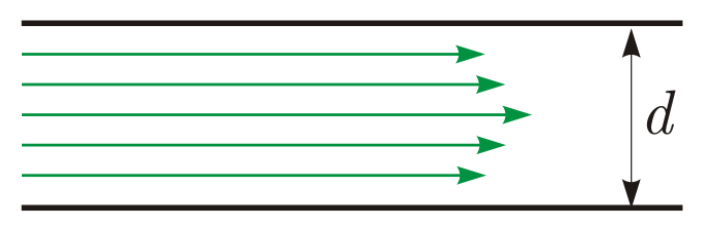
\includegraphics[width=\textwidth]{images/laminare-stroemung.png}
    \captionof{figure}{laminares Str\"omungsprofil \emph{Quelle:} Versuchsanleitung}
    \label{fig:laminaresProfil}
\end{minipage}
\begin{minipage}[t]{0.475\textwidth}
    \centering
    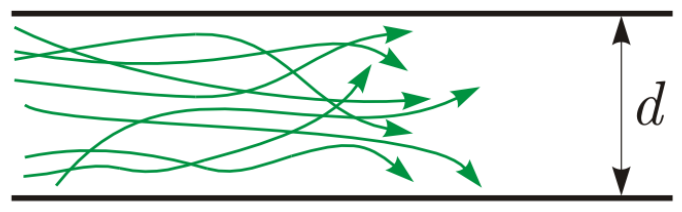
\includegraphics[width=\textwidth]{images/turbulente-stroemung.png}
    \captionof{figure}{turbulentes  Str\"omungsprofil \emph{Quelle:} Versuchsanleitung}
    \label{fig:turbulentesProfil}
\end{minipage}

\vspace{1em}
Zur Beurteilung, ob man es mit laminarem oder turbulentem Fluss zu tun hat, wird
die \emph{Reynoldszahl} herangezogen, die wie folgt definiert ist:

\begin{equation}
    \label{eq:reynolds}
    \mathit{Re} = \frac{\rho \cdot v_{\mathrm{m}} \cdot L}{\eta}
\end{equation}


\begin{conditions}
    \rho            & Dichte des Fluids \\
    v_{\mathrm{m}}  & mittlere Str\"omungsgeschwindigkeit \\
    L               & eine typische Abmessung \\
    \eta            & dynamische Viskosit\"at des Fluids (Materialkonstante) \\
\end{conditions}

Die Reynoldszahl  ist eine dimensionslose \"Ahnlichkeitszahl,  die dazu dient,
Systeme gleicher  Form aber verschiedener Abmessungen  miteinander vergleichen
zu k\"onnen. Die  Ursache ihrer  Notwendigkeit ergibt  sich daraus,  dass sich
Fluide auf verschiedenen Gr\"ossenskalen  nicht gleich verhalten. Zum Beispiel
ist Wasser f\"ur mikroskopische Lebewesen sehr z\"ahfl\"ussig, im Gegensatz zu
einem  Lebewesen  unserer  Gr\"ossenordnung. Selbst Luft  ist  f\"ur  kleinste
Lebewesen dickfl\"ussig.

Will  man das  Verhalten  eines modellierten  Systems (z.B. Flugzeugmodell  in
einem Windkanal) in  einem Fluid mit der Realit\"at  vergleichen, m\"ussen die
Reynoldszahlen des Modellversuchs und der Realit\"at \"ubereinstimmen.

Im Falle von zylindrischen Rohrleitungen  hat man experimentell bestimmt, dass
die  zu  verwendete  characteristische  L\"ange $L$  mit  dem  Rohrdurchmesser
gleichzusetzen  ist   und  dass  die   Str\"omung  bis  zu   einer  kritischen
Reynoldszahl $\mathit{Re}_{krit} \approx 2000$ noch laminar ist.

Es sei darauf hingewiesen, dass  die kritische Reynoldszahl von der Systemform
abh\"angt; f\"ur eine Trompete wird $\mathit{Re}_{krit}$ anders sein.


% ---------------------------------------------------------------------------- %
\subsubsection{Str\"omungsprofile}
\label{subsubsec:stromungsprofile}
% ---------------------------------------------------------------------------- %

Aufgrund der Reibung innerhalb eines Fluids ist die Str\"omungsgeschwindigkeit
innerhalb eines  Fluids meist \"ortlich variabel. Normalerweise  wird dies mit
einem Str\"omungsfeld  $\vec{v}(x,y,z)(t)$ beschrieben. Im  station\"aren Fall
f\"allt die Zeitabh\"angigkeit heraus und man erh\"alt $\vec{v}(x,y,z)$.

In  diesem  Versuch  werden lediglich  rotationssymmetrische  Str\"omungen  in
zylindrischen  Rohrleitungen   betrachtet,  womit  sich   das  Str\"omungsfeld
aufgrund radialer Symmetrie zu $\vec{v}(x,y,z) = \vec{v}(r)$ vereinfacht.

Liegt laminare Str\"omung vor, kann das Str\"omungsprofil analytisch berechnet
werden; das  Resultat ist das  Gesetz von Hagen-Poiseuille;  ein parabolisches
Str\"omungsprofil, abgebildet in Abbildung \ref{fig:hagenPoiseuille}.

\begin{equation}
    \label{eq:laminarprofile}
    v(r) = \frac{\Delta\,p \cdot R^2}{4 \cdot \eta \cdot l} \cdot \left( 1 - \frac{r^2}{R^2} \right) = v_{\mathrm{max}} \cdot \left( 1 - \frac{r^2}{R^2} \right)
\end{equation}


\begin{conditions}
    r                & radiale Position                                    \\
    R                & Radius der Rohrleitung                              \\
    \Delta\,p        & Druckdifferenz \"uber Leitungsst\"uck der L\"ange l \\
    \eta             & dynamische Viskosit\"at                             \\
    l                & L\"ange des betrachteten Rohrst\"uckes              \\
    v_{\mathrm{max}} & maximale Str\"omungsgeschwindigkeit                 \\
\end{conditions}

\begin{figure}[h!t]
    \centering
    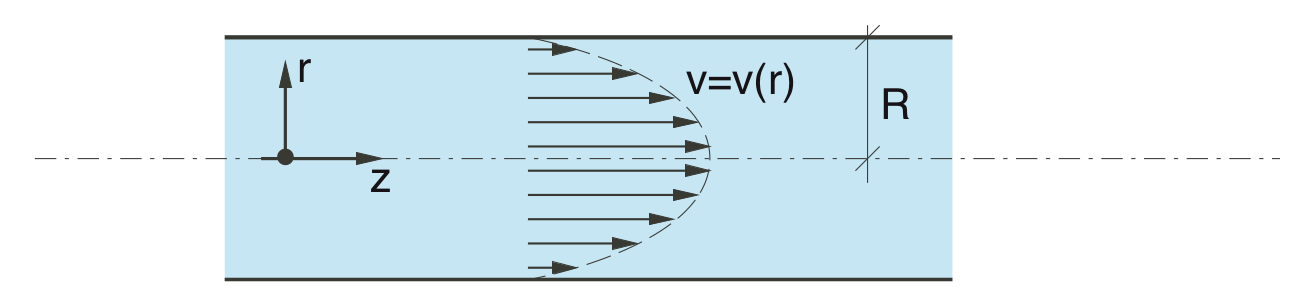
\includegraphics[width=0.67\textwidth]{images/hagen-poiseuille.png}
    \caption{Gesetz von Hagen-Poiseuille \emph{Quelle:} Versuchsanleitung}
    \label{fig:hagenPoiseuille}
\end{figure}

Will man den Volumenstrom bestimmen, ist dazu das Str\"omungsprofil \"uber den
Querschnitt zu  integrieren (aufgrund der radialen  Symmetrie vereinfacht sich
das Integral zu einer Integration \"uber den Radius):

\begin{equation}
    \label{eq:volumenstrom:laminar}
    \dot{V} = \int_{Rohrquerschnitt} v(r) \, \mathrm{d}F = \int_0^R v(r) \cdot 2 \pi r \cdot \mathrm{d}r
            = \frac{\pi \cdot R^2 \cdot v_{\mathrm{max}}}{2}
\end{equation}

Daraus    l\"asst    sich    nun     leicht    der    Zusammenhang    zwischen
durchschnittlicher   Str\"omungsgeschwindigkeit   $v_{\mathrm{m}}$   und   der
maximalen  Str\"omungsgeschwindigkeit  im  laminaren  Fall  $v_{\mathrm{max}}$
herleiten:

\begin{equation}
    \label{eq:vm_vmax:laminar}
    \frac{v_{\mathrm{m}}}{v_{\mathrm{max}}} = \frac{1}{2}
\end{equation}


Damit    sich    das     parabolische    Str\"omungsprofil    aus    Gleichung
\ref{eq:laminarprofile} ausbilden kann, ist  eine gen\"ugend lange Messleitung
erforderlich. Die  Ausbildung des  Str\"omungsprofils \"uber  die L\"ange  des
Rohres ist in Abbildung \ref{fig:ausbildungLaminareStromung} dargestellt.

\begin{figure}[h!t]
    \centering
    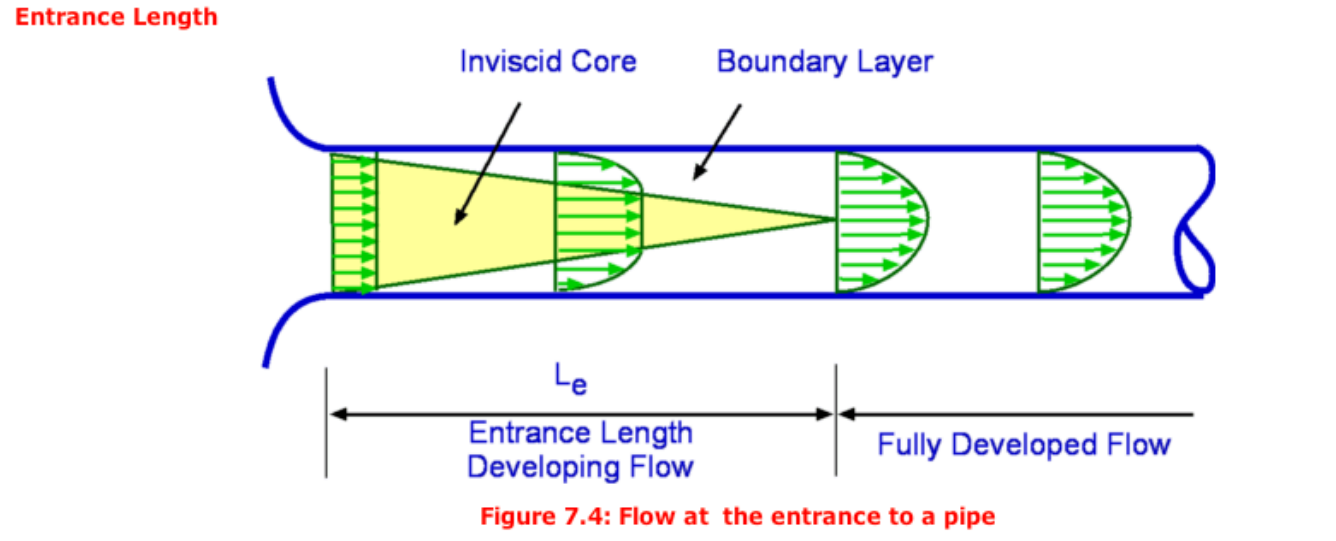
\includegraphics[width=0.67\textwidth]{images/ausbildung-laminares-stroemungsprofil.png}
    \caption{Ausbildung des laminaren Str\"omungsprofils \"ber die Rohrl\"ange}
    \label{fig:ausbildungLaminareStromung}
\end{figure}

Gem\"ass    Versuchsanleitung   w\"are    f\"ur   ein    perfektes   laminares
Str\"omungsprofil   eine  Messleitung   der  L\"ange   von  ca. \SI{5}{\meter}
erforderlich,  was  in  diesem  Versuch nicht  erreicht  wird. Die  Abweichung
des    Ver\"altnisses    $\frac{v_{\mathrm{max}}}{v_{\mathrm{m}}}$   vom    in
Gleichung  \ref{eq:vm_vmax:laminar} bestimmten  Ver\"altnis  ist in  Abbildung
\ref{fig:einlauf} dargestellt.

\begin{figure}[h!t]
    \centering
    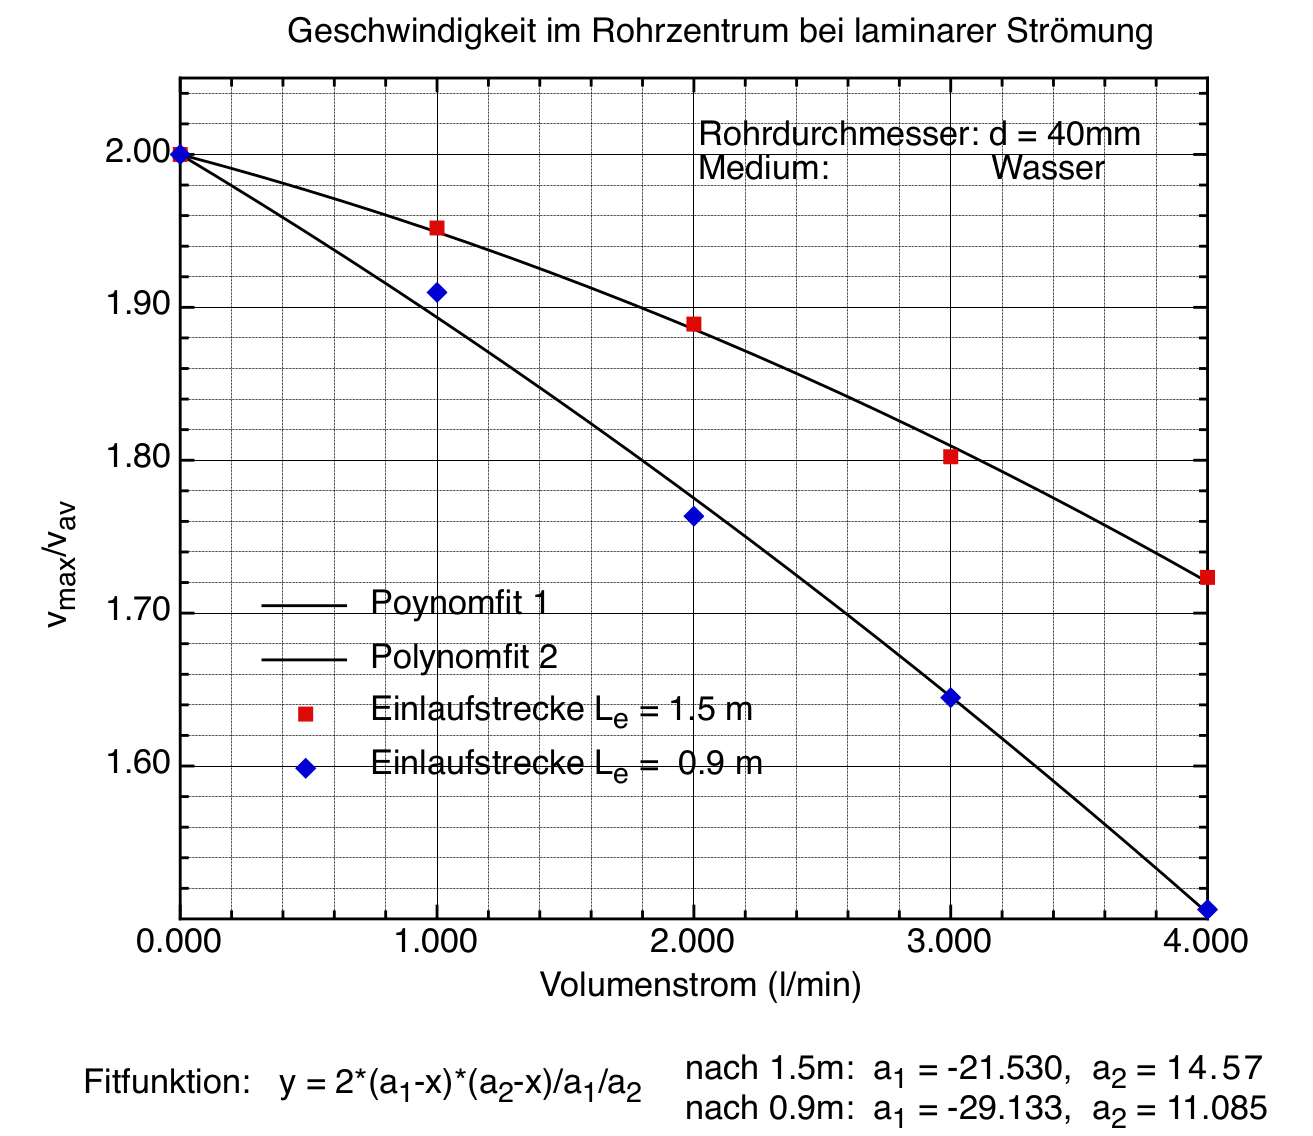
\includegraphics[width=0.67\textwidth]{images/einlauf.png}
    \caption{%
        Verh\"altnis  $\frac{v_{\mathrm{max}}}{v_{\mathrm{m}}}$   in  Funktion
        des     Volumenstroms      bei     zu      kurzen     Einlaufstrecken.
        \emph{Quelle:} Versuchsanleitung
    }
    \label{fig:einlauf}
\end{figure}
% TODO: length of tube


Man kann  auch den Zusammenhang  zwischen dem Volumenstrom und  dem Rohrradius
bei gleichem  Druckgef\"alle untersuchen. Dabei wird  f\"ur $v_{\mathrm{max}}$
der in Gleichung \ref{eq:laminarprofile}  bereits angetroffene Wert eingesetzt
und  die Formel  anschliessend  \"uber die  Fl\"ache integriert. Das  Resultat
lautet:

\begin{equation}
    \label{eq:q:r}
    \begin{split}
        \dot{V} &= \int_{0}^R \frac{\Delta\,p \cdot R^2}{4 \cdot \eta \cdot l} \cdot \left( 1 - \frac{r^2}{R^2} \right) \, \mathrm{d}r \\
                &= \frac{\pi \cdot R^4 \cdot \Delta \, p}{8 \cdot \eta \cdot l}
    \end{split}
\end{equation}

Es ergibt sich also eine Abh\"angigkeit vom Rohrradius in vierter Potenz!

Zur L\"osung  der Integrale aus Gleichungen  \ref{eq:volumenstrom:laminar} und
\ref{eq:q:r}  wurde SymPy  benutzt;  das zugeh\"orige  Script  kann in  Anhang
\ref{app:python:Qlaminar}  auf  Seite  \pageref{app:python:Qlaminar}  gefunden
werden.

Im turbulenten  Fall ist die  Sache nicht mehr  ganz so einfach. In  der Mitte
wird  das  Geschwindigkeitsprofil  abgeflacht  und  entlang  der  Wand  bilden
sich  eine  Grenzschicht  mit grossen  Geschwindigkeitsunterschieden  aus. Die
Geschwindigkeit nimmt gegen die Mitte des Rohres nur noch wenig zu.

\begin{figure}[h!t]
    \centering
    \resizebox{0.8\textwidth}{!}{%% Creator: Matplotlib, PGF backend
%%
%% To include the figure in your LaTeX document, write
%%   \input{<filename>.pgf}
%%
%% Make sure the required packages are loaded in your preamble
%%   \usepackage{pgf}
%%
%% Figures using additional raster images can only be included by \input if
%% they are in the same directory as the main LaTeX file. For loading figures
%% from other directories you can use the `import` package
%%   \usepackage{import}
%% and then include the figures with
%%   \import{<path to file>}{<filename>.pgf}
%%
%% Matplotlib used the following preamble
%%   \usepackage{fontspec}
%%   \setmainfont{Bitstream Vera Serif}
%%   \setsansfont{Bitstream Vera Sans}
%%   \setmonofont{Bitstream Vera Sans Mono}
%%
\begingroup%
\makeatletter%
\begin{pgfpicture}%
\pgfpathrectangle{\pgfpointorigin}{\pgfqpoint{8.000000in}{4.000000in}}%
\pgfusepath{use as bounding box, clip}%
\begin{pgfscope}%
\pgfsetbuttcap%
\pgfsetmiterjoin%
\definecolor{currentfill}{rgb}{1.000000,1.000000,1.000000}%
\pgfsetfillcolor{currentfill}%
\pgfsetlinewidth{0.000000pt}%
\definecolor{currentstroke}{rgb}{1.000000,1.000000,1.000000}%
\pgfsetstrokecolor{currentstroke}%
\pgfsetdash{}{0pt}%
\pgfpathmoveto{\pgfqpoint{0.000000in}{0.000000in}}%
\pgfpathlineto{\pgfqpoint{8.000000in}{0.000000in}}%
\pgfpathlineto{\pgfqpoint{8.000000in}{4.000000in}}%
\pgfpathlineto{\pgfqpoint{0.000000in}{4.000000in}}%
\pgfpathclose%
\pgfusepath{fill}%
\end{pgfscope}%
\begin{pgfscope}%
\pgfsetbuttcap%
\pgfsetmiterjoin%
\definecolor{currentfill}{rgb}{1.000000,1.000000,1.000000}%
\pgfsetfillcolor{currentfill}%
\pgfsetlinewidth{0.000000pt}%
\definecolor{currentstroke}{rgb}{0.000000,0.000000,0.000000}%
\pgfsetstrokecolor{currentstroke}%
\pgfsetstrokeopacity{0.000000}%
\pgfsetdash{}{0pt}%
\pgfpathmoveto{\pgfqpoint{0.800000in}{0.600000in}}%
\pgfpathlineto{\pgfqpoint{7.200000in}{0.600000in}}%
\pgfpathlineto{\pgfqpoint{7.200000in}{3.600000in}}%
\pgfpathlineto{\pgfqpoint{0.800000in}{3.600000in}}%
\pgfpathclose%
\pgfusepath{fill}%
\end{pgfscope}%
\begin{pgfscope}%
\pgfpathrectangle{\pgfqpoint{0.800000in}{0.600000in}}{\pgfqpoint{6.400000in}{3.000000in}} %
\pgfusepath{clip}%
\pgfsetrectcap%
\pgfsetroundjoin%
\pgfsetlinewidth{1.003750pt}%
\definecolor{currentstroke}{rgb}{0.000000,0.000000,1.000000}%
\pgfsetstrokecolor{currentstroke}%
\pgfsetdash{}{0pt}%
\pgfpathmoveto{\pgfqpoint{0.800000in}{3.600000in}}%
\pgfpathlineto{\pgfqpoint{1.277340in}{3.566280in}}%
\pgfpathlineto{\pgfqpoint{1.723276in}{3.532555in}}%
\pgfpathlineto{\pgfqpoint{2.131528in}{3.499496in}}%
\pgfpathlineto{\pgfqpoint{2.514656in}{3.466270in}}%
\pgfpathlineto{\pgfqpoint{2.866380in}{3.433589in}}%
\pgfpathlineto{\pgfqpoint{3.192981in}{3.401074in}}%
\pgfpathlineto{\pgfqpoint{3.500740in}{3.368212in}}%
\pgfpathlineto{\pgfqpoint{3.783376in}{3.335822in}}%
\pgfpathlineto{\pgfqpoint{4.047169in}{3.303363in}}%
\pgfpathlineto{\pgfqpoint{4.292120in}{3.270973in}}%
\pgfpathlineto{\pgfqpoint{4.518228in}{3.238828in}}%
\pgfpathlineto{\pgfqpoint{4.725494in}{3.207144in}}%
\pgfpathlineto{\pgfqpoint{4.920199in}{3.175116in}}%
\pgfpathlineto{\pgfqpoint{5.096061in}{3.143978in}}%
\pgfpathlineto{\pgfqpoint{5.259361in}{3.112863in}}%
\pgfpathlineto{\pgfqpoint{5.410100in}{3.081932in}}%
\pgfpathlineto{\pgfqpoint{5.548278in}{3.051392in}}%
\pgfpathlineto{\pgfqpoint{5.680174in}{3.019943in}}%
\pgfpathlineto{\pgfqpoint{5.799509in}{2.989209in}}%
\pgfpathlineto{\pgfqpoint{5.906283in}{2.959544in}}%
\pgfpathlineto{\pgfqpoint{6.006775in}{2.929418in}}%
\pgfpathlineto{\pgfqpoint{6.100987in}{2.898881in}}%
\pgfpathlineto{\pgfqpoint{6.188918in}{2.868001in}}%
\pgfpathlineto{\pgfqpoint{6.270569in}{2.836876in}}%
\pgfpathlineto{\pgfqpoint{6.345938in}{2.805639in}}%
\pgfpathlineto{\pgfqpoint{6.415027in}{2.774469in}}%
\pgfpathlineto{\pgfqpoint{6.477835in}{2.743600in}}%
\pgfpathlineto{\pgfqpoint{6.534362in}{2.713337in}}%
\pgfpathlineto{\pgfqpoint{6.584608in}{2.684064in}}%
\pgfpathlineto{\pgfqpoint{6.634854in}{2.652094in}}%
\pgfpathlineto{\pgfqpoint{6.678820in}{2.621439in}}%
\pgfpathlineto{\pgfqpoint{6.716505in}{2.592742in}}%
\pgfpathlineto{\pgfqpoint{6.754189in}{2.561329in}}%
\pgfpathlineto{\pgfqpoint{6.785593in}{2.532630in}}%
\pgfpathlineto{\pgfqpoint{6.816997in}{2.501120in}}%
\pgfpathlineto{\pgfqpoint{6.848401in}{2.466125in}}%
\pgfpathlineto{\pgfqpoint{6.873525in}{2.434988in}}%
\pgfpathlineto{\pgfqpoint{6.898648in}{2.400316in}}%
\pgfpathlineto{\pgfqpoint{6.923771in}{2.361104in}}%
\pgfpathlineto{\pgfqpoint{6.942613in}{2.327827in}}%
\pgfpathlineto{\pgfqpoint{6.961456in}{2.290194in}}%
\pgfpathlineto{\pgfqpoint{6.980298in}{2.246740in}}%
\pgfpathlineto{\pgfqpoint{6.992860in}{2.213417in}}%
\pgfpathlineto{\pgfqpoint{7.005421in}{2.175369in}}%
\pgfpathlineto{\pgfqpoint{7.017983in}{2.130849in}}%
\pgfpathlineto{\pgfqpoint{7.030544in}{2.076863in}}%
\pgfpathlineto{\pgfqpoint{7.043106in}{2.007553in}}%
\pgfpathlineto{\pgfqpoint{7.049387in}{1.963391in}}%
\pgfpathlineto{\pgfqpoint{7.055667in}{1.908495in}}%
\pgfpathlineto{\pgfqpoint{7.061948in}{1.834856in}}%
\pgfpathlineto{\pgfqpoint{7.068229in}{1.718438in}}%
\pgfpathlineto{\pgfqpoint{7.074510in}{0.600000in}}%
\pgfpathlineto{\pgfqpoint{7.074510in}{0.600000in}}%
\pgfusepath{stroke}%
\end{pgfscope}%
\begin{pgfscope}%
\pgfsetrectcap%
\pgfsetmiterjoin%
\pgfsetlinewidth{1.003750pt}%
\definecolor{currentstroke}{rgb}{0.000000,0.000000,0.000000}%
\pgfsetstrokecolor{currentstroke}%
\pgfsetdash{}{0pt}%
\pgfpathmoveto{\pgfqpoint{7.200000in}{0.600000in}}%
\pgfpathlineto{\pgfqpoint{7.200000in}{3.600000in}}%
\pgfusepath{stroke}%
\end{pgfscope}%
\begin{pgfscope}%
\pgfsetrectcap%
\pgfsetmiterjoin%
\pgfsetlinewidth{1.003750pt}%
\definecolor{currentstroke}{rgb}{0.000000,0.000000,0.000000}%
\pgfsetstrokecolor{currentstroke}%
\pgfsetdash{}{0pt}%
\pgfpathmoveto{\pgfqpoint{0.800000in}{0.600000in}}%
\pgfpathlineto{\pgfqpoint{0.800000in}{3.600000in}}%
\pgfusepath{stroke}%
\end{pgfscope}%
\begin{pgfscope}%
\pgfsetrectcap%
\pgfsetmiterjoin%
\pgfsetlinewidth{1.003750pt}%
\definecolor{currentstroke}{rgb}{0.000000,0.000000,0.000000}%
\pgfsetstrokecolor{currentstroke}%
\pgfsetdash{}{0pt}%
\pgfpathmoveto{\pgfqpoint{0.800000in}{0.600000in}}%
\pgfpathlineto{\pgfqpoint{7.200000in}{0.600000in}}%
\pgfusepath{stroke}%
\end{pgfscope}%
\begin{pgfscope}%
\pgfsetrectcap%
\pgfsetmiterjoin%
\pgfsetlinewidth{1.003750pt}%
\definecolor{currentstroke}{rgb}{0.000000,0.000000,0.000000}%
\pgfsetstrokecolor{currentstroke}%
\pgfsetdash{}{0pt}%
\pgfpathmoveto{\pgfqpoint{0.800000in}{3.600000in}}%
\pgfpathlineto{\pgfqpoint{7.200000in}{3.600000in}}%
\pgfusepath{stroke}%
\end{pgfscope}%
\begin{pgfscope}%
\pgfsetbuttcap%
\pgfsetroundjoin%
\definecolor{currentfill}{rgb}{0.000000,0.000000,0.000000}%
\pgfsetfillcolor{currentfill}%
\pgfsetlinewidth{0.501875pt}%
\definecolor{currentstroke}{rgb}{0.000000,0.000000,0.000000}%
\pgfsetstrokecolor{currentstroke}%
\pgfsetdash{}{0pt}%
\pgfsys@defobject{currentmarker}{\pgfqpoint{0.000000in}{0.000000in}}{\pgfqpoint{0.000000in}{0.055556in}}{%
\pgfpathmoveto{\pgfqpoint{0.000000in}{0.000000in}}%
\pgfpathlineto{\pgfqpoint{0.000000in}{0.055556in}}%
\pgfusepath{stroke,fill}%
}%
\begin{pgfscope}%
\pgfsys@transformshift{0.800000in}{0.600000in}%
\pgfsys@useobject{currentmarker}{}%
\end{pgfscope}%
\end{pgfscope}%
\begin{pgfscope}%
\pgfsetbuttcap%
\pgfsetroundjoin%
\definecolor{currentfill}{rgb}{0.000000,0.000000,0.000000}%
\pgfsetfillcolor{currentfill}%
\pgfsetlinewidth{0.501875pt}%
\definecolor{currentstroke}{rgb}{0.000000,0.000000,0.000000}%
\pgfsetstrokecolor{currentstroke}%
\pgfsetdash{}{0pt}%
\pgfsys@defobject{currentmarker}{\pgfqpoint{0.000000in}{-0.055556in}}{\pgfqpoint{0.000000in}{0.000000in}}{%
\pgfpathmoveto{\pgfqpoint{0.000000in}{0.000000in}}%
\pgfpathlineto{\pgfqpoint{0.000000in}{-0.055556in}}%
\pgfusepath{stroke,fill}%
}%
\begin{pgfscope}%
\pgfsys@transformshift{0.800000in}{3.600000in}%
\pgfsys@useobject{currentmarker}{}%
\end{pgfscope}%
\end{pgfscope}%
\begin{pgfscope}%
\pgftext[x=0.800000in,y=0.544444in,,top]{\rmfamily\fontsize{12.000000}{14.400000}\selectfont \(\displaystyle 0.0\)}%
\end{pgfscope}%
\begin{pgfscope}%
\pgfsetbuttcap%
\pgfsetroundjoin%
\definecolor{currentfill}{rgb}{0.000000,0.000000,0.000000}%
\pgfsetfillcolor{currentfill}%
\pgfsetlinewidth{0.501875pt}%
\definecolor{currentstroke}{rgb}{0.000000,0.000000,0.000000}%
\pgfsetstrokecolor{currentstroke}%
\pgfsetdash{}{0pt}%
\pgfsys@defobject{currentmarker}{\pgfqpoint{0.000000in}{0.000000in}}{\pgfqpoint{0.000000in}{0.055556in}}{%
\pgfpathmoveto{\pgfqpoint{0.000000in}{0.000000in}}%
\pgfpathlineto{\pgfqpoint{0.000000in}{0.055556in}}%
\pgfusepath{stroke,fill}%
}%
\begin{pgfscope}%
\pgfsys@transformshift{2.054902in}{0.600000in}%
\pgfsys@useobject{currentmarker}{}%
\end{pgfscope}%
\end{pgfscope}%
\begin{pgfscope}%
\pgfsetbuttcap%
\pgfsetroundjoin%
\definecolor{currentfill}{rgb}{0.000000,0.000000,0.000000}%
\pgfsetfillcolor{currentfill}%
\pgfsetlinewidth{0.501875pt}%
\definecolor{currentstroke}{rgb}{0.000000,0.000000,0.000000}%
\pgfsetstrokecolor{currentstroke}%
\pgfsetdash{}{0pt}%
\pgfsys@defobject{currentmarker}{\pgfqpoint{0.000000in}{-0.055556in}}{\pgfqpoint{0.000000in}{0.000000in}}{%
\pgfpathmoveto{\pgfqpoint{0.000000in}{0.000000in}}%
\pgfpathlineto{\pgfqpoint{0.000000in}{-0.055556in}}%
\pgfusepath{stroke,fill}%
}%
\begin{pgfscope}%
\pgfsys@transformshift{2.054902in}{3.600000in}%
\pgfsys@useobject{currentmarker}{}%
\end{pgfscope}%
\end{pgfscope}%
\begin{pgfscope}%
\pgftext[x=2.054902in,y=0.544444in,,top]{\rmfamily\fontsize{12.000000}{14.400000}\selectfont \(\displaystyle 0.2\)}%
\end{pgfscope}%
\begin{pgfscope}%
\pgfsetbuttcap%
\pgfsetroundjoin%
\definecolor{currentfill}{rgb}{0.000000,0.000000,0.000000}%
\pgfsetfillcolor{currentfill}%
\pgfsetlinewidth{0.501875pt}%
\definecolor{currentstroke}{rgb}{0.000000,0.000000,0.000000}%
\pgfsetstrokecolor{currentstroke}%
\pgfsetdash{}{0pt}%
\pgfsys@defobject{currentmarker}{\pgfqpoint{0.000000in}{0.000000in}}{\pgfqpoint{0.000000in}{0.055556in}}{%
\pgfpathmoveto{\pgfqpoint{0.000000in}{0.000000in}}%
\pgfpathlineto{\pgfqpoint{0.000000in}{0.055556in}}%
\pgfusepath{stroke,fill}%
}%
\begin{pgfscope}%
\pgfsys@transformshift{3.309804in}{0.600000in}%
\pgfsys@useobject{currentmarker}{}%
\end{pgfscope}%
\end{pgfscope}%
\begin{pgfscope}%
\pgfsetbuttcap%
\pgfsetroundjoin%
\definecolor{currentfill}{rgb}{0.000000,0.000000,0.000000}%
\pgfsetfillcolor{currentfill}%
\pgfsetlinewidth{0.501875pt}%
\definecolor{currentstroke}{rgb}{0.000000,0.000000,0.000000}%
\pgfsetstrokecolor{currentstroke}%
\pgfsetdash{}{0pt}%
\pgfsys@defobject{currentmarker}{\pgfqpoint{0.000000in}{-0.055556in}}{\pgfqpoint{0.000000in}{0.000000in}}{%
\pgfpathmoveto{\pgfqpoint{0.000000in}{0.000000in}}%
\pgfpathlineto{\pgfqpoint{0.000000in}{-0.055556in}}%
\pgfusepath{stroke,fill}%
}%
\begin{pgfscope}%
\pgfsys@transformshift{3.309804in}{3.600000in}%
\pgfsys@useobject{currentmarker}{}%
\end{pgfscope}%
\end{pgfscope}%
\begin{pgfscope}%
\pgftext[x=3.309804in,y=0.544444in,,top]{\rmfamily\fontsize{12.000000}{14.400000}\selectfont \(\displaystyle 0.4\)}%
\end{pgfscope}%
\begin{pgfscope}%
\pgfsetbuttcap%
\pgfsetroundjoin%
\definecolor{currentfill}{rgb}{0.000000,0.000000,0.000000}%
\pgfsetfillcolor{currentfill}%
\pgfsetlinewidth{0.501875pt}%
\definecolor{currentstroke}{rgb}{0.000000,0.000000,0.000000}%
\pgfsetstrokecolor{currentstroke}%
\pgfsetdash{}{0pt}%
\pgfsys@defobject{currentmarker}{\pgfqpoint{0.000000in}{0.000000in}}{\pgfqpoint{0.000000in}{0.055556in}}{%
\pgfpathmoveto{\pgfqpoint{0.000000in}{0.000000in}}%
\pgfpathlineto{\pgfqpoint{0.000000in}{0.055556in}}%
\pgfusepath{stroke,fill}%
}%
\begin{pgfscope}%
\pgfsys@transformshift{4.564706in}{0.600000in}%
\pgfsys@useobject{currentmarker}{}%
\end{pgfscope}%
\end{pgfscope}%
\begin{pgfscope}%
\pgfsetbuttcap%
\pgfsetroundjoin%
\definecolor{currentfill}{rgb}{0.000000,0.000000,0.000000}%
\pgfsetfillcolor{currentfill}%
\pgfsetlinewidth{0.501875pt}%
\definecolor{currentstroke}{rgb}{0.000000,0.000000,0.000000}%
\pgfsetstrokecolor{currentstroke}%
\pgfsetdash{}{0pt}%
\pgfsys@defobject{currentmarker}{\pgfqpoint{0.000000in}{-0.055556in}}{\pgfqpoint{0.000000in}{0.000000in}}{%
\pgfpathmoveto{\pgfqpoint{0.000000in}{0.000000in}}%
\pgfpathlineto{\pgfqpoint{0.000000in}{-0.055556in}}%
\pgfusepath{stroke,fill}%
}%
\begin{pgfscope}%
\pgfsys@transformshift{4.564706in}{3.600000in}%
\pgfsys@useobject{currentmarker}{}%
\end{pgfscope}%
\end{pgfscope}%
\begin{pgfscope}%
\pgftext[x=4.564706in,y=0.544444in,,top]{\rmfamily\fontsize{12.000000}{14.400000}\selectfont \(\displaystyle 0.6\)}%
\end{pgfscope}%
\begin{pgfscope}%
\pgfsetbuttcap%
\pgfsetroundjoin%
\definecolor{currentfill}{rgb}{0.000000,0.000000,0.000000}%
\pgfsetfillcolor{currentfill}%
\pgfsetlinewidth{0.501875pt}%
\definecolor{currentstroke}{rgb}{0.000000,0.000000,0.000000}%
\pgfsetstrokecolor{currentstroke}%
\pgfsetdash{}{0pt}%
\pgfsys@defobject{currentmarker}{\pgfqpoint{0.000000in}{0.000000in}}{\pgfqpoint{0.000000in}{0.055556in}}{%
\pgfpathmoveto{\pgfqpoint{0.000000in}{0.000000in}}%
\pgfpathlineto{\pgfqpoint{0.000000in}{0.055556in}}%
\pgfusepath{stroke,fill}%
}%
\begin{pgfscope}%
\pgfsys@transformshift{5.819608in}{0.600000in}%
\pgfsys@useobject{currentmarker}{}%
\end{pgfscope}%
\end{pgfscope}%
\begin{pgfscope}%
\pgfsetbuttcap%
\pgfsetroundjoin%
\definecolor{currentfill}{rgb}{0.000000,0.000000,0.000000}%
\pgfsetfillcolor{currentfill}%
\pgfsetlinewidth{0.501875pt}%
\definecolor{currentstroke}{rgb}{0.000000,0.000000,0.000000}%
\pgfsetstrokecolor{currentstroke}%
\pgfsetdash{}{0pt}%
\pgfsys@defobject{currentmarker}{\pgfqpoint{0.000000in}{-0.055556in}}{\pgfqpoint{0.000000in}{0.000000in}}{%
\pgfpathmoveto{\pgfqpoint{0.000000in}{0.000000in}}%
\pgfpathlineto{\pgfqpoint{0.000000in}{-0.055556in}}%
\pgfusepath{stroke,fill}%
}%
\begin{pgfscope}%
\pgfsys@transformshift{5.819608in}{3.600000in}%
\pgfsys@useobject{currentmarker}{}%
\end{pgfscope}%
\end{pgfscope}%
\begin{pgfscope}%
\pgftext[x=5.819608in,y=0.544444in,,top]{\rmfamily\fontsize{12.000000}{14.400000}\selectfont \(\displaystyle 0.8\)}%
\end{pgfscope}%
\begin{pgfscope}%
\pgfsetbuttcap%
\pgfsetroundjoin%
\definecolor{currentfill}{rgb}{0.000000,0.000000,0.000000}%
\pgfsetfillcolor{currentfill}%
\pgfsetlinewidth{0.501875pt}%
\definecolor{currentstroke}{rgb}{0.000000,0.000000,0.000000}%
\pgfsetstrokecolor{currentstroke}%
\pgfsetdash{}{0pt}%
\pgfsys@defobject{currentmarker}{\pgfqpoint{0.000000in}{0.000000in}}{\pgfqpoint{0.000000in}{0.055556in}}{%
\pgfpathmoveto{\pgfqpoint{0.000000in}{0.000000in}}%
\pgfpathlineto{\pgfqpoint{0.000000in}{0.055556in}}%
\pgfusepath{stroke,fill}%
}%
\begin{pgfscope}%
\pgfsys@transformshift{7.074510in}{0.600000in}%
\pgfsys@useobject{currentmarker}{}%
\end{pgfscope}%
\end{pgfscope}%
\begin{pgfscope}%
\pgfsetbuttcap%
\pgfsetroundjoin%
\definecolor{currentfill}{rgb}{0.000000,0.000000,0.000000}%
\pgfsetfillcolor{currentfill}%
\pgfsetlinewidth{0.501875pt}%
\definecolor{currentstroke}{rgb}{0.000000,0.000000,0.000000}%
\pgfsetstrokecolor{currentstroke}%
\pgfsetdash{}{0pt}%
\pgfsys@defobject{currentmarker}{\pgfqpoint{0.000000in}{-0.055556in}}{\pgfqpoint{0.000000in}{0.000000in}}{%
\pgfpathmoveto{\pgfqpoint{0.000000in}{0.000000in}}%
\pgfpathlineto{\pgfqpoint{0.000000in}{-0.055556in}}%
\pgfusepath{stroke,fill}%
}%
\begin{pgfscope}%
\pgfsys@transformshift{7.074510in}{3.600000in}%
\pgfsys@useobject{currentmarker}{}%
\end{pgfscope}%
\end{pgfscope}%
\begin{pgfscope}%
\pgftext[x=7.074510in,y=0.544444in,,top]{\rmfamily\fontsize{12.000000}{14.400000}\selectfont \(\displaystyle 1.0\)}%
\end{pgfscope}%
\begin{pgfscope}%
\pgftext[x=4.000000in,y=0.313705in,,top]{\rmfamily\fontsize{12.000000}{14.400000}\selectfont Radius, normiert (b. E.)}%
\end{pgfscope}%
\begin{pgfscope}%
\pgfsetbuttcap%
\pgfsetroundjoin%
\definecolor{currentfill}{rgb}{0.000000,0.000000,0.000000}%
\pgfsetfillcolor{currentfill}%
\pgfsetlinewidth{0.501875pt}%
\definecolor{currentstroke}{rgb}{0.000000,0.000000,0.000000}%
\pgfsetstrokecolor{currentstroke}%
\pgfsetdash{}{0pt}%
\pgfsys@defobject{currentmarker}{\pgfqpoint{0.000000in}{0.000000in}}{\pgfqpoint{0.055556in}{0.000000in}}{%
\pgfpathmoveto{\pgfqpoint{0.000000in}{0.000000in}}%
\pgfpathlineto{\pgfqpoint{0.055556in}{0.000000in}}%
\pgfusepath{stroke,fill}%
}%
\begin{pgfscope}%
\pgfsys@transformshift{0.800000in}{0.600000in}%
\pgfsys@useobject{currentmarker}{}%
\end{pgfscope}%
\end{pgfscope}%
\begin{pgfscope}%
\pgfsetbuttcap%
\pgfsetroundjoin%
\definecolor{currentfill}{rgb}{0.000000,0.000000,0.000000}%
\pgfsetfillcolor{currentfill}%
\pgfsetlinewidth{0.501875pt}%
\definecolor{currentstroke}{rgb}{0.000000,0.000000,0.000000}%
\pgfsetstrokecolor{currentstroke}%
\pgfsetdash{}{0pt}%
\pgfsys@defobject{currentmarker}{\pgfqpoint{-0.055556in}{0.000000in}}{\pgfqpoint{0.000000in}{0.000000in}}{%
\pgfpathmoveto{\pgfqpoint{0.000000in}{0.000000in}}%
\pgfpathlineto{\pgfqpoint{-0.055556in}{0.000000in}}%
\pgfusepath{stroke,fill}%
}%
\begin{pgfscope}%
\pgfsys@transformshift{7.200000in}{0.600000in}%
\pgfsys@useobject{currentmarker}{}%
\end{pgfscope}%
\end{pgfscope}%
\begin{pgfscope}%
\pgftext[x=0.744444in,y=0.600000in,right,]{\rmfamily\fontsize{12.000000}{14.400000}\selectfont \(\displaystyle 0.0\)}%
\end{pgfscope}%
\begin{pgfscope}%
\pgfsetbuttcap%
\pgfsetroundjoin%
\definecolor{currentfill}{rgb}{0.000000,0.000000,0.000000}%
\pgfsetfillcolor{currentfill}%
\pgfsetlinewidth{0.501875pt}%
\definecolor{currentstroke}{rgb}{0.000000,0.000000,0.000000}%
\pgfsetstrokecolor{currentstroke}%
\pgfsetdash{}{0pt}%
\pgfsys@defobject{currentmarker}{\pgfqpoint{0.000000in}{0.000000in}}{\pgfqpoint{0.055556in}{0.000000in}}{%
\pgfpathmoveto{\pgfqpoint{0.000000in}{0.000000in}}%
\pgfpathlineto{\pgfqpoint{0.055556in}{0.000000in}}%
\pgfusepath{stroke,fill}%
}%
\begin{pgfscope}%
\pgfsys@transformshift{0.800000in}{1.200000in}%
\pgfsys@useobject{currentmarker}{}%
\end{pgfscope}%
\end{pgfscope}%
\begin{pgfscope}%
\pgfsetbuttcap%
\pgfsetroundjoin%
\definecolor{currentfill}{rgb}{0.000000,0.000000,0.000000}%
\pgfsetfillcolor{currentfill}%
\pgfsetlinewidth{0.501875pt}%
\definecolor{currentstroke}{rgb}{0.000000,0.000000,0.000000}%
\pgfsetstrokecolor{currentstroke}%
\pgfsetdash{}{0pt}%
\pgfsys@defobject{currentmarker}{\pgfqpoint{-0.055556in}{0.000000in}}{\pgfqpoint{0.000000in}{0.000000in}}{%
\pgfpathmoveto{\pgfqpoint{0.000000in}{0.000000in}}%
\pgfpathlineto{\pgfqpoint{-0.055556in}{0.000000in}}%
\pgfusepath{stroke,fill}%
}%
\begin{pgfscope}%
\pgfsys@transformshift{7.200000in}{1.200000in}%
\pgfsys@useobject{currentmarker}{}%
\end{pgfscope}%
\end{pgfscope}%
\begin{pgfscope}%
\pgftext[x=0.744444in,y=1.200000in,right,]{\rmfamily\fontsize{12.000000}{14.400000}\selectfont \(\displaystyle 0.2\)}%
\end{pgfscope}%
\begin{pgfscope}%
\pgfsetbuttcap%
\pgfsetroundjoin%
\definecolor{currentfill}{rgb}{0.000000,0.000000,0.000000}%
\pgfsetfillcolor{currentfill}%
\pgfsetlinewidth{0.501875pt}%
\definecolor{currentstroke}{rgb}{0.000000,0.000000,0.000000}%
\pgfsetstrokecolor{currentstroke}%
\pgfsetdash{}{0pt}%
\pgfsys@defobject{currentmarker}{\pgfqpoint{0.000000in}{0.000000in}}{\pgfqpoint{0.055556in}{0.000000in}}{%
\pgfpathmoveto{\pgfqpoint{0.000000in}{0.000000in}}%
\pgfpathlineto{\pgfqpoint{0.055556in}{0.000000in}}%
\pgfusepath{stroke,fill}%
}%
\begin{pgfscope}%
\pgfsys@transformshift{0.800000in}{1.800000in}%
\pgfsys@useobject{currentmarker}{}%
\end{pgfscope}%
\end{pgfscope}%
\begin{pgfscope}%
\pgfsetbuttcap%
\pgfsetroundjoin%
\definecolor{currentfill}{rgb}{0.000000,0.000000,0.000000}%
\pgfsetfillcolor{currentfill}%
\pgfsetlinewidth{0.501875pt}%
\definecolor{currentstroke}{rgb}{0.000000,0.000000,0.000000}%
\pgfsetstrokecolor{currentstroke}%
\pgfsetdash{}{0pt}%
\pgfsys@defobject{currentmarker}{\pgfqpoint{-0.055556in}{0.000000in}}{\pgfqpoint{0.000000in}{0.000000in}}{%
\pgfpathmoveto{\pgfqpoint{0.000000in}{0.000000in}}%
\pgfpathlineto{\pgfqpoint{-0.055556in}{0.000000in}}%
\pgfusepath{stroke,fill}%
}%
\begin{pgfscope}%
\pgfsys@transformshift{7.200000in}{1.800000in}%
\pgfsys@useobject{currentmarker}{}%
\end{pgfscope}%
\end{pgfscope}%
\begin{pgfscope}%
\pgftext[x=0.744444in,y=1.800000in,right,]{\rmfamily\fontsize{12.000000}{14.400000}\selectfont \(\displaystyle 0.4\)}%
\end{pgfscope}%
\begin{pgfscope}%
\pgfsetbuttcap%
\pgfsetroundjoin%
\definecolor{currentfill}{rgb}{0.000000,0.000000,0.000000}%
\pgfsetfillcolor{currentfill}%
\pgfsetlinewidth{0.501875pt}%
\definecolor{currentstroke}{rgb}{0.000000,0.000000,0.000000}%
\pgfsetstrokecolor{currentstroke}%
\pgfsetdash{}{0pt}%
\pgfsys@defobject{currentmarker}{\pgfqpoint{0.000000in}{0.000000in}}{\pgfqpoint{0.055556in}{0.000000in}}{%
\pgfpathmoveto{\pgfqpoint{0.000000in}{0.000000in}}%
\pgfpathlineto{\pgfqpoint{0.055556in}{0.000000in}}%
\pgfusepath{stroke,fill}%
}%
\begin{pgfscope}%
\pgfsys@transformshift{0.800000in}{2.400000in}%
\pgfsys@useobject{currentmarker}{}%
\end{pgfscope}%
\end{pgfscope}%
\begin{pgfscope}%
\pgfsetbuttcap%
\pgfsetroundjoin%
\definecolor{currentfill}{rgb}{0.000000,0.000000,0.000000}%
\pgfsetfillcolor{currentfill}%
\pgfsetlinewidth{0.501875pt}%
\definecolor{currentstroke}{rgb}{0.000000,0.000000,0.000000}%
\pgfsetstrokecolor{currentstroke}%
\pgfsetdash{}{0pt}%
\pgfsys@defobject{currentmarker}{\pgfqpoint{-0.055556in}{0.000000in}}{\pgfqpoint{0.000000in}{0.000000in}}{%
\pgfpathmoveto{\pgfqpoint{0.000000in}{0.000000in}}%
\pgfpathlineto{\pgfqpoint{-0.055556in}{0.000000in}}%
\pgfusepath{stroke,fill}%
}%
\begin{pgfscope}%
\pgfsys@transformshift{7.200000in}{2.400000in}%
\pgfsys@useobject{currentmarker}{}%
\end{pgfscope}%
\end{pgfscope}%
\begin{pgfscope}%
\pgftext[x=0.744444in,y=2.400000in,right,]{\rmfamily\fontsize{12.000000}{14.400000}\selectfont \(\displaystyle 0.6\)}%
\end{pgfscope}%
\begin{pgfscope}%
\pgfsetbuttcap%
\pgfsetroundjoin%
\definecolor{currentfill}{rgb}{0.000000,0.000000,0.000000}%
\pgfsetfillcolor{currentfill}%
\pgfsetlinewidth{0.501875pt}%
\definecolor{currentstroke}{rgb}{0.000000,0.000000,0.000000}%
\pgfsetstrokecolor{currentstroke}%
\pgfsetdash{}{0pt}%
\pgfsys@defobject{currentmarker}{\pgfqpoint{0.000000in}{0.000000in}}{\pgfqpoint{0.055556in}{0.000000in}}{%
\pgfpathmoveto{\pgfqpoint{0.000000in}{0.000000in}}%
\pgfpathlineto{\pgfqpoint{0.055556in}{0.000000in}}%
\pgfusepath{stroke,fill}%
}%
\begin{pgfscope}%
\pgfsys@transformshift{0.800000in}{3.000000in}%
\pgfsys@useobject{currentmarker}{}%
\end{pgfscope}%
\end{pgfscope}%
\begin{pgfscope}%
\pgfsetbuttcap%
\pgfsetroundjoin%
\definecolor{currentfill}{rgb}{0.000000,0.000000,0.000000}%
\pgfsetfillcolor{currentfill}%
\pgfsetlinewidth{0.501875pt}%
\definecolor{currentstroke}{rgb}{0.000000,0.000000,0.000000}%
\pgfsetstrokecolor{currentstroke}%
\pgfsetdash{}{0pt}%
\pgfsys@defobject{currentmarker}{\pgfqpoint{-0.055556in}{0.000000in}}{\pgfqpoint{0.000000in}{0.000000in}}{%
\pgfpathmoveto{\pgfqpoint{0.000000in}{0.000000in}}%
\pgfpathlineto{\pgfqpoint{-0.055556in}{0.000000in}}%
\pgfusepath{stroke,fill}%
}%
\begin{pgfscope}%
\pgfsys@transformshift{7.200000in}{3.000000in}%
\pgfsys@useobject{currentmarker}{}%
\end{pgfscope}%
\end{pgfscope}%
\begin{pgfscope}%
\pgftext[x=0.744444in,y=3.000000in,right,]{\rmfamily\fontsize{12.000000}{14.400000}\selectfont \(\displaystyle 0.8\)}%
\end{pgfscope}%
\begin{pgfscope}%
\pgfsetbuttcap%
\pgfsetroundjoin%
\definecolor{currentfill}{rgb}{0.000000,0.000000,0.000000}%
\pgfsetfillcolor{currentfill}%
\pgfsetlinewidth{0.501875pt}%
\definecolor{currentstroke}{rgb}{0.000000,0.000000,0.000000}%
\pgfsetstrokecolor{currentstroke}%
\pgfsetdash{}{0pt}%
\pgfsys@defobject{currentmarker}{\pgfqpoint{0.000000in}{0.000000in}}{\pgfqpoint{0.055556in}{0.000000in}}{%
\pgfpathmoveto{\pgfqpoint{0.000000in}{0.000000in}}%
\pgfpathlineto{\pgfqpoint{0.055556in}{0.000000in}}%
\pgfusepath{stroke,fill}%
}%
\begin{pgfscope}%
\pgfsys@transformshift{0.800000in}{3.600000in}%
\pgfsys@useobject{currentmarker}{}%
\end{pgfscope}%
\end{pgfscope}%
\begin{pgfscope}%
\pgfsetbuttcap%
\pgfsetroundjoin%
\definecolor{currentfill}{rgb}{0.000000,0.000000,0.000000}%
\pgfsetfillcolor{currentfill}%
\pgfsetlinewidth{0.501875pt}%
\definecolor{currentstroke}{rgb}{0.000000,0.000000,0.000000}%
\pgfsetstrokecolor{currentstroke}%
\pgfsetdash{}{0pt}%
\pgfsys@defobject{currentmarker}{\pgfqpoint{-0.055556in}{0.000000in}}{\pgfqpoint{0.000000in}{0.000000in}}{%
\pgfpathmoveto{\pgfqpoint{0.000000in}{0.000000in}}%
\pgfpathlineto{\pgfqpoint{-0.055556in}{0.000000in}}%
\pgfusepath{stroke,fill}%
}%
\begin{pgfscope}%
\pgfsys@transformshift{7.200000in}{3.600000in}%
\pgfsys@useobject{currentmarker}{}%
\end{pgfscope}%
\end{pgfscope}%
\begin{pgfscope}%
\pgftext[x=0.744444in,y=3.600000in,right,]{\rmfamily\fontsize{12.000000}{14.400000}\selectfont \(\displaystyle 1.0\)}%
\end{pgfscope}%
\begin{pgfscope}%
\pgftext[x=0.466476in,y=2.100000in,,bottom,rotate=90.000000]{\rmfamily\fontsize{12.000000}{14.400000}\selectfont Flussgeschwindigkeit, normiert (b. E.)}%
\end{pgfscope}%
\begin{pgfscope}%
\pgftext[x=4.000000in,y=3.669444in,,base]{\rmfamily\fontsize{14.400000}{17.280000}\selectfont Geschwindigkeitsprofil, turbulent}%
\end{pgfscope}%
\end{pgfpicture}%
\makeatother%
\endgroup%
}
    \caption{%
        Turbulentes   Str\"omungsprofil   (eine  Rohrh\"alfte),   vereinfachte
        Darstellung   basierend    auf   dem   Potenzgesetz    aus   Gleichung
        \ref{eq:potenzgesetz}.
    }
    \label{fig:turbProfile}
\end{figure}

H\"aufig kommt  in dieser Situation ein  ph\"anomenologisches Potenzgesetz zur
Anwending:

\begin{equation}
    \label{eq:potenzgesetz}
    v(r) = v_{\mathrm{max}} \cdot \left( 1 - \frac{r}{R} \right)^{\frac{1}{k}}
\end{equation}

\begin{conditions}
    v_{\mathrm{max}} & maximale Str\"omungsgeschwindigkeit \\
    r                & radiale Position                    \\
    R                & Radius Leitung                      \\
    k                & Modellierungsparameter; abh\"angig von Reynoldszahl, experimentell zu bestimmen \\
\end{conditions}
Typische Werte f\"ur $k$ sind:

\begin{conditions}
    k = 6 & $\mathit{Re} \approx 4000$ \\
    k = 7 & $\mathit{Re} \approx 10^5$ \\
    k = 9 & $\mathit{Re} \approx 10^6$ \\
\end{conditions}

Will  man  hier  den  Volumenstrom  bestimmen,  ist  ebenfalls  $v(r)$  \"uber
den  Querschnitt  zu  integrieren. Anschliessend   kann  daraus  die  mittlere
Str\"omungsgeschwindigkeit  und  das   Verh\"altnis  derselben  zur  maximalen
Str\"omungsgeschwindigkeit gebildet werden.

\begin{align}
    \label{eq:turbulent:Q}
    v(r) &= v_{max} \cdot \left( 1 - \frac{r}{R} \right) ^ \frac{1}{k}
    \\
    \dot{V} &= \int_0^R \! v(r) \cdot 2 \cdot \pi \cdot r \, \mathrm{d}r = \frac{2 \cdot \pi \cdot v_{\mathrm{max}} \cdot R^2 \cdot k^2}{(k + 1) \cdot (2k + 1)}
    \\
    v_{\mathrm{m}} &= \frac{\dot{V}}{R^2 \cdot \pi} = \frac{2 \cdot v_{\mathrm{max}} \cdot k^2}{(k + 1) \cdot (2k + 1)}
    \\
    \frac{v_{\mathrm{m}}}{v_{\mathrm{max}}} &= \frac{2 \cdot k^2}{(k + 1) \cdot (2k + 1)}
\end{align}

Auch  hier  wurde SymPy  eingesetzt. Das  zugeh\"orige  Script ist  in  Anhang
\ref{app:python:Qturb} auf Seite \pageref{app:python:Qturb} zu finden.

